\documentclass[11pt]{article}
\usepackage{../problem-collection}

\begin{document}
\selectlanguage{english}

\begin{titlepage}
	\centering
	\vspace{10cm}
	{\sffamily\Huge \mbox{200 ESTONIAN PHYSICS OLYMPIAD}\\ PROBLEMS FROM YEARS\\ 2012 -- 2018\par}
	\vspace{1cm}
	{\Large With hints and solutions\par}
	\vfill
	{\Large Compiled by Taavet Kalda\par}
	\vspace{1cm}
	{\Large Translated by Rael Kalda}

	\vfill

	% Bottom of the page
	{\large 2018}
\end{titlepage}

\addtocounter{page}{1}
\mbox{}\vfill

\textcopyright~Copyright: Estonian Mathematical Society, Tallinn University of Technology,
University of Tartu, authors of the problems and Taavet Kalda.
\vspace{0.5\baselineskip}

The compilation of the problem book was supported by: Estonian Mathematical Society's fund ``Benoit Mandelbroti Jälgedes'', Robert Kitt and Tallinn University of Technology.
\vspace{0.5\baselineskip}

Publisher Tallinn University of Technology's pre-study department
\newpage

\tableofcontents
\newpage

{\setlength{\parindent}{24pt}
\section{Introduction}

This book contains 200 high school physics problems from the regional rounds, national rounds, and the open competitions of the Estonian physics olympiads.

Each problem comes with a short hint for students who are stuck on problems but do not want to look at the solutions just yet. The topics have been sorted based on their topics and the level of difficulty. The difficulty is marked with up to five stars. To make the searching of problems easier, a prefix is attached before the problem numbers, \enquote{P} for problem statements, \enquote{H} for hints and \enquote{S} for solutions. For example, the statement of problem 133 is denoted with P133. Furthermore, the name of the author and the round are written next to the title of the problem alongside with a short abbreviation of the form P 1, G 1 etc, where the letters correspond to middle school and high school respectively. G 9 would for example stand for the ninth problem in the high school division.

During the assembly of the problem book, four problems were removed due to various reasons and they were replaced with problems from 2011's open physics competition.}
\newpage
\setlength{\parindent}{0pt}

        \section{Problems}
        \toggleStatement
        \subsection{\protect\StrSubstitute{Dynamics}{-}{ }}

\graphicspath{{../problems/}}

% P1
\setAuthor{Erkki Tempel}
\setRound{piirkonnavoor}
\setYear{2014}
\setNumber{G 1}
\setDifficulty{1}
\setTopic{Dünaamika}

\prob{Flying bottle}
\probeng
A hole with an area of $S$ has been made in the bottom of a half-liter bottle. The bottle has $m$ grams of water in it. The lid of the bottle is removed and the bottle is thrown in the air with a starting speed of $v$. How fast is the water flowing out of the hole when the bottle is still moving up? How fast is it flowing out when the bottle is falling down? Explain.
\probend
\bigskip

% P2
\setAuthor{Erkki Tempel}
\setRound{piirkonnavoor}
\setYear{2014}
\setNumber{G 2}
\setDifficulty{1}
\setTopic{Dünaamika}

\prob{Cheburashka and nuts}
\probeng
Cheburashka is sitting on the roof of the last wagon of the train and is throwing down nuts. He throws two nuts, one of them flying horizontally opposite to the motion of the train with an initial speed $u$, and the other one perpendicularly to the line of motion with the same initial speed $u$. The train is moving uniformly and rectilinearly with a velocity of $v$ and the nuts are thrown at a height of $h$ from the ground. How far from each other will the nuts land? Do not account for air resistance.
\probend
\bigskip

% P3
\setAuthor{Mihkel Rähn}
\setRound{lahtine}
\setYear{2016}
\setNumber{G 2}
\setDifficulty{1}
\setTopic{Dünaamika}

\prob{Curve}
\probeng
A car with a speed of $v=\SI{90}{km/h}$ is driving through a curve of radius $R=\SI{250}{m}$. How big must the road’s sideways slant be in degrees so that the people in the car wouldn’t feel any side force from the curve? The gravitational acceleration is $g=\SI{9.8}{m/s^{2}}$.
\probend
\bigskip

% P4
\setAuthor{Eero Vaher}
\setRound{lahtine}
\setYear{2012}
\setNumber{G 2}
\setDifficulty{2}
\setTopic{Dünaamika}

\prob{Lost wallet}
\probeng
A Ski jumping hill’s track is situated on a slope with an angle of $\alpha$. The track’s take-off platform is horizontal. The ski jumper began the in-run at a height of $h$ relative to the take-off platform, but right at the start, his wallet fell out of his pocket. How far from the take-off will the wallet land (along the horizontal axis) if the wallet is moving without friction?
\probend
\bigskip

% P5
\setAuthor{Taavi Pungas}
\setRound{lahtine}
\setYear{2013}
\setNumber{G 1}
\setDifficulty{2}
\setTopic{Dünaamika}

\prob{Rock}
\probeng
Juku found a hemispherical rock sticking up from the ground. Measuring its circumference with a tape he got a result of $a=\SI{2,4}{m}$. Next he took a match box and started to slowly move it down from top of the hemisphere, until the box finally slid off the rock. Measuring along the hemisphere with a tape, Juku found that the distance from the tip of the rock to the point where the box slid off was $b=\SI{20}{cm}$. What was the coefficient of friction between the rock and the match box?
\probend
\bigskip

% P6
\setAuthor{Taavi Pungas}
\setRound{piirkonnavoor}
\setYear{2013}
\setNumber{G 4}
\setDifficulty{2}
\setTopic{Dünaamika}

\prob{Sledge}
\probeng
The time it took a kid to sledge down from an evenly sloped hill of height $h=\SI{2,0}{m}$ was $t=\SI{3,0}{s}$. What was the minimal angle of inclination $\alpha$ of the hill if the kid started to sledge from rest?
\probend
\bigskip

% P7
\setAuthor{Taivo Pungas}
\setRound{lõppvoor}
\setYear{2013}
\setNumber{G 2}
\setDifficulty{2}
\setTopic{Dünaamika}

\prob{Ball}
\probeng
Madis studied an audio recording of a bouncing ball with a computer program and got a graph shown below which shows the shape of the audio signal. Find the maximal height of the ball after the first bounce if it is known that the ball rose exactly 1 m high after the third bounce.
\begin{center}
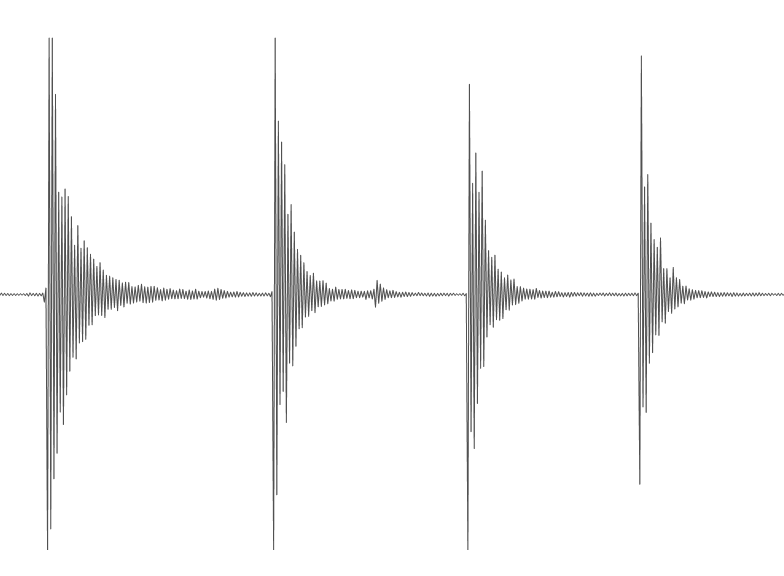
\includegraphics[width=0.5\textwidth]{2013-v3g-02-pall}%
\end{center}
\probend
\bigskip

% P8
\setAuthor{Mihkel Rähn}
\setRound{lahtine}
\setYear{2014}
\setNumber{G 1}
\setDifficulty{2}
\setTopic{Dünaamika}

\prob{Freight train}
\probeng
A freight train of mass $m=\SI{5000}{t}$ is carried by a locomotive of power $N=\SI{2500}{kW}$. Coefficient of rolling friction between the wheels and rails is $\mu=\SI{0,002}{}$.\\
a) Find the speed $v_1$ of the train on a horizontal road.\\
b) Find the speed $v_2$ of the train on a rise of one centimeter per meter.\\
Do not account for air resistance.
\probend
\bigskip

% P9
\setAuthor{Andreas Valdmann}
\setRound{lahtine}
\setYear{2014}
\setNumber{G 2}
\setDifficulty{2}
\setTopic{Dünaamika}

\prob{Vacuum cannon}
\probeng
Pictured below is a so-called vacuum cannon. To load it, a ball meant for ammunition is put into the left end of the vacuum cannon. Next, both ends of the tube are covered with an easily rupturing airproof membrane, for example foil, and then the air is pumped out of the tube. The vacuum cannon is now ready for firing. For firing, the membrane on the left is intentionally ruptured. As a result the ball starts to charge towards the right end of the tube. If the tube is long enough the ball ruptures the membrane on the right end and is fired out of the tube. Let us say that the diameter of the ball is equal to the inner diameter of the tube $d=\SI{4,0}{cm}$, the ball’s mass is $m=\SI{24}{g}$ and before the firing the ball is positioned at a distance $l=\SI{150}{cm}$ from the right end of the tube. What is the speed of the ball directly before rupturing the membrane on the right? Air pressure is $P_0=\SI{100}{kPa}$. Do not account for friction.
\begin{center}
  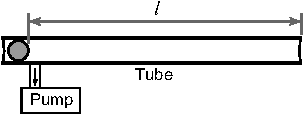
\includegraphics[width=0.75\textwidth]{2014-lahg-02-vaakumkahur_ing}
\end{center}
\probend
\bigskip

% P10
\setAuthor{EFO žürii}
\setRound{lahtine}
\setYear{2016}
\setNumber{G 1}
\setDifficulty{2}
\setTopic{Dünaamika}

\prob{Toy cannon}
\probeng
\begin{wrapfigure}[8]{r}{0.5\textwidth}
  \vspace{-20pt}
  \begin{center}
    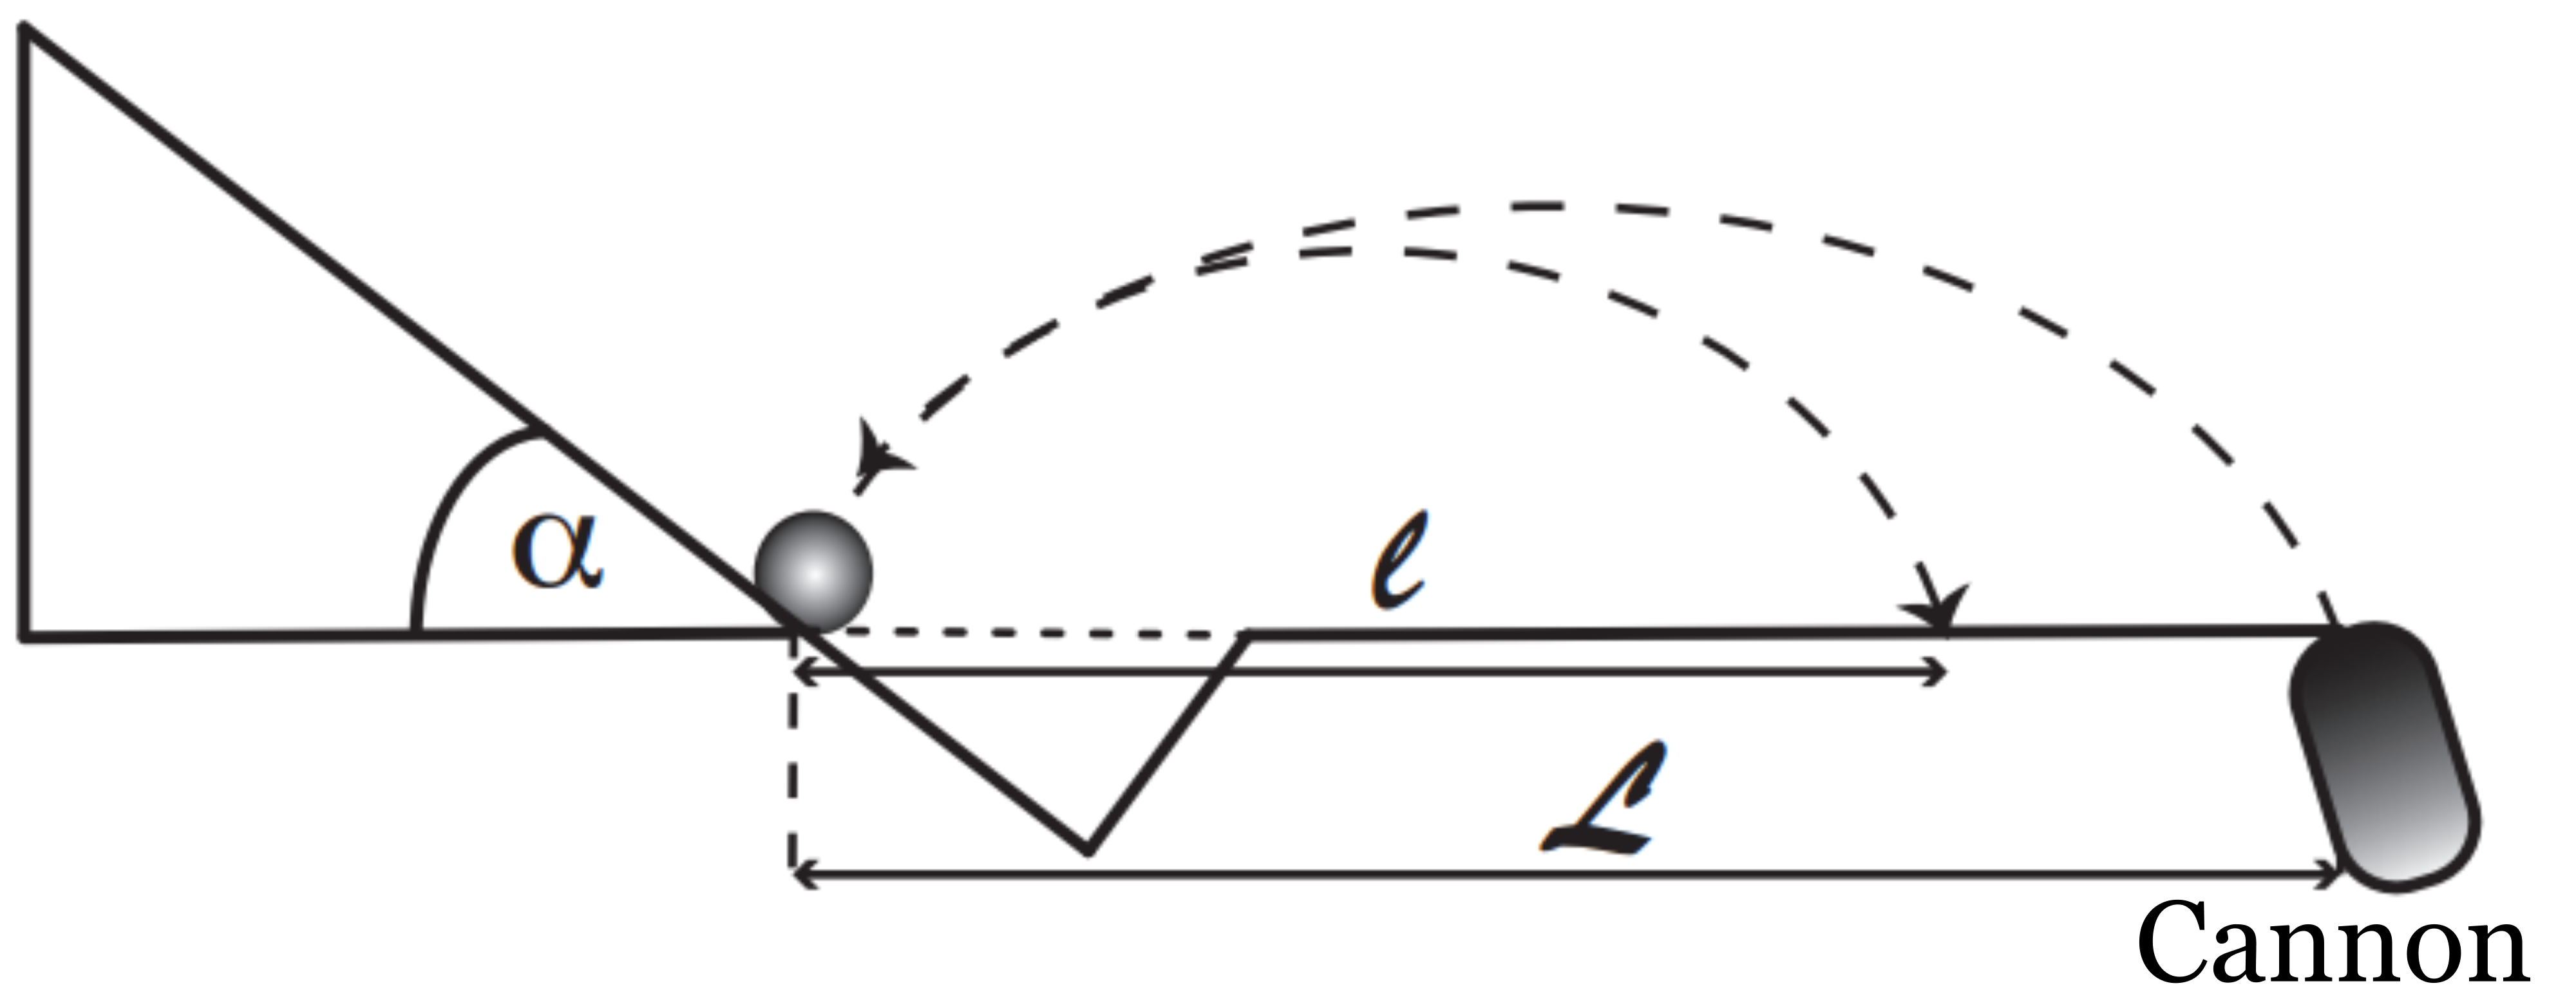
\includegraphics[width=0.5\textwidth]{2016-lahg-01-kaldjoonis_ing}
  \end{center}
  \vspace{-30pt}
\end{wrapfigure}
A rubber ball is fired out of a toy cannon so that the ball bounces perpendicularly to an inclined surface distanced horizontally $L$ from the cannon. The ball bounces off from the inclined surface to a distance $l$ (see figure). Find what fraction of the energy got absorbed during the bounce. The surface’s angle of inclination is $\alpha$.
\probend
\bigskip

% P11
\setAuthor{Oleg Košik}
\setRound{piirkonnavoor}
\setYear{2016}
\setNumber{G 2}
\setDifficulty{2}
\setTopic{Dünaamika}

\prob{Tug of war}
\probeng
Eero and Oleg compete in a tug of war so that during the whole competition the rope is horizontal. Eero’s mass is $m_1=\SI{110}{kg}$ and Oleg’s is $m_2=\SI{85}{kg}$. Coefficient of friction between the leg’s sole and floor $\mu=\SI{0,30}{}$ is same for both men. Which man wins? With what maximal acceleration can the winner force the loser to move, so that he himself stays put? The gravitational acceleration is $g=\SI{9,8}{m/s^2}$.
\probend
\bigskip

% P12
\setAuthor{Moorits Mihkel Muru}
\setRound{lõppvoor}
\setYear{2017}
\setNumber{G 1}
\setDifficulty{2}
\setTopic{Dünaamika}

\prob{Fastelavn slide}
\probeng
\begin{wrapfigure}[5]{r}{0.45\linewidth}
	\vspace{-5pt}
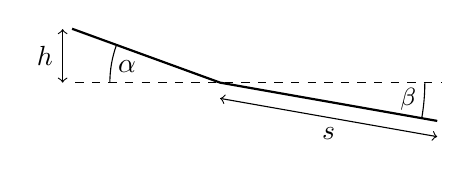
\begin{tikzpicture}[scale=0.4]
% Nõlv
\draw [thick] (0,0) -- (160:5);
\draw [thick] (0,0) -- (-10:7);

% Nurgad
\draw [dashed] (-4.6,0) -- (7,0);
\draw (160:3.5) arc (160:180:3.5) node at (170:3) {\(\alpha\)};
\draw (0:6.5) arc (0:-10:6.5) node at (-5:6) {\small\(\beta\)};

% Suurused
\draw [<->] (-5,0) -- (-5,1.7) node[pos=0.5, left] {\(h\)};
\draw [<->, yshift=-0.5cm] (0,0) -- (-10:7) node[pos=0.5, below] {\(s\)};	
\end{tikzpicture}
%\caption{Künka läbilõige} \label{liug}
\end{wrapfigure}
Juss found a hill for Fastelavn (a carnival tradition and holiday in Northern Europe) sliding. The hill’s cross-cut consists of two line segments, as shown in the figure. After the hill there is a horizontal ground. The height of the hill’s first part is \(h=\SI{2}{\meter}\) and its inclination is \(\alpha=\ang{20}\). The length of the second part is \(s=\SI{20}{\meter}\) and inclination \(\beta=\ang{5}\). The mass of Juss and the sledge is \(m=\SI{47}{\kilogram}\) and coefficient of friction between the snow and the sledge is \(\mu=\num{0.08}\), gravitational acceleration is \(g=\SI{9.8}{\meter\per\second\squared}\). Find how long is Juss’s slide.
\probend
\bigskip

% P13
\setAuthor{Kaur Aare Saar}
\setRound{lahtine}
\setYear{2013}
\setNumber{G 3}
\setDifficulty{3}
\setTopic{Dünaamika}

\prob{Alpinist}
\probeng
An alpinist with a mass of $m=\SI{75}{kg}$ is fastened to an elastic rope with a length of $L=\SI{6}{m}$. The other side of the rope is attached to a cliff. After climbing to a height of 6 meters from the attachment point the alpinist falls. Find the rope’s maximal elasticity coefficient $k$, knowing that a maximal pulling force of the rope that a human can tolerate is $T=25mg$. Do not account for air resistance.
\probend
\bigskip

% P14
\setAuthor{Taavi Pungas}
\setRound{piirkonnavoor}
\setYear{2014}
\setNumber{G 5}
\setDifficulty{3}
\setTopic{Dünaamika}

\prob{Parachute jump}
\probeng
Juku with a mass $m=\SI{60}{\kg}$ and his father Juhan with a mass $M=\SI{90}{\kg}$ decided to make a parachute jump. They put on the same parachutes with a mass of $m_v=\SI{10}{\kg}$ and then they were pushed off from the plane. Both of their parachutes opened at an exact same height $h$, after which the jumpers obtained a constant speed with negligible time and reached the ground with that speed. The time it took Juku to reach the ground from the point where he opened his parachute was $t=\SI{110}{\s}$. How much time $T$ did it take for Juhan? The drag force applied by the air to the parachute is proportional to the speed of falling squared. The air resistance applied to the jumpers themselves is negligible.
\probend
\bigskip

% P15
\setAuthor{Joonas Kalda}
\setRound{piirkonnavoor}
\setYear{2016}
\setNumber{G 4}
\setDifficulty{3}
\setTopic{Dünaamika}

\prob{Sledge}
\probeng
\begin{wrapfigure}[2]{r}{0.3\textwidth}
	\vspace{-12pt}
	\begin{resizebox}{\linewidth}{!}{
	\begin{tikzpicture}
	\coordinate (C) at (0.7,-0.1);
	\draw (0,0) -- ++(180-15:1.5);
	\draw (0,0) to [out = -15, in = 180] (C);
	\draw (C) to ++(0:1.5);
	\draw (180-15:1.5) -- ++(-15:0.2) -- ++(90-15:0.1) -- ++(180-15:0.2) -- (180-15:1.5);
	\end{tikzpicture}}
	\end{resizebox}
\end{wrapfigure}
Juku wants to cross an ice covered river on a sledge. He starts from a shore covered with snow, its slope has an angle of inclination $\alpha = 15^{\circ}$. The width of the river is $l = \SI{10}{m}$, coefficient of friction between the sledge and the snow is $\mu_1 = \SI{0.20}{}$ and between the sledge and the ice $\mu_2 = \SI{0.10}{}$. What must be the height of the shore with respect to the water’s surface so that Juku would slide to the other shore?
\probend
\bigskip

% P16
\setAuthor{Eero Vaher}
\setRound{lõppvoor}
\setYear{2016}
\setNumber{G 2}
\setDifficulty{3}
\setTopic{Dünaamika}

\prob{Car’s braking}
\probeng
A car is driving on a road, the road’s change of height per toad length is $k=\frac{1}{30}$. With a same initial speed and braking force the car stops during a distance $s_1=\SI{25}{m}$ while driving uphill, while downhills during a distance $s_2=\SI{30}{m}$. What is the value of the car’s initials speed $v$? Gravitational acceleration is $g=\SI{9.8}{\meter\per\second\squared}$.
\probend
\bigskip

% P17
\setAuthor{Hans Daniel Kaimre}
\setRound{lõppvoor}
\setYear{2016}
\setNumber{G 3}
\setDifficulty{3}
\setTopic{Dünaamika}

\prob{Cannonball}
\probeng
Juku calculated during a school lesson that the maximal height of a cannonball that is shot from a very powerful cannon is $H=\SI{400}{\km}$. But he did not consider that at those heights the gravitational field’s change is significant and that the gravity force cannot be assumed to be constant. Find how high the ball would actually fly. Earth’s radius is $R=\SI{6400}{\km}$. Do not account for air resistance.
\probend
\bigskip

% P18
\setAuthor{Andreas Valdmann}
\setRound{piirkonnavoor}
\setYear{2017}
\setNumber{G 3}
\setDifficulty{3}
\setTopic{Dünaamika}

\prob{Pendulum}
\probeng
A pendulum made from a string and a weight is swinging so that at the amplitude position the angle between the string and the vertical direction is $\alpha=\ang{60}$. How many times do the maximal and minimal tensions differ in the string during the swinging?
\probend
\bigskip

% P19
\setAuthor{Jonatan Kalmus}
\setRound{lõppvoor}
\setYear{2017}
\setNumber{G 2}
\setDifficulty{3}
\setTopic{Dünaamika}

\prob{Mountain’s slope}
\probeng
What is the maximal angle of inclination $\alpha$ of a mountain so that it is possible to drive on it upwards with a bicycle while maintaining a constant speed? The mass of a cyclist is $m$, bicycle’s mass is $M$, pedal’s crank length is $r_1$, the front gear wheel’s radius is $r_2$, rear gear wheel’s radius is $r_3$, radius of the wheel is $r_4$. Assume that during the cycling the cyclist’s center of mass is still with respect to the bicycle and that all of the cyclist’s mass is applied to a sinking pedal. Coefficient of friction between the ground and the wheel is big enough to avoid sliding. Do not account for mechanical friction during the force transmission and the coefficient of rolling resistance is negligible. Assume that the average speed of the bicycle is constant and that the relative change in speed is negligible during a quarter of pedaling period.\\
\emph{Note}. The problem’s text has been adjusted compared to the version that appeared in the olympiad.
\probend
\bigskip

% P20
\setAuthor{Kristian Kuppart}
\setRound{lahtine}
\setYear{2011}
\setNumber{G 3}
\setDifficulty{4}
\setTopic{Dünaamika}

\prob{Truck}
\probeng
There is a liquid in a truck’s crate of height $H$, the liquid’s surface height from the crate’s bottom is $h$, moreover $h > \frac{H}{2}$. What can the truck’s maximal acceleration $a$ be, so that the liquid will not flow out of the crate? The length of the truck’s crate is $L$.\\
\emph{Note}. The truck is accelerating uniformly, thanks to that the liquid is not going to sway.
\probend
\bigskip

% P21
\setAuthor{Andreas Valdmann}
\setRound{piirkonnavoor}
\setYear{2012}
\setNumber{G 5}
\setDifficulty{4}
\setTopic{Dünaamika}

\prob{Loop-the-loop track}
\probeng
\begin{wrapfigure}{r}{42mm}%
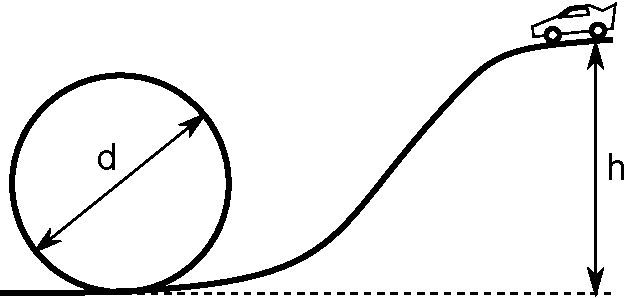
\includegraphics[width=\linewidth]{2012-v2g-05-silmus}%
\end{wrapfigure}
A toy car’s track is shown in the figure. The car begins from a resting position on top of the inclined track. The car accelerates while driving down and finally drives through a loop. What is the minimal height $h$ so that the car will not drop down while driving through the loop? The loop’s diameter is $d$. Do not account for friction.
\probend
\bigskip

% P22
\setAuthor{Mihkel Kree}
\setRound{lõppvoor}
\setYear{2012}
\setNumber{G 2}
\setDifficulty{4}
\setTopic{Dünaamika}

\prob{Water spurt}
\probeng
In the figure below there is a photo of a water spurt flowing out of a horizontal tube and a coordinate grid, the grid’s smallest unit is equal to the water spurt’s diameter on its initial height. A measuring cup of volume $V=\SI{150}{cm^3}$ is placed below the spurt, which is flowing with even speed.  It takes $t=\SI{5}{min}$ for the cup to fill completely. Find the tube’s inner diameter.
\begin{center}
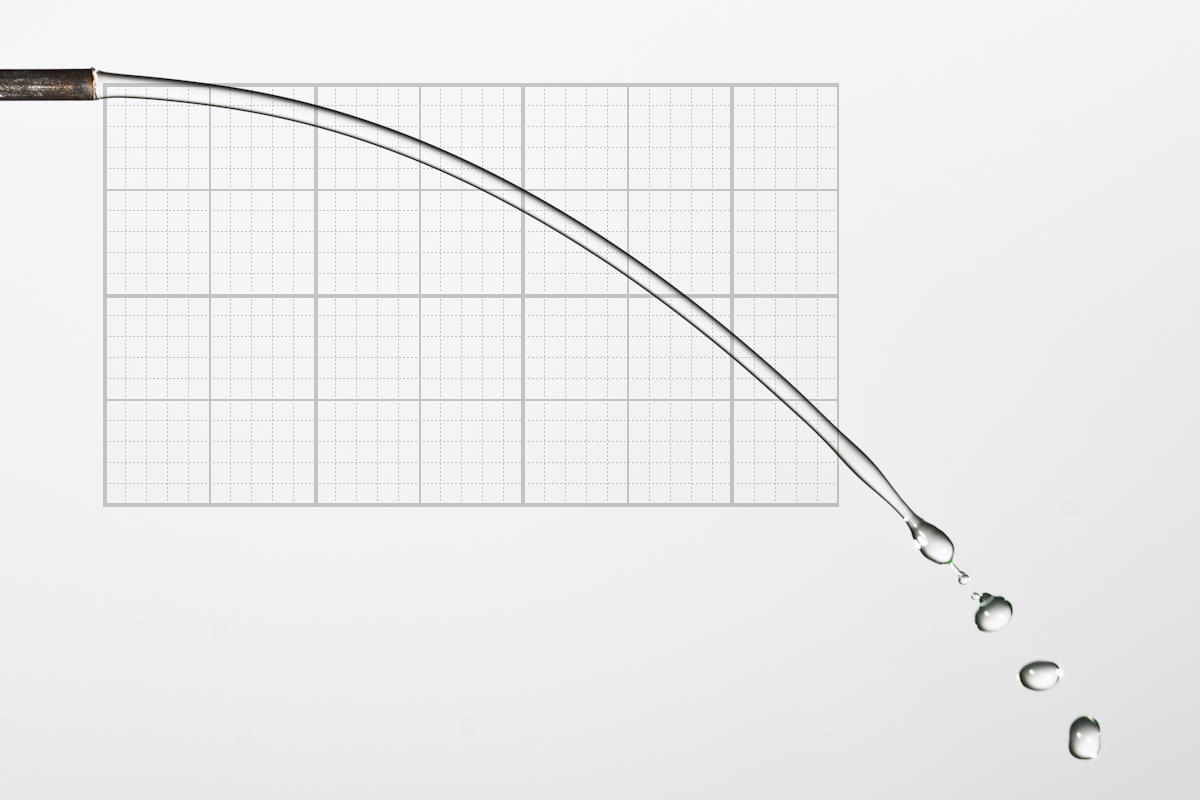
\includegraphics[width=0.7\linewidth]{2012-v3g-02-jet}%
\end{center}
\probend
\bigskip

% P23
\setAuthor{Aigar Vaigu}
\setRound{piirkonnavoor}
\setYear{2016}
\setNumber{G 6}
\setDifficulty{4}
\setTopic{Dünaamika}

\prob{Shooting range}
\probeng
In an indoors shooting range a target is shot at with a rifle, the speed of the rifle’s bullet is $v=\SI{320}{m/s}$ and the target is at a distance $s=\SI{30}{m}$. The shooter is aiming the rifle at the target which is at the same height as the rifle and shoots the target exactly in the middle. Evaluate how far from the target would the bullet land if the rifle is turned 180 degrees around the aiming axis. Do not account for air resistance.
\probend
\bigskip

% P24
\setAuthor{Kaur Aare Saar}
\setRound{lõppvoor}
\setYear{2016}
\setNumber{G 4}
\setDifficulty{4}
\setTopic{Dünaamika}

\prob{Cylinder}
\probeng
A cylinder of mass $m$ and radius $R$ is sliding on a plane with a speed $v$ and an angular velocity $\omega$. When the sliding ends the cylinder moves with the speed $v$ to the opposite direction with respect to the initial speed. Find the cylinder’s initial angular velocity.
\begin{center}
	\begin{resizebox}{0.35\linewidth}{!}{
			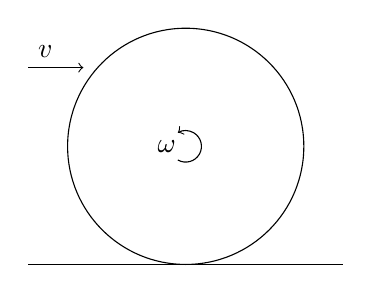
\begin{tikzpicture}
			\draw (0,2.5) node[anchor=south west] {$v$};
			\draw[->] (0,2.5) -- ++(0:0.7);
			\draw (0,0) --(4,0);
			\draw (2,1.5) circle (1.5);
			\draw [->] (2,1.5) node[anchor = east] {$\omega$} ++(-120:0.2) arc (-120:120:0.2);
			\end{tikzpicture}}
	\end{resizebox}
\end{center}
\probend
\bigskip

% P25
\setAuthor{Jonatan Kalmus}
\setRound{piirkonnavoor}
\setYear{2018}
\setNumber{G 5}
\setDifficulty{4}
\setTopic{Dünaamika}

\prob{Truck on a roundabout}
\probeng
A truck is driving with a uniform speed on a roundabout of radius $R$. Find the truck’s maximal possible speed provided that the coefficient of friction is big enough to avoid sliding. The truck’s center of mass is at a height $h$ from the ground and the truck’s width is $l$. Gravitational acceleration is $g$.
\probend
\bigskip

% P26
\setAuthor{Ants Remm}
\setRound{lahtine}
\setYear{2012}
\setNumber{G 6}
\setDifficulty{5}
\setTopic{Dünaamika}

\prob{Chlorine’s molecule}
\probeng
Chlorine’s molecule, which is moving with a velocity $v = \SI{600}{m/s}$, absorbs a photon with a wavelength $\lambda = \SI{350}{nm}$ and is divided into two atoms. The first atom’s velocity is measured to be $ u = \SI{1600}{m/s}$, which perpendicular to the molecule’s initial velocity. Find the chlorine molecule’s binding energy if all the particles were at a state with minimal inner energy. Planck constant is $h =
\SI{6,6e-34}{J.s}$, speed of light is $c = \SI{3,0e8}{m/s}$, chlorine’s atomic number is 35 and Avogadro constant is $N_A
= \SI{6,0e23}{\text{mol}^{-1}}$. Photon’s energy is defined as $E =
\frac{h c}{\lambda}$. It is presumed that a photon’s momentum is negligible compared to chlorine’s momentum.
\probend
\bigskip

% P27
\setAuthor{Andres Põldaru}
\setRound{lahtine}
\setYear{2014}
\setNumber{G 5}
\setDifficulty{5}
\setTopic{Dünaamika}

\prob{Swing}
\probeng
On one end of the swing at a length $l_1$ from the swing’s rotation axis there is a mass $m_1$. On the other end of the swing, which is $l_2$ away from the rotation axis, falls a mass $m_2$ from a height $h$. The collision is completely inelastic and the swing is horizontal at the moment of collision. The swing’s mass is very small and it does not have to be taken into account. How fast does the first mass move right after the collision?
\probend
\bigskip

% P28
\setAuthor{Jaan Toots}
\setRound{lahtine}
\setYear{2015}
\setNumber{G 6}
\setDifficulty{5}
\setTopic{Dünaamika}

\prob{Hydrogen’s ionization}
\probeng
What is the smallest kinetic energy $K_0$ of a free proton that is able to ionize a hydrogen atom? Assume that the electron inside the hydrogen atom is still and that the electromagnetic interaction between the atomic nucleus and the free proton is negligible. Hydrogen’s binding energy is $E_0 = \SI{13.6}{\electronvolt}$, proton’s mass is $m_p=\SI{1.67e-27}{kg}$ and electron’s mass $m_e=\SI{9.11e-31}{kg}$.
\probend
\bigskip

% P29
\setAuthor{Kristian Kuppart}
\setRound{piirkonnavoor}
\setYear{2015}
\setNumber{G 5}
\setDifficulty{5}
\setTopic{Dünaamika}

\prob{Water pipe}
\probeng
\begin{wrapfigure}[7]{r}{0.15\textwidth}
  \vspace{-35pt}
  \begin{center}
    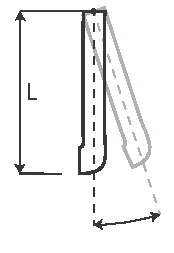
\includegraphics[width=0.18\textwidth]{2015-v2g-05-toru}
  \end{center}
  \vspace*{-10pt}
\end{wrapfigure}
A water pipe with a length $L$ is fixed to a wall so that it can freely rotate on the vertical plane. The water pipe’s mass together with the water it is filled with is $M$. The cross-sectional area of the pipe’s end is $S$. The end is turned 90 degrees with respect to the rest of the pipe (see figure). Water flows out of the end of the pipe with a speed $v$ and density $\rho$. What is the angle between the vertical direction and the pipe’s axis? Gravitational acceleration is $g$.
\probend
\bigskip

% P30
\setAuthor{Mihkel Kree}
\setRound{piirkonnavoor}
\setYear{2015}
\setNumber{G 6}
\setDifficulty{5}
\setTopic{Dünaamika}

\prob{Collision}
\probeng
\begin{wrapfigure}{l}{0.22\textwidth}
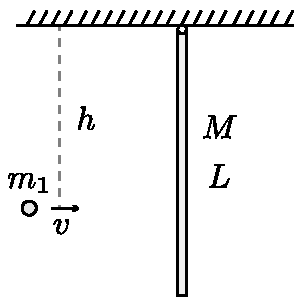
\includegraphics[width=0.22\textwidth]{2015-v2g-06-porgejoonis}
\end{wrapfigure}
An initially resting rod of mass $M$ and length $L$ is hanging from the ceiling so that its upper tip is fixed with a freely rotating attachment. The rod’s moment of inertia with respect to the tip is $I=\frac{1}{3}ML^2$. A steel ball with a mass $m_1$ flies against the rod and hits it at a distance $h$ from the fixed tip. The collision is elastic, which means there is no heat loss. Interestingly, the ball stays put for a moment after the collision and then starts to fall down vertically. Find the value of $h$ so that such a moment of stillness is possible.
\probend
\bigskip

% P31
\setAuthor{Ardi Loot}
\setRound{lahtine}
\setYear{2016}
\setNumber{G 6}
\setDifficulty{5}
\setTopic{Dünaamika}

\prob{Cyclist}
\probeng
A cyclist with a mass $m=\SI{100}{kg}$ rides without pedaling down a hill with an angle of inclination of $\theta_{1}=\ang{4.8}$ (angle between the horizontal and the hill) and notices that if the hill is long enough his final speed would be $v_{1}=\SI{50}{km/h}$. However, if the mountain is two times smaller $(\theta_{2}=\ang{2.4})$ his final speed would be smaller by $\Delta v=\SI{15}{km/h}$. Find how big must be the cyclist pedaling power so he would maintain a speed of $v=\SI{20}{km/h}.$ on a horizontal road. What fraction of the power does it take to overcome the air resistance? Assume that there is a windless weather and that the gravitational acceleration is $g=\SI{9.8}{m/s^{2}}$. \\
\emph{Note.} You should take into account the friction force that does not depend on the speed and also the wind resistance which is proportional to speed squared.
\probend
\bigskip

% P32
\setAuthor{Rasmus Kisel}
\setRound{piirkonnavoor}
\setYear{2017}
\setNumber{G 7}
\setDifficulty{5}
\setTopic{Dünaamika}

\prob{Two balls and a spring}
\probeng
Small balls are fixed to both ends of a spring, the first ball’s mass is $M$ and the mass of the other one is unknown. The whole system is made to rotate so that the distance of the unknown mass from the rotation center is equal to the spring’s initial length. What is the period of such a rotation if the spring’s stiffness is $k$? The spring’s mass is negligible with respect to the masses of the balls.
\probend
\bigskip

% P33
\setAuthor{Moorits Mihkel Muru}
\setRound{lõppvoor}
\setYear{2017}
\setNumber{G 5}
\setDifficulty{5}
\setTopic{Dünaamika}

\prob{Passenger train}
\probeng
A passenger train drives on a railway’s circular arc-shaped section while slowing down evenly. The length of the section is $s$ and the time it takes the train to drive through it is $t$. After driving through the section the train’s direction has changed by an angle $\varphi$ and at the beginning of the section the train’s speed was $\alpha$ times bigger than it was at the end of the section. Find the relationship between the mass $m$ of a passenger sitting in the train and the passenger’s weight $P$ at the moment when the train is in the midpoint of the section. Find the passenger’s mass if $P=\SI{840}{\newton}$, $s=\SI{1.5}{\kilo\meter}$, $t=\SI{60}{\second}$, $\alpha=\num{1.5}$, $\varphi=\ang{60}$ and $g=\SI{9.8}{\meter\per\second\squared}$.
\probend
\bigskip

% P34
\setAuthor{Hans Daniel Kaimre}
\setRound{lõppvoor}
\setYear{2018}
\setNumber{G 4}
\setDifficulty{5}
\setTopic{Dünaamika}

\prob{Pendulum with two parts}
\probeng
\begin{wrapfigure}[10]{r}{0.4\textwidth}
\vspace{-5pt}
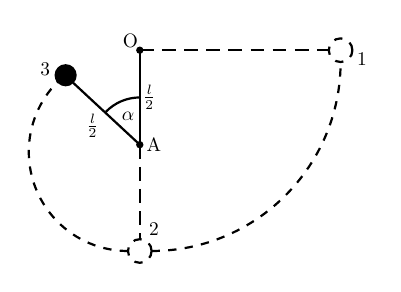
\begin{tikzpicture}[thick,scale=0.6, every node/.style={scale=0.7}]

    % Def. koordinaadid
    \coordinate (O) at (0,0) ;
    \coordinate (1) at (4,0) ;
    \coordinate (A) at (0,-2) ;
    \coordinate (2) at (0,-4);
    \coordinate (3) at (-1.41,-0.69);

    % Jooned, t2pid
    \draw[dash pattern=on5pt off3pt] (O) -- (1);
    \draw[dash pattern=on5pt off3pt] (A) -- (2);
    \draw[thick,dashed] (4.25,0) circle (0.25cm);
    \draw[thick,dashed] (0,-4.25) circle (0.25cm);
    \draw[thick] (O) -- (A);
    \draw[thick] (A) -- (3);
    \filldraw [black] (A) circle (1.5pt);
    \filldraw [black] (O) circle (1.5pt);
    \filldraw [black] (-1.57,-0.53) circle (6pt);
    
    

    % Nurgad ja punktid
    \draw (0,-1) arc (90:136:1);
    \draw[thick, dashed] (0.25,-4.25) arc (270:360:4);
    \draw[thick, dashed] (-0.25,-4.25) arc (270:135:2.1);
    \node[] at (-0.25,-1.4)  {$\alpha$};
    \node[] at (4.7,-0.2)  {$1$};
    \node[] at (0.3,-3.8)  {$2$};
    \node[] at (-2.0,-0.4)  {$3$};
    \node[] at (-0.2,0.2)  {O};
    \node[] at (0.3,-2)  {A};
    \node[] at (0.2,-1)  {$\frac{l}{2}$};
    \node[] at (-1,-1.6)  {$\frac{l}{2}$};
\end{tikzpicture}
\end{wrapfigure}
A thread of length $l$ is fixed to a point O and a small ball is hanging at the end of the thread. The ball is brought to the side and is released at the position 1 without additional force. When the ball reaches the position 2 the thread meets a rod at the point A, the rod is perpendicular to the drawing’s plane. In the same vertical the point A is at a length $l/2$ from the point O. Find for what value of $\alpha$ is the thread’s tension $T=0$ (position 3). Do not account for air resistance or friction.
\probend
\bigskip

% P35
\setAuthor{Hans Daniel Kaimre}
\setRound{piirkonnavoor}
\setYear{2016}
\setNumber{G 8}
\setDifficulty{6}
\setTopic{Dünaamika}

\prob{Rolling ball}
\probeng
\begin{wrapfigure}{r}{0.35\textwidth}
	\vspace{-10pt}
	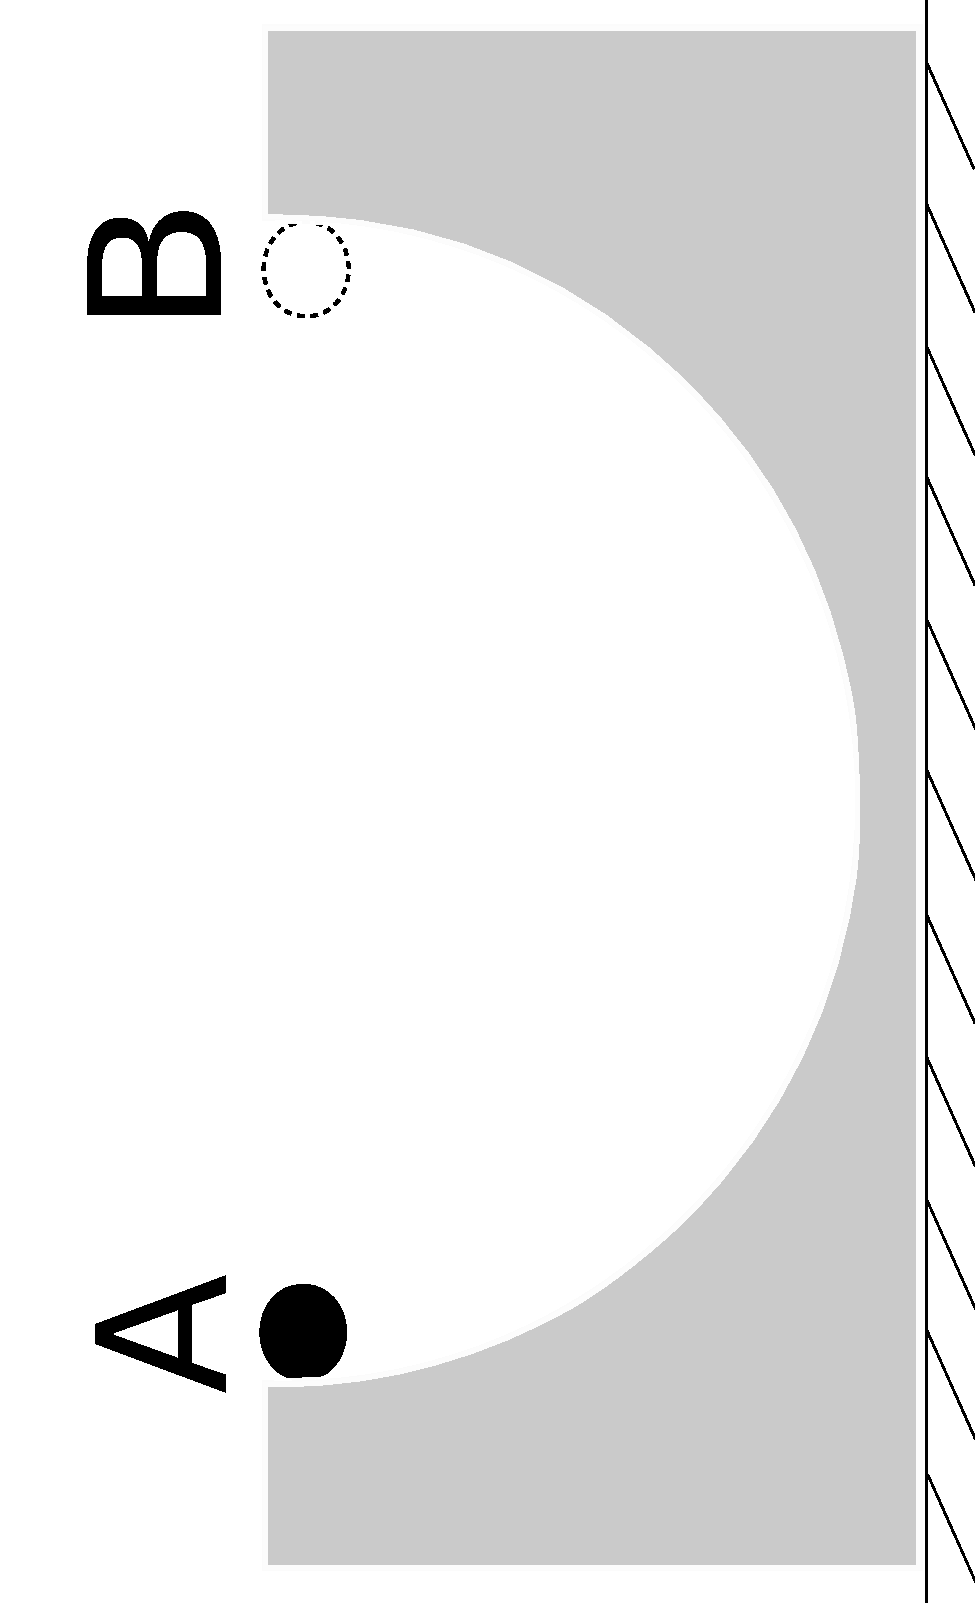
\includegraphics[angle=-90,origin=c,width=0.4\textwidth]{2016-v2g-08-halfpipe}
	\vspace{-60pt}
\end{wrapfigure}
A semi-cylindrical piece of radius $R$ is cut out from a tile. The tile is standing on a smooth frictionless horizontal surface (see figure). The tile’s mass is $M$. A small ball of radius $r$ and mass $m$ is pushed down from the point A to move along the cylindrical surface. How much has the tile moved by the moment when the ball reaches the point B?
\probend
\bigskip

% P36
\setAuthor{Tanel Kiis}
\setRound{lahtine}
\setYear{2012}
\setNumber{G 7}
\setDifficulty{7}
\setTopic{Dünaamika}

\prob{Braking}
\probeng
A body of mass $M$ falls freely with an acceleration $g$. Trying to change its speed, someone fires small balls of mass $m$ directly up from the ground after each $t$ seconds. The balls bounce elastically directly back. How big has to be the speed $u$ of the balls so that after each collision the speed of the falling body is exactly the same, $v$? You can assume that the change in the speed of the balls is negligible under gravitation and that $m\ll M$.
\probend
\bigskip

% P37
\setAuthor{Madis Ollikainen}
\setRound{piirkonnavoor}
\setYear{2012}
\setNumber{G 9}
\setDifficulty{7}
\setTopic{Dünaamika}

\prob{Robin Hood}
\probeng
Robin Hood is in an archery competition where he has to hit a target at a distance $L=\SI{200}{m}$. At what angle $\alpha$ with respect to the horizontal direction has to Robin shoot with his bow so he would hit the target exactly in the middle? While straining the bow Robin’s work is $A=\SI{500}{J}$ and the bow’s coefficient of efficiency is $\eta=0,17$. The arrow’s mass is $m=\SI{54}{g}$ and it is shot $h=\SI{70}{cm}$ higher than the target’s center is. Do not account for air resistance. Gravitational acceleration is $g=\SI{9,8}{m/s^2}$.
\probend
\bigskip

% P38
\setAuthor{Mihkel Rähn}
\setRound{lõppvoor}
\setYear{2014}
\setNumber{G 7}
\setDifficulty{7}
\setTopic{Dünaamika}

\prob{Sports car}
\probeng
Find the maximal acceleration of a front-wheel drive car. The car’s mass is $m$, the distance between the axes of the front and rear wheels is $b$, the center of mass is at a height $h$ and the horizontal distance of the center of mass from the rear axis is $s$. Coefficient of friction between the wheels and the ground is $\mu$.
\probend
\bigskip

% P39
\setAuthor{Kaur Aare Saar}
\setRound{lahtine}
\setYear{2015}
\setNumber{G 8}
\setDifficulty{7}
\setTopic{Dünaamika}

\prob{Slat}
\probeng
A long slat that is lying on a horizontal plane is pushed from one end with a constant speed, perpendicularly to the slat. How far from that slat’s end is the rotation axis of the slat? The length of the slat is $L$. Coefficient of friction between the slat and the plane is the same everywhere.
\probend
\bigskip

% P40
\setAuthor{Tanel Kiis}
\setRound{piirkonnavoor}
\setYear{2013}
\setNumber{G 9}
\setDifficulty{8}
\setTopic{Dünaamika}

\prob{Hollow ball}
\probeng
Juku has an iron ball ($\varrho_\mathrm{Fe}=\SI{7,9}{\gram\per\centi\meter\cubed}$) of radius $r=\SI{10}{\centi\meter}$ and mass $m=\SI{30}{\kilo\gram}$. Juku knows that inside the ball there is a spherical hollowness and he wants to find the distance $d$ from the center of the ball to the center of the hollowness. To do that he hanged the ball to a thread two times, using two opposite points on the ball as the hanging points. At the first time, the axis that connected the two hanging points formed an angle $\alpha=\ang{60}$ with respect to the horizontal axis, the second time that angle was $\beta=\ang{45}$. Find $d$.
\probend
\bigskip

% P41
\setAuthor{Andreas Valdmann}
\setRound{lõppvoor}
\setYear{2013}
\setNumber{G 9}
\setDifficulty{8}
\setTopic{Dünaamika}

\prob{Football players}
\probeng
Two football players tried a trick move, where two balls would collide in the air. The players stood from each other at a distance $d = \SI{20}{m}$ and hit their balls at the same time, both giving the ball an initial speed of $v = \SI{15}{m/s}$. In what area could the balls collide during the flight? To answer, make a figure from top view where the locations of the players are marked and the area of all the possible collision points. Also give the dimensions of that area. You do not have to find at what height from the ground the possible collision points are. Gravitational acceleration is $g = \SI{9,8}{m/s^2}$.
\probend
\bigskip

% P42
\setAuthor{Andres Põldaru}
\setRound{lahtine}
\setYear{2015}
\setNumber{G 9}
\setDifficulty{8}
\setTopic{Dünaamika}

\prob{Wrench}
\probeng
Let us take a look at a wrench that can be regulated. How big has to be the number of its grooves per unit of length, $n$, so that the nuts can be firmly fixed? The coefficient of friction between the touching surfaces is $\mu$ and the radius from the regulator’s axis to the touching surfaces is $r$.
\begin{center}%
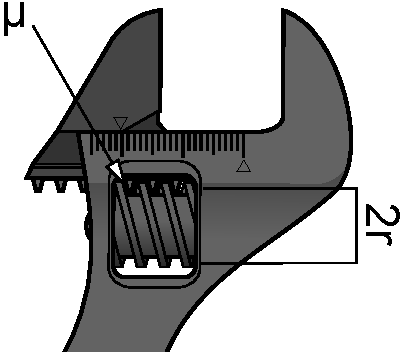
\includegraphics[width=0.4\linewidth]{2015-lahg-09-mutriv6ti_joonis}%
\end{center}
\probend
\bigskip

% P43
\setAuthor{Taavet Kalda}
\setRound{lahtine}
\setYear{2017}
\setNumber{G 8}
\setDifficulty{8}
\setTopic{Dünaamika}

\prob{Blocks}
\probeng
In the figure there is depicted a system that consists of two blocks and three weights of masses $m_1$, $m_2$ and $M$. The strings are non-stretchable and the masses of the strings and blocks are insignificant compared to the masses of the weights. The friction between a block and a string is insignificantly small. What has to be the value of $M$ so that $M$ would initially stay still when the system is let free?
\begin{center}
	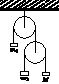
\includegraphics[width = 0.3\linewidth]  {2017-lahg-08-double_pulleys_img.pdf}
\end{center}
\probend
\bigskip

% P44
\setAuthor{Jaan Kalda}
\setRound{lahtine}
\setYear{2017}
\setNumber{G 9}
\setDifficulty{8}
\setTopic{Dünaamika}

\prob{Toy car}
\probeng
The distance between a toy car’s axes is $L$, the center of mass is equally distanced from the axes and it is at a height $h$ from the horizontal plane. The front wheels of the car can freely turn and their masses are insignificant. The rear wheels, however, do not turn at all. The car is lying on a horizontal plane, the coefficient of friction between the wheel and the horizontal plane is $\mu$ and the gravitational acceleration is $g$.\\
The horizontal plane starts to move back and forth with a high frequency. At the first half-period the surface’s velocity vector is directed from the car’s rear wheel towards the front wheel and at the second half-period the direction is the opposite; during both of the half-periods the speed stays constant; during the oscillation the surface is moved so fast that the car always slides either one way or another with respect to the surface. With what average acceleration does the car start to move?
\probend
\bigskip

% P45
\setAuthor{Jaan Kalda}
\setRound{lahtine}
\setYear{2012}
\setNumber{G 10}
\setDifficulty{9}
\setTopic{Dünaamika}

\prob{Fragments}
\probeng
A clay ball of mass 10 g fell vertically down to a smooth horizontal ground and broke into three fragments. The fragments scattered on the ground and stopped at points that are given in the figure (top view, the cross represents the falling point). Find the masses of the fragments. You can make additional designs on the drawing (on a separate paper) and take additional measurements. You can assume that the fragments started to slide right after the fall without bouncing upwards, the air friction is insignificant and that the coefficient of kinetic friction does not depend on the speed. 
\begin{center}
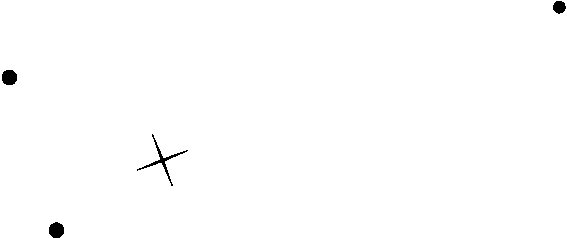
\includegraphics[width=0.8\linewidth]{2012-lahg-10-killud}
\end{center}
\probend
\bigskip

% P46
\setAuthor{Roland Matt}
\setRound{lõppvoor}
\setYear{2012}
\setNumber{G 8}
\setDifficulty{9}
\setTopic{Dünaamika}

\prob{Hourglass}
\probeng
Let us study an hourglass model. The hourglass consists of a cylindrical tube of length $L$, the tube is separated with a plate in the middle and the plate is evenly covered with holes. The sand can flow through these holes. In a good approximation the mass flow rate $w$ of the sand flowing through the holes does not depend on the amount of sand in the upper part of the tube. The hourglass is put on a scale while the sand is flowing and again when the sand has flown down. What is the difference between the scale readings? The sand’s density is $\rho$ and the area of the tube’s cross section is $S$. Assume that the mass of the falling sand is insignificant compared to the sand’s whole mass.
\probend
\bigskip

% P47
\setAuthor{Jaan Kalda}
\setRound{lõppvoor}
\setYear{2014}
\setNumber{G 8}
\setDifficulty{9}
\setTopic{Dünaamika}

\prob{Cylindrical vessels}
\probeng
\begin{wrapfigure}{r}{0.06\textwidth}%
\vspace{-15pt}
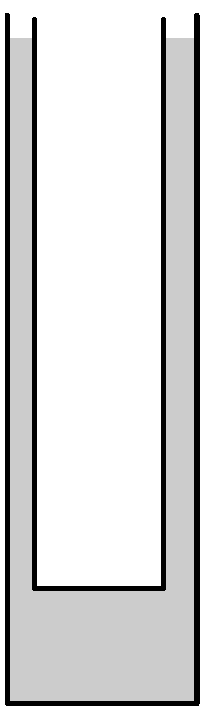
\includegraphics[width=0.06\textwidth]{2014-v3g-08-cylinders}
\end{wrapfigure}
A cylindrical vessel of inside radius $R = \SI{30}{mm}$ is filled with water. Another empty cylindrical vessel of radius $r =\SI{25}{mm}$ and with an insignificantly small mass is coaxially pressed into the bigger cylinder so that the length of the part in the water is $L = \SI{300}{mm}$ (see figure). Find the acceleration of the inner cylinder right after when it is let free. You do not have to account for the water’s surface tension or viscosity.
\probend
\bigskip

% P48
\setAuthor{Mihkel Kree}
\setRound{lõppvoor}
\setYear{2015}
\setNumber{G 8}
\setDifficulty{9}
\setTopic{Dünaamika}

\prob{Spring}
\probeng
In a box there is a weight fixed to a spring. Both the box and the weight have a mass $m$. The mass of the spring is insignificantly small and its stiffness is $k$. The box is dropped down freely from a height $h$ so that during the falling the weight is in an equilibrium state. Colliding with a soft surface the box stays still for a moment. The box is high enough for the weight not to collide against the box. Not for one moment is the spring completely pressed together.\\
\osa What is the smallest dropping height $h_\text{m}$ for the box to jump back up again?\\
\osa The box was dropped from a height $h\approx h_\text{m}$ found in the section a). For what time $t$ will the box be on the ground before starting to rise up?\\
\emph{Note.} Notice that during a free fall the mass inside the box is in a weightless state and because of that the spring is not stretched out during the fall. When reaching the ground the weight is not in the equilibrium position anymore and because of that starts to swing around a new equilibrium position with an angular frequency of $\omega =\sqrt{\frac{k}{m}}$.
\probend
\bigskip

% P49
\setAuthor{Jaan Kalda}
\setRound{lahtine}
\setYear{2017}
\setNumber{G 10}
\setDifficulty{9}
\setTopic{Dünaamika}

\prob{Rods}
\probeng
\begin{wrapfigure}[7]{r}{0.4\textwidth}
	\vspace{-10pt}
	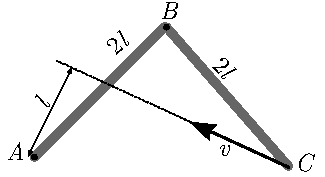
\includegraphics[width = 0.4\textwidth]  {2017-lahg-10-delta.pdf}
\end{wrapfigure}
In the given figure a hinged construction is pictured, it consists of two rods with a length $2l$. One of the rod’s tip is fixed to an unmoving point $A$ and the other rod’s tip $C$ moves with a constant velocity $v$ along a direction which passes the point $A$ at the distance $l$. Find the acceleration of the connection point $B$ of the rods during the moment when the distance between the points $A$ and $C$ is $2l$.
\probend
\bigskip
\newpage\subsection{\protect\StrSubstitute{Electric circuits}{-}{ }}

% P50
\setAuthor{Eero Vaher}
\setRound{piirkonnavoor}
\setYear{2016}
\setNumber{G 1}
\setDifficulty{1}
\setTopic{Elektriahelad}

\prob{Voltmeters}
\probeng
In a circuit diagram there is a voltage source of voltage $U_0=\SI{30}{V}$ and four identical voltmeters. What is the reading of each voltmeter?
\begin{center}
	\tikzset{component/.style={draw,thick,circle,fill=white,minimum size =0.75cm,inner sep=0pt}}
	\begin{resizebox}{0.45\linewidth}{!}{
		\begin{circuitikz}
			\draw
			
			(6,0) to[battery1,l=${U_0=\SI{30}{V}}$] (0,0) to (0,2) to (6,2) to (6,0)
			(2,2) to[short, *-] (2,3) to (6,3) to[short, -*] (6,2)
			;
			\node[component] at (1,2) {V$_1$};
			\node[component] at (3,2) {V$_2$};
			\node[component] at (5,2) {V$_3$};
			\node[component] at (4,3) {V$_4$};
		\end{circuitikz}}
	\end{resizebox}
\end{center}
\probend
\bigskip

% P51
\setAuthor{Erkki Tempel}
\setRound{piirkonnavoor}
\setYear{2017}
\setNumber{G 1}
\setDifficulty{1}
\setTopic{Elektriahelad}

\prob{Voltmeter}
\probeng
In the circuit diagram pictured below there is an ideal ammeter which shows a current $I$. The ammeter is replaced by an ideal voltmeter. How big is the voltmeter’s reading? The resistance of all the resistors is $R$.
\begin{center}
	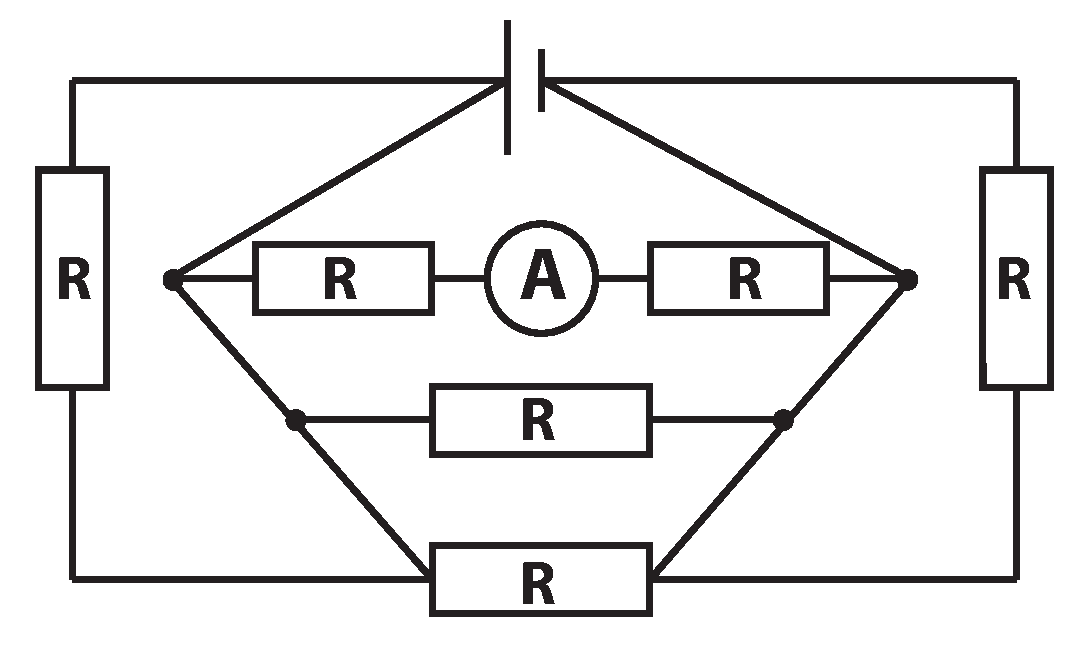
\includegraphics[width=0.4\textwidth]{2017-v2g-01-skeem}
\end{center}
\probend
\bigskip

% P52
\setAuthor{Mihkel Kree}
\setRound{piirkonnavoor}
\setYear{2015}
\setNumber{G 2}
\setDifficulty{2}
\setTopic{Elektriahelad}

\prob{Lamps}
\probeng
A voltage source is connected in parallel with two lamps, one of the lamps is lit with $k$ times bigger power than the other. Next these lamps are connected in series with the same voltage source. How many times does the total power dissipated by the lamps change? Will it be smaller or bigger?
\probend
\bigskip

% P53
\setAuthor{Oleg Košik}
\setRound{piirkonnavoor}
\setYear{2013}
\setNumber{G 5}
\setDifficulty{3}
\setTopic{Elektriahelad}

\prob{Circuit diagram}
\probeng
\begin{wrapfigure}[7]{r}{2.5cm}%
\vspace{-15pt}
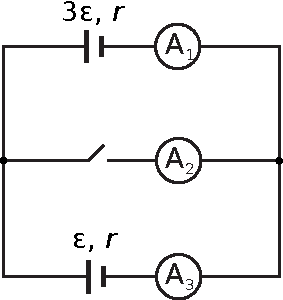
\includegraphics[width=\linewidth]{2013-v2g-05-skeem}%
\end{wrapfigure}
The ammeters in the circuit diagram given in the drawing are ideal; the electromotive forces and internal resistances of the batteries are marked in the drawing. Find the readings of the ammeters if\\
a) the switch is closed;\\
b) the switch is opened. (\emph{Note.}  In practice this circuit should be used only when it is certain that the appearing currents will stay in the regions measured by the ammeters!)
\probend
\bigskip

% P54
\setAuthor{Eero Vaher}
\setRound{lahtine}
\setYear{2014}
\setNumber{G 4}
\setDifficulty{3}
\setTopic{Elektriahelad}

\prob{Tetrahedron}
\probeng
A tetrahedron’s (a pyramid made of four equilateral triangles) edges are identical resistors with a resistance $R$. Find the resistance between the tetrahedron’s two tips.
\probend
\bigskip

% P55
\setAuthor{Taavi Pungas}
\setRound{lõppvoor}
\setYear{2014}
\setNumber{G 1}
\setDifficulty{3}
\setTopic{Elektriahelad}

\prob{Grid}
\probeng
A 2x2 grid is made out of wire (see figure), the resistance of each small square’s edge is $r=\SI{1}{\ohm}$. Find the resistance between the points A and B. 
\begin{center}
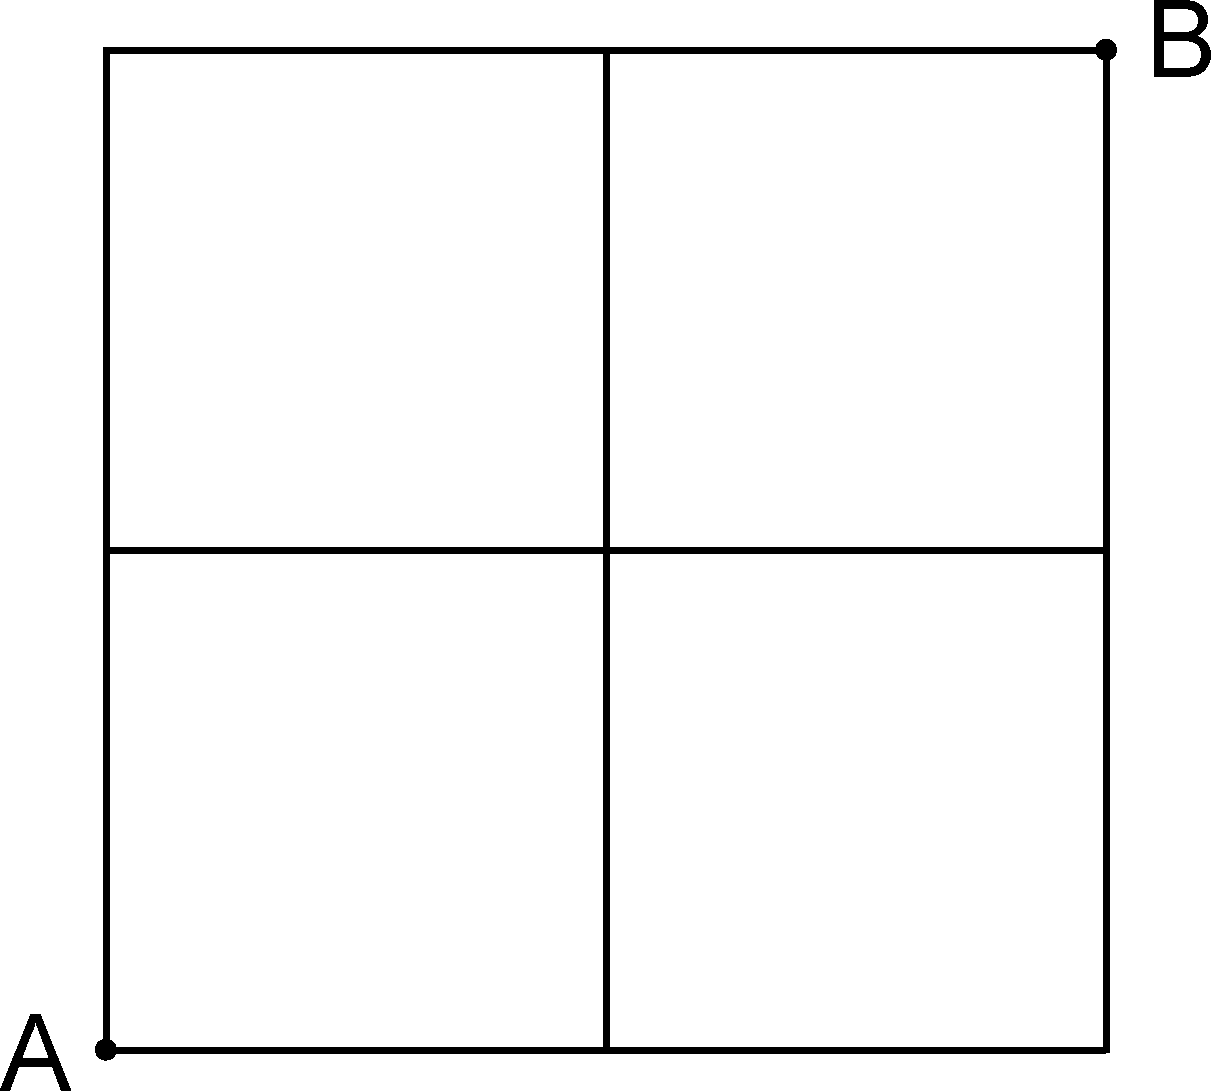
\includegraphics[width=0.2\linewidth]{2014-v3g-01-ruudustik}
\end{center}
\probend
\bigskip

% P56
\setAuthor{Hans Daniel Kaimre}
\setRound{lahtine}
\setYear{2015}
\setNumber{G 2}
\setDifficulty{3}
\setTopic{Elektriahelad}

\prob{Resistors}
\probeng
Find the total resistance $R_{AB}$ of a circuit diagram which consists of identical resistors. The resistance of each resistor is $R$. 
\begin{figure}[h]
\centering
\begin{circuitikz}[scale=0.9] \draw

(0,0) to [resistor] (0,2)
(0,0) to [resistor] (0,-2)
(0,0) to [resistor, *-*] (2,0)
(2,0) to [resistor] (4,0)
(4,0) to [resistor, *-*] (6,0)
(2,0) to [resistor, -*] (2,2)
(2,0) to [resistor, -*] (2,-2)
(4,0) to [resistor, -*] (4,2)
(4,0) to [resistor, -*] (4,-2)
(-1,0) to [short,o-] (0,0)
(6,0) to [short,-o] (7,0)
(0,2) -- (6,2) -- (6,0) -- (6,-2) -- (0,-2)
(-1,0) node[label={above:A}] {}
(7,0) node[label={above:B}] {}
;
\end{circuitikz}
\end{figure}
\probend
\bigskip

% P57
\setAuthor{Kristian Kuppart}
\setRound{lahtine}
\setYear{2016}
\setNumber{G 3}
\setDifficulty{3}
\setTopic{Elektriahelad}

\prob{Circuit diagram}
\probeng
Find the current strength $I$ in the given drawing through the ammeter for two cases: directly after closing the switch and after a long time has passed since closing the switch. Assume that the capacitors are uncharged before closing the switch. The battery is ideal. 
\begin{center}
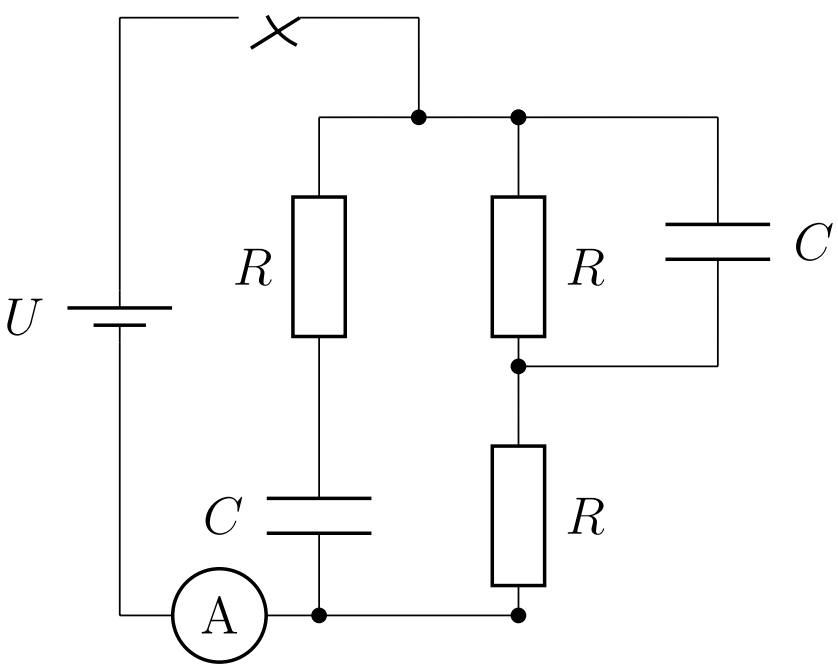
\includegraphics[width=0.45\textwidth]{2016-lahg-03-skeemjoonis}
\end{center}
\probend
\bigskip

% P58
\setAuthor{Kristian Kuppart}
\setRound{lõppvoor}
\setYear{2013}
\setNumber{G 4}
\setDifficulty{4}
\setTopic{Elektriahelad}

\prob{Black box}
\probeng
\begin{wrapfigure}{r}{0.35\textwidth}%
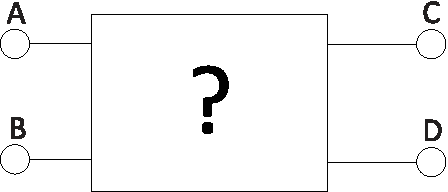
\includegraphics[width=\linewidth]{2013-v3g-04-pilt1}%
\end{wrapfigure}
All the black box’s leads given in the drawing are connected together for a moment. Next, if a battery of voltage $U$ is connected to the leads A and B and a voltmeter is connected with C and D then at the initial moment the voltmeter’s reading is $U$. After the measurement all the leads are connected together again. If the same battery is connected to the leads C and D and the voltmeter to the leads A and B the reading of the voltmeter is $\frac{U}{2}.$ at the initial moment. Knowing that there are only ideal capacitors in the black box, draw the circuit diagram of the black box.
\probend
\bigskip

% P59
\setAuthor{Sandra Schumann}
\setRound{lahtine}
\setYear{2017}
\setNumber{G 4}
\setDifficulty{4}
\setTopic{Elektriahelad}

\prob{Circuit diagram}
\probeng
\begin{wrapfigure}[5]{r}{0.57\textwidth}
	\vspace{-23pt}
	\begin{circuitikz} \draw
		(0.4,0.3) node {A}
		(-0.3,0.6) node {B}
		(-0.3,-0.6) node {C}
		(0,0) node[spdt, xscale=-1] (Sw) {}
		(Sw.out 1) -- (-1.5,0.31)
		(Sw.out 2) -- (-0.59, -1.5) -- (-1.5, -1.5)
		to[american voltage source, l=$9V$] (-1.5,0.31)
		(Sw.in) to[resistor, l=$R$] (3,0) -- (4,0) node[ocirc] {}
		(4.3,0) node {+}
		(4.3,-1.5) node {-}
		(4,-1.5) node[ocirc] {} -- (-0.59, -1.5)
		(3,-1.5) to[capacitor] (3,0)
		;
	\end{circuitikz}
\end{wrapfigure}
A circuit diagram of an electronics device’s part is given in the figure. The diagram consists of a 9 V current source, a filter made of a capacitor and a resistor, a switch and output leads. The two possible positions of the switch are “on” (A and B are connected) and “off” (A and C are connected).\\
If in the given circuit the switch is turned from the position “on” to “off” (that means to turn the device off) and next the voltage source’s polarity is reversed then the electronics device will still work after turning it on. However, if the voltage source’s polarity is changed without turning the device off, then the resistor $R$ will fuse. Assuming that the resistor will fuse when the power on it exceeds 0,25 W, find the minimal and maximal value of $R$.
\probend
\bigskip

% P60
\setAuthor{Jaan Kalda}
\setRound{lõppvoor}
\setYear{2012}
\setNumber{G 3}
\setDifficulty{5}
\setTopic{Elektriahelad}

\prob{Whetstone bridge}
\probeng
In the circuit diagram given in the figure there are identical resistors with resistances $R_1 = R_2 = R_3 = R_4 = R$ and identical batteries with electromotive forces ${\cal E}_1 = {\cal E}_2
= {\cal E}$. Find the current strengths in the resistors (that means the expressions of $I_1$, $I_2$, $I_3$ and $I_4$ through the values of $R$ and ${\cal E}$).
\begin{center}
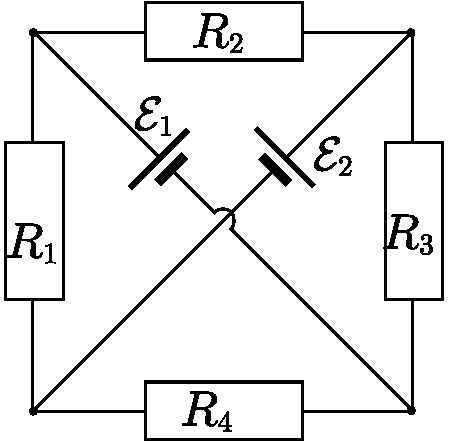
\includegraphics[width=0.35\linewidth]{2012-v3g-03-elektriline_sild}%
\end{center}
\probend
\bigskip

% P61
\setAuthor{Jaan Kalda}
\setRound{lõppvoor}
\setYear{2015}
\setNumber{G 4}
\setDifficulty{5}
\setTopic{Elektriahelad}

\prob{Black box}
\probeng
In a black box there is a circuit diagram made of three resistors and an ideal ammeter. In addition the black box has three output leads $A$, $B$ and $C$. If a voltage $U=\SI{12}{V}$ is applied between the leads $A$ and $B$ then the ammeter’s reading is $I_{AB}=\SI{2}{A}$. In the case of the leads $A$ and $C$ the reading is $I_{AC}=\SI{4}{A}$ and for the leads $B$ and $C$ it is $I_{BC}=\SI{6}{A}$. Draw the circuit diagram in the black box and mark the resistances of the resistors on it.
\probend
\bigskip

% P62
\setAuthor{Jaan Kalda}
\setRound{lõppvoor}
\setYear{2017}
\setNumber{G 6}
\setDifficulty{5}
\setTopic{Elektriahelad}

\prob{Pentagon}
\probeng
Find the readings of the ammeter and the voltmeter in the circuit diagram given in the drawing. All the resistors have a resistance $R=\SI{1}{\ohm}$, voltage on the battery’s leads is $U=\SI{7}{\volt}$. 
\begin{center}
	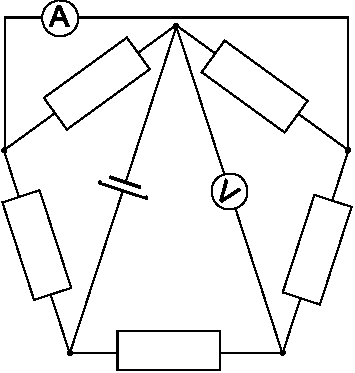
\includegraphics[width=0.4\textwidth]{2017-v3g-06-viisnurk}
\end{center}
\probend
\bigskip

% P63
\setAuthor{Valter Kiisk}
\setRound{piirkonnavoor}
\setYear{2018}
\setNumber{G 8}
\setDifficulty{5}
\setTopic{Elektriahelad}

\prob{12 Lamps}
\probeng
Juku has 12 identical flashlight’s bulbs and a battery. The voltage on the battery’s leads is exactly 5 times bigger than the bulb’s nominal voltage. Juku also found a resistor which has a resistance two times smaller than the resistance of the bulb’s filament in working regimen (the latter was found by dividing the nominal voltage written on the bulb’s socle by the nominal current written on it).\\
\osa How must be the mentioned components connected to a circuit diagram so that all the 12 light bulbs operate with nominal brightness?\\
\osa How many times will the total power of the lights increase (or decrease) if one of the bulbs fuses? Do not account for the relation between the resistance of the lamps and the temperature.
\probend
\bigskip

% P64
\setAuthor{Eero Vaher}
\setRound{piirkonnavoor}
\setYear{2014}
\setNumber{G 8}
\setDifficulty{6}
\setTopic{Elektriahelad}

\prob{Circuit diagram’s energy}
\probeng
Connected in series in a closed circuit diagram is a resistor of resistance $R=\SI{100}{\ohm}$, a capacitor of capacity $C=\SI{200}{\nano\farad}$, inductive coil with a negligible active resistance and with an inductance $L=\SI{10}{\milli\henry}$ and appropriately connected ideal measuring devices. In the moment $t_0$ it was measured that the current strength through the capacitor was $I=\SI{300}{\milli\ampere}$ and that the voltage on the coil was $U=\SI{50}{\volt}$. It is known that at the moment of taking measurements the current in the coil is directed from a region with a higher potential towards a region with a lower potential. Did the capacitor or the inductor have more energy at the moment $t_0$ of taking measurements?
\probend
\bigskip

% P65
\setAuthor{Sandra Schumann}
\setRound{lõppvoor}
\setYear{2016}
\setNumber{G 7}
\setDifficulty{6}
\setTopic{Elektriahelad}

\prob{Current sources}
\probeng
Let us look at the circuit diagram given in the drawing where the circuit element marked as an arrow is a constant current source with a current $I=\SI{2}{mA}$ towards the direction of the arrow. Find the voltage $U$ on the output leads and the current through the resistor $R=\SI{10}{k\ohm}$ for two cases: $\textbf{a)}$ when the switch K is closed and $\textbf{b)}$ when the switch is opened.
\begin{center}
	\begin{circuitikz}[american voltages] \draw
		(0,0) to[battery1, l=$\SI{1}{V}$] (0,1.5)
		to[american current source, l=$\SI{2}{mA}$] (0,3) --(0,4)
		to[european resistor, l=$\SI{10}{k\ohm}$, *-] (2,4)
		to[battery1, l=$\SI{2}{V}$] (4,4)
		to[european resistor, l_=$\SI{5}{k\ohm}$, *-] (4,0) -- (5,0)
		to[battery1, l_=$\SI{3}{V}$] (5,4) -- (4,4)
		(4,0) to[short, *-*] (0,0)
		(0, 1.3) to[short,*-] (1.2, 1.3) -- (1.2, 2.05);\draw[thick] (1.2, 2.05) -- +(60:0.5) ;
		\draw (1.2,2.55) -- (1.2,3.3) to[short,-*] (0,3.3)
		(0,4) to[short, -*] (-2,4)
		to [open, v_<=$U$] (-2,0)
		to[short, *-] (0,0)
		
		(1.5, 2.2) node[right] {K};
	\end{circuitikz}
\end{center}
\probend
\bigskip

% P66
\setAuthor{Eero Vaher}
\setRound{lõppvoor}
\setYear{2018}
\setNumber{G 7}
\setDifficulty{6}
\setTopic{Elektriahelad}

\prob{Finding resistances}
\probeng
\begin{wrapfigure}[10]{r}{0.4\textwidth}
\vspace{-20pt}
\begin{resizebox}{\linewidth}{!}{
\begin{circuitikz}
\draw
(1,0) to[battery1,l_=${U_0=\SI{14}{V},\,I_0=\SI{10}{A}}$] (8,0) to (1,0) to (1,2.5) to (2,2.5) to[short, *-] (2,4) to[resistor,l=${R_1}$, -*] (4.5,4) to[resistor,l=${R_4}$] (7,4) to[short, -*] (7,2.5) to (8,2.5) to (8,0)
(2,2.5) to (2,1) to[resistor,l=${R_2}$, -*] (4.5,1) to[resistor,l=${R_5}$] (7,1) to (7,2.5)
(4.5,1) to[resistor,l_=$R_3$] (4.5,4)
;
\draw[->,thick] (4,2) -- (4,3);
\end{circuitikz}}
\end{resizebox}
\end{wrapfigure}
Five resistors are connected to a current source. Three of them have a resistance of $\SI{1}{\ohm}$, the other two have a same but an unknown resistance. The voltage of the current source is $U_0=\SI{14}{V}$ and its current is $I_0=\SI{10}{A}$. The voltage and the current strength on the third resistor are respectively $U_3=\SI{2}{V}$ and $I_3=\SI{2}{A}$. The direction of the current in the resistor $R_3$ is shown in the drawing. Determine all the resistances of the resistors.
\probend
\bigskip

% P67
\setAuthor{Mihkel Pajusalu}
\setRound{piirkonnavoor}
\setYear{2012}
\setNumber{G 8}
\setDifficulty{7}
\setTopic{Elektriahelad}

\prob{Railway}
\probeng
\begin{wrapfigure}{r}{18mm}%
\vspace{-15pt}
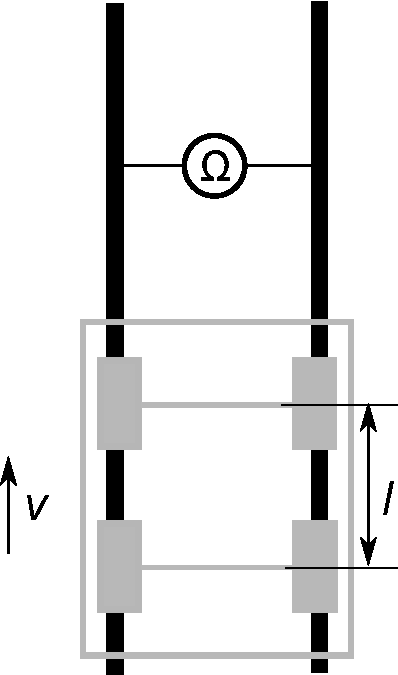
\includegraphics[width=\linewidth]{2012-v2g-08-rong}%
\end{wrapfigure}
Let us measure the electrical resistance between two rails on a railway, like in the drawing. A wagon of speed $v$ drives on the railway. The wagon has two pairs of wheels, one pair is at a distance $l$ from the other. Draw a plot of resistance versus time from the moment when the wagon’s first pair of wheels is at the front of the measuring point at a distance $l/2$ to the moment when the wagon’s rear wheels are behind the measuring point at the distance $l/2$.  Let the resistance of both pairs of the wheels be $r$ and a rail’s resistance per one unit of length $\rho$.
\probend
\bigskip

% P68
\setAuthor{Mihkel Kree}
\setRound{lahtine}
\setYear{2013}
\setNumber{G 9}
\setDifficulty{7}
\setTopic{Elektriahelad}

\prob{Lamps}
\probeng
Juku built a circuit diagram that is shown in the figure using six identical resistors of resistance $R=\SI{10}{\ohm}$, four identical lamps of resistance $r=\SI{20}{\ohm}$ and a voltage source with an electromotive force $\mathcal{E}=\SI{5}{\volt}$. Calculate the power dissipated by each lamp (in the figure marked as 1, 2, 3, 4). Do not account for internal resistance of the voltage source.
\begin{center}
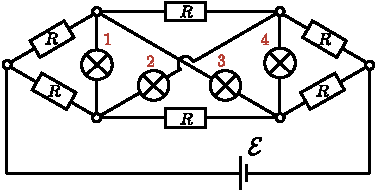
\includegraphics[width=0.6\linewidth]{2013-lahg-09-lambidJoonis-crop}
\end{center}
\probend
\bigskip

% P69
\setAuthor{Jaan Kalda}
\setRound{lahtine}
\setYear{2012}
\setNumber{G 8}
\setDifficulty{8}
\setTopic{Elektriahelad}

\prob{Diodes}
\probeng
\begin{wrapfigure}{r}{0.4\linewidth}
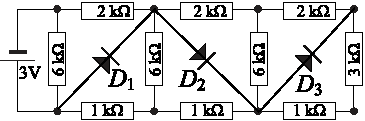
\includegraphics[width=\linewidth]{2012-lahg-08-dioodid}
\end{wrapfigure}
What powers are dissipated by the diodes marked in the figure’s circuit? Assume that the current of the diodes is zero for all the reverse voltages and also for forward voltages below one volt. For a random forward voltage the voltage of the diode is 1,0 V. The values of resistors’ resistances and the electromotive force are marked in the drawing. The direction of a diode’s arrow in the drawing shows the direction of the forward voltage.
\probend
\bigskip

% P70
\setAuthor{Jaan Kalda}
\setRound{lahtine}
\setYear{2016}
\setNumber{G 8}
\setDifficulty{8}
\setTopic{Elektriahelad}

\prob{Octahedron}
\probeng
The drawing shows an octahedron made of wire, the resistances of the wires are written in ohms next to each of them. The wires connecting the ammeters have an insignificantly small resistance. Find the readings of the ammeters.
\begin{center}
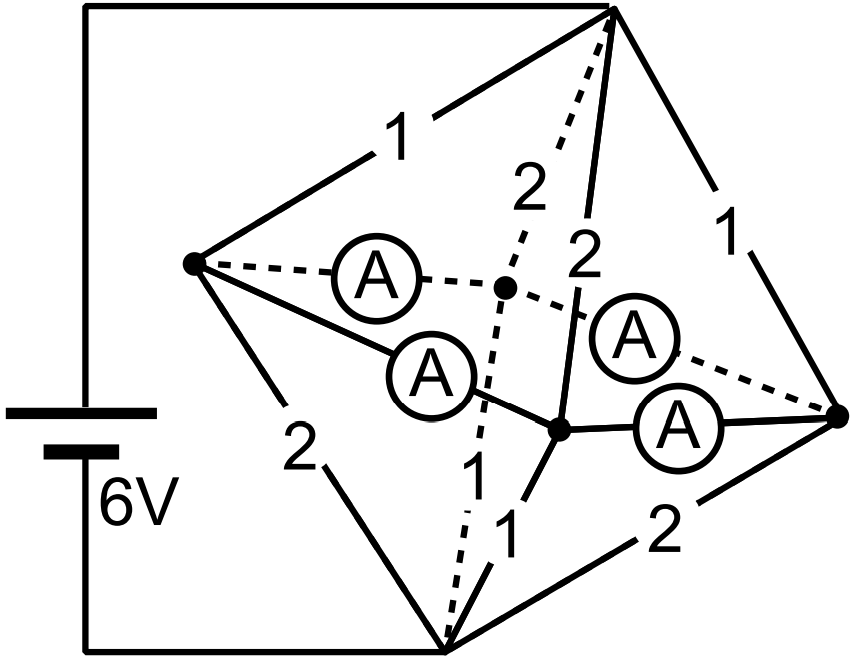
\includegraphics[width=0.5\textwidth]{2016-lahg-08-ampermeeterjoonis}
\end{center}
\probend
\bigskip

% P71
\setAuthor{Jaan Kalda}
\setRound{lõppvoor}
\setYear{2018}
\setNumber{G 9}
\setDifficulty{8}
\setTopic{Elektriahelad}

\prob{Capacitor}
\probeng
\begin{wrapfigure}[7]{r}{0.3\linewidth}
\vspace{-10pt}
\begin{center}
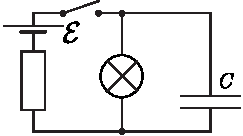
\includegraphics[width=\linewidth]{2018-v3g-09-LC-Q}
\par\end{center} 
\end{wrapfigure}
Let us look at the circuit diagram in the drawing, which is made of a capacitor of capacity $C$, a battery with an electromotive force $\mathcal{E}$, a resistor and an incandescent lamp which can be looked at as a non-linear resistor (the voltage’s dependence on the current is non-linear). At first the capacitor had no charge and the switch was opened. Next, the switch was closed for a short time, after that it was opened again and was held open until the capacitor was completely emptied. During the time when the switch was closed, a heat $Q_1$ was dissipated by the whole circuit; after opening the switch an additional heat $Q_2$ was dissipated. Find the charge that went through the incandescent lamp when the switch was closed.
\probend
\bigskip

% P72
\setAuthor{Jaan Toots}
\setRound{lõppvoor}
\setYear{2015}
\setNumber{G 10}
\setDifficulty{10}
\setTopic{Elektriahelad}

\prob{Thyristor}
\probeng
\begin{wrapfigure}{r}{0.48\textwidth}
\begin{circuitikz} \draw

(0,2) to[resistor=$R$] (2,2)
      to[Do,l=$T_1$, *-*] (2,0) -- (0,0)
      to[battery1,l=$U$] (0,2)
(2,2) to[switch] (4,2)
      to[Do,l=$T_2$] (4,0) -- (2,0)
;
\end{circuitikz}
\end{wrapfigure}
Thyristor’s (an element similar to a diode) V-I curve is shown in the graph. Two such thyristors are connected to a voltage source and a resistor, as in the drawing. The resistance of the resistor is $R = \SI{2}{\kilo\ohm}$.\\
a) At first the switch was opened. The voltage source’s voltage is increased linearly during a time period $t=\SI{42}{\second}$ from the value $U_0=\SI{0}{\volt}$ to the value $U_a = \SI{42}{\volt}$. Sketch the current strength of this circuit as a function of time $I(t)$. What is the current’s final value $I_a$?\\
b) Find the final current strengths in each thyristor if the switch was closed without changing the voltage $U_a$ applied on the circuit. 
\begin{figure}[h]
\begin{center}
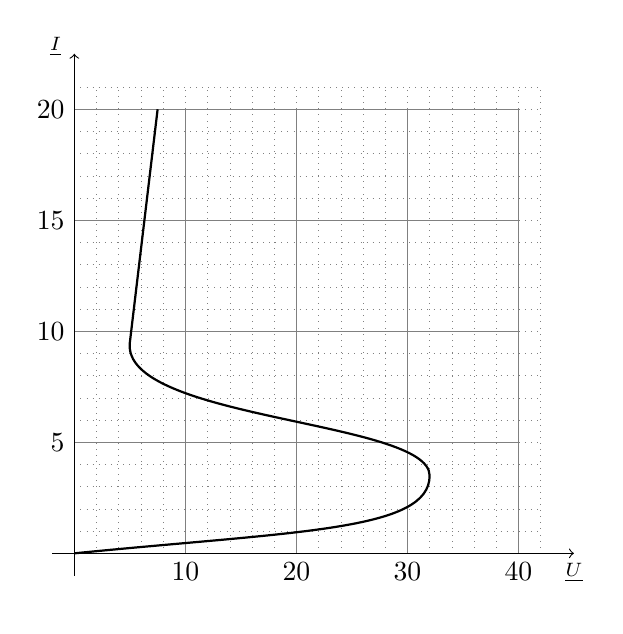
\begin{tikzpicture}[scale=1.41,
axes/.style=]

\draw[step=0.2, gray, dotted, very thin] (0,0) grid (4.2,4.2);
\draw[step=1, gray, very thin] (0,0) grid (4,4);

\begin{scope}[axes]
    \draw[->] (-0.2,0) -- (4.5,0) node[right, below] {$\frac{U}{\si{\volt}}$} coordinate(x axis);
    \draw[->] (0,-0.2) -- (0,4.5) node[above, left] {$\frac{I}{\si{\milli\ampere}}$} coordinate(y axis);

    \foreach \x/\xtext in {1/10, 2/20, 3/30, 4/40}
    \draw (\x,0) node[below] {$\xtext$};
    
    \foreach \y/\ytext in {1/5, 2/10, 3/15, 4/20}
    \draw (0,\y) node[left] {$\ytext$};
\end{scope}

\draw[thick] (0,0) .. controls (2,0.2) and (3.2,0.2) .. (3.2,0.7) .. controls (3.2,1.2) and (5/12,1.2) .. (0.5,1.9) -- (0.75,4);

\end{tikzpicture}

\end{center}
\end{figure}
\probend
\bigskip
\newpage\subsection{\protect\StrSubstitute{Electrostatics}{-}{ }}

% P73
\setAuthor{Madis Ollikainen}
\setRound{lahtine}
\setYear{2012}
\setNumber{G 3}
\setDifficulty{2}
\setTopic{Elektrostaatika}

\prob{Capacitor}
\probeng
Searching through old experimental equipment a physics student found a parallel plate capacitor. Being a young physicist he immediately had the strong wish to test it out. He measured the distance between the capacitor’s plates to be $d$ and next he charged the capacitor to the voltage $U$. Now the student placed a ball between the capacitor’s plates. The ball dropped down on to the bottom plate and then started to rise up again. The time it took the ball to rise from the bottom plate to the upper one was $t$. Find the ratio of the ball’s mass and the charge received from the bottom plate.
\probend
\bigskip

% P74
\setAuthor{Mihkel Kree}
\setRound{lahtine}
\setYear{2017}
\setNumber{G 3}
\setDifficulty{4}
\setTopic{Elektrostaatika}

\prob{Electron}
\probeng
\begin{wrapfigure}[7]{r}{0.5\linewidth}
	\vspace{-10pt}
	\hspace{-10pt}
	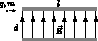
\includegraphics[width=\linewidth]{2017-lahg-03-elJoonisMK}
\end{wrapfigure}
An electron is moving in vacuum and enters a region of space between parallel plates from the area’s upper edge so that the electron’s velocity is parallel to the plates (see figure). How big is the electron’s minimal possible speed $v_\mathrm{min}$ when exiting the area of space between the plates? The length of the plates is $l$ and the distance between them is $d$. Between the plates there is a homogeneous electric field $\vec{E}$, neglect edge effects. The electron’s charge is $q$ and its mass is $m$. Neglect the gravitational force.
\probend
\bigskip

% P75
\setAuthor{Mihkel Kree}
\setRound{piirkonnavoor}
\setYear{2017}
\setNumber{G 9}
\setDifficulty{6}
\setTopic{Elektrostaatika}

\prob{Charges}
\probeng
\begin{wrapfigure}{r}{0.3\textwidth}
	\vspace{-25pt}
	\begin{center}
		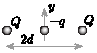
\includegraphics[width=0.32\textwidth]{2017-v2g-09-laengudjoonis}
	\end{center}
	\vspace{-10pt}
\end{wrapfigure}
Two balls, each with a charge $Q$, are firmly fixed so that the distance between their centers is $2d$. A third ball with a charge $-q$ and mass $m$ is placed exactly in the middle of the two balls. The third ball can only move along the $y$-axis (see figure). Find the period $T$ of the third ball’s small oscillations along the $y$-axis.
\probend
\bigskip

% P76
\setAuthor{Jonatan Kalmus}
\setRound{lõppvoor}
\setYear{2018}
\setNumber{G 6}
\setDifficulty{7}
\setTopic{Elektrostaatika}

\prob{Pendulum}
\probeng
An electrically insulated metal ball of mass $M$ and charge $Q>0$ is hanging at the end of a vertical spring of stiffness $k$ in a gravitational field $g$, the ball is in its equilibrium position. Now a vertical electrical field of strength $E$ is created. At the first moment it is directed downwards and afterwards always at the same direction as the ball’s velocity. Assume that the electrical field changes instantaneously. Find the ball’s distance from its initial position at a moment of time $t=7\pi \sqrt{\frac{M}{k}}$.
\probend
\bigskip

% P77
\setAuthor{Stanislav Zavjalov}
\setRound{piirkonnavoor}
\setYear{2012}
\setNumber{G 10}
\setDifficulty{8}
\setTopic{Elektrostaatika}

\prob{Cone}
\probeng
A homogeneously charged cone of height $H$ creates a potential $\varphi_0$ at the cone’s tip $S$. The cone’s tip of height $h$ is cut off and the removed part is displaced to infinity. What is the new potential at the point $S$?
\probend
\bigskip

% P78
\setAuthor{Jaan Kalda}
\setRound{lõppvoor}
\setYear{2012}
\setNumber{G 9}
\setDifficulty{8}
\setTopic{Elektrostaatika}

\prob{Charges}
\probeng
\begin{wrapfigure}{r}{0.33\textwidth}%
\vspace{-10pt}
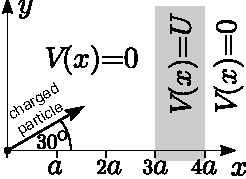
\includegraphics[width=\linewidth]{2012-v3g-09-laeng_ing}%
\end{wrapfigure}
A positively charged particle is accelerated from the origin with the help of a voltage $4U$ (where $U>0$) to a certain velocity which lies on the $x-y$ plane under the angle of $30$ degrees with respect to the $x$-axis (see figure). The electric potential $V(x,y)\equiv V(x)$ only depends on the $x$-coordinate: if $3a<x<4a$ then $V(x)=U$ and if not then $V(x)=0$; besides the electrostatic force no other forces are applied to the particle and $a>0$.\\
\osa Sketch the trajectory of the charge on the $x-y$ plane (you do not have to show the geometrical measurements or angles).\\
\osa The source of the charged particles is now a coaxial vacuum diode at the origin. Because of that the particles accelerated with the voltage $4U$ are moving isotropically (at equal quantities) to all directions of the $x-y$ plane; the $z$-directional component of the velocity for all particles is 0. What part of all the emitted particles reaches the region of space $x>4a$?
\probend
\bigskip

% P79
\setAuthor{Stanislav Zavjalov}
\setRound{lõppvoor}
\setYear{2013}
\setNumber{G 10}
\setDifficulty{8}
\setTopic{Elektrostaatika}

\prob{Capacitor}
\probeng
The area of a capacitor’s square-shaped plates is $S$ and the distance between the plates is $d \ll \sqrt{S}$. The capacitor is charged up to a voltage $U_0$ and after that it is disconnected from the battery. A square-shaped conductive plate is placed in to the capacitor, also with the area $S$ and with a width $d/2$, until the plate is completely in the capacitor. During this process the plate does not touch the capacitor’s plates and is parallel to them. How much work was done by bringing the plate in? Explain if the plate pulled itself in or did external forces have to push it in. Neglect edge effects. Vacuum’s relative permittivity is $\varepsilon_0$.
\probend
\bigskip

% P80
\setAuthor{Jaan Kalda}
\setRound{lahtine}
\setYear{2017}
\setNumber{G 7}
\setDifficulty{8}
\setTopic{Elektrostaatika}

\prob{Capacitor}
\probeng
\begin{wrapfigure}[5]{r}{0.35\linewidth}
	\vspace{-13pt}
	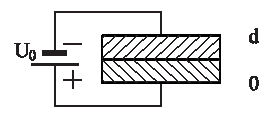
\includegraphics[width=\linewidth]{2017-lahg-07-res-cap2}
\end{wrapfigure}
The distance between the plates of a parallel plate capacitor is $d$. The capacitor’s capacity is $C$. Two dielectric plates of width $d/2$ are placed between the capacitor’s plates. The relative permittivity of one plate is $\varepsilon$, the other’s is $2\varepsilon$. What is the capacity of the capacitor now? What is the charge at the interface between the two plates if a voltage $U_0$ is applied to the capacitor?
\probend
\bigskip

% P81
\setAuthor{Jaan Kalda}
\setRound{piirkonnavoor}
\setYear{2015}
\setNumber{G 10}
\setDifficulty{9}
\setTopic{Elektrostaatika}

\prob{Chargeless rod}
\probeng
a) A dielectric rod of mass $m$ and length $L$ carries a positive charge $q$ on each of its tips (the middle of the rod is chargeless, therefore the total charge is $2q$). In the region $x<0$ there is a $x$-directional electric field with a strength $E_0$ and in the region $x>0$ there is an electric field with the same strength, but it is antiparallel to the $x$-axis. The center of the rod is at the origin and the rod is parallel to the $x$-axis. The rod is given an initial speed $v$ directed towards the $x$-axis. Find the period of the oscillations. The rod is placed so that it cannot rotate, it can only move along the $x$-axis.\\
b) Find the period of the small oscillations when the configuration stays the same, only that instead of the point charges there is a total charge $Q$ evenly distributed all over the rod.
\probend
\bigskip

% P82
\setAuthor{Jaan Kalda}
\setRound{lahtine}
\setYear{2016}
\setNumber{G 10}
\setDifficulty{9}
\setTopic{Elektrostaatika}

\prob{Balls}
\probeng
Two metal balls of radius $R$ are connected to each other with a thin metal wire. The balls are in a homogeneous electric field of strength $E$. The length of the metal wire is $l$, furthermore $l\gg R$. The system is at equilibrium. Find the mechanical tension $T$ in the wire.
\probend
\bigskip

% P83
\setAuthor{Jaan Kalda}
\setRound{lõppvoor}
\setYear{2018}
\setNumber{G 10}
\setDifficulty{9}
\setTopic{Elektrostaatika}

\prob{Two balls}
\probeng
Two identical metal balls of radius $R$ and mass $m$ are connected to each other with a thin steel wire of length $L\gg R$. In the region $x\ge 0$ there is an electric field of strength $E$ and it is directed along the $x$-axis. In the region $x< 0$ there is no electric field. At the initial moment the balls are still and are at the distance $L$ from each other so that the wire is taut and parallel to the $x$-axis. The center of one ball is at a point $x=R$, the other ball is in the region $x<0$. Qualitatively sketch a graph depicting the dependence of the balls’ speed on time (a quantitative time scale is not needed) and find their speed while passing through the point $x=2L$. The capacity of the steel wire is negligibly small.
\probend
\bigskip

% P84
\setAuthor{Jaan Kalda}
\setRound{lõppvoor}
\setYear{2016}
\setNumber{G 10}
\setDifficulty{10}
\setTopic{Elektrostaatika}

\prob{Three balls}
\probeng
Three little balls of mass $m$ are carrying the same electric charge $q$ and are connected with threads made of insulation material so that they form a triangle $ABC$, where $\angle BAC=120^\circ$ and the length of the thread $|BC|=L$ opposite to the ball $A$. The thread $BC$ is cut broken. Find a) the ball $A$’s maximal speed during subsequent motion and b) the accelerations of the balls momentarily after cutting through the thread. Neglect gravitational interaction.
\probend
\bigskip
\newpage\subsection{\protect\StrSubstitute{Gases}{-}{ }}

% P85
\setAuthor{Eero Vaher}
\setRound{lõppvoor}
\setYear{2015}
\setNumber{G 1}
\setDifficulty{2}
\setTopic{Gaasid}

\prob{balloon}
\probeng
A balloon filled with helium can lift a weight with a mass up to $M=\SI{200}{kg}$. What is the volume of the balloon $V$? The volume of the weight is negligible. The mass of the balloon’s shell is included in the mass of the weight. The air density is $\rho=\SI{1.2}{kg\per m^3}$, air pressure $p=\SI{100}{kPa}$, air temperature $T=\SI{20}{\degreeCelsius}$. The molar mass of helium is $\mu=\SI{4.0}{g\per mol}$, universal gas constant is $R=\SI{8.3}{J\cdot mol^{-1}\cdot K^{-1}}$.
\probend
\bigskip

% P86
\setAuthor{Eero Vaher}
\setRound{lahtine}
\setYear{2013}
\setNumber{G 4}
\setDifficulty{3}
\setTopic{Gaasid}

\prob{The might of balloon}
\probeng
A balloon filled with helium can lift a weight with a mass up to 100 kg on Earth. What is the mass of the weight that an identical balloon can lift on Mars (the mass of the balloon is included in the mass of the weight)? The volume of the weight is negligible. The air density on Earth is $\rho_0=\SI{1.2}{\kilogram\per\meter^3}$, air pressure on Earth $p_0=\SI{100}{\kilo\pascal}$, air temperature on $T_0=\SI{20}{\degreeCelsius}$, “air” density on Mars is $\rho_1=\SI{0.015}{\kilogram\per\meter^3}$, “air” pressure on Mars $p_1=\SI{600}{\pascal}$, “air” temperature on Mars $T_1=\SI{-60}{\degreeCelsius}$. The molar mass of helium is $\mu=\SI{4.0}{\gram\per\mole}$, universal gas constant is $R=\SI{8.3}{\joule\per\kelvin\per\mole}$.
\probend
\bigskip

% P87
\setAuthor{Mihkel Kree}
\setRound{lõppvoor}
\setYear{2014}
\setNumber{G 3}
\setDifficulty{4}
\setTopic{Gaasid}

\prob{Expansion vessel}
\probeng
A house’s heating system consists of a big accumulator vessel, in which circulating hot water is kept and an expansion vessel to compensate water’s thermal expansion. The expansion vessel is a vessel with a fixed volume, one part of the vessel is filled with air, the rest is filled with water originating from the heating system that can freely flow back into the system. When all of the water reached the room temperature $t_0=\SI{20}{\degreeCelsius}$, the expansion vessel was filled with compressed air so that the air volume in the vessel was $V_1=\SI{0.080}{m^3}$ and pressure $p_1=\SI{1.5}{}\,p_0$, where $p_0=\SI{0.10}{\mega\pascal}$ is atmosphere pressure. At room temperature the volume of the water in the whole system is $V_0=\SI{1.0}{m^3}$.\\
There is also an emergency valve in the piping to avoid the bursting of the pipes. The valve opens when the pressure in the piping exceeds atmosphere pressure by $\Delta p = \SI{1.2}{} \, p_0 $. To what temperature can the water in the system be heated without there being an accident? Neglect metal’s thermal expansion. The ratio between the density of water and temperature is shown in the graph. Assume that the graph’s shape does not depend on the pressure (the changes in pressures are too small for that). Also assume that the air temperature in the expansion vessel stays at room temperature $t_0$.
\begin{center}
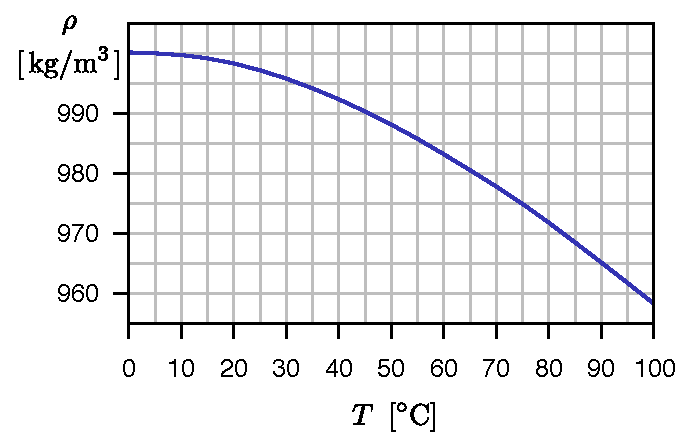
\includegraphics[width=0.8\linewidth]{2014-v3g-03-veeTihedus}
\end{center}
\probend
\bigskip

% P88
\setAuthor{Kaur Aare Saar}
\setRound{lahtine}
\setYear{2015}
\setNumber{G 3}
\setDifficulty{4}
\setTopic{Gaasid}

\prob{Gas tank}
\probeng
A tall cylindrical compressed gas tank of radius $r=\SI{0,3}{m}$ is made of steel that tolerates force per unit of area up to $\sigma=\SI{250}{MPa}$. Find the largest pressure of gas in the gas tank that the tank can endure. The width of the tank’s wall is $t=\SI{2}{mm}$.
\probend
\bigskip

% P89
\setAuthor{Mihkel Kree}
\setRound{piirkonnavoor}
\setYear{2016}
\setNumber{G 5}
\setDifficulty{4}
\setTopic{Gaasid}

\prob{Sauna’s door}
\probeng
The air temperature in a sauna’s steam room of volume $V=\SI{10}{m^3}$ is $t=\SI{90}{\degreeCelsius}$. Water with a mass $m=\SI{150}{g}$ is cast on the stove for steam and it vaporizes immediately. Let us think hypothetically that the steam room is hermetically closed. With what force should the sauna visitors hold the handle of a door of area $A=\SI{2,0}{m^2}$ so that the door would open? The gas constant is $R=\SI{8.3}{J \per (mol\!\cdot\! K)}$ and the molar mass of water is $\mu=\SI{18}{g\per mol}$. If you solve the problem correctly you will probably discover that the force found is unusually large. Explain with a sentence why in reality the force needed to open the door in a sauna is not that big.
\probend
\bigskip

% P90
\setAuthor{Ardi Loot}
\setRound{lahtine}
\setYear{2017}
\setNumber{G 5}
\setDifficulty{4}
\setTopic{Gaasid}

\prob{Bicycle hike}
\probeng
\begin{wrapfigure}[6]{r}{0.4\linewidth}
	\vspace{-15pt}
	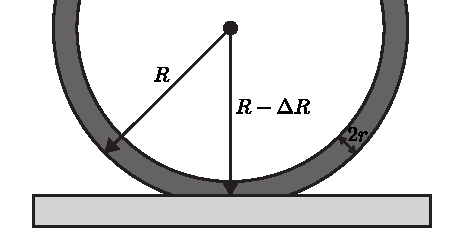
\includegraphics[width=5cm]{2017-lahg-05-fig_rattakumm}
\end{wrapfigure}
Juku is on a bicycle hike and wants to pump a little more air into his bike’s rear wheel. To make things easier, Juku packs his heavy hike equipment off the rack and turns the bike upside down (wheels are directed towards the sky). Estimate by how many percent smaller force he needs to apply while pumping as compared to the situation where the equipment was still on. The radius of the wheel is $R=\SI{33.0}{cm}$, radius of the tire $r=\SI{2.5}{cm}$, the mass resting on the rear wheel (the wheel together with the hike equipment) $m=\SI{30}{kg}$, the gauge pressure in the wheel under the load $p=\SI{150}{kPa}$, air pressure $p_{0}=\SI{100}{kPa}$ and gravitational acceleration $g=\SI{9.8}{m/s^{2}}$.\\
\emph{Hint.} The mass of the wheel without the load is given by an equation $V=2\pi^{2}\left(R-r\right)r^{2}$ and with loading it decreases by $\Delta V\approx S\cdot\Delta R/2$, where $S\approx2\pi\Delta R\sqrt{Rr}$ is the area of contact between the tire and the ground and $\Delta R\ll r$ is the range of tire’s deformation (see figure).
\probend
\bigskip

% P91
\setAuthor{Rasmus Kisel}
\setRound{piirkonnavoor}
\setYear{2017}
\setNumber{G 6}
\setDifficulty{4}
\setTopic{Gaasid}

\prob{Cylinder in refrigerator}
\probeng
In a closed cylinder of inner radius $R$ and inner height $h$ there is a liquid that fills a fraction $k$ of the cylinder's inner volume. Initially the cylinder is at room temperature $T_{1}$. The cylinder is put into a freezer with a constant temperature $T_{2}$, which is below the melting temperature of the substance in the cylinder. It is known that the density of the substance in liquid form is $\rho_0$ and in solid form $\lambda\rho_0$. Find how many times the air pressure in the cylinder changes after the liquid has been frozen compared with the initial state. Assume that the cylinder's dimension do not change due to the liquid’s freezing.
\probend
\bigskip

% P92
\setAuthor{Tundmatu autor}
\setRound{lahtine}
\setYear{2011}
\setNumber{G 5}
\setDifficulty{5}
\setTopic{Gaasid}


\bigskip

% P93
\setAuthor{Andreas Valdmann}
\setRound{piirkonnavoor}
\setYear{2012}
\setNumber{G 6}
\setDifficulty{5}
\setTopic{Gaasid}

\prob{hot air balloon}
\probeng
To what temperature should the air in a hot air balloon be heated so that the balloon would fly up? The outside air temperature is $t=\SI{20}{\degreeCelsius}$, the balloon's volume is $V=\SI{3000}{m^3}$ and it does not change. The total mass of the balloon's shell and load is $m=\SI{700}{kg}$ and the air density at 20 degrees is $\rho_{20}=\SI{1,2}{kg/m^3}$.
\probend
\bigskip

% P94
\setAuthor{Andreas Valdmann}
\setRound{lõppvoor}
\setYear{2012}
\setNumber{G 4}
\setDifficulty{5}
\setTopic{Gaasid}

\prob{Basketball}
\probeng
The mass of a basketball meeting the standards of NBA is $m=\SI{600}{g}$, circumference $C=\SI{76}{cm}$ and gauge pressure in the ball $p_1=\SI{55}{kPa}$. How deep should the basketball be pushed into water so that it would start to sink down by itself? The density of water is $\rho=\SI{1000}{kg/m^3}$, gravitational acceleration $g=\SI{9,8}{m/s^2}$ and the air pressure on the water's surface is $p_0=\SI{100}{kPa}$. You can assume that during the sinking the air temperature in the ball does not change and that the mass of the ball’s shell is negligible.
\probend
\bigskip

% P95
\setAuthor{Ardi Loot}
\setRound{lahtine}
\setYear{2016}
\setNumber{G 7}
\setDifficulty{6}
\setTopic{Gaasid}

\prob{Expansion vessel}
\probeng
An expansion vessel is added to a heating system to avoid the overpressure forming in the system due to the expansion of water. The vessel consists of a cylinder of volume $V,$ that is divided into two parts by a freely moving thin partition. One of these parts is filled with compressed air ($T_{0}=\SI{20}{\degreeCelsius}$) to a pressure $p_{0}$, taking under it all of the cylinder’s volume. Next, the other part of the cylinder is connected to the heating system at a temperature $T_{1}=T_{0}$ and the system is filled with water until a pressure $p_{1}=\SI{300}{kPa}$ is reached and the total volume of the water in the system is $V_{s}=\SI{100}{L}$. After this $\beta=10\%$ of the expansion vessel is filled with water. In winter the volume of the water in the system increases by $\alpha=\SI{1}{\%}$ due to the heating and in result the pressure of the system increases to $p_{2}$, moreover the air in the expansion vessel is warmed to a temperature $T_{2}=\SI{40}{\degreeCelsius}$. Find how big must be the initial air pressure $p_{0}$ in the expansion vessel and the minimal volume of the vessel $V$, so that the extra pressure $\Delta p=p_{2}-p_{1}$ formed in result of the water’s expansion would not be bigger than 50 kPa.
\probend
\bigskip

% P96
\setAuthor{Valter Kiisk}
\setRound{piirkonnavoor}
\setYear{2017}
\setNumber{G 8}
\setDifficulty{7}
\setTopic{Gaasid}

\prob{Steel vessel}
\probeng
The inner diameter of a spherical steel vessel is $d=\SI{0.5}{m}$ and the mass $m=\SI{25}{kg}$. Maximally how many liters of gas (corresponding to normal pressure) would it be possible to store in that vessel at high pressure? The density of steel is $\rho=\SI{7.9}{g/cm^3}$ and the maximal tolerable pulling force per unit of area $\sigma=\SI{450}{MN/m^2}$. Normal pressure is $p_0=\SI{101.3}{kPa}$.
\probend
\bigskip

% P97
\setAuthor{Ardi Loot}
\setRound{lõppvoor}
\setYear{2017}
\setNumber{G 7}
\setDifficulty{7}
\setTopic{Gaasid}

\prob{Balloon}
\probeng
Juku wants to pump a balloon full. He has a big pump which has an initially closed valve at the end. He attaches the balloon to the end of the pump, then presses onto the pump until the pressure in the pump rises to $p$. As a result of this pressure the air temperature in the pump rises to $T$. Juku turns the valve open and the balloon starts to fill slowly. At the same time the handle of the pump slowly sinks down. During the whole process Juku presses onto the pump with the exact same force as in the beginning. What is the air temperature in the balloon if it is pumped completely full? Do not take the heat losses through the pump and the balloon’s walls into account, as well as the work done during the stretching of the balloon’s rubber. The outer air pressure and temperature is $p_0$ and $T_0$. The heat capacity of air at constant volume is $c_V$.
\probend
\bigskip

% P98
\setAuthor{Ants Remm}
\setRound{piirkonnavoor}
\setYear{2014}
\setNumber{G 10}
\setDifficulty{8}
\setTopic{Gaasid}

\prob{hot air balloon}
\probeng
Juku goes flying with a spherical hot air balloon of radius $r = \SI{8.7}{\metre}$. The mass together with the passengers is $M_0= \SI{390}{\kg}$ and in addition $M_k = \SI{20}{\kg}$ of propane is brought along for fuel. How long can Juku's balloon flight last?\\ 
The balloon is covered with a cover that decreases thermal conductivity and thermal radiation to negligible values. In working state the air permeates through the balloon's shell with a speed $\lambda = \SI{500}{g\per\s}$. The air pressure and temperature in the flight's height is $p_0 = \SI{100}{\kilo\Pa}$ and $T_0 = \SI{10}{\degreeCelsius}$. Propane's calorific value is $k = \SI{50}{MJ/kg}$. Air's average molar mass is $\mu = \SI{29}{g\per\mole}$ and the heat capacity at constant pressure $C_p = \SI{1.0}{\frac{kJ}{K\cdot kg}}$. Universal gas constant is $R = \SI{8.3}{\frac{J}{K\cdot mol}}$.
\probend
\bigskip

% P99
\setAuthor{Jaan Kalda}
\setRound{lõppvoor}
\setYear{2018}
\setNumber{G 8}
\setDifficulty{8}
\setTopic{Gaasid}

\prob{Rising balloon}
\probeng
During a beautiful sunny weather the atmosphere is usually adiabatic. It means that the air masses are in a continuous up and down movement. When rising the air expands and cools adiabatically; because of the continuous mixing the temperature of the rising air mass is equal to the temperatures of the air masses surrounding it at the given height. It is possible to show that during this case the temperature decreases linearly with the height, $T=T_0-\frac{\gamma-1}\gamma\frac{\mu g h}R$, where $\gamma=\SI{1.4}{	}$ is air's adiabatic index, $\mu=\SI{29}{g/mol}$ — air's average molar mass, $g=\SI{9.81}{m/s^2}$ — gravitational acceleration, $R=\SI{8.31}{J/mol.K}$ —universal gas constant and $h$ — height from the ground, the air temperature on the ground $T_0=\SI{293}K$. The balloon is made of non-stretchable but freely flexible leather that can maximally contain $V_0$ amount of gas; the amount of helium that the balloon is filled with occupies a volume $V_0/2$ on the ground. The balloon is let free and it starts to slowly rise; assume that the temperature of the helium in the balloon is always equal to the temperature of the surrounding air. Evaluate at what height $h_1$ is the balloon's buoyancy force $1\%$ less than on the ground. The evaluation's relative error is expected to be less than one tenth, moreover there is no need to prove that the error is sufficiently small.\\
\emph{Note.}  During an adiabatic process the relation $pV^\gamma = \const$ applies, where $p$ is the pressure of the gas and $V$ the volume.
\probend
\bigskip
\newpage\subsection{\protect\StrSubstitute{Geometrical optics}{-}{ }}

% P100
\setAuthor{Roland Matt}
\setRound{lahtine}
\setYear{2011}
\setNumber{G 1}
\setDifficulty{2}
\setTopic{Geomeetriline optika}

\prob{Disorder in an optics laboratory}
\probeng
An optician was cleaning an old laboratory and found an unmarked concave lens and a convex lens. To determine their optical powers he positioned the lenses in a straight line and directed two parallel laser rays through them, the distance between the rays was $x_{1}=\SI{1,0}{cm}$. He changed the distance between the lenses until the rays leaving the system were also parallel (he controlled that by determining the distance between them with a sheet of paper at different lengths), now the distance between the rays was $x_{2}=\SI{26}{mm}$. In that situation the distance between the lenses was $d=\SI{32}{cm}$. What was the optical power of the lenses?
\probend
\bigskip

% P101
\setAuthor{Koit Timpmann}
\setRound{piirkonnavoor}
\setYear{2016}
\setNumber{G 3}
\setDifficulty{2}
\setTopic{Geomeetriline optika}

\prob{Lens}
\probeng
Point $A$ and its real image $A'$ are respectively at the distances 4 cm and 1 cm from the optical axis of the lens. The distance between the point $A$ and its image $A'$ is 15 cm. How big is the focal length of the lens?
\probend
\bigskip

% P102
\setAuthor{EFO žürii}
\setRound{lahtine}
\setYear{2017}
\setNumber{G 2}
\setDifficulty{2}
\setTopic{Geomeetriline optika}

\prob{The image of a light source}
\probeng
A concave lens and a convex lens have the same focal length with an absolute value $f$. The lenses are positioned so that their focuses and optical axes coincide. In front of the lenses on the optical axis there is a point light source $A$ at a distance $1,5f$ from the convex lens. Find the location of the point light source's image formed by the two-lens system. Make a draft.
\probend
\bigskip

% P103
\setAuthor{Aigar Vaigu}
\setRound{piirkonnavoor}
\setYear{2017}
\setNumber{G 4}
\setDifficulty{2}
\setTopic{Geomeetriline optika}

\prob{Ethanol factory}
\probeng
In an ethanol factory, with the help of the optical device shown in the figure, the volume percentage of ethanol is measured in a spirit and water mixture. The mixture is located in a canal of width $d=\SI{1}{cm}$. By what distance does the location of the ray on the device's photosensitive element change if the ethanol with a volume percentage 40 \% is replaced by an ethanol with a volume percentage 85 \%? You can assume that the refractive index $n\idx{mix}$ of the mixture is a linear combination of the refractive indexes of water and spirit
$$
n\idx{mix}=Xn\idx{ethanol}+(1-X)n\idx{water},
$$
where X is ethanol’s volume content ranging from 0 to 1, $n\idx{ethanol}=\num{1,3615}$ and $n\idx{water}=\num{1,3330}$.
\begin{center}
	\vspace{-0pt}
	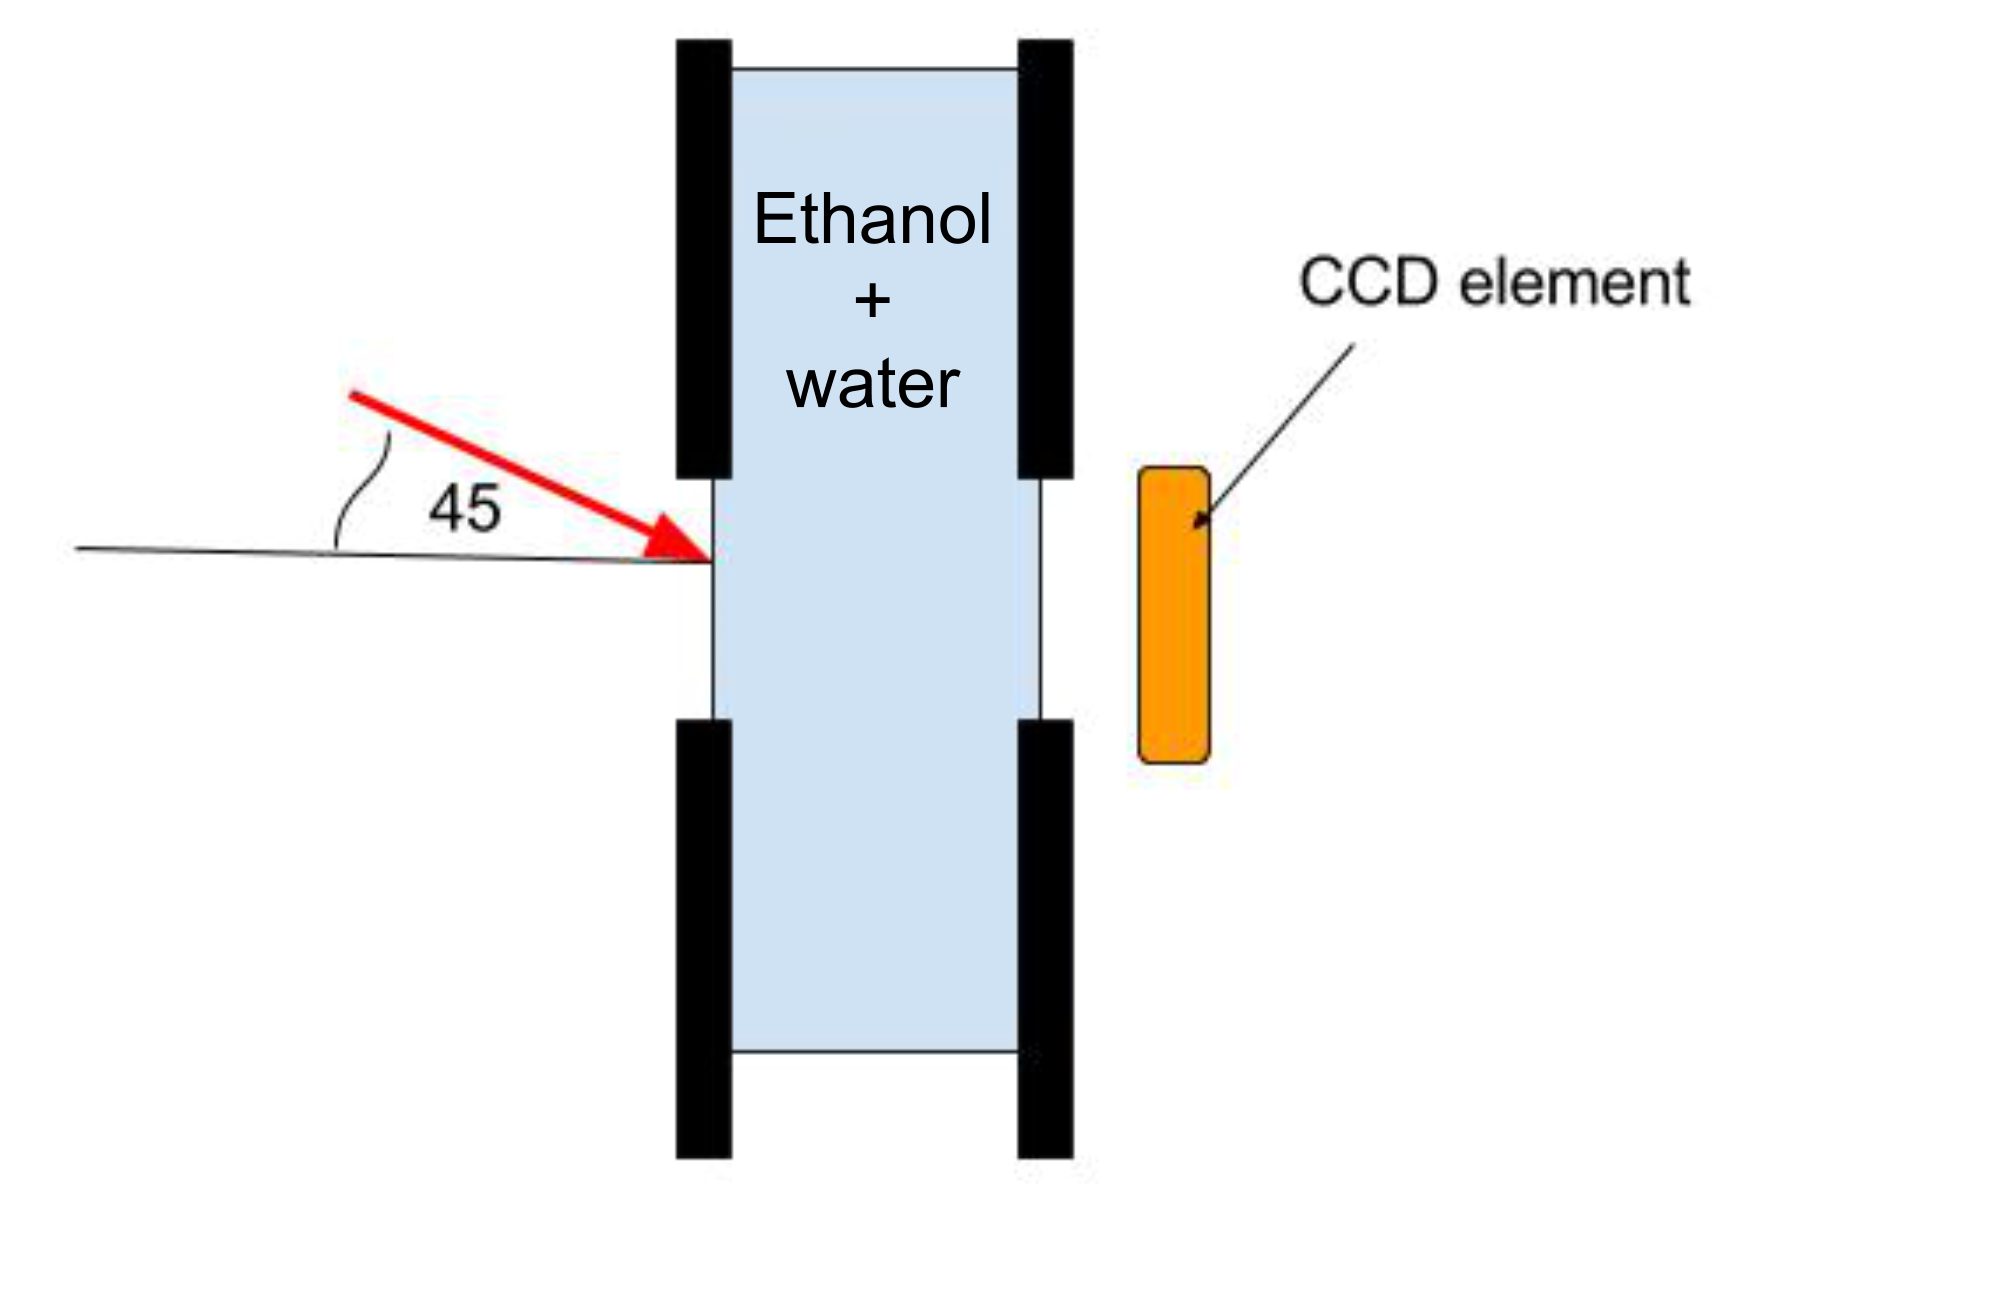
\includegraphics[width=0.5\linewidth]{2017-v2g-04-Piiritusetehas_ing}
	\vspace{-10pt}
\end{center}
\probend
\bigskip

% P104
\setAuthor{EFO žürii}
\setRound{piirkonnavoor}
\setYear{2018}
\setNumber{G 2}
\setDifficulty{2}
\setTopic{Geomeetriline optika}

\prob{Two light sources}
\probeng
Two point light sources are positioned on different points of a convex lens’ optical axis. The images of these light sources formed by the lens coincide. It is known that one light source is at a distance $a=\SI{18}{cm}$ from the center of the lens. How far is the other light source distanced from this light source? The focal length of the lens is $f=\SI{9}{cm}$.
\probend
\bigskip

% P105
\setAuthor{Hans Daniel Kaimre}
\setRound{lõppvoor}
\setYear{2018}
\setNumber{G 1}
\setDifficulty{2}
\setTopic{Geomeetriline optika}

\prob{Split lens}
\probeng
Kersti is putting together an optical diagram so that a convex lens is at an equal distance from the object and the screen, on which a sharp image forms. She lets the positions of the object and the screen be the same but cuts the lens in half at the optical axis and moves the two new split lenses away from the optical axis. Draft the directions of the rays for the new diagram. The object is marked as A.
\begin{center}
  \begin{tikzpicture}[scale=0.5]

    % Def. koordinaadid
    \coordinate (O) at (0,0) ;
    \coordinate (A) at (-8,0) ;
    \coordinate (A') at (8,0) ;
    \coordinate (1) at (0,2);
    \coordinate (2) at (0,6);
    \coordinate (3) at (0,-2);
    \coordinate (4) at (0,-6);
    \coordinate (K) at (-6,4);
    \coordinate (KO) at (-6,0);
    

    % Jooned, t2pid
    \draw[thick] (A) -- (A');
    \draw[thick][->] (1) -- (2);
    \draw[thick][->] (3) -- (4);
    \pgfsetarrowsstart{latex}
    \draw[ultra thick] (K) -- (KO) ;
	
    % Nurgad ja punktid
    \node[] at (-7.0,4)  {A};
    
\end{tikzpicture}
\end{center}
\probend
\bigskip

% P106
\setAuthor{Taavi Pungas}
\setRound{lahtine}
\setYear{2012}
\setNumber{G 4}
\setDifficulty{3}
\setTopic{Geomeetriline optika}

\prob{Fly}
\probeng
A fly is flying on the optical axis of a convex lens at a distance $a$ from the lens. The speed of the fly is $v$ and its direction is perpendicular to the optical axis. Find the velocity of the fly’s image (both the direction and value). The focal length of the lens is $f < a$.
\probend
\bigskip

% P107
\setAuthor{Oleg Košik}
\setRound{piirkonnavoor}
\setYear{2012}
\setNumber{G 1}
\setDifficulty{3}
\setTopic{Geomeetriline optika}

\prob{Mirror}
\probeng
On a big room’s wall there is a mirror of width 2,0 m. A person is standing 2,0 m away from the mirror and 1,0 m away from the wall. The person starts to move parallel to the mirror with a speed of 1,0 m/s. At the same moment the person’s acquaintance starts to move with a speed of 1,0 m/s towards the mirror on the mirror’s centerline. Initially, the acquaintance is standing at a distance 3,5 m from the mirror. After what time do the two see each other from the mirror?
\begin{center}
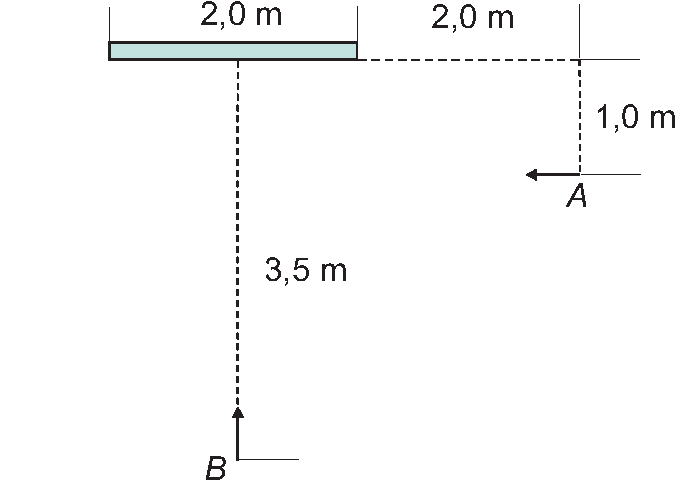
\includegraphics[width=0.5\linewidth]{2012-v2g-01-peegel2}%
\end{center}
\probend
\bigskip

% P108
\setAuthor{Tanel Kiis}
\setRound{lõppvoor}
\setYear{2013}
\setNumber{G 1}
\setDifficulty{3}
\setTopic{Geomeetriline optika}

\prob{Lenses}
\probeng
Juku has a large number of concave lenses and to find their focal lengths he constructed a simple diagram. He directed a laser ray of diameter $2R$, parallel to the optical axis, to the center of a convex lens with a known focal length $f_1$, after that the ray is converged on one point on the screen. If a concave lens of focal length $f_2$ is now positioned at equal distance from the convex lens and the screen, then the diameter of the laser ray on the screen is $2r$. Find $f_2$ assuming that $2f_2 < f_1$.
\probend
\bigskip

% P109
\setAuthor{Valter Kiisk}
\setRound{lõppvoor}
\setYear{2015}
\setNumber{G 2}
\setDifficulty{3}
\setTopic{Geomeetriline optika}

\prob{Lighting}
\probeng
A lens with a focal length $f_1=\SI{4}{cm}$ is positioned so that a parallel light beam of diameter $d_0=\SI{1}{cm}$ is focused at one point on the screen. Sometimes a bigger area is needed to be lighted on the screen but moving the lens or changing the source of the light is impossible. How big has to be the focal length $f_2$ of an additional lens positioned to the right of the initial lens, so that an evenly lighted area with a diameter $d=\SI{2}{cm}$ would appear on the screen? The distance between the lenses is $L$.
\begin{center}
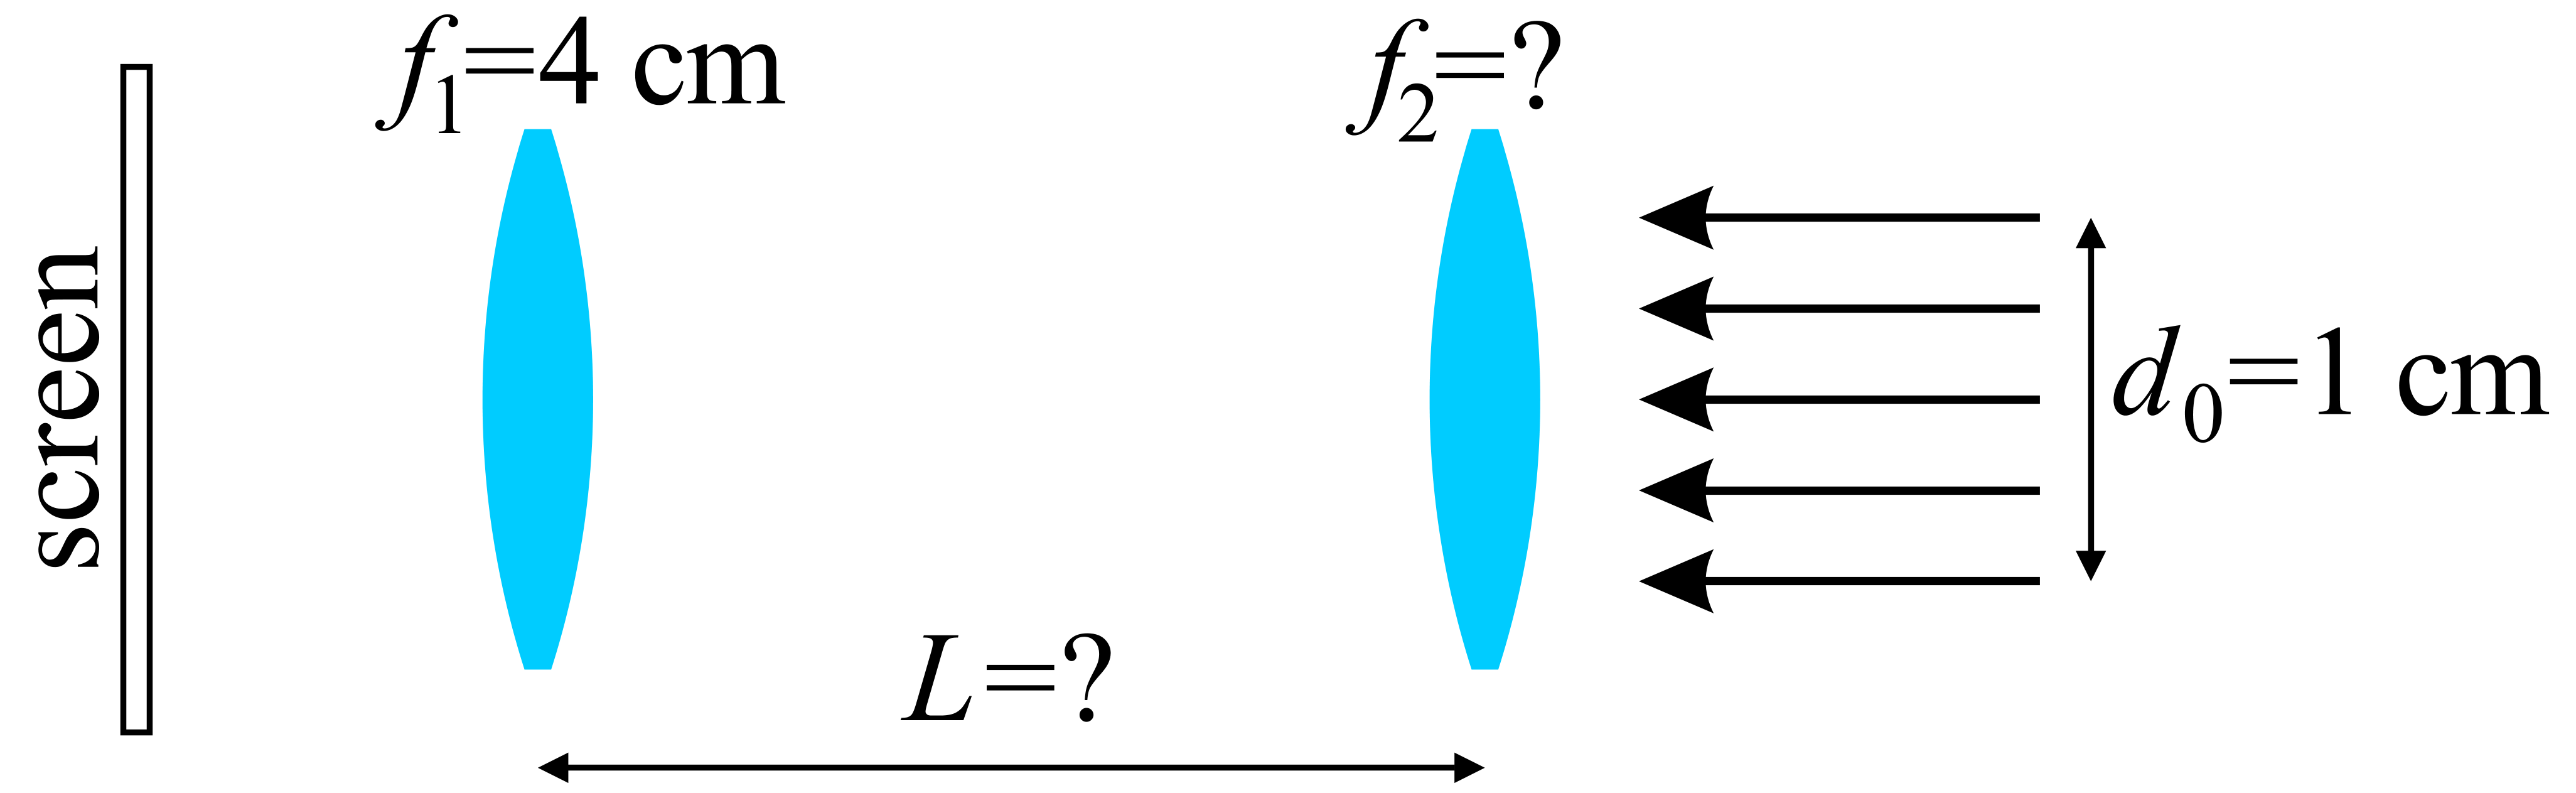
\includegraphics[scale=1.5]{2015-v3g-02-valgustamine-yles_ing}
\end{center}
\probend
\bigskip

% P110
\setAuthor{Andreas Valdmann}
\setRound{lahtine}
\setYear{2016}
\setNumber{G 4}
\setDifficulty{4}
\setTopic{Geomeetriline optika}

\prob{Optical fiber}
\probeng
An optical fiber consists of a cylindrical glass core with a refractive index $n_1=\SI{1,46}{}$ and a coating with a refractive index $n_2=\SI{1,44}{}$ that surrounds the core as a tube. Using classical optics, find the apex angle of a cone of light leaving a long optical fiber.
\probend
\bigskip

% P111
\setAuthor{Andres Põldaru}
\setRound{lahtine}
\setYear{2016}
\setNumber{G 5}
\setDifficulty{4}
\setTopic{Geomeetriline optika}

\prob{Three lenses}
\probeng
\begin{wrapfigure}[9]{r}{0.6\textwidth}
	\vspace{-20pt}
	\begin{resizebox}{0.6\textwidth}{!}{
\begin{tikzpicture}
\draw[{Stealth[scale=1.0]}-{Stealth[scale=1.0]}, line width=1pt] (0,0)-- ++(30:5);
\draw[{Stealth[scale=1.0]}-{Stealth[scale=1.0]}, line width=1pt] (30:5)-- ++(-90:5);%
\draw[{Stealth[scale=1.0]}-{Stealth[scale=1.0]}, line width=1pt] (0,0)-- ++(-30:5);
%\draw[->] (0,0) -- (5,0);
\node at (5.77,0) {\textbullet} (5.77,0) node[anchor=west] {$B$};
\node at (-2.89,0) {\textbullet} (-2.89,0) node[anchor=east] {$A$};
\draw[decorate,decoration={brace,raise=2pt,amplitude=6pt}] (0,0)  -- node[below right = 7pt and -10pt]{$2f$} (-2.89,0) ;
\draw[decorate,decoration={brace,raise=2pt,amplitude=6pt}] (5.77,0)  -- node[below right = 7pt and -8pt]{$f$} (4.33,0) ;
\end{tikzpicture}}
	\end{resizebox}
\end{wrapfigure}
Three lenses are put together so that they form an equilateral triangle. The lenses have one common focal point. A point light source is placed at the point A, which is at a distance $2f$ from the tip of the triangle, where $f$ is the focal length of the lenses. Explain by constructing on the draft whether a part of the light reaches the point B or not.
\probend
\bigskip

% P112
\setAuthor{Eero Vaher}
\setRound{piirkonnavoor}
\setYear{2017}
\setNumber{G 5}
\setDifficulty{4}
\setTopic{Geomeetriline optika}

\prob{Missing lens}
\probeng
A light originating from an object first goes through a concave lens and then a convex lens. The locations of the object, the convex lens and the forming image are shown in the figure, the focal points $F_k$ of the convex lens are also included. Construct the locations of the concave lens and the focal point $F_n$ that is closer to the object.\\
\begin{resizebox}{\linewidth}{!}{
		\begin{tikzpicture}
		\pgfmathsetmacro{\fk}{2}
		\pgfmathsetmacro{\tk}{3*\fk}
		\pgfmathsetmacro{\nk}{1/(1/\fk-1/\tk)}
		\pgfmathsetmacro{\a}{2*\fk}
		\pgfmathsetmacro{\h}{0.5}
		\pgfmathsetmacro{\htk}{\tk/\nk*\h}
		\pgfmathsetmacro{\ha}{1.5*\h}
		\pgfmathsetmacro{\nl}{\nk-\h/(\h-\ha)*(\nk-\a)}
		\pgfmathsetmacro{\fn}{\nk-\h/(\h-\ha)*(\nk-\nl)}
		\coordinate (TK) at (\tk, -\htk);
		\coordinate (NK) at (-\nk, \h);
		\coordinate (A) at (-\a, \ha);
		\draw (-1.1*\fn, 0) -- (1.1*\tk, 0);
		\draw[<->, ultra thick] (0,3.5*\h) -- (0,-3.5*\h);
		\draw[->, ultra thick] (\tk, 0) -- (TK);
		\draw[fill] (-\fk, 0) circle (0.02*\fk) node[below] {$F_k$};
		\draw[fill] (\fk, 0) circle (0.02*\fk) node[below] {$F_k$};
		\draw[->, ultra thick] (-\a, 0) -- (A);
		\end{tikzpicture}}
\end{resizebox}
\probend
\bigskip

% P113
\setAuthor{Andreas Valdmann}
\setRound{lõppvoor}
\setYear{2014}
\setNumber{G 4}
\setDifficulty{5}
\setTopic{Geomeetriline optika}

\prob{Periscope glasses}
\probeng
\begin{wrapfigure}{r}{0.38\textwidth}
  \begin{center}
    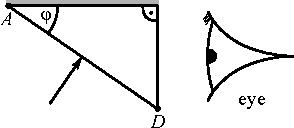
\includegraphics[width=0.4\textwidth]{2014-v3g-04-periskoopprillid_yl_joonis_ing}
  \end{center}
\end{wrapfigure}
Reading a book for too long is known to cause neck strain. To avoid this, a special pair of glasses were invented that do not require tilting the head to look down. The main element of these glasses is a prism shown in the figure. The upper face of the prism is covered with a material that reflects light. The apex angle $\varphi$ of the prism is chosen so that if the light ray entering the prism is perpendicular to the surface, then the ray that exits is also perpendicular. The prism is made of material with a refractive index $n=\SI{1,5}{}$.\\
a) On the line $AD$ there are points $B$ and $C$ that divide it into three sections: $AB$, $BC$ and $CD$. Depending on what section the ray falls on there are in principal three different routes in the prism for the ray. Make a draft of the ray’s routes for all the cases. \\
b) Find the value of $\varphi$.\\
c) Let the length of the side $AD$ be $l$. How far are the points $B$ and $C$ distanced from the tip $A$?\\
d) Why is this quite complex system used in the glasses instead of using a simple plane mirror to tilt the beams?
\probend
\bigskip

% P114
\setAuthor{Mihkel Kree}
\setRound{lahtine}
\setYear{2015}
\setNumber{G 5}
\setDifficulty{5}
\setTopic{Geomeetriline optika}

\prob{Lens}
\probeng
The figure shows an object AB and its real image A’B’ made by a convex lens. Find the locations of the lens’ center and the focal point, by construction.
\begin{center}
 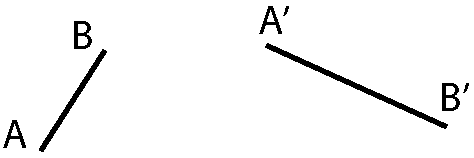
\includegraphics[width=0.7\linewidth]{2015-lahg-05-laatsMihkel}
\end{center}
\probend
\bigskip

% P115
\setAuthor{Sandra Schumann}
\setRound{lõppvoor}
\setYear{2018}
\setNumber{G 3}
\setDifficulty{5}
\setTopic{Geomeetriline optika}

\prob{Mirror base}
\probeng
A convex glass lens is placed at the bottom of an empty vessel with a mirror for the base so that the optical axis of the lens is perpendicular to the plane mirror. The distance between the lens and the base of the vessel is $l=\SI{10}{cm}$. A parallel light beam is directed on the lens and it converges at some point $A$ after going through the lens. Then the vessel is filled with water (the lens stays below the water). The beam is still converged at the point $A$. Find the focal length $f$ of the lens in air. \\
The refractive index of glass is $n_g = \SI{1,49}{}$, the refractive index of water is $n_w = \SI{1,33}{}$ and the refractive index of air is $n_0 = \SI{1,0}{}$. The refractive index shows how many times the speed of light in vacuum is bigger than in the substance. \\
\emph{Note.} For finding the focal length $f_w$ of a lens the following formula applies:
\[ f_w = f\cdot\frac{n_g n_w - n_0 n_w}{n_g n_0 - n_0 n_w}. \]
\probend
\bigskip

% P116
\setAuthor{Eero Vaher}
\setRound{piirkonnavoor}
\setYear{2015}
\setNumber{G 8}
\setDifficulty{6}
\setTopic{Geomeetriline optika}

\prob{Focal length}
\probeng
The left face of a thin lens is flat while the right face is concave and silvered. How big is the focal length $f$ of such an optical element for a light falling from the left? The radius of the lens’s concave part is $R$, the refractive index of the lens with respect to the surrounding environment is $n$.
\begin{center}
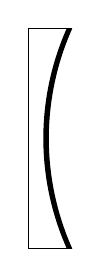
\begin{tikzpicture}[scale=0.7, transform shape]
\def\tmp{65.92}
\fill [black] (0.7,2) arc[start angle=90+\tmp, end angle=270-\tmp,radius=4.9] -- (0.8,-2) -- (0.8,-2) arc[start angle=270-\tmp, end angle=90+\tmp,radius=4.9] -- (0.7,2);
\draw (0.8,-2) -- (0,-2) -- (0,2) -- (0.8,2);
\end{tikzpicture}
\end{center}
\probend
\bigskip

% P117
\setAuthor{Jaan Kalda}
\setRound{lõppvoor}
\setYear{2012}
\setNumber{G 6}
\setDifficulty{7}
\setTopic{Geomeetriline optika}

\prob{Tube}
\probeng
A tube with reflecting inner walls has a point light source at the bottom of it (see figure). The inner diameter of the tube is $d=\SI{12}{mm}$, the tube’s length is $l=\SI{60}{mm}$. A convex lens with a focal length $F=\SI{36}{mm}$ is placed against the open end of the tube and at a distance $L=\SI{90}{mm}$ from the tip of the tube there is a screen, which has a graph paper attached to it. The intersection point with the optical axis $O$ is marked on the paper. Sketch the image that can be seen on the screen.
\begin{center}
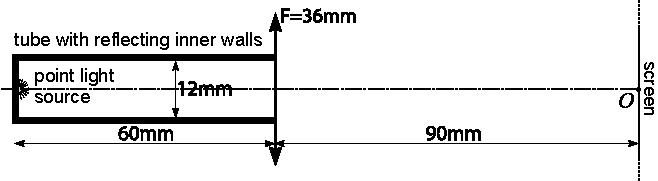
\includegraphics[width=\textwidth]{2012-v3g-06-toru-valgusallikas-lxxts_ing}
\end{center}
\probend
\bigskip

% P118
\setAuthor{Valter Kiisk}
\setRound{lõppvoor}
\setYear{2013}
\setNumber{G 7}
\setDifficulty{7}
\setTopic{Geomeetriline optika}

\prob{Microscope}
\probeng
A digital microscope consists of a lens that can be moved along the optical axis and produces a real image of an observable object on the surface of a matrix sensor. A sharp image appears in the case of two different positions of the lens. The ratio of the respective magnifying factors was determined to be 25. At what position and how many times is the radiated power per unit of area on the sensor bigger? You can assume that the dimensions of the lens are a lot smaller than its distance from the object.
\probend
\bigskip

% P119
\setAuthor{Erkki Tempel}
\setRound{lahtine}
\setYear{2014}
\setNumber{G 7}
\setDifficulty{7}
\setTopic{Geomeetriline optika}

\prob{Optical diagram}
\probeng
\begin{center}
  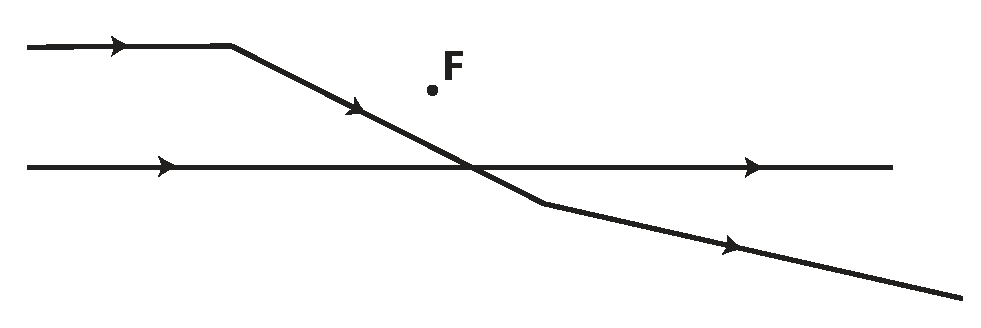
\includegraphics[width=0.7\textwidth]{2014-lahg-07-optilineskeemjoonis}
\end{center}
The figure depicts a route of two parallel beams through two identical convex lenses that are not parallel. The focal points of the lenses coincide at a point F. Construct the lenses with the optical axes on the figure.
\probend
\bigskip

% P120
\setAuthor{Valter Kiisk}
\setRound{lõppvoor}
\setYear{2016}
\setNumber{G 6}
\setDifficulty{7}
\setTopic{Geomeetriline optika}

\prob{Magnifier}
\probeng
If you place the flat side of a hemispherical glass object (lens) against a paper, it is possible to see a magnified image of the paper’s surface around the center of the lens. How many times is the image bigger than the object if you are observing at a distance that is much bigger than the dimensions of the lens? The refractive index of glass is $n=\num{1.5}$.
\probend
\bigskip

% P121
\setAuthor{Andreas Valdmann}
\setRound{lõppvoor}
\setYear{2016}
\setNumber{G 8}
\setDifficulty{8}
\setTopic{Geomeetriline optika}

\prob{Corner mirror}
\probeng
\begin{wrapfigure}{r}{0.3\textwidth}
	\vspace{-25pt}
	\begin{center}
		
\includegraphics[width=0.3\textwidth]{2016-v3g-08-wink}
	\end{center}
	\vspace{-20pt}
\end{wrapfigure}
Juku had three square-shaped plane mirrors for experimenting. Looking at one mirror and squeezing his right eye he saw the reflection depicted in the figure. Next, Juku positioned the three mirrors so that they formed the three faces of a cube that had a common tip. The reflecting faces of the mirrors stayed on the inner side of the cube. Sketch the reflection of himself that Juku saw while closing his right eye and looking exactly at the common vertex of the mirrors. Explain by construction.
\probend
\bigskip

% P122
\setAuthor{Jaan Kalda}
\setRound{lõppvoor}
\setYear{2015}
\setNumber{G 7}
\setDifficulty{9}
\setTopic{Geomeetriline optika}

\prob{Circle and eclipse}
\probeng
A ring and its image produced by a convex lens are depicted in the figure. Find the center of the lens, the optical axis and the focal point.
\begin{center}
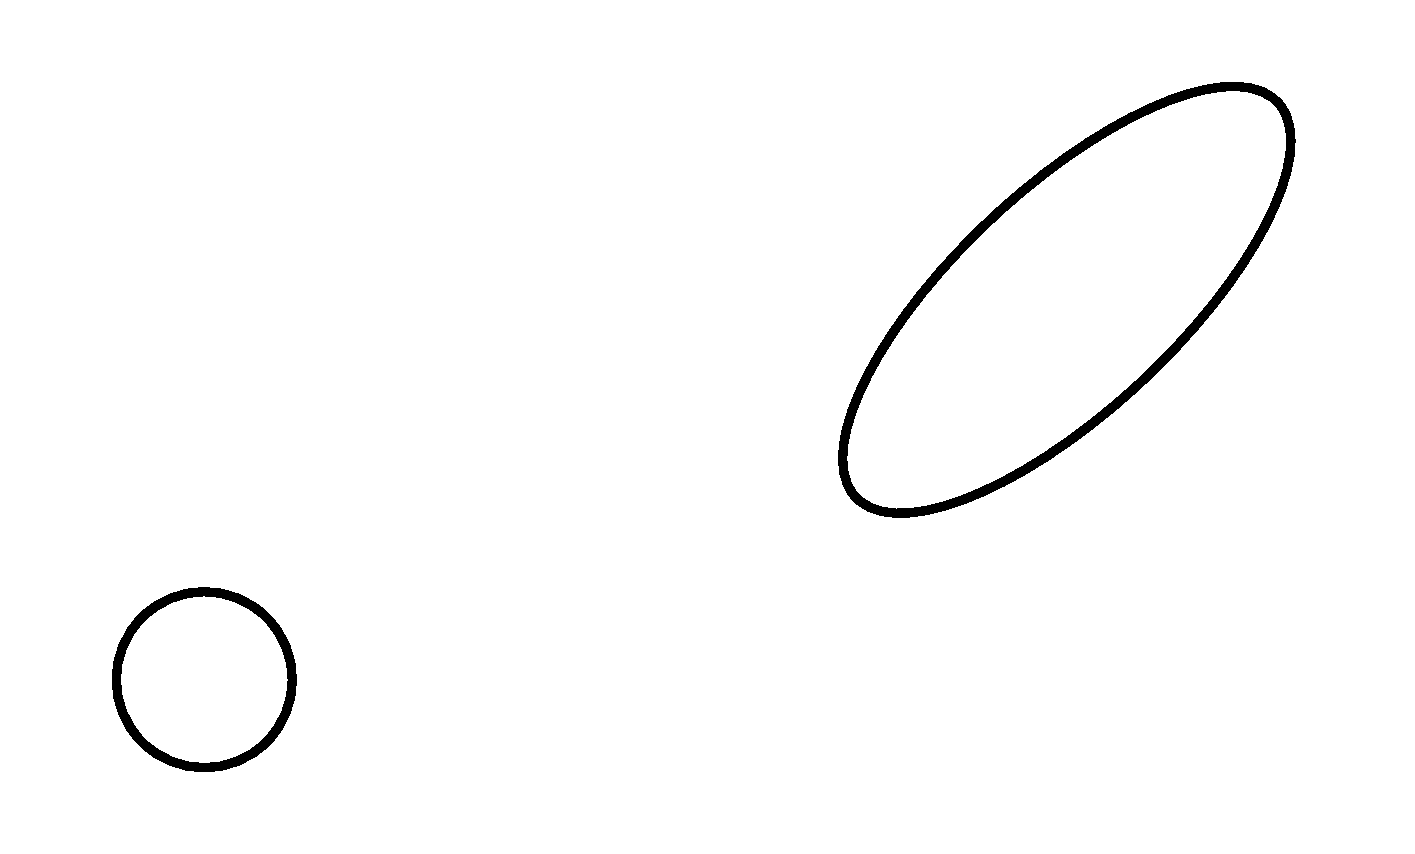
\includegraphics[width=0.7\textwidth]{2015-v3g-07-ringjaellips}%
\end{center}
\probend
\bigskip

% P123
\setAuthor{Ardi Loot}
\setRound{lõppvoor}
\setYear{2017}
\setNumber{G 8}
\setDifficulty{9}
\setTopic{Geomeetriline optika}

\prob{Camera}
\probeng
Juku is photographing northern lights with his self-built camera that consists of a square-shaped photosensitive element with a side length $2h=\SI{2.0}{cm}$ and a convex lens of focal length $f=\SI{14}{cm}.$. Juku does not like that the camera is so big and would prefer it to be maximally with a length $L_{m}=\SI{7.0}{cm}$ (the length of the camera is the distance between the photosensitive element and the outer lens). For that he installs a new convex lens of focal length $f_{2}=\SI{3.0}{cm}$ instead of the old one and he places it at the distance $L_{m}.$ from the photosensitive element. What should be the focal length of an additional concave lens in the system and its distance from the convex lens so that the initial camera’s field of view would be the same?
\probend
\bigskip

% P124
\setAuthor{Jaan Kalda}
\setRound{lõppvoor}
\setYear{2014}
\setNumber{G 10}
\setDifficulty{10}
\setTopic{Geomeetriline optika}

\prob{Glass cylinder}
\probeng
A point is marked on the outer surface of a glass cylinder. If that cylinder is observed at a great distance (much bigger than the radius of the cylinder), so that through the cylinder the point seems to be on the symmetry axis, then two additional images of the point can be seen. One point can be seen on one side of the symmetry axis, the second on the other side. If the cylinder were turned around its symmetry axis then at a particular moment those two points would merge together and disappear. The third image stays. If continuing to turn the cylinder, then at the moment when the angle of rotation with respect to the initial position is $\ang{15}$, the third image would disappear so that the marked point would not be seen anymore. How big is the refractive index of the glass?
\probend
\bigskip
\newpage\subsection{\protect\StrSubstitute{Kinematics}{-}{ }}

% P125
\setAuthor{Koit Timpmann}
\setRound{piirkonnavoor}
\setYear{2013}
\setNumber{G 1}
\setDifficulty{1}
\setTopic{Kinemaatika}

\prob{Train}
\probeng
A freight train passed through a road section between two stations with an average speed 36 km/h. Through 2/5 of the driving time the train was evenly accelerating, then through the next 2/5 it drove with a constant speed and through the last 1/5 it slowed down evenly. How big was the train’s maximal speed on the section between the two stations?
\probend
\bigskip

% P126
\setAuthor{Mihkel Kree}
\setRound{lahtine}
\setYear{2015}
\setNumber{G 1}
\setDifficulty{2}
\setTopic{Kinemaatika}

\prob{Train whistle}
\probeng
A train is linearly approaching a station with constant speed. The engine driver blows a whistle for $t_0=\SI{10}{s}$ but the station manager waiting for the train measures the time of the whistling to be $t_1=\SI{9}{s}$. Find the speed of the train $v$. The speed of sound in the air is $c=\SI{340}{m/s}$.
\probend
\bigskip

% P127
\setAuthor{Erkki Tempel}
\setRound{piirkonnavoor}
\setYear{2015}
\setNumber{G 1}
\setDifficulty{2}
\setTopic{Kinemaatika}

\prob{Freight train}
\probeng
Usually a freight train drives with a constant speed $v=\SI{72}{km/h}$ but this time its arrival to the station was late by $\Delta t=\SI{5}{min}$. Maintenance work was being done on the railways and the train had to drive with a speed $v_{h}=\SI{18}{km/h}$ for some time. The acceleration of the train while slowing down was $a_p=\SI{0,2}{m/s^2}$ and while speeding up $a_k=\SI{0,1}{m/s^2}$. For what distance did the train drive with the speed 18 km/h?
\probend
\bigskip

% P128
\setAuthor{Sandra Schumann}
\setRound{lahtine}
\setYear{2017}
\setNumber{G 1}
\setDifficulty{2}
\setTopic{Kinemaatika}

\prob{Ambulance}
\probeng
An ambulance drove by Juku on the street. Juku noticed that when the ambulance passed him the tone of its siren fell below by a minor third. How fast did the ambulance drive? Near Juku the speed of sound in the air was $v_h = \SI{343}{\meter\per\second}$. Assume that Juku’s distance from the linear trajectory of the ambulance is insignificantly small. The Doppler effect gives a relation between frequencies and velocities of motion.
\[ \frac{f_v}{f_a} = \frac{v_h + v_v}{v_h + v_a} \ , \] 
where \(f_v\) is the observed frequency, \(f_a\) the emitted frequency, \(v_v\) the velocity of the receiver and \(v_a\) the velocity of the source. \\
\emph{Hint.} Minor third is a musical interval that is a 3 semitone difference in a sound’s frequency. One octave means a 2 time difference in the sound’s frequency and is equal to 6 tones. Assume that the tones are divided in the octave so that if for three sound frequencies $f_1, f_2, f_3$ applies $\frac{f_2}{f_1} = \frac{f_3}{f_2}$ and if between $f_1$ and $f_2$ there is one tone then between $f_2$ and $f_3$ there is also one tone.
\probend
\bigskip

% P129
\setAuthor{Mihkel Rähn}
\setRound{piirkonnavoor}
\setYear{2017}
\setNumber{G 2}
\setDifficulty{2}
\setTopic{Kinemaatika}

\prob{Braking}
\probeng
Two cars are driving after one another with speed $v=\SI{50}{km/h}$. The first car brakes maximally, seeing that the first car brakes the car in the back also brakes maximally. The brakes of the first car are put to use at the exact same time when the brake lights turn on. It takes the rear car $t=\SI{1,5}{s}$ to apply the brakes from the moment when the front car’s brake lights turn on. Coefficient of friction is $\mu=1$ and gravitational acceleration $g=\SI{9,8}{m/s^2}$.\\
a) How big should the distance be between the two cars be while driving so that when braking there would be no collision?\\
b) If the distance between the cars is $l=\SI{5}{m}$ before the braking then how big is the speed difference between the cars at the moment of the collision?
\probend
\bigskip

% P130
\setAuthor{Jaan Kalda}
\setRound{lõppvoor}
\setYear{2013}
\setNumber{G 3}
\setDifficulty{4}
\setTopic{Kinemaatika}

\prob{Cyclist}
\probeng
A boy is measuring the speed of wind with respect to himself while riding on a bicycle: if he is riding along the road at one direction with a speed 10 km/h then he gets the result 20 km/h and if he rides the opposite direction with a speed 20 km/h then he also gets the result 20 km/h. How fast with respect to the ground is the wind blowing?
\probend
\bigskip

% P131
\setAuthor{Jaan Toots}
\setRound{lõppvoor}
\setYear{2014}
\setNumber{G 2}
\setDifficulty{4}
\setTopic{Kinemaatika}

\prob{Violin}
\probeng
If pressing down on a violin string with a length $L$ at a distance $\frac{3}{7}L$ from one end and dragging along the shorter part with a violin bow, a sound with fundamental frequency will be heard. When just touching the string at the same distance $\frac{3}{7}L$ (without pressing down) the sound heard is different. What is the ratio of these two fundamental frequencies?
\probend
\bigskip

% P132
\setAuthor{Taavi Pungas}
\setRound{piirkonnavoor}
\setYear{2012}
\setNumber{G 4}
\setDifficulty{5}
\setTopic{Kinemaatika}

\prob{Revolving stage}
\probeng
Often a part of a stage’s floor is a rotating disc. With a time $t$, an actor wishes to reach from a point $A$ beside the disc to another point beside the disc that would be as far as possible from $A$.  Where is such a target point $B$ positioned? Express the answer as an angle $\alpha = \angle \mathit{AOB}$ where $O$ is the center of the disc. The actor is walking with a speed $v$, the rotation period of the disc is $T$ and the radius $r$. You can assume that $\alpha < \ang{180}$.
\probend
\bigskip

% P133
\setAuthor{Eero Vaher}
\setRound{lõppvoor}
\setYear{2015}
\setNumber{G 5}
\setDifficulty{5}
\setTopic{Kinemaatika}

\prob{Ball throw}
\probeng
Juku is living in a cylindrical space station that rotates so that artificial gravitational force is created. The radius of the station is $R$, its rotation’s angular velocity is $\omega$. Juku throws a ball straight up with an initial speed $v=\frac{\sqrt{3}}{3}\omega R$. From how far away from Juku along the surface of the station will the ball land?
\probend
\bigskip

% P134
\setAuthor{Siim Ainsaar}
\setRound{lõppvoor}
\setYear{2012}
\setNumber{G 5}
\setDifficulty{6}
\setTopic{Kinemaatika}

\prob{Tires}
\probeng
For a car’s tires to wear as little as possible, the car should be built so that the front wheels would turn by a different angle on a curve. Find the best angle of rotation $\beta$ for the right front wheel on a right curve if the angle for the left front wheel is $\alpha$. The distance between the wheels longitudinally is $a$ and laterally is $b$ (see figure).
\begin{center}
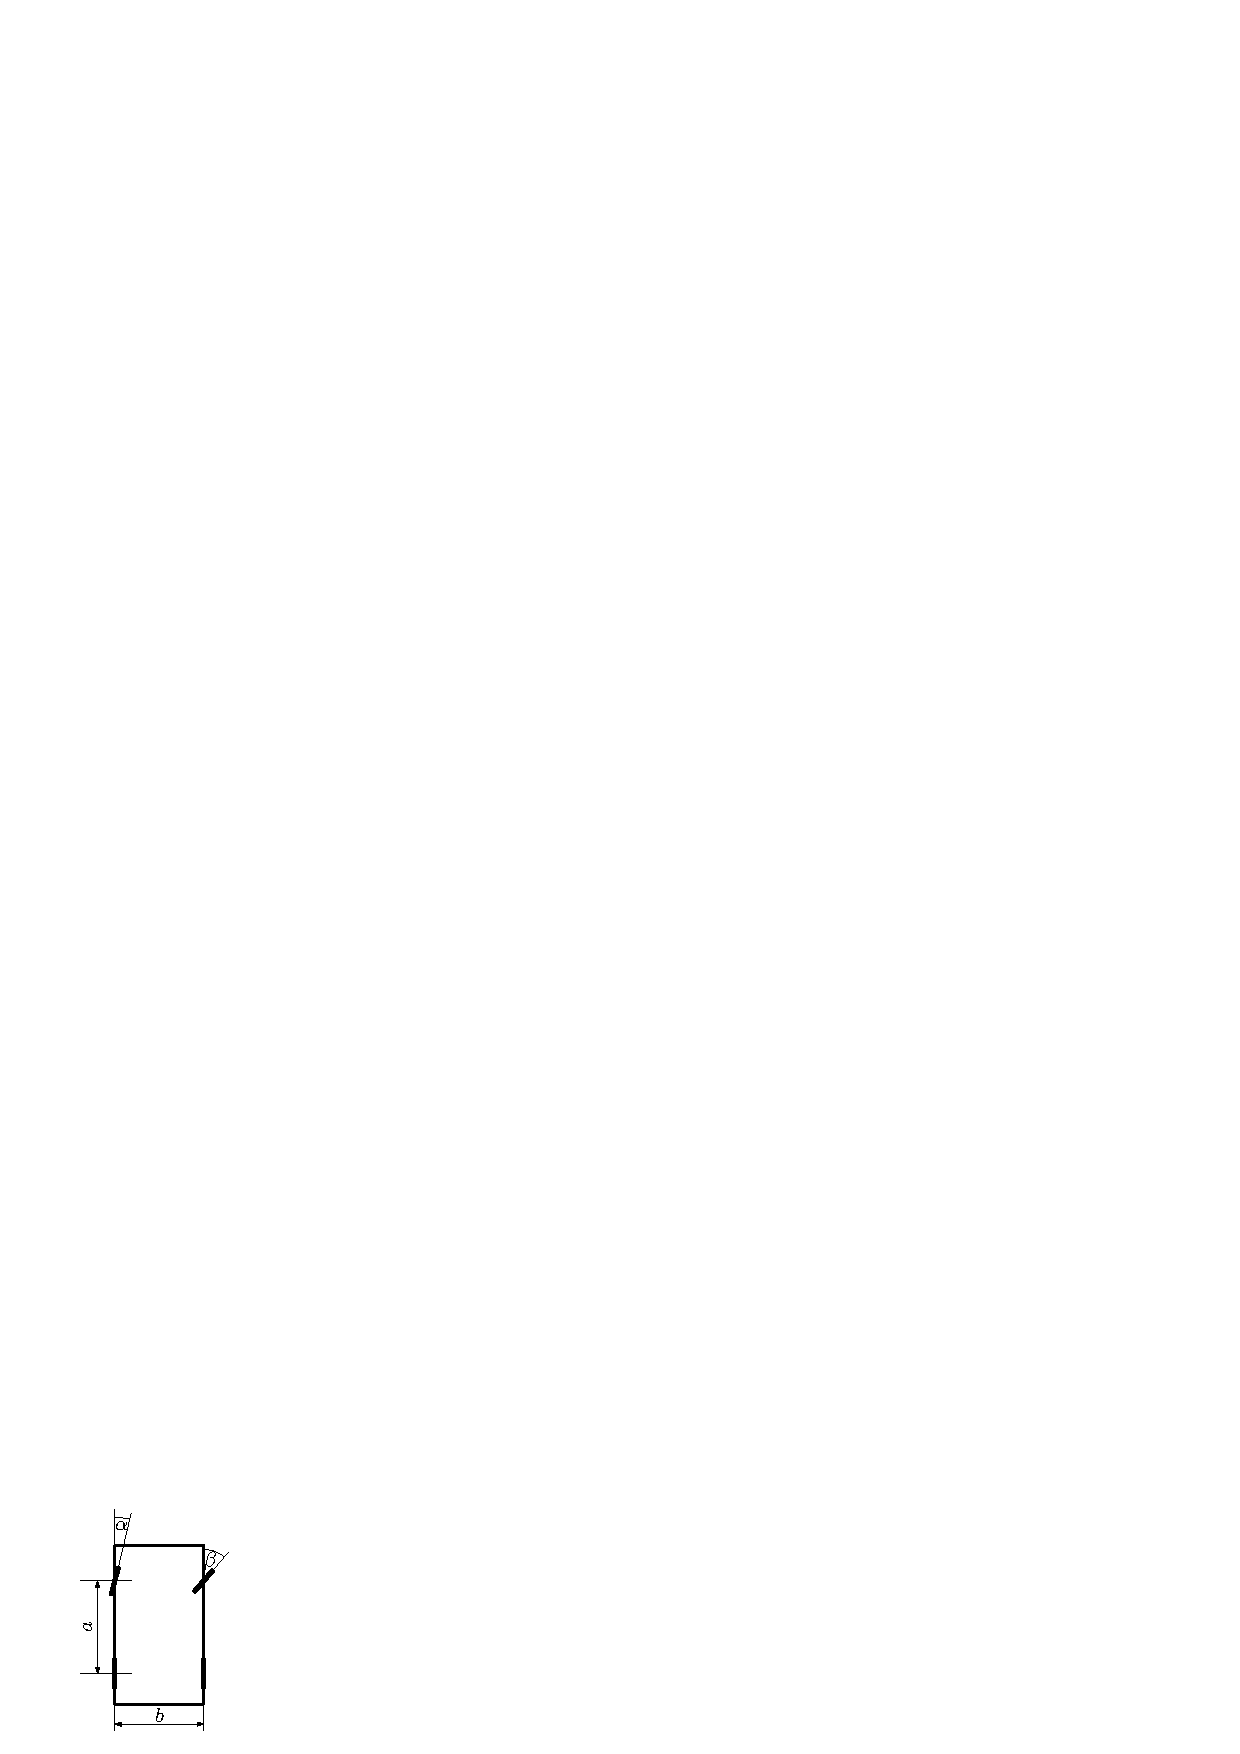
\includegraphics[width=0.3\linewidth]{2012-v3g-05-r_yl_joonis}%
\end{center}
\probend
\bigskip

% P135
\setAuthor{Jaan Kalda}
\setRound{lõppvoor}
\setYear{2014}
\setNumber{G 5}
\setDifficulty{6}
\setTopic{Kinemaatika}

\prob{Combs}
\probeng
Two combs are placed behind each other as in the figure. The grey comb is moved with a speed $v=\SI 1{cm/s}$ and the black comb is held still.  With what speed and to what direction are the dark spots moving?
\begin{center}
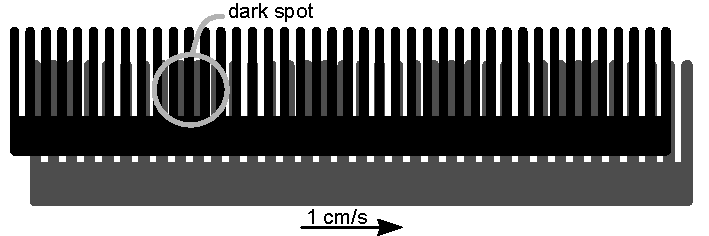
\includegraphics[width=0.6\textwidth]{2014-v3g-05-kammid_ing}
\end{center}
\probend
\bigskip

% P136
\setAuthor{Mihkel Kree}
\setRound{lahtine}
\setYear{2014}
\setNumber{G 10}
\setDifficulty{8}
\setTopic{Kinemaatika}

\prob{Rotation of the Sun}
\probeng
Earth is rotating around its axis with a period $T_\text{m}\approx\SI{24}{h}$. The Sun is also rotating around its axis. That can be proven for example by observing the motion of sunspots but in this exercise we use the information of the spectrums radiated by equatorial points A and B located on the edge of the Sun’s disc. It turns out that measuring the wavelengths of sodium’s yellow absorption line yields slightly different values for the points A and B. The measured wavelengths differ from each other by $\Delta \lambda = \SI{7.8}{pm}=\SI{7.8e-12}{m}$. The laboratory measured wavelength of sodium’s yellow absorption line is $\lambda_0=\SI{590}{nm}$, the speed of light $c=\SI{3.0e8}{m/s}$, the Sun’s radius $r=\SI{700000}{km}$. Find the rotation period $T_\text{p}$ of the Sun’s equatorial area.
\probend
\bigskip

% P137
\setAuthor{Jaan Kalda}
\setRound{lõppvoor}
\setYear{2014}
\setNumber{G 9}
\setDifficulty{8}
\setTopic{Kinemaatika}

\prob{Wire rings}
\probeng
Consider two identical rings made of wire with a radius $R$. The planes of the rings are parallel and the rings are touching each other at points $A$ and $B$. The central angle for the arc $AB$ is observable at a moment of time $\alpha$. The lower ring is still, the upper is rotating with an angular velocity $\omega$ around the axis that intersects with the point $A$ and that is perpendicular to the planes of the rings. Find the speed of the point $B$ at the given moment of time.
\probend
\bigskip

% P138
\setAuthor{Jaan Kalda}
\setRound{lahtine}
\setYear{2016}
\setNumber{G 9}
\setDifficulty{9}
\setTopic{Kinemaatika}

\prob{Anemometer}
\probeng
An ultrasonic anemometer measures wind speed by determining the time it takes for an audio signal to reach the sensors from an audio source. Let the audio source be at the origin $O=(0;0)$ and three sensors at points with the coordinates $A=(0;a)$, $B=(a;0)$ and $C=(-a;0)$ where $a=\SI{211.1}{mm}$ (let us make a simplifying assumption that the dimensions of both the audio source and the sensors are negligible). The anemometer is held so that all the sensors are located on the same horizontal plane and the times taken for the audio signal to reach the sensors are measured to be accordingly $t_A=\SI{627,0}{\micro s}$, $t_B=\SI{625,2}{\micro s}$ and $t_C=\SI{603,4}{\micro s}$. What is the speed of wind? You can use reasonable simplifying approximations for the calculations.
\probend
\bigskip

% P139
\setAuthor{Jaan Kalda}
\setRound{lõppvoor}
\setYear{2016}
\setNumber{G 9}
\setDifficulty{9}
\setTopic{Kinemaatika}

\prob{Motorboat}
\probeng
A motorboat was driving to an island located directly towards the South at a distance $l=\SI 4{km}$. Initially the direction was set on the first navigation mark, next it was set on the second mark and finally the course was set directly towards the island. Thus the route consisted of three straight lines. The speed and the direction of the wind was measured on the boat. The time it took to drive through the first section was $t_1=\SI{3}{min}$, the speed of the wind was measured to be $v_1=\SI{15}{m/s}$ and the perceived direction was directly from the East. The second section was driven in time $t_2=\SI{1,5}{min}$, the speed of the wind was $v_2=\SI{10}{m/s}$ and the perceived direction was directly from South-East. The third section was driven in time $t_3=\SI{1,5}{min}$, the speed of the wind was $v_3=\SI{5}{m/s}$ and the perceived direction was directly from South-West. What was the actual speed of the wind?\\
\emph{Note.} At different sections the speed of the boat may have been different but during one section the speed was constant. The time it took to turn and accelerate is negligible. The actual speed and direction of the wind did not change.
\probend
\bigskip
\newpage\subsection{\protect\StrSubstitute{Magnetism}{-}{ }}

% P140
\setAuthor{Kristian Kuppart}
\setRound{lahtine}
\setYear{2013}
\setNumber{G 2}
\setDifficulty{3}
\setTopic{Magnetism}

\prob{Magnet mirror}
\probeng
A particle with a positive charge $q$ and velocity $v$ moves towards a rectangular strip so that that its velocity vector forms an angle $\alpha$ with the normal of the strip. The thickness of the strip is $d$ and on it is located a homogeneous $z$-directional magnetic field with an induction $B$ (from the plane of the paper directed towards us). For what maximal falling angle $\alpha_{\mathrm{max}}$ does the particle still go through the magnetic field? It is known that the particle that enters the strip perpendicularly would go through the strip.
\begin{center}
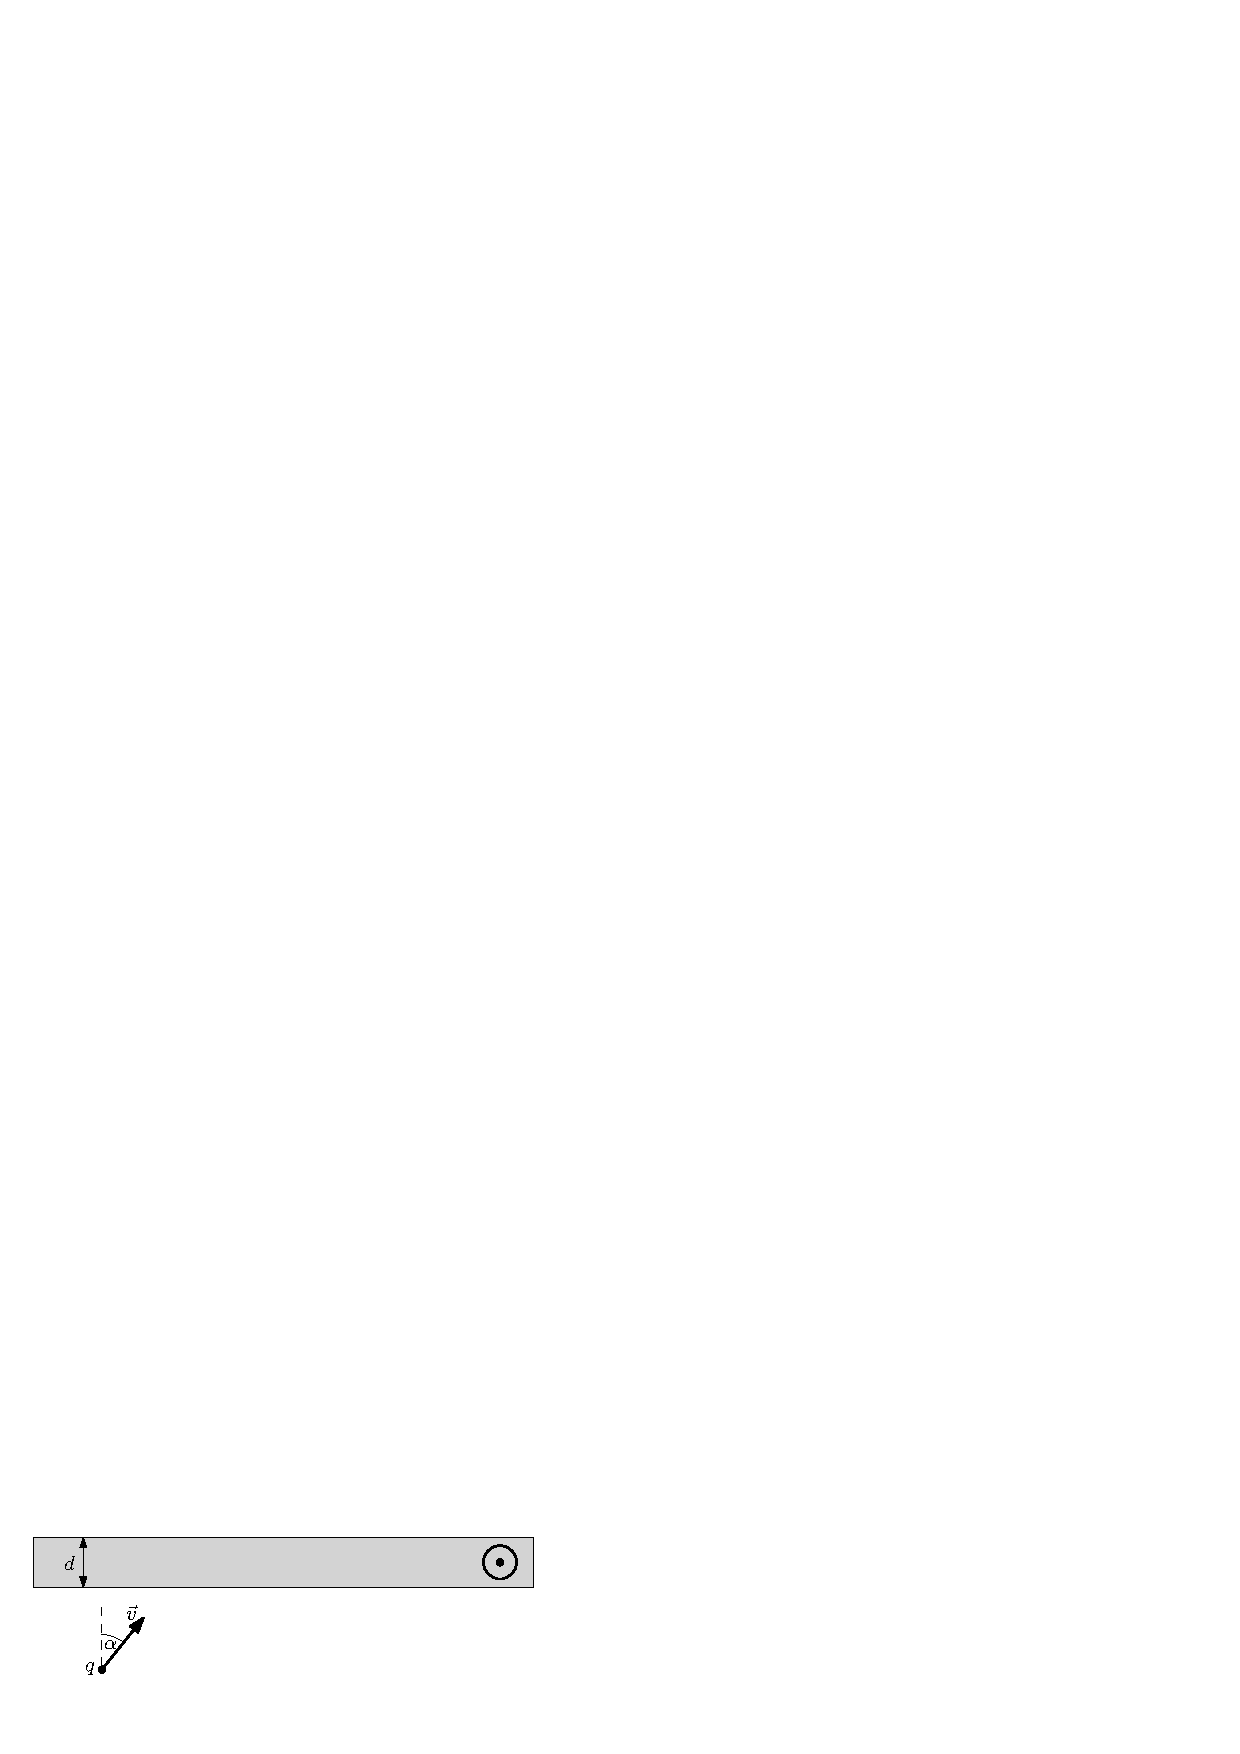
\includegraphics[width=\linewidth]{2013-lahg-02-magnetpeegeljoonis_ipe}
\end{center}
\probend
\bigskip

% P141
\setAuthor{Andreas Valdmann}
\setRound{lahtine}
\setYear{2013}
\setNumber{G 5}
\setDifficulty{4}
\setTopic{Magnetism}

\prob{Generator}
\probeng
In a certain type of electric generator there is a rotating wire contour connected to the output. The contour is rotating in a magnetic field created by a permanent magnet changing the mechanical work to electrical energy. An electrical lamp was connected to such a generator as an energy consumer. Initially the generator was rotating with an angular velocity $\omega_0$ which caused a power $P_0$ to emit from the lamp. At a certain moment the speed of rotation was increased by 2 times.\\
a) How big was the power emitted from the lamp after increasing the speed of rotation?\\
b) How big was the torque necessary to rotate the generator before and after changing the speed of rotation?\\
You can assume that the generator worked without any losses meaning that all the work done by the rotation was transferred to the lamp. When the speed of the rotation is even the torque causing the rotation of the generator is constant. You can also assume that the power of the lamp does not depend on the strength of the current going through it.
\probend
\bigskip

% P142
\setAuthor{Eero Vaher}
\setRound{lahtine}
\setYear{2013}
\setNumber{G 6}
\setDifficulty{5}
\setTopic{Magnetism}

\prob{Revolving ball}
\probeng
Let there be a positively charged ball of mass $m$. It is known that if the ball would move with a speed $v$ in a perpendicular magnetic field of induction $B$ then the ball’s trajectory would be a circle of radius $r$. How big should be the charge $q$ of another ball with the same mass so that the first ball would move with the same speed on the same trajectory in the electric field of the second ball? Assume that no external forces are applied to this system of two balls. All the movements are observed in a laboratory frame of reference.
\probend
\bigskip

% P143
\setAuthor{Kristian Kuppart}
\setRound{piirkonnavoor}
\setYear{2018}
\setNumber{G 10}
\setDifficulty{6}
\setTopic{Magnetism}

\prob{Cyclotron}
\probeng
\begin{wrapfigure}{r}{0.35\linewidth}
	\begin{center}
		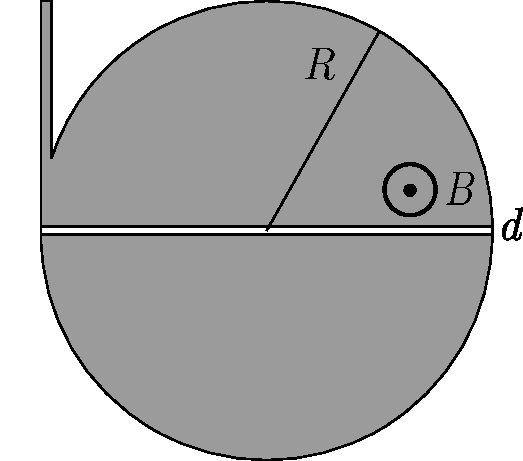
\includegraphics[width=\linewidth]{2018-v2g-10-tsyklotron}
	\end{center}
\end{wrapfigure}
Let us look at a cyclotron (a certain type of particle accelerator) and its activity. The cyclotron consists of a cylindrical region of radius $R$ where there is a homogeneous magnetic field of strength $B$ and a thin strip-shaped region of width $d$ where there is a homogenous electric field of strength $E$ perpendicular to the strip. The direction of the electrical field is changed periodically to be the opposite direction so that for every particle going through the strip the direction of the electric field is the same as the direction of the particle’s velocity. There is also a narrow canal at one edge of the cyclotron for the particles to exit the cyclotron. Let the particles start their movement at the center of the cyclotron with an insignificantly small initial speed. How many full circles $n$ will the particles make before leaving the cyclotron? The charge of the particles is $q$ and the mass $m$. Assume that $n\gg 1.$.
\probend
\bigskip

% P144
\setAuthor{Kristian Kuppart}
\setRound{piirkonnavoor}
\setYear{2013}
\setNumber{G 10}
\setDifficulty{7}
\setTopic{Magnetism}

\prob{Mass spectrometer}
\probeng
\begin{wrapfigure}[4]{r}{3cm}%
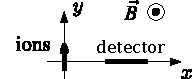
\includegraphics[width=\linewidth]{2013-v2g-10-massspektromeeter_ipe_ing}%
\end{wrapfigure}
In a laboratory there was a quantity of a substance to be examined. The molar mass of the substance was measured to be $\mu_{1}$. The substance was ionized once (each atom lost one electron), then accelerated in an electric field with a potential difference $U$ and directed to a magnetic field of induction $B$ (see figure). The magnetic induction was perpendicular to the plane of the figure, the initial velocity of the ions was $y$-directional, the magnetic field was located in the region $y>0$ and the substance entered the magnetic field at the origin, $(0, 0, 0)$.\\
It was observed that a small amount of the substance fell by a distance $d$ further on the detector on the $x$-axis from where the rest of the substance fell on. From this it was assumed that a small amount of the isotope in the substance had a different molar mass. Find the molar mass $\mu_{2}$ of this isotope. The Avogadro number is $N_A$ and the charge of an electron is $-e$.
\probend
\bigskip

% P145
\setAuthor{Jaan Kalda}
\setRound{piirkonnavoor}
\setYear{2015}
\setNumber{G 9}
\setDifficulty{8}
\setTopic{Magnetism}

\prob{Magnetic field}
\probeng
In the region $0<y<a$ there is a $z$-directional homogenous magnetic field with an induction $B$, in the regions $y<0$ and $y>a$ there is no magnetic field. A particle with a mass $m$ and a charge $q$ enters the magnetic field with a speed $v$ parallel to the $y$-axis over the line $y=0$. Sketch the angle between the particle’s velocity and the $y$-axis after when the particle has exited the region $0<y<a$ as a function of the speed $v$.
\probend
\bigskip

% P146
\setAuthor{Eero Vaher}
\setRound{lahtine}
\setYear{2015}
\setNumber{G 10}
\setDifficulty{9}
\setTopic{Magnetism}

\prob{Charged pendulum}
\probeng
A small charged ball of mass $m$ and charge $q$ is hanging at the end of a non-stretchable thread of length $l$ in a magnetic field of induction $B$. The ball is brought to a height $H=\frac{7}{8}l$ while holding the thread straight and then it is let free. The gravitational acceleration is $g$ and the direction of the magnetic field is perpendicular to the plane of the pendulum. It is also known that $q^2B^2l=\frac{3}{4}m^2g$ applies. What is the trajectory of the ball?
\begin{center}
\begin{resizebox}{0.5\linewidth}{!}{
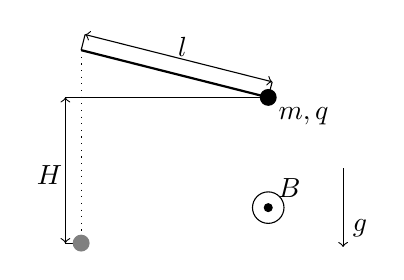
\begin{tikzpicture}
\newcommand{\x}{1.2*1.98}
\newcommand{\y}{-0.6}
\newcommand{\length}{{veclen(\x,\y)}}

\draw (\x,-2) circle (0.2) node [above right] {$B$};
\draw[fill=black] (\x, -2) circle (0.05);
\draw[->] (1.4*\x,-1.5) -- (1.4*\x,-2.5) node[above right] {$g$};

\draw[<->] (0.05,-0.05*\x/\y) -- (\x+0.05,\y-0.05*\x/\y);
\draw (0,0) -- (0.05,-0.05*\x/\y);
\draw (\x,\y) -- (\x+0.05,\y-0.05*\x/\y);
\draw[thick] (0,0) -- (\x,\y) node[below right] {$m,q$};
\draw[fill=black] (\x,\y) circle (0.1);
\node[above] at (\x/2+0.1,\y/2+0.1) {$l$};

\draw[<->] (-0.2,\y) -- (-0.2,-\length);
\draw (\x,\y) -- (-0.2,\y);
\draw (0,-\length) -- (-0.2,-\length);
\draw[dotted] (0,0) -- (0,-\length);
\draw[gray, fill=gray] (0,-\length) circle (0.1);
\node[left] at (0,-\length/2.5+\y) {$H~$};
\end{tikzpicture}}
\end{resizebox}
\end{center}
\probend
\bigskip

% P147
\setAuthor{Jaan Kalda}
\setRound{lõppvoor}
\setYear{2017}
\setNumber{G 10}
\setDifficulty{10}
\setTopic{Magnetism}

\prob{Electrons}
\probeng
At a region of space $x>-a$ ($a>0$) there is a homogenous $z$-directional magnetic field of induction $B$. At the origin there is a source of electrons that radiates electrons equally to all directions (over a solid angle $4\pi$). The speed of all the electrons is $v$. At the plane $x=-a$ there is a screen. If the electrons of charge $e$ and mass $m$ hit the screen, then there is light seen at the point of the collision. Find the $y$-directional diameter of the glowing spot on the plane $z = 0$, assuming that at least some of the electrons reach the screen. At the same plane, find where is the biggest luminous intensity of the spot. What is the $z$-directional length of the spot on the plane $y=0$?
\probend
\bigskip
\newpage\subsection{\protect\StrSubstitute{Statics}{-}{ }}

% P148
\setAuthor{Taavi Pungas}
\setRound{piirkonnavoor}
\setYear{2014}
\setNumber{G 6}
\setDifficulty{4}
\setTopic{Staatika}

\prob{Ring}
\probeng
A plastic ring of radius $L$ is attached to the ceiling with a rope of length $R$. A heavy metal nut is in turn attached to the ring. The nut can be slided along the ring. The coefficient of friction between the nut and the ring is $\mu$. While sliding the nut along the ring Juku wants to achieve a situation where the distance $h$ between the nut and the ceiling would be as small as possible but that the system would still be in equilibrium. Find the smallest distance $h\idx{min}$ that Juku can achieve. Assume that the mass of the ring is insignificantly small compared to the mass of the nut.
\probend
\bigskip

% P149
\setAuthor{Mihkel Rähn}
\setRound{piirkonnavoor}
\setYear{2015}
\setNumber{G 7}
\setDifficulty{5}
\setTopic{Staatika}

\prob{Bolt cutter}
\probeng
Find how much force does the blade of the bolt cutter apply on the bolt (see figure) if the force applied on the handle is $F = \SI{90}{N}$.
\begin{center}
    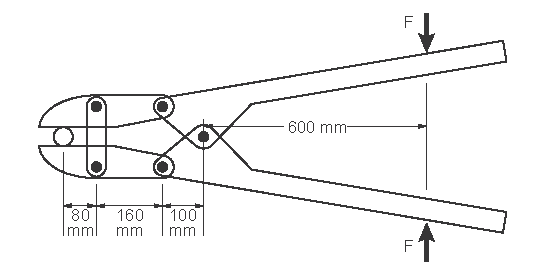
\includegraphics[width=0.7\textwidth]{2015-v2g-07-poldiloikur}
  \end{center}
\probend
\bigskip

% P150
\setAuthor{Mihkel Rähn}
\setRound{piirkonnavoor}
\setYear{2014}
\setNumber{G 7}
\setDifficulty{6}
\setTopic{Staatika}

\prob{Block}
\probeng
On a horizontal table there is a block of mass $m_1$ and on top of it is placed another block of mass $m_2$. The coefficient of static friction between the two blocks is $\mu_2$. The coefficient of kinetic friction between the bottom block and the table is $\mu_1$. Find the maximal horizontal force $F$ that can be used to pull the bottom block without the upper block starting to slide.
\probend
\bigskip

% P151
\setAuthor{Mihkel Rähn}
\setRound{lõppvoor}
\setYear{2014}
\setNumber{G 6}
\setDifficulty{6}
\setTopic{Staatika}

\prob{Polyspast}
\probeng
A polyspast is made from convenient tools (three blocks and parts of rope) to pull out an alpinist who fell into an ice gap. The main rope is marked with a thick line in the simplified figure, the fallen alpinist is attached to one end and the other end is pulled at. The blocks are attached to the main rope with a non-sliding knot with the help of ropes that are depicted as thin lines in the figure. Find the transmission factor of the polyspast while not accounting for the friction and also for the case where it is assumed that the friction decreases the force transmission by $\SI{35}{\percent}$ for each block. Assume that all the forces are vertical.
\begin{center}
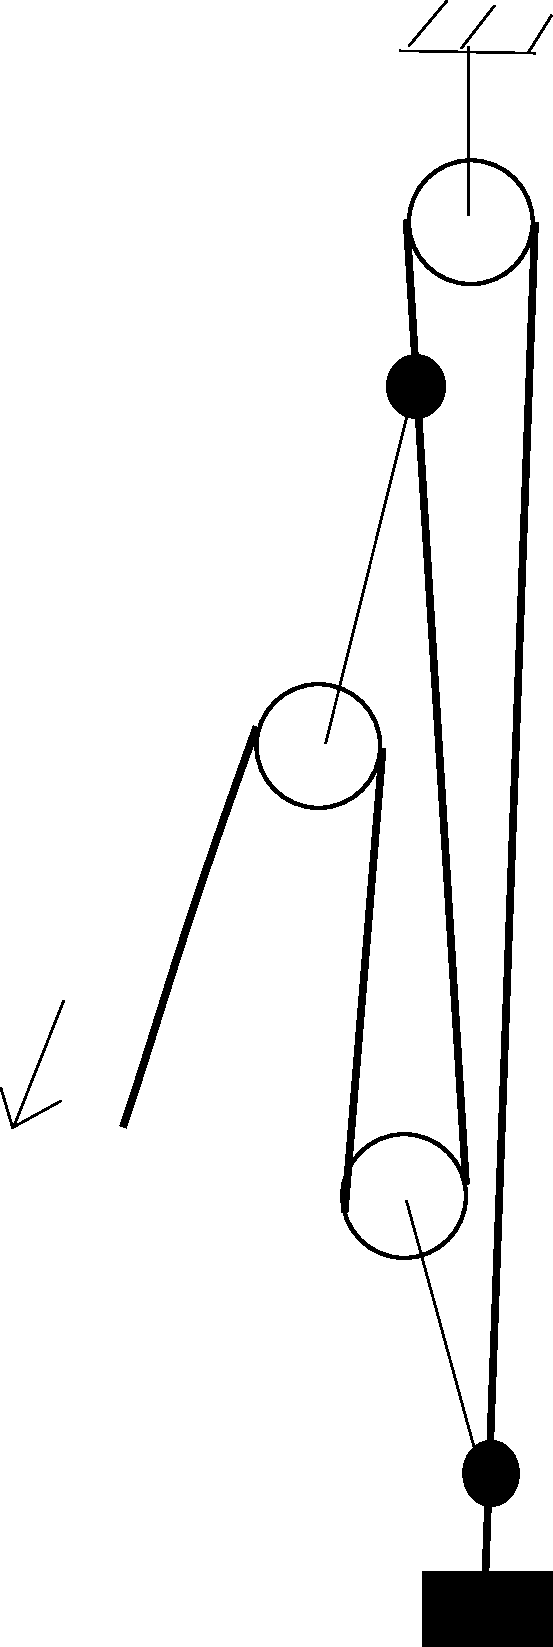
\includegraphics[width=0.25\linewidth]{2014-v3g-06-Polyspast}
\end{center}
\probend
\bigskip

% P152
\setAuthor{Andreas Valdmann}
\setRound{piirkonnavoor}
\setYear{2018}
\setNumber{G 9}
\setDifficulty{6}
\setTopic{Staatika}

\prob{Sledge}
\probeng
Juku went sledging with his friends. When going back, two of Juku’s friends sat on his sledge and Juku tried to pull the sledge after him on a horizontal and snowy road. What is the minimal angle between the rope of the sledge and the ground so that it is possible for Juku to pull the sledge into motion? Juku’s mass is $m_1 = \SI{60}{kg}$ and the coefficient of friction between Juku’s boots and the snow is $\mu_1 = \SI{0.30}{}$. The mass of the sledge together with Juku’s friends is $m_2 = \SI{110}{kg}$ and the coefficient of friction between the sledge and the snow is $\mu_2 = \SI{0.20}{}$.
\probend
\bigskip

% P153
\setAuthor{Mihkel Kree}
\setRound{lahtine}
\setYear{2013}
\setNumber{G 8}
\setDifficulty{7}
\setTopic{Staatika}

\prob{Thread roll}
\probeng
\begin{wrapfigure}[6]{r}{3cm}
\vspace{-15pt}
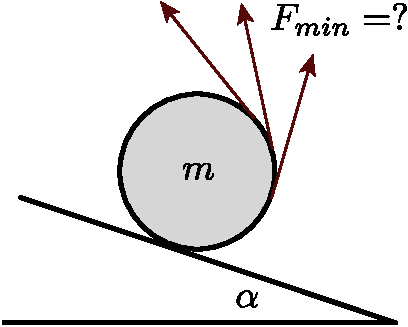
\includegraphics[width=\linewidth]{2013-lahg-08-joonis_niidirull-crop}
\end{wrapfigure}
A cylinder of mass $m$ has a thin thread winded over it and it is placed on an inclined surface with an inclination angle of $\alpha$. What is the required minimal force $F\idx{min}$ to hold the thread so that the cylinder would stay still (see figure)? The coefficient of friction between the surface and the cylinder is so big that there is no sliding.
\probend
\bigskip

% P154
\setAuthor{Andres Põldaru}
\setRound{lahtine}
\setYear{2014}
\setNumber{G 8}
\setDifficulty{7}
\setTopic{Staatika}

\prob{Cyclist}
\probeng
A cyclist is riding down a slope with an even inclination. If he is holding the brakes with exactly such a strength to cause the rear wheel to almost rise into air, then his speed while riding down the slope does not change. The center of mass of the system that consists of the cyclist and the bike is located exactly in the middle of two wheels, at a height $h$ from the ground. The distance between the axes of the wheels is $d$. How big is the angle $\alpha$ between the slope and the horizontal direction? How big has to be the coefficient of friction $\mu$ between the wheel and the ground so that the cyclist could brake like it was described?
\probend
\bigskip

% P155
\setAuthor{Stanislav Zavjalov}
\setRound{lahtine}
\setYear{2012}
\setNumber{G 9}
\setDifficulty{9}
\setTopic{Staatika}

\prob{Rope in groove}
\probeng
\begin{wrapfigure}{r}{0.4\linewidth}
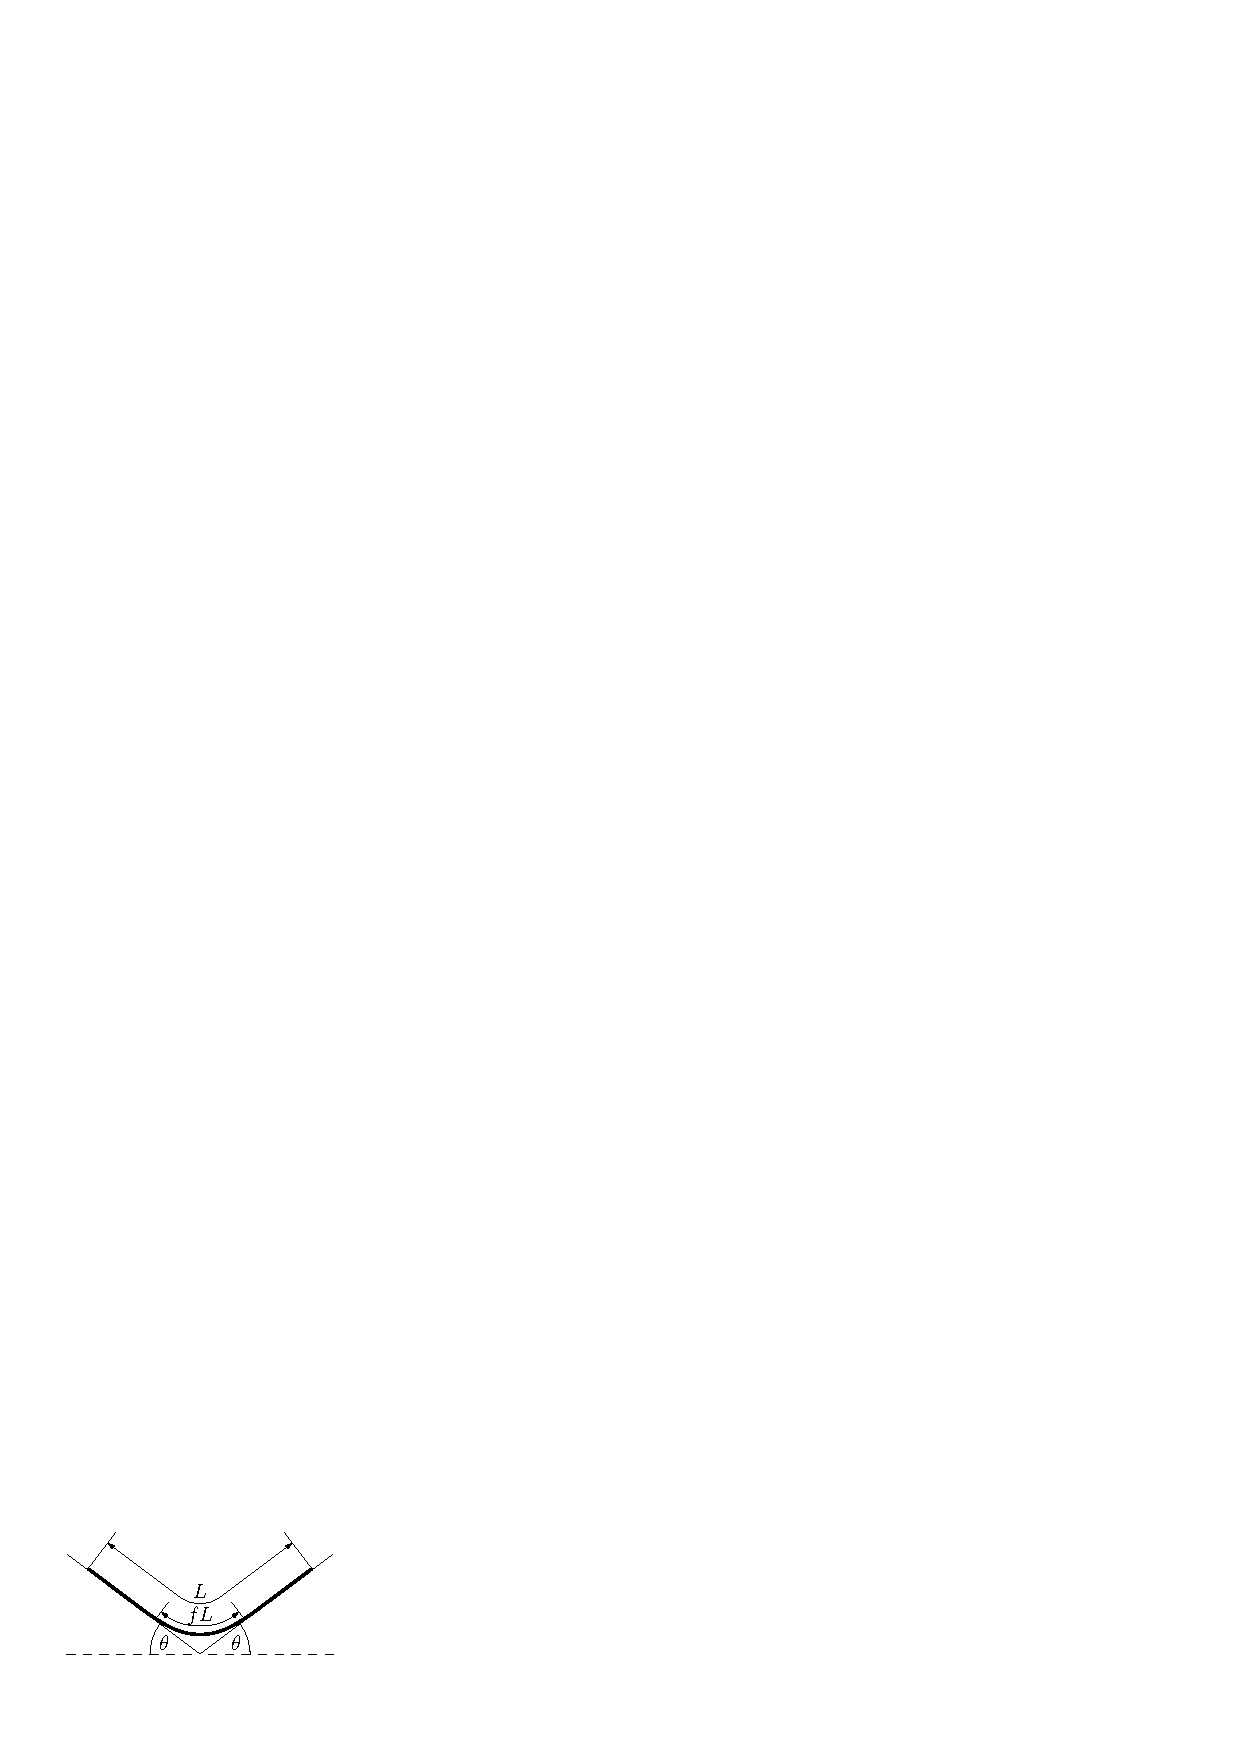
\includegraphics[width=\linewidth]{2012-lahg-09-n88r_ipe}
\end{wrapfigure}
Two plates make up a V-shaped horizontal groove. Both of the plates are at an angle $\theta$ with respect to the ground. In the groove there is a section of rope of length $L$ and of even mass distribution. All of the rope is located on the plane perpendicular to the groove so that both of the plates are touching the same amount of the rope. Above the bottom of the groove a part of the rope of length $fL$ does not anymore rest on the plates. Find $f$ if the rope is on the verge of slipping. The coefficient of friction between the rope and the plates is $\mu = 1$.
\probend
\bigskip

% P156
\setAuthor{Jaan Kalda}
\setRound{lõppvoor}
\setYear{2017}
\setNumber{G 9}
\setDifficulty{9}
\setTopic{Staatika}

\prob{Roof}
\probeng
Two stiff segments of wire with a length $L$ are connected at the ends (e.g. tied with a thread) so that their ends are at contact and the angle between them can change without resistance, making up a V-shaped figure. This system is placed on a slippery cylinder so that at the equilibrium a wire “roof” (upside down V) is formed with an apex angle $\alpha$. The mass distribution in the wire is even, there is no friction between the wire and the cylinder. a) What is the radius $R$ of the cylinder? b) What inequality should be satisfied so that this position would be stable (investigate the stability only with respect to the rotation of the “roof” as a whole, assuming that the angle between the wires does not change)?
\probend
\bigskip

% P157
\setAuthor{Jaan Kalda}
\setRound{lõppvoor}
\setYear{2015}
\setNumber{G 9}
\setDifficulty{10}
\setTopic{Staatika}

\prob{Dumbbell with a thread}
\probeng
\begin{wrapfigure}{r}{0.23\textwidth}%
\vspace{-5 pt}%
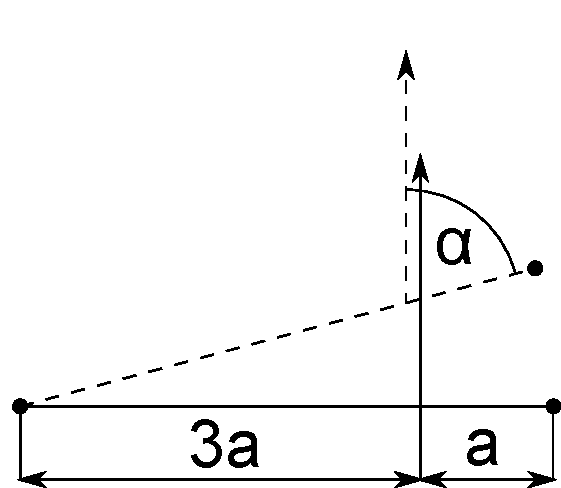
\includegraphics[width=0.23\textwidth]{2015-v3g-09-hantel}%
\vspace{-15 pt}%
\end{wrapfigure}
A dumbbell is lying on a horizontal ground. The dumbbell consists of a weightless rod of length $l=4a$ and two small blocks with identical masses and coefficients of friction that are attached to the ends of the rod. A long thread is tied to the rod at a length $a$ from one of the blocks. Initially the direction of the thread is horizontal and perpendicular to the rod. When the thread is slowly pulled the dumbbell starts to turn because at first only one block is being shifted. What is the angle $\alpha$ between the rod and the thread when the other block also starts to shift?
\probend
\bigskip
\newpage\subsection{\protect\StrSubstitute{Stellar mechanics}{-}{ }}

% P158
\setAuthor{Eero Vaher}
\setRound{piirkonnavoor}
\setYear{2014}
\setNumber{G 3}
\setDifficulty{2}
\setTopic{Taevamehaanika}

\prob{Rotation period of Earth}
\probeng
Average day, usually just called a day, is known as the average period during which the Sun seems to make a full circle in the sky for an observer located on Earth. The length of an average day is 24 h or 86 400 s. It takes Earth 365,256 average days to make one circle around the Sun. The direction of the Earth’s rotation around its axis matches the direction of its orbiting around the Sun. Using this data, find the rotation period of the Earth with the accuracy of a second.
\probend
\bigskip

% P159
\setAuthor{Mihkel Pajusalu}
\setRound{lahtine}
\setYear{2014}
\setNumber{G 3}
\setDifficulty{3}
\setTopic{Taevamehaanika}

\prob{Orbit}
\probeng
Celestial bodies revolve on elliptic orbits. The Moon’s orbit around the Earth is also elliptic. The Moon’s smallest distance from the center of mass of the Earth-Sun system (which in this problem can be assumed to coincide with the center of the Earth) is $r_{1}=\SI{360000}{km}$ and the orbital speed at that distance is $v_1=\SI{1.1}{km/s}$. Find the approximately biggest distance between the Moon and the Earth. The mass of the Earth is $M=\SI{6.0e24}{kg}$ and the gravitational constant is\\ $G=\SI{6.7e-11}{\newton\metre\squared\per\kilo\gram\squared}$.
\probend
\bigskip

% P160
\setAuthor{Eero Vaher}
\setRound{piirkonnavoor}
\setYear{2013}
\setNumber{G 6}
\setDifficulty{4}
\setTopic{Taevamehaanika}

\prob{Density of the Sun}
\probeng
Find the average density $\varrho$ of the Sun. The orbital period of the Earth is $T=1$ year, gravitational constant $G=\SI{6.7e-11}{N m^2/kg^2}$, the distance between the Earth and the Sun $R=\SI{1.5e11}{m}$, the angular diameter of the Sun observed from the Earth is $\alpha=\ang{0,54}$ (the angle that forms between the two lines that are drawn from the eye of the observer to the ends of the Sun’s diameter).
\probend
\bigskip

% P161
\setAuthor{Eero Vaher}
\setRound{piirkonnavoor}
\setYear{2018}
\setNumber{G 6}
\setDifficulty{4}
\setTopic{Taevamehaanika}

\prob{Connected satellites}
\probeng
Two satellites, both with a mass $m$, are orbiting around a planet with a mass $M\gg m$ on circular orbits of radiuses $R_1$ and $R_2=2R_1$. The satellites are connected to each other with a tensioned cable of negligible mass and of length $R_1$. Because of that the orbital period of both of the satellites is $T$. How many times are the speeds $v_1$ and $v_2$ of the satellites bigger or smaller than the speeds $v'_1$ and $v'_2$ with what the satellites would revolve on their orbits if there was no cable?
\probend
\bigskip

% P162
\setAuthor{Eero Vaher}
\setRound{lõppvoor}
\setYear{2013}
\setNumber{G 5}
\setDifficulty{5}
\setTopic{Taevamehaanika}

\prob{Satellite}
\probeng
A geostationary orbit is such an orbit that if it has a satellite on it, the satellite does not move with respect to the Earth. How big is the area of ground that can be observed from such a satellite? Give the area’s diameter measured along the surface of the Earth as an answer. The gravitational constant is $G=\SI{6.7e-11}{N \cdot m^2/kg^2}$, the Earth’s mass $M=\SI{6,0e24}{kg}$, the Earth’s radius $r=\SI{6400}{km}$, the Earth’s rotation period $t=\SI{24}{h}$.
\probend
\bigskip
\newpage\subsection{\protect\StrSubstitute{Thermodynamics}{-}{ }}

% P163
\setAuthor{Jaak Kikas}
\setRound{lahtine}
\setYear{2012}
\setNumber{G 1}
\setDifficulty{1}
\setTopic{Termodünaamika}

\prob{Freezing of water}
\probeng
\SI{0,5}{kg} of ice cubes were placed in \SI{1}{l} of water with an initial temperature \SI{0}{\degreeCelsius}. What has to be the initial temperature of the ice for the whole water to freeze? The ice’s enthalpy of fusion is \SI{330}{\kilo\joule\per\kilo\gram}, the specific heat capacity \SI{2,1}{\kilo\joule\per(\kilogram.\degreeCelsius)}. There is no heat exchange with the environment. The density of water $\rho = \SI{1000}{kg/m^3}$.
\probend
\bigskip

% P164
\setAuthor{Koit Timpmann}
\setRound{piirkonnavoor}
\setYear{2013}
\setNumber{G 2}
\setDifficulty{1}
\setTopic{Termodünaamika}

\prob{Water bottle}
\probeng
A full water bottle of volume 2,0 l was forgotten in the car during a cold weather. Coming to check his car the driver Koit could not believe his eyes: the temperature in the car was $-\SI{3}{\degreeCelsius}$ but the water in the bottle was not frozen. Koit remember he had once heard that a very clean liquid can be in liquid form even below the freezing temperature. To control this he took the bottle, shook it and in a short time some of the water turned into ice. How many grams of ice appeared in the bottle? The specific heat of water is $c = \SI{4200}{\joule\per(\kilogram \cdot \degreeCelsius)}$ and the density $\varrho = \SI{1000}{\kilogram\per\meter\cubed}$, the ice’s enthalpy of fusion $\lambda = \SI{340}{ kJ/kg}$.
\probend
\bigskip

% P165
\setAuthor{Ants Remm}
\setRound{lõppvoor}
\setYear{2012}
\setNumber{G 1}
\setDifficulty{2}
\setTopic{Termodünaamika}

\prob{Friction welding}
\probeng
A considerably new welding technology is friction welding: one of the addable details is made to rotate and pressed against the other. If the arising heat has heated the details to almost melting temperatures the rotating detail is stilled and under a big pressure a connection is formed. Let us look at a situation where one wishes to meld two copper tube segments together. Find with how much force should the tubes be pressed together during the rotation so that a big enough heat quantity would form during a time $\Delta t = \SI{6}{s}$. The tube’s speed of rotation is $f = 1200$ turns per minute. For simplification you can assume that at the ends of both of the tubes a segment of length $l
= \SI{0,5}{cm}$ is heated evenly. The diameter of the tubes is $D = \SI{8}{cm}$, the width of the wall is $d = \SI{5}{mm}$. The tubes are initially at room temperature $T_0 = \SI{20}{^\circ C}$. The connection occurs at a temperature $T_1 = \SI{810}{^\circ C}$. The copper’s coefficient of friction with itself is $\mu = 0,96$, density $\rho = \SI{8,9}{\frac{g}{cm^3}}$ and the specific heat $c = \SI{390}{\frac{J}{kg \cdot \degreeCelsius}}$. Do not account for the heat losses into the surrounding environment.
\probend
\bigskip

% P166
\setAuthor{Erkki Tempel}
\setRound{piirkonnavoor}
\setYear{2015}
\setNumber{G 3}
\setDifficulty{2}
\setTopic{Termodünaamika}

\prob{Coin in ice}
\probeng
A coin of mass $m_c=\SI{10}{g}$ and density $\rho_c=\SI{8900}{kg/m^3}$ has frozen inside a piece of ice. The temperature of the ice and the coin is $\SI{0}{\degreeCelsius}$. The piece of ice without the coin weighs $m_i=\SI{130}{g}$. This piece of ice is thrown into a vessel in where there is $V_w=\SI{400}{ml}$ of water with an initial temperature $T$. How big has to be the water’s minimal initial temperature $T$ so that the piece of ice together with the coin would sink to the bottom after the thermal equilibrium is achieved? Do not account for the heat exchange with the surrounding environment. The specific heat of water is $c=\SI{4200}{J/ (kg\cdot\degreeCelsius)}$ and the ice’s enthalpy of fusion $\lambda=\SI{330}{kJ/kg}$. The ice’s density $\rho_i=\SI{900}{kg/m^3}$ and the water’s density $\rho_w=\SI{1000}{kg/m^3}$.
\probend
\bigskip

% P167
\setAuthor{Kaur Aare Saar}
\setRound{lõppvoor}
\setYear{2016}
\setNumber{G 1}
\setDifficulty{2}
\setTopic{Termodünaamika}

\prob{Heat exchanger}
\probeng
In a backflow heat exchanger incoming oil of temperature $T_{o}=\SI{90}{\degreeCelsius}$ is cooled to a temperature $T_{0}=\SI{20}{\degreeCelsius}$. The cooling water in the heat exchanger moves to the opposite direction with respect to the oil and enters the heat exchanger with a temperature $T_{v}=\SI{10}{\degreeCelsius}$. The water moves with a speed $w_{v}=\SI{6}{\m^3\per\minute}$ and the oil with a speed $v_{o}=\SI{15}{\m^3\per\minute}$. At what temperature does the water exit the heat exchanger? The specific heat of water is $c_{w}=\SI{4200}{\joule\per\kilogram\per\degreeCelsius}$, the specific heat of oil $c_{o}=\SI{1800}{\joule\per\kilogram\per\degreeCelsius}$. The density of water $\rho_{w}=\SI{1000}{\kilogram\per\metre\cubed}$ and the density of oil $\rho_{o}=\SI{850}{\kilogram\per\metre\cubed}$.
\probend
\bigskip

% P168
\setAuthor{Oleg Košik}
\setRound{piirkonnavoor}
\setYear{2012}
\setNumber{G 2}
\setDifficulty{3}
\setTopic{Termodünaamika}

\prob{Heating system}
\probeng
Water of initial temperature $t_0=\SI{60}{\degreeCelsius}$ enters a school house’s heating system during winter. The water exits the system with a temperature $t_1=\SI{40}{\degreeCelsius}$. The power of the school house’s heat losses is $N=\SI{100}{kW}$. The diameter of the tube entering and exiting the school house is $D=\SI{100}{mm}$. Find the speed of the water in the tubes. The specific heat of water is $c=\SI{4200}{J/(kg\cdot\degreeCelsius)}$ and the density $\rho=\SI{1000}{kg/m^3}$.
\probend
\bigskip

% P169
\setAuthor{Erkki Tempel}
\setRound{lahtine}
\setYear{2015}
\setNumber{G 4}
\setDifficulty{4}
\setTopic{Termodünaamika}

\prob{Kettle}
\probeng
A kettle with a heating power $N$ is filled with water. The area of the kettle’s spout is $S$. What is the biggest speed of the water vapor exiting the kettle? Water’s enthalpy of vaporization is $L$, the universal gas constant is $R$, the air pressure is $p$ and the molar mass of water is $\mu$. The efficiency factor of the kettle without accounting for the heat losses is $\gamma$.
\probend
\bigskip

% P170
\setAuthor{Ardi Loot}
\setRound{piirkonnavoor}
\setYear{2018}
\setNumber{G 3}
\setDifficulty{4}
\setTopic{Termodünaamika}

\prob{Radiator}
\probeng
In the room there is a water radiator with a nominal power $P_{n}=\SI{2.0}{kW}$. What is the actual power of this radiator and the temperature of the water flowing back? The speed of the heating water going through the radiator is $q=\SI{1.0}{l/min}$, the temperature of the entering water is $T_{p}=\SI{70}{\degreeCelsius}$ and the room temperature is $T_{0}=\SI{22}{\degreeCelsius}$.  How big is the maximal power of the radiator for the given temperatures? The specific heat of water is $c_{w}=\SI{4200}{J/\left(kg\cdot K\right)}$ and the density $\rho_{w}=\SI{1000}{kg/m^{3}}$.\\ 
\emph{Note.} The nominal power of the radiator is its heating power for the fixed temperatures of the entering water ($T_{pn}=\SI{75}{\degreeCelsius}$), backflow water ($T_{tn}=\SI{65}{\degreeCelsius}$) and the room temperature ($T_{0n}=\SI{20}{\degreeCelsius}$).\\
\emph{Hint.} You can assume that the actual power of the radiator is proportional to the difference between the average temperature of the entering and backflow water and the room temperature.
\probend
\bigskip

% P171
\setAuthor{Kristian Kuppart}
\setRound{lahtine}
\setYear{2017}
\setNumber{G 6}
\setDifficulty{5}
\setTopic{Termodünaamika}

\prob{Greenhouse effect}
\probeng
Let us observe the following simplified model of the Earth’s atmosphere where the atmosphere layer surrounding the Earth a) reflects $\mu=\SI{30}{\%}$ of the Sun’s radiation falling on it back to the cosmos and lets the rest of the radiation through without absorbing any of it; b) absorbs completely all the infrared radiation coming from the Earth’s surface. The irradiance coming from the Sun is $w_0=\SI{1400}{\frac{W}{m^2}}$. Find the average temperature of the Earth’s surface.\\
\emph{Hint.} The Stefan-Boltzmann law applies – the power radiated by a black body per unit of area is given as $w=\sigma T^4$ where $\sigma =5,67 \cdot 10^{-8} \SI{}{\frac{W}{m^2 \cdot K^4}}$. Assume that the Earth’s surface only radiates infrared radiation and that it can be looked at as an absolutely black body due to this. The surface also absorbs all of the Sun light reaching it.
\probend
\bigskip

% P172
\setAuthor{Oleg Košik}
\setRound{lõppvoor}
\setYear{2013}
\setNumber{G 8}
\setDifficulty{7}
\setTopic{Termodünaamika}

\prob{Shop}
\probeng
Bigger buildings often have vestibules. Why? Let us take a look at a shop that was built with such a thin hall that the hall does not have an effect on the heat losses going through the walls of the shop. When opening the door of the shop a certain amount of air will go through the open door. Let us say that the air everywhere is well mixed, meaning that the outside air going into the hall through an open door has the outside temperature. We will make the same assumption for all of the doors. Let us also assume that the amount of air going through one door opening does not depend on the difference between temperatures and that the heat losses through the walls of the doors and the hall are negligible compared to the ones through the open door.\\
Let us look at the situation before the building of the hall. On a chilly April day the outside temperature during the opening hours of the shop was constantly $T_1=\SI{4}{\degreeCelsius}$. In the night, when the shop was closed, the outside temperature was a stable $T_2=\SI{0}{\degreeCelsius}$. A thermostat controls the operation of the shop’s electric radiators by holding the inner temperature steadily on $T_0=\SI{20}{\degreeCelsius}$. In the night the average power of the radiators was $P_2= \SI{5,0}{kW}$ and during the day $P_1=\SI{4,6}{kW}$. Two effects take place during the day: (a) from time to time people open the door; (b) the body warmth of the people and the lights of the shop contribute to the heating with a certain additional power.\\
After building the hall it was found out that with the same outside temperature and the number of visitors the daytime average power of the radiators decreased to $P_3=\SI{3,8}{kW}$. What power do the people and the lights in the shop produce if it is assumed that the heat exchange rate is proportional to the difference of temperatures?
\probend
\bigskip

% P173
\setAuthor{Taavi Pungas}
\setRound{piirkonnavoor}
\setYear{2014}
\setNumber{G 9}
\setDifficulty{7}
\setTopic{Termodünaamika}

\prob{Heating system}
\probeng
Let us take a look at a simplified model of an apartment building’s heating system. There is one apartment on each floor of a two story house. Let us assume that the apartments are identical. This means that the roof and the floors are well heated and we will only consider heat losses through the walls of the house.\\
In the basement there is a kettle that heats water to a temperature $t_1=\SI{68}{\degreeCelsius}$. At first the water moves to the upper apartment and there it goes through a radiator with 10 ribs. Next, the water is directed to the bottom apartment where it goes through an 11 rib radiator. After that the water moves back to the kettle and when reaching there the temperature of the water is $t_2=\SI{60}{\degreeCelsius}$. Let us assume that the water only cools in the radiators. The heating system is built so that both of the apartments have the exact same inner temperature $t$. Find the temperature $t$. \\
\emph{For your information:} heat loss through a certain wall is proportional to its area and the difference between the temperatures inside of the wall and outside. Assume that when moving through the radiator the water’s temperature decreases linearly with the distance covered.
\probend
\bigskip

% P174
\setAuthor{Andres Põldaru}
\setRound{piirkonnavoor}
\setYear{2016}
\setNumber{G 10}
\setDifficulty{7}
\setTopic{Termodünaamika}

\prob{Water heater}
\probeng
In a water heater of power $P=\SI{2.0}{kW}$ there is initially water of mass $m_0$ and of temperature $T_0=\SI{20}{\degreeCelsius}$. Additional water with a temperature $T_0$ is flowing with even speed into the heater so that the mass of the additional water per unit of time is $\mu=\const$. The heater is filled with water and the water starts to flow out of the opening on top. The temperature continues to rise, stabilizing at $\SI{36}{\degreeCelsius}$. The temperature graph of the water in the heater is shown below. Find $m_0$ and $\mu$. Assume that besides the water flowing out of the heater there are no heat losses and that the water in the heater is always with even temperature. The specific heat of water is $c=\SI{4.2}{\frac{kJ}{kg\cdot K}}$.\\
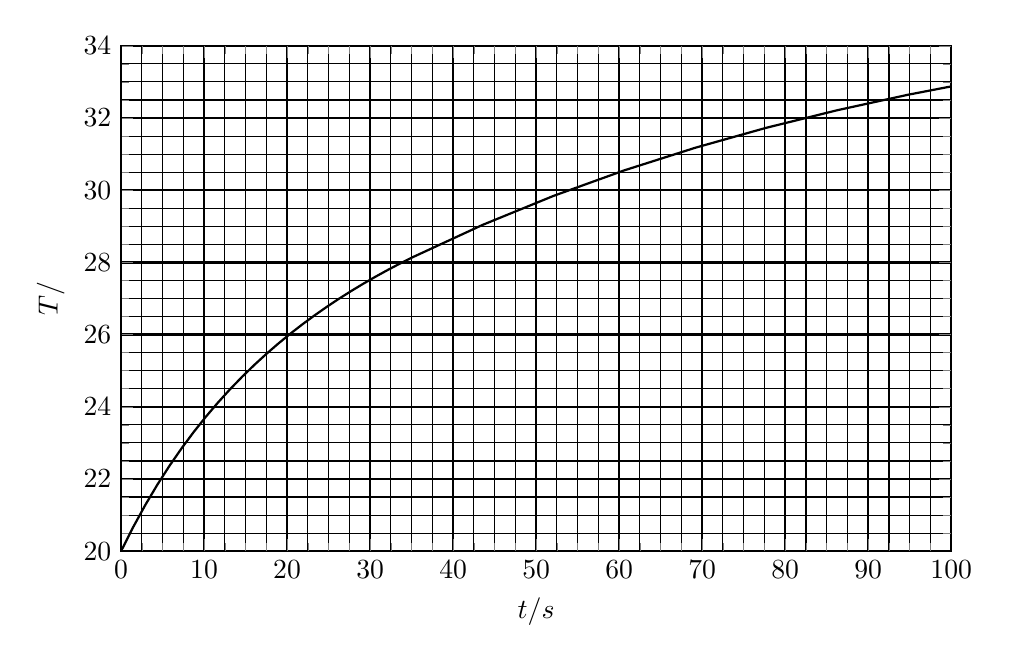
\begin{tikzpicture}
	\begin{axis}[ 
		xlabel={$t/s$},
		width = \textwidth,
		height = 8 cm,
		ylabel={$T/\si{\degreeCelsius}$},
		xmin=0, xmax = 100,
		ymin=20, ymax = 34,
		xtick distance = 10,
		ytick distance = 2,
		minor x tick num = 3,
		minor y tick num = 3,
		grid = both,
		minor grid style = {black},
		major grid style = {black, thick},
	] 
	\addplot [domain=0:35, thick]{20 + 2000/(4200*0.03)*(1-1/(1+0.03*x))};
	\addplot [domain=35:240, thick]
	{2000/(4200*0.03)+20+(20+ 2000/(4200*0.03)*(1-1/(1+0.03*35))
		-2000/(4200*0.03)-20)*e^(-0.03*(x-35)/(1+0.03*35))};
	\end{axis}
\end{tikzpicture}
\probend
\bigskip

% P175
\setAuthor{Ardi Loot}
\setRound{lõppvoor}
\setYear{2018}
\setNumber{G 5}
\setDifficulty{7}
\setTopic{Termodünaamika}

\prob{Thermal insulation}
\probeng
\begin{wrapfigure}[10]{r}{0.5\textwidth}
\vspace{-30pt}
\begin{center}
\includegraphics[width=0.5\textwidth]{2018-v3g-05-kullastunud-aur}
\par\end{center} 
\end{wrapfigure}
The insulation of a wall consists of an inner (of thermal conductivity $k_{1}=\SI{0.07}{W/\left(m\cdot K\right)}$) and an outer layer (that has a thermal conductivity $k_{2}=\SI{0.05}{W/\left(m\cdot K\right)}$). Between those layers there is a film layer to hinder the air’s movement through the wall. What condition does the width $L_{1},$ of the inner thermal insulation layer have to satisfy to avoid the condensation of water vapor in the wall? The width of the wall $L=L_{1}+L_{2}=\SI{30}{cm}$, $L_{2}$ is the width of the outer thermal insulation layer, the room temperature is $T_{1}=\SI{20}{\degreeCelsius}$, the relative humidity in the room is $\eta_{1}=\SI{60}{\percent}$ and the outside temperature $T_{2}=\SI{-20}{\degreeCelsius}$. The relation between the saturated vapor pressure of water and the temperature is shown in the figure.\\
\emph{Note.} Assume that the temperature in the insulation layer changes linearly with distance and the speed of the change is inversely proportional to thermal conductivity.
\probend
\bigskip

% P176
\setAuthor{Stanislav Zavjalov}
\setRound{lõppvoor}
\setYear{2012}
\setNumber{G 7}
\setDifficulty{8}
\setTopic{Termodünaamika}

\prob{Furnace}
\probeng
\begin{wrapfigure}{r}{0.5\textwidth}%
\includegraphics[width=\linewidth]{2012-v3g-07-ahi_graafik}%
\end{wrapfigure}
The power of a metal melting furnace’s heating element is $P_0 = \SI{50}{W}$. The furnace is turned on at room temperature and approximately after 12 minutes, when its temperature does not grow anymore, multiple preheated lead pieces with a total mass of $m = \SI{265}{g}$ are put into the oven. The relation between the temperature of the furnace and the time is shown in the figure. Based on that find the lead’s enthalpy of fusion $\lambda$.
\probend
\bigskip

% P177
\setAuthor{Ardi Loot}
\setRound{piirkonnavoor}
\setYear{2017}
\setNumber{G 10}
\setDifficulty{8}
\setTopic{Termodünaamika}

\prob{Gas heating}
\probeng
A half-spherical tent of radius $R=\SI{4}{m}$ is heated with a gas heater. The thermal conductivity of the walls is $U=\SI{3}{W/(m^{2}\cdot K)}$. $D=\SI{2.25}{}$ units of mass of water segregates when burning one unit of mass of gas. The calorific value of the gas is $k=\SI{40}{MJ/kg}$. The temperature of the outside air is $T_{0}=\SI{-10}{\degreeCelsius}$ and the humidity $\eta_{0}=\SI{50}{\percent}$. How big has to be the gas heater’s power $P$ and the tent’s ventilation air volume $Q$ per unit of time so that the temperature in the tent would be at $T_{1}=\SI{15}{\degreeCelsius}$ and the humidity $\eta_{1}=\SI{80}{\percent}$? How big part of the heating power goes to the heating of the ventilation air and how many times per hour does the air in the tent change?\\
The air density is $\rho_{a}=\SI{1.2}{kg/m^{3}}$ and the heat capacity $c_{a}=\SI{1.0}{kJ/(kg\cdot K)}$. At the temperature $T_{0}=\SI{-10}{\degreeCelsius}$ maximally $G_{0}=\SI{2.3}{g/m^{3}}$ of water vapor can fit into a unit of volume of air and at the temperature $T_{1}=\SI{15}{\degreeCelsius}$ accordingly $G_{1}=\SI{12.8}{g/m^{3}}$. Assume that there are no heat losses through the floor of the tent.
\probend
\bigskip

% P178
\setAuthor{Mihkel Pajusalu}
\setRound{lahtine}
\setYear{2014}
\setNumber{G 9}
\setDifficulty{9}
\setTopic{Termodünaamika}

\prob{Black cube}
\probeng
Let there be an absolutely black cube made of a material with very good heat conductivity. The cube is placed in front of a parallel light beam with an intensity (power per cross section area) $I$. What is the maximal and minimal stable temperature $T_\text{max}$ and $T_\text{min}$ that the cube attains depending on its position with respect to the direction of the radiation’s spreading?
\probend
\bigskip
\newpage\subsection{\protect\StrSubstitute{Miscellaneous}{-}{ }}

% P179
\setAuthor{EFO žürii}
\setRound{piirkonnavoor}
\setYear{2018}
\setNumber{G 1}
\setDifficulty{1}
\setTopic{Varia}

\prob{Contraction}
\probeng
$V_w$ liters of water and $V_e$ liters of ethanol are mixed with each other so that the volume of their solution is $V=\SI{1}{dm^3}$ and that by mass there is $p=\SI{44,1}{\percent}$ of ethanol in the solution. Find the volumes $V_w$ and $V_e$ of the water and ethanol mixed with each other. When pouring the solutions together there is a $\gamma = \SI{6}{\percent}$ of contraction – the volume of the acquired solution is 6\% smaller than the total volume of water and ethanol. The density of water is $\rho_w=\SI{1000}{kg/m^3}$ and ethanol $\rho_e=\SI{790}{kg/m^3}$.
\probend
\bigskip

% P180
\setAuthor{Mihkel Kree}
\setRound{piirkonnavoor}
\setYear{2014}
\setNumber{G 4}
\setDifficulty{3}
\setTopic{Varia}

\prob{Mobile charger}
\probeng
Inventors have come up with a device for hikers to charge their telephone. A mechanism that works as a shock absorber is put inside the sole of one boot. Every time a person leans on the sole the mechanical work is transformed into electrical energy with the help of a little electric generator. Let us assume that the mass of the hiker is $m=\SI{60}{kg}$ and that during one step her sole sinks by $h=\SI{5}{mm}$. The efficiency of this device is $\eta = \SI{0,2}{}$. The average length of the hiker’s pair of steps, meaning the distance between two consecutive steps on the same sole is $d=\SI{1.5}{m}$. Now the telephone needs to be connected to the sole with a cord and the charging may begin.\\
Take into account that in a typical smart phone there is a lithium polymer battery that works on a voltage $U=\SI{3.7}{V}$. Also assume that if the telephone works on an average current strength $I_a=\SI{130}{mA}$ the battery would withstand for $T=10$. Calculate what distance does the hiker have to walk to charge an empty telephone battery full again.
\probend
\bigskip

% P181
\setAuthor{Valter Kiisk}
\setRound{lõppvoor}
\setYear{2017}
\setNumber{G 3}
\setDifficulty{3}
\setTopic{Varia}

\prob{Laser}
\probeng
A laser beam with an even diameter $d=\SI{1}{mm}$ falls perpendicularly to the first surface of a wedge-shaped glass plate (the angle between the surfaces $\varphi=\ang{2}$). The laser beam consists of monochromatic components with wavelengths $\lambda_1=\SI{355}{nm}$ and $\lambda_2=\SI{532}{nm}$. The refractive indexes of the glass on these wavelengths are accordingly $n_1=\num{1.48}$ and $n_2=\num{1.46}$. Find the distance $l$ between the glass plate and the location where the light beams with different wavelength are completely separated from each other.
\probend
\bigskip

% P182
\setAuthor{Koit Timpmann}
\setRound{lahtine}
\setYear{2011}
\setNumber{G 2}
\setDifficulty{4}
\setTopic{Varia}

\prob{Surface tension}
\probeng
A glass tube (radius $r_1$) is placed inside a thicker glass tube so that their axes coincide. Next they are both placed upright in water. Find how big should be the inner radius $r_2$ of the thicker tube so that the water level inside both of the glass tubes would be the same. Assume that the walls of the tubes are insignificantly thin.
\probend
\bigskip

% P183
\setAuthor{Ants Remm}
\setRound{lahtine}
\setYear{2011}
\setNumber{G 4}
\setDifficulty{4}
\setTopic{Varia}

\prob{Smurf in solarium}
\probeng
Smurf spent $t = \SI{10}{min} $ under the lights of a solarium. What heat $ Q $ did Smurf receive? The incident light spectrum $I$ of Smurf (intensity per wavelength depending on the wavelength of the light, unit \SI{10e9}{W/m^3}) and the absorbed spectrum $\varepsilon$ of Smurf (the relation between the absorbed and incident intensity as a function of wavelength) are given in the figure. The effective area where the light falls on Smurf is $ S = \SI{0,1}{m^2} $.

\begin{center}
\includegraphics[width=0.49\textwidth]{2011-lahg-04-I}
\includegraphics[width=0.49\textwidth]{2011-lahg-04-epsilon}
\end{center}
\probend
\bigskip

% P184
\setAuthor{Valter Kiisk}
\setRound{piirkonnavoor}
\setYear{2016}
\setNumber{G 7}
\setDifficulty{4}
\setTopic{Varia}

\prob{Lights}
\probeng
At a distance $l_1=\SI{15}{cm}$ from a luminescence tube the illuminance was measured to be $L_1=\SI{8400}{lx}$. The luminescence tube can be assumed to be much longer than the distance $l_1$. However, at a distance $l_2=\SI{30}{cm}$ from a LED bulb the illuminance was measured to be $L_2=\SI{2600}{lx}$. Luminescence tubes in an office room are placed on a straight row over the whole room at a height $h_1=\SI{1.8}{m}$ from the working plane. A desk lamp’s LED bulb is located at a height $h_2=\SI{40}{cm}$ from the table’s surface. How big illuminance is achieved directly below the light separately in the case of general lighting and spot lighting?\\
\emph{Note.} illuminance characterizes the light energy falling on a unit of area per unit of time.
\probend
\bigskip

% P185
\setAuthor{Taavi Pungas}
\setRound{lõppvoor}
\setYear{2013}
\setNumber{G 6}
\setDifficulty{5}
\setTopic{Varia}

\prob{Pond}
\probeng
\begin{wrapfigure}{r}{0.25\textwidth}%
\includegraphics[width=\linewidth]{2013-v3g-06-lained}%
\end{wrapfigure}
Let us take a look at the waves forming around a stone thrown into a pond. When the stone falls into the water a big amount of disturbances with different wavelengths form, each of them propagating with their own speed. When they are merged a wave crest is formed and we can observe the crest’s movement. The locations of this crest, each of them after a specific amount of time, are shown in the figure, the scale is a straight line of length $L$. The speed $v$ of the crest depends on the wavelengths $\lambda$ of the components it is currently made of and on the depth $h$ of the water. If a time $t$ that has passed from throwing the stone into the water is small then the crest consists of wavelengths $\lambda \ll h$ and the speed of the wavelength depends on the time as $v \approx \frac{gt}{\pi}$. Further, where the disturbances that create a crest have a wavelength $\lambda \gg h$, the wavelength moves with a speed $v
\approx \sqrt{hg}$. Evaluate the depth $h$ assuming that it is the same over the whole pond. Give the answer as a ratio of $h/L$.
\probend
\bigskip

% P186
\setAuthor{Mihkel Kree}
\setRound{lõppvoor}
\setYear{2016}
\setNumber{G 5}
\setDifficulty{5}
\setTopic{Varia}

\prob{Radon}
\probeng
Graptolitic argillite (also known as dictyonema shale) is a sedimentary claystone found in North-Estonia that consists of numerous rare elements, such as uranium. One ton of the rock contains 300 g of uranium-238 isotope. It is the most common uranium isotope, its atomic mass is $238$, half-life $\tau\idx{U}=\SI{4.5}{}$ billion years and a intermediate element of its decay chain is radioactive radon with an atomic mass $222$ and half-life $\tau\idx{Rn}=\SI{3.8}{}$ days. Radon is a gas that is believed to cause lung cancer because when breathing it in its radioactive decay products get into the organism. Because of this established norms require that the activity of radon in the room air of buildings has to be smaller than $\SI{200}{Bq/m^3}$, where the unit Bq named after Henri Becquerel stands for the decay of one nucleus per second.\\
A hiker unknowingly brought home a piece of graptolitic argillite of mass $m$ and placed it on the shelf of a bedroom. Assume that there is no air exchange in the bedroom which has a volume $V=\SI{25}{m^3}$ and that all of the gaseous radon leaves the rock. Assuming that the rock is held in the room for a long time, find the biggest harmless mass $m$ of the rock so that the radon activity caused by it still stays within the norms.\\
\emph{Note.} atomic mass unit $u=\SI{1.7e-27}{kg}$.
\probend
\bigskip

% P187
\setAuthor{Jaan Kalda}
\setRound{piirkonnavoor}
\setYear{2012}
\setNumber{G 7}
\setDifficulty{7}
\setTopic{Varia}

\prob{Rain}
\probeng
A house has a mirror symmetric gable roof: the vertical plane of symmetry is East-West directional and the North and South sides of the roof are perpendicular to each other. At both sides of the roof there is a rainwater gutter that collects the water falling on the roof and directs it into a barrel. It is raining and South wind is blowing $u= \SI{6,0}{m/s}$. The barrel at the South side fills 2,0 times faster than the barrel at the North side. You can assume that the direction of the falling rain drops does not change significantly. What is the average speed of the falling drops (meaning the velocity’s vertical component)?
\probend
\bigskip

% P188
\setAuthor{Jaan Kalda}
\setRound{lõppvoor}
\setYear{2015}
\setNumber{G 6}
\setDifficulty{8}
\setTopic{Varia}

\prob{Shock wave}
\probeng
An electrostatic shock wave that travels with a speed $w$ along the $x$-axis can be described by an electric potential: $U=0$ if $x<wt$ and $U=U_0$ if $x>wt$. What speed $v$ does an initially still particle of mass $m$ and charge $q$ obtain under a shock wave? The answer should depend on the height $U_0$ of the potential barrier. Keep in mind that whether the particle stays on one side of the barrier or the other depends on the value of $U_0$.
\probend
\bigskip

% P189
\setAuthor{Jaan Kalda}
\setRound{lahtine}
\setYear{2013}
\setNumber{G 10}
\setDifficulty{10}
\setTopic{Varia}

\prob{Shadow of a balloon}
\probeng
A spherical opaque balloon is floating during a sunny day and leaves a shadow on a horizontal ground, moreover the length of the penumbra is 5.0 m and the width 2.5 m and the length of the umbra is 1.0 m. How big is the diameter of the ball and how high is it from the ground? The apparent angular diameter of the Sun (the angle that forms between the two lines that are drawn from the eye of the observer to the ends of the Sun’s diameter) was $\alpha =0.53^\circ$ during that day.
\probend
\bigskip
\newpage\subsection{\protect\StrSubstitute{Liquid mechanics}{-}{ }}

% P190
\setAuthor{Koit Timpmann}
\setRound{piirkonnavoor}
\setYear{2012}
\setNumber{G 3}
\setDifficulty{2}
\setTopic{Vedelike mehaanika}

\prob{Barrel}
\probeng
An empty barrel floating in water has $1/10$ of its volume inside water. After filling the barrel with an unknown liquid the barrel will stay floating on the water but now $9/10$ of the barrel’s volume is inside the water. What is the density of the liquid that the barrel is filled with? The density of water is $\SI{1000}{kg/m^3}$.
\probend
\bigskip

% P191
\setAuthor{Hans Daniel Kaimre}
\setRound{lõppvoor}
\setYear{2018}
\setNumber{G 2}
\setDifficulty{3}
\setTopic{Vedelike mehaanika}

\prob{Hole in a barrel}
\probeng
A big barrel filled with water has a hole in the bottom and the water is flowing out of it. The ratio between the diameter of the exiting water flow and the distance $l$ from the bottom of the barrel is shown in the figure. Find the height of the water level inside the barrel.
\begin{center}
\includegraphics[width = 0.6\linewidth]{2018-v3g-02-juga_ing}
\end{center}
\probend
\bigskip

% P192
\setAuthor{Koit Timpmann}
\setRound{lõppvoor}
\setYear{2015}
\setNumber{G 3}
\setDifficulty{4}
\setTopic{Vedelike mehaanika}

\prob{Floating cube}
\probeng
A thin-walled hermetic cube is floating on the surface of a liquid. The density of the liquid is $\rho$, the mass of the cube with the gas inside it is $m$ and its edge length is $a$. What is the smallest initial pressure $p$ of the gas in the cube so that the cube would not drown if a hole would be made in its bottom? The air pressure is $p_0$, gravitational acceleration is $g$.
\probend
\bigskip

% P193
\setAuthor{Ardi Loot}
\setRound{piirkonnavoor}
\setYear{2018}
\setNumber{G 4}
\setDifficulty{4}
\setTopic{Vedelike mehaanika}

\prob{Pump}
\probeng
One wants to pump water out from a well with a depth $h=\SI{5.0}{m}$. The pump is on the surface and its water intake pipe (filled with water) has an inner diameter $d=\SI{16}{mm}$ and a length that is equal to the depth of the well.\\
a) How big has to be the power $P$ of the pump to pump water with a flow rate $q=\SI{30}{l/min}$? The efficiency of the pump is $\eta=\SI{25}{\percent}$.\\
b) What is the maximal depth $h_{m}$ of the well for which it is possible to pump water from the well with this type of pump?\\
Assume that besides other forces frictional force is also applied to the water column inside the water, which causes a decrease in the pressure per length $l$ of the pipe $\Delta p=c_{h}q^{2}l/d^{5}$ where $c_{h}=\SI{40}{Pa\cdot s^{2}/m^{2}}$. The density of water $\rho=\SI{1000}{kg/m^{3}}$, gravitational acceleration $g=\SI{9.8}{m/s^{2}}$ and the air pressure $p_{0}=\SI{100}{kPa}$.
\probend
\bigskip

% P194
\setAuthor{Siim Ainsaar}
\setRound{piirkonnavoor}
\setYear{2013}
\setNumber{G 7}
\setDifficulty{5}
\setTopic{Vedelike mehaanika}

\prob{Glass of water}
\probeng
Water was poured into a cylindrical glass to a height $H$. The height of the glass itself was $h$ and its radius $r$. The glass was covered with a sheet of paper and turned upside down; the volume of the water that flowed out between the paper and glass was $V$. When the paper was no longer held against the glass it still stayed attached to it, the rest of the water stayed in the glass. What was the maximal mass $m$ of the paper? The air pressure was $p_0$, gravitational acceleration $g$ and density of water $\varrho$. Coated paper was used and it did not absorb water. In the moment of releasing the paper the temperatures of the air and water were equal.
\probend
\bigskip

% P195
\setAuthor{Erkki Tempel}
\setRound{lahtine}
\setYear{2014}
\setNumber{G 6}
\setDifficulty{5}
\setTopic{Vedelike mehaanika}

\prob{Block in liquids}
\probeng
In a cylindrical vessel with a bottom area $S$ there are two non-miscible liquids with densities $\rho_1$ and $\rho_2$. A cube-shaped block of volume $V$ and density $\rho_k$ ($\rho_1>\rho_k>\rho_2$) is placed inside the vessel. The block is completely inside the liquids and does not touch the bottom of the vessel.\\
\osa How big part of the block is located in the bottom liquid?\\
\osa How much does the height of the separating surface of the two liquids change after placing the block inside the vessel?
\probend
\bigskip

% P196
\setAuthor{Jonatan Kalmus}
\setRound{piirkonnavoor}
\setYear{2018}
\setNumber{G 7}
\setDifficulty{5}
\setTopic{Vedelike mehaanika}

\prob{Cube with water}
\probeng
Find the mass of the water that has to be poured into a cube so that the cube would be as stable as possible, meaning that the system’s center of mass would be as low as possible. The length of the cube’s edge is $a$, the mass $M$, density of water $\rho$. Do not consider the width of the cube’s wall. The cube is completely symmetrical meaning that it has all 6 identical faces.
\probend
\bigskip

% P197
\setAuthor{Mihkel Heidelberg}
\setRound{lahtine}
\setYear{2012}
\setNumber{G 5}
\setDifficulty{6}
\setTopic{Vedelike mehaanika}

\prob{Submarine}
\probeng
\begin{wrapfigure}{r}{0.51\linewidth}%
\includegraphics[width=\linewidth]{2012-lahg-05-allveelaev_g_ing}%
\end{wrapfigure}
Secret agent Bond is escaping from a submarine through its tower. Initially the pressure in the tower is the same as the air pressure on the water: $p_0 = \SI{100}{kPa}$. After closing the hatch that separates the tower from the rest of the submarine Bond makes a hole inside the tower’s wall (see figure), after which the tower partly fills with water. Next, Bond opens the ceiling hatch and swims to the surface with the released air.\\
a) How thick is the air layer that is inside the tower before opening the ceiling hatch and after the water has stopped flowing inside?\\
b) How big and to what direction (up or down) is the total force applied to the ceiling hatch by the air and the water before opening the hatch and during the time when the water level inside tower has stilled?\\
The area of the hatch is $S =
\SI{0,50}{m^2}$, the water level above the hatch $h=\SI{25}{m}$, the height of the tower $s=\SI{2,0}{m}$. The density of water $\rho = \SI{1000}{kg/m^3}$, gravitational acceleration $g =
\SI{9,8}{m/s^2}$.
\probend
\bigskip

% P198
\setAuthor{Taavi Pungas}
\setRound{lahtine}
\setYear{2013}
\setNumber{G 7}
\setDifficulty{7}
\setTopic{Vedelike mehaanika}

\prob{Bowl}
\probeng
A cylindrical metal bowl of mass $M=\SI{1}{kg}$ and volume $V_1=\SI{3}{dm^3}$ is floating in a tube. Mari makes an experiment - during a time period $t=\SI{1}{s}$ she pours evenly a jug full of water with a volume $V_2=\SI{1,5}{dm^3}$ into the bowl from a height $h=\SI{1,5}{m}$. Predict the result of the experiment: does the bowl go to the bottom or not? Explain your prediction with calculations. The density of water $\rho=\SI{1000}{kg/m^3}$.
\probend
\bigskip

% P199
\setAuthor{Mihkel Kree}
\setRound{lahtine}
\setYear{2015}
\setNumber{G 7}
\setDifficulty{7}
\setTopic{Vedelike mehaanika}

\prob{Water spurts}
\probeng
\begin{wrapfigure}{r}{0.2\textwidth}%
\vspace{-15pt}
\includegraphics[width=\linewidth]{2015-lahg-07-veejoadJoon}%
\end{wrapfigure}
Small holes at numerous different heights have been made into the wall of a vertical cylindrical vessel and water is flowing out of them. Additional water is slowly poured into the vessel so that the water level inside the vessel is constantly at a height $H$. Find what region of room can the exiting water reach, in other words express the equation for the envelope of the water spurts in $xy$-coordinates. Assume that different water spurts do not affect each other.
\probend
\bigskip

% P200
\setAuthor{Erkki Tempel}
\setRound{piirkonnavoor}
\setYear{2016}
\setNumber{G 9}
\setDifficulty{7}
\setTopic{Vedelike mehaanika}

\prob{U-tube}
\probeng
Water of density $\rho_w$ has been poured inside a U-tube with an even cross-sectional area S so that over half of the U-tube is filled with the water and the length of each of the unfilled part is $h$. One end of the U-tube is closed hermetically and into the other end oil is slowly poured up to the edge. How big was the density $\rho_{o}$ of the oil if it is known that the height of the added oil column was $l$? The atmosphere pressure is $p_0$.
\probend
\bigskip
\newpage\normalsize\section{Hints}
        \toggleHint
        
% H1
\setAuthor{Erkki Tempel}
\setRound{piirkonnavoor}
\setYear{2014}
\setNumber{G 1}
\setDifficulty{1}
\setTopic{Dünaamika}

\prob{Flying bottle}
\hinteng
The exact same forces apply for both the bottle and the water, they are also thrown with the same initial speed.
\probend
\bigskip

% H2
\setAuthor{Erkki Tempel}
\setRound{piirkonnavoor}
\setYear{2014}
\setNumber{G 2}
\setDifficulty{1}
\setTopic{Dünaamika}

\prob{Cheburashka and nuts}
\hinteng
This situation is easier to study at the train’s frame of reference.
\probend
\bigskip

% H3
\setAuthor{Mihkel Rähn}
\setRound{lahtine}
\setYear{2016}
\setNumber{G 2}
\setDifficulty{1}
\setTopic{Dünaamika}

\prob{Curve}
\hinteng
The passengers of the car do not feel a sideways force when the total force is perpendicular to the road’s surface.
\probend
\bigskip

% H4
\setAuthor{Eero Vaher}
\setRound{lahtine}
\setYear{2012}
\setNumber{G 2}
\setDifficulty{2}
\setTopic{Dünaamika}

\prob{Lost wallet}
\hinteng
At the bottom section of the jumping track the wallet has obtained a certain horizontal speed. After that the wallet starts to move along a parabolic trajectory until it falls against the mountain’s surface again.
\probend
\bigskip

% H5
\setAuthor{Taavi Pungas}
\setRound{lahtine}
\setYear{2013}
\setNumber{G 1}
\setDifficulty{2}
\setTopic{Dünaamika}

\prob{Rock}
\hinteng
The match starts to slide down the hemisphere when the component of the gravity force that is parallel to the surface exceeds the friction force.
\probend
\bigskip

% H6
\setAuthor{Taavi Pungas}
\setRound{piirkonnavoor}
\setYear{2013}
\setNumber{G 4}
\setDifficulty{2}
\setTopic{Dünaamika}

\prob{Sledge}
\hinteng
For fixed $h$ and $t$ the slope’s inclination is smallest when there is no friction force
\probend
\bigskip

% H7
\setAuthor{Taivo Pungas}
\setRound{lõppvoor}
\setYear{2013}
\setNumber{G 2}
\setDifficulty{2}
\setTopic{Dünaamika}

\prob{Ball}
\hinteng
The height of the ball’s flight depends on the squared time it takes to reach this height.
\probend
\bigskip

% H8
\setAuthor{Mihkel Rähn}
\setRound{lahtine}
\setYear{2014}
\setNumber{G 1}
\setDifficulty{2}
\setTopic{Dünaamika}

\prob{Freight train}
\hinteng
a) On a horizontal road the freight train has to overcome the hindering friction force.\\
b) In addition to the friction force the train now also has to overcome the gravity force.
\probend
\bigskip

% H9
\setAuthor{Andreas Valdmann}
\setRound{lahtine}
\setYear{2014}
\setNumber{G 2}
\setDifficulty{2}
\setTopic{Dünaamika}

\prob{Vacuum cannon}
\hinteng
The ball divides the cannon tube into two chambers. After rupturing the left membrane the gas in the left chamber starts to press the ball to the right side.
\probend
\bigskip

% H10
\setAuthor{EFO žürii}
\setRound{lahtine}
\setYear{2016}
\setNumber{G 1}
\setDifficulty{2}
\setTopic{Dünaamika}

\prob{Toy cannon}
\hinteng
Because the ball lands perpendicularly to the inclined surface then at this moment the ball moves at the angle $\alpha$ with respect to the vertical. Thus the ball is fired out of the cannon also at the angle $\alpha$ with respect to the vertical and then the ball bounces back from the inclined surface at the same angle.
\probend
\bigskip

% H11
\setAuthor{Oleg Košik}
\setRound{piirkonnavoor}
\setYear{2016}
\setNumber{G 2}
\setDifficulty{2}
\setTopic{Dünaamika}

\prob{Tug of war}
\hinteng
According to the Newton’s third law the pulling force for both of the men is the same, but at opposite directions. In addition to the rope’s pull a friction force at opposite directions applies for both of the men.
\probend
\bigskip

% H12
\setAuthor{Moorits Mihkel Muru}
\setRound{lõppvoor}
\setYear{2017}
\setNumber{G 1}
\setDifficulty{2}
\setTopic{Dünaamika}

\prob{Fastelavn slide}
\hinteng
The energy spent due to the friction force depends on the distance covered and its inclination, the difference of the potential energy depends on the change of height.
\probend
\bigskip

% H13
\setAuthor{Kaur Aare Saar}
\setRound{lahtine}
\setYear{2013}
\setNumber{G 3}
\setDifficulty{3}
\setTopic{Dünaamika}

\prob{Alpinist}
\hinteng
Reaching the lowest point of the fall, the potential energy of the alpinist has transformed into the spring’s potential energy. Writing down the according relation, it is possible to find the rope’s extension $x$.
\probend
\bigskip

% H14
\setAuthor{Taavi Pungas}
\setRound{piirkonnavoor}
\setYear{2014}
\setNumber{G 5}
\setDifficulty{3}
\setTopic{Dünaamika}

\prob{Parachute jump}
\hinteng
The friction force of the air with a same coefficient applies for both Juku and Juhan, that force is completely balanced by the gravity force.
\probend
\bigskip

% H15
\setAuthor{Joonas Kalda}
\setRound{piirkonnavoor}
\setYear{2016}
\setNumber{G 4}
\setDifficulty{3}
\setTopic{Dünaamika}

\prob{Sledge}
\hinteng
At a limit case Juku’s total potential energy goes to the heat energy caused by the friction force.
\probend
\bigskip

% H16
\setAuthor{Eero Vaher}
\setRound{lõppvoor}
\setYear{2016}
\setNumber{G 2}
\setDifficulty{3}
\setTopic{Dünaamika}

\prob{Car’s braking}
\hinteng
The car’s kinetic energy goes to overcoming the braking force and bringing the change in potential energy.
\probend
\bigskip

% H17
\setAuthor{Hans Daniel Kaimre}
\setRound{lõppvoor}
\setYear{2016}
\setNumber{G 3}
\setDifficulty{3}
\setTopic{Dünaamika}

\prob{Cannonball}
\hinteng
To find the actual height of the ball from the Earth’s ground, you can use the law of conservation of energy at the moment of shooting the ball and at the highest point of the trajectory.
\probend
\bigskip

% H18
\setAuthor{Andreas Valdmann}
\setRound{piirkonnavoor}
\setYear{2017}
\setNumber{G 3}
\setDifficulty{3}
\setTopic{Dünaamika}

\prob{Pendulum}
\hinteng
Three forces apply to the weight: the thread’s tension, gravitational acceleration and the centripetal acceleration. In addition, the resultant force has to be perpendicular to the string because otherwise the string must extend or shorten when the weights accelerates.
\probend
\bigskip

% H19
\setAuthor{Jonatan Kalmus}
\setRound{lõppvoor}
\setYear{2017}
\setNumber{G 2}
\setDifficulty{3}
\setTopic{Dünaamika}

\prob{Mountain’s slope}
\hinteng
During a half of the pedal turn the work done by the cyclist has to compensate for the change in potential energy caused by the rise of the bicycle’s center of mass.
\probend
\bigskip

% H20
\setAuthor{Kristian Kuppart}
\setRound{lahtine}
\setYear{2011}
\setNumber{G 3}
\setDifficulty{4}
\setTopic{Dünaamika}

\prob{Truck}
\hinteng
The water surface takes a position that is perpendicular to the resultant force applied to it. Moving to the frame of reference of the truck we can see that the resultant acceleration of the truck is $\vec g - \vec a$.
\probend
\bigskip

% H21
\setAuthor{Andreas Valdmann}
\setRound{piirkonnavoor}
\setYear{2012}
\setNumber{G 5}
\setDifficulty{4}
\setTopic{Dünaamika}

\prob{Loop-the-loop track}
\hinteng
Gravity force and normal force are applied to the car. To stay in the loop the normal reaction must not disappear. The critical situation is at the upper point of the loop because then the car’s speed is the smallest and the gravity force pulls the car maximally away from the road.
\probend
\bigskip

% H22
\setAuthor{Mihkel Kree}
\setRound{lõppvoor}
\setYear{2012}
\setNumber{G 2}
\setDifficulty{4}
\setTopic{Dünaamika}

\prob{Water spurt}
\hinteng
The water exiting the tube moves like a free falling body with a horizontally directed initial speed $v$. Thus, the water spurt is shaped like a parabola, the parameters of it can be measured in the figure.
\probend
\bigskip

% H23
\setAuthor{Aigar Vaigu}
\setRound{piirkonnavoor}
\setYear{2016}
\setNumber{G 6}
\setDifficulty{4}
\setTopic{Dünaamika}

\prob{Shooting range}
\hinteng
The ball is moving along a parabolic trajectory, moreover the horizontal component of the velocity stays constant, meaning $v_x = \const = v\cos\alpha$ and the vertical component is evenly accelerating $v_y = v\sin\alpha - gt$.
\probend
\bigskip

% H24
\setAuthor{Kaur Aare Saar}
\setRound{lõppvoor}
\setYear{2016}
\setNumber{G 4}
\setDifficulty{4}
\setTopic{Dünaamika}

\prob{Cylinder}
\hinteng
The angular momentum of the cylinder does not change with respect to the axis that goes through the contact points of the cylinder and the plane because the friction force is missing the respective torque arm.
\probend
\bigskip

% H25
\setAuthor{Jonatan Kalmus}
\setRound{piirkonnavoor}
\setYear{2018}
\setNumber{G 5}
\setDifficulty{4}
\setTopic{Dünaamika}

\prob{Truck on a roundabout}
\hinteng
If the speed gets too big, due to centrifugal force the truck will start to turn around with respect to the edge of the outer curve. Thus in the limit case torque balance must apply to this axis.
\probend
\bigskip

% H26
\setAuthor{Ants Remm}
\setRound{lahtine}
\setYear{2012}
\setNumber{G 6}
\setDifficulty{5}
\setTopic{Dünaamika}

\prob{Chlorine’s molecule}
\hinteng
During the division the total momentum and energy must remain. The velocities of the particles are easier to observe by components. For that you can assume that the $x$-axis is parallel to the initial direction of the molecule and the $y$-axis perpendicular to it.
\probend
\bigskip

% H27
\setAuthor{Andres Põldaru}
\setRound{lahtine}
\setYear{2014}
\setNumber{G 5}
\setDifficulty{5}
\setTopic{Dünaamika}

\prob{Swing}
\hinteng
During the collision principle of moments applies for both of the masses. Additionally, the collision will last until the masses rotate around the swing with the same angular velocities.
\probend
\bigskip

% H28
\setAuthor{Jaan Toots}
\setRound{lahtine}
\setYear{2015}
\setNumber{G 6}
\setDifficulty{5}
\setTopic{Dünaamika}

\prob{Hydrogen’s ionization}
\hinteng
To ionize the hydrogen atom the electron’s kinetic energy must be bigger than $E_0$. During the collision of the electron and the proton both the total kinetic energy and the total momentum is preserved.
\probend
\bigskip

% H29
\setAuthor{Kristian Kuppart}
\setRound{piirkonnavoor}
\setYear{2015}
\setNumber{G 5}
\setDifficulty{5}
\setTopic{Dünaamika}

\prob{Water pipe}
\hinteng
The sharply turning water at the end of the pipe presses the pipe sideways with a certain force. This force can be found when you observe the momentum change of the exiting water per unit of time compared to the entering water.
\probend
\bigskip

% H30
\setAuthor{Mihkel Kree}
\setRound{piirkonnavoor}
\setYear{2015}
\setNumber{G 6}
\setDifficulty{5}
\setTopic{Dünaamika}

\prob{Collision}
\hinteng
Because the collision is elastic the kinetic energy will be preserved during the collision. You cannot say the same for momentum because forces are applied to the attachment points during the collision. However, the total angular momentum with respect to the attachment point is preserved in the system because during the collision the torque arms applied to the attachment point are zero and the collision happens so fast that you do not have to consider the gravity force.
\probend
\bigskip

% H31
\setAuthor{Ardi Loot}
\setRound{lahtine}
\setYear{2016}
\setNumber{G 6}
\setDifficulty{5}
\setTopic{Dünaamika}

\prob{Cyclist}
\hinteng
During the descent three forces are applied to the cyclist: the gravity force helping the descent, hindering friction force and the air resistance. The cyclist has achieved the final speed when these forces have balanced.
\probend
\bigskip

% H32
\setAuthor{Rasmus Kisel}
\setRound{piirkonnavoor}
\setYear{2017}
\setNumber{G 7}
\setDifficulty{5}
\setTopic{Dünaamika}

\prob{Two balls and a spring}
\hinteng
Even though the mass of the unknown ball and the stiffness of the spring are not known, they can still be treated as unknown values and hope that they cancel out in the final answer.
\probend
\bigskip

% H33
\setAuthor{Moorits Mihkel Muru}
\setRound{lõppvoor}
\setYear{2017}
\setNumber{G 5}
\setDifficulty{5}
\setTopic{Dünaamika}

\prob{Passenger train}
\hinteng
Three accelerations perpendicular to each other are applied to the passenger: gravitational acceleration, centripetal acceleration and linear acceleration.
\probend
\bigskip

% H34
\setAuthor{Hans Daniel Kaimre}
\setRound{lõppvoor}
\setYear{2018}
\setNumber{G 4}
\setDifficulty{5}
\setTopic{Dünaamika}

\prob{Pendulum with two parts}
\hinteng
The pulling force in the thread disappears if the gravity force’s component with the same direction as the thread will be equal to the centrifugal force. The ball’s speed in the position 3 can be found from the conservation of energy.
\probend
\bigskip

% H35
\setAuthor{Hans Daniel Kaimre}
\setRound{piirkonnavoor}
\setYear{2016}
\setNumber{G 8}
\setDifficulty{6}
\setTopic{Dünaamika}

\prob{Rolling ball}
\hinteng
Notice that because there is no friction force there is no total force applied to the system. Thus, the total center of mass of the ball and the tile stays still.
\probend
\bigskip

% H36
\setAuthor{Tanel Kiis}
\setRound{lahtine}
\setYear{2012}
\setNumber{G 7}
\setDifficulty{7}
\setTopic{Dünaamika}

\prob{Braking}
\hinteng
Because the big body moves down by a certain distance between the two collisions, the collisions do not take place after each time period $t$ but instead a little more frequently. To find what momentum the ball carries over to the big body you should observe the collision in the big body’s frame of reference. According to the assumption $m\ll M$ the collision can be looked at as a collision against a wall.
\probend
\bigskip

% H37
\setAuthor{Madis Ollikainen}
\setRound{piirkonnavoor}
\setYear{2012}
\setNumber{G 9}
\setDifficulty{7}
\setTopic{Dünaamika}

\prob{Robin Hood}
\hinteng
The initial speed of the arrow can be found with the primary data. Next the arrow must hit the point with the coordinates $(\SI{200}{m};\SI{-0,7}{m})$ with respect to the initial point. For that you can write down equation of motion for both the $x$- and $y$-coordinate.
\probend
\bigskip

% H38
\setAuthor{Mihkel Rähn}
\setRound{lõppvoor}
\setYear{2014}
\setNumber{G 7}
\setDifficulty{7}
\setTopic{Dünaamika}

\prob{Sports car}
\hinteng
It is convenient to observe this situation at the frame of reference accelerating along with the car. In this case, six forces are applied to the car and both the force and torque equilibrium must apply.
\probend
\bigskip

% H39
\setAuthor{Kaur Aare Saar}
\setRound{lahtine}
\setYear{2015}
\setNumber{G 8}
\setDifficulty{7}
\setTopic{Dünaamika}

\prob{Slat}
\hinteng
At each point friction force that is the opposite direction to the direction of the point’s movement is applied to the slat. The total friction force applied to a certain part is therefore proportional to the length of that part. In addition it is known that the friction forces try to hinder both the translational motion and the rotation of the slat.
\probend
\bigskip

% H40
\setAuthor{Tanel Kiis}
\setRound{piirkonnavoor}
\setYear{2013}
\setNumber{G 9}
\setDifficulty{8}
\setTopic{Dünaamika}

\prob{Hollow ball}
\hinteng
The hollowed sphere can be looked at as a superposition of a filled sphere with positive density and a sphere with the size of the cavity that has negative density. In this case the torque balance can be easily written down for both scenarios.
\probend
\bigskip

% H41
\setAuthor{Andreas Valdmann}
\setRound{lõppvoor}
\setYear{2013}
\setNumber{G 9}
\setDifficulty{8}
\setTopic{Dünaamika}

\prob{Football players}
\hinteng
For simplification the velocities of the balls should be observed as components. The vertical component $v_z$, horizontal component along the line connecting the football players $v_y$ and perpendicular to this line $v_x$. At the moment of the collision the distance covered perpendicularly to the line connecting the footballers must be equal for both balls.
\probend
\bigskip

% H42
\setAuthor{Andres Põldaru}
\setRound{lahtine}
\setYear{2015}
\setNumber{G 9}
\setDifficulty{8}
\setTopic{Dünaamika}

\prob{Wrench}
\hinteng
First you should find the angle $\alpha$ between the surface normal of the grooves and the rotation axis. For this it is convenient to observe the wrench’s surface development. For the nuts to be strongly fixed the friction force must balance the force component directed along the direction of the grooves.
\probend
\bigskip

% H43
\setAuthor{Taavet Kalda}
\setRound{lahtine}
\setYear{2017}
\setNumber{G 8}
\setDifficulty{8}
\setTopic{Dünaamika}

\prob{Blocks}
\hinteng
Let us notice that the tension of the thread in the bottom string is two times smaller than in the upper one. You can be sure of this if you observe the forces applied to the bottom block. Additionally, you can write down the non-stretchability condition for both of the strings.
\probend
\bigskip

% H44
\setAuthor{Jaan Kalda}
\setRound{lahtine}
\setYear{2017}
\setNumber{G 9}
\setDifficulty{8}
\setTopic{Dünaamika}

\prob{Toy car}
\hinteng
At the car’s frame of reference the force $Ma$ is applied to the car’s center of mass, $a$ is the acceleration of the car. In addition friction force is applied to the rear wheels and normal force to both of the wheels. According to the premises of the problem, force and torque balance must apply during both of the half periods.
\probend
\bigskip

% H45
\setAuthor{Jaan Kalda}
\setRound{lahtine}
\setYear{2012}
\setNumber{G 10}
\setDifficulty{9}
\setTopic{Dünaamika}

\prob{Fragments}
\hinteng
The total momentum of the fragments is zero, thus the vectors of momentum make up a triangle. Its similarity ratio can be restored from the movement directions of the fragments. You can act similarly with the kinetic energy and the sliding distances of the fragments.
\probend
\bigskip

% H46
\setAuthor{Roland Matt}
\setRound{lõppvoor}
\setYear{2012}
\setNumber{G 8}
\setDifficulty{9}
\setTopic{Dünaamika}

\prob{Hourglass}
\hinteng
If the height of the system’s center of mass is $x(t)$ then according to the Newton’s second law $M\ddot{x}(t) = F - Mg$, where $M$ is the system’s total mass and $F$ the reading of the scale. Thus the problem falls back to finding $x(t)$ in the working mode of the hourglass.
\probend
\bigskip

% H47
\setAuthor{Jaan Kalda}
\setRound{lõppvoor}
\setYear{2014}
\setNumber{G 8}
\setDifficulty{9}
\setTopic{Dünaamika}

\prob{Cylindrical vessels}
\hinteng
One way to find the acceleration of the inner cylinder is to apply the method of virtual displacement. For this you should observe how the kinetic and potential energy of the system changes when the inner cylinder rises by a distance $x$. After expressing the total energy of the system by $x$ you can find its derivative and equalize it with 0.
\probend
\bigskip

% H48
\setAuthor{Mihkel Kree}
\setRound{lõppvoor}
\setYear{2015}
\setNumber{G 8}
\setDifficulty{9}
\setTopic{Dünaamika}

\prob{Spring}
\hinteng
Falling against the surface the box will stay still for a moment and the weight starts to oscillate around the new equilibrium position, in other words around the point where the spring’s tension balances the gravity force applied to the weight. During the consequent motion the most critical point is where the weight is at the highest point. In this case spring’s force applied to the box is maximal.
\probend
\bigskip

% H49
\setAuthor{Jaan Kalda}
\setRound{lahtine}
\setYear{2017}
\setNumber{G 10}
\setDifficulty{9}
\setTopic{Dünaamika}

\prob{Rods}
\hinteng
The velocity of the point $B$ is possible to find by using the non-stretchability of the rods and the fact that $A$ is fixed. The $AB$-directional acceleration component of the point $B$ can be found with centripetal acceleration. To determine the direction of the acceleration it is useful to go to the frame of reference of moving with the speed $\vec{v}$.
\probend
\bigskip

% H50
\setAuthor{Eero Vaher}
\setRound{piirkonnavoor}
\setYear{2016}
\setNumber{G 1}
\setDifficulty{1}
\setTopic{Elektriahelad}

\prob{Voltmeters}
\hinteng
Because the voltmeters are identical they can be replaced by the resistance $R$.
\probend
\bigskip

% H51
\setAuthor{Erkki Tempel}
\setRound{piirkonnavoor}
\setYear{2017}
\setNumber{G 1}
\setDifficulty{1}
\setTopic{Elektriahelad}

\prob{Voltmeter}
\hinteng
We can see from the figure that the outer resistors are short-circuited which is why they do not affect the reading of the measurement devices.
\probend
\bigskip

% H52
\setAuthor{Mihkel Kree}
\setRound{piirkonnavoor}
\setYear{2015}
\setNumber{G 2}
\setDifficulty{2}
\setTopic{Elektriahelad}

\prob{Lamps}
\hinteng
Even though the voltage of the voltage source and the resistances of the lamps are not known, they can be used as variables and to see if they cancel out in the final answer.
\probend
\bigskip

% H53
\setAuthor{Oleg Košik}
\setRound{piirkonnavoor}
\setYear{2013}
\setNumber{G 5}
\setDifficulty{3}
\setTopic{Elektriahelad}

\prob{Circuit diagram}
\hinteng
You can use the Ohm’s law or the Kirchhoff’s circuit laws for both of the contours.
\probend
\bigskip

% H54
\setAuthor{Eero Vaher}
\setRound{lahtine}
\setYear{2014}
\setNumber{G 4}
\setDifficulty{3}
\setTopic{Elektriahelad}

\prob{Tetrahedron}
\hinteng
To find the resistance you should sketch the surface development of the tetrahedron and make use of the symmetry.
\probend
\bigskip

% H55
\setAuthor{Taavi Pungas}
\setRound{lõppvoor}
\setYear{2014}
\setNumber{G 1}
\setDifficulty{3}
\setTopic{Elektriahelad}

\prob{Grid}
\hinteng
Considering the symmetry you can connect the points with the same potential in the scheme.
\probend
\bigskip

% H56
\setAuthor{Hans Daniel Kaimre}
\setRound{lahtine}
\setYear{2015}
\setNumber{G 2}
\setDifficulty{3}
\setTopic{Elektriahelad}

\prob{Resistors}
\hinteng
It would be easier to find the total resistance if you redraw the sketch in a more clever way.
\probend
\bigskip

% H57
\setAuthor{Kristian Kuppart}
\setRound{lahtine}
\setYear{2016}
\setNumber{G 3}
\setDifficulty{3}
\setTopic{Elektriahelad}

\prob{Circuit diagram}
\hinteng
Because the capacitors are uncharged before closing the switch the voltage on their terminals is $0$.\\
After a long time has passed the charge of the capacitors has managed to even out meaning that the current through the capacitors is $0$. In other words the capacitors can be effectively cut out from the diagram.
\probend
\bigskip

% H58
\setAuthor{Kristian Kuppart}
\setRound{lõppvoor}
\setYear{2013}
\setNumber{G 4}
\setDifficulty{4}
\setTopic{Elektriahelad}

\prob{Black box}
\hinteng
The fact that the voltmeter shows $\frac{U}{2}$ hints that the capacitors are connected in series between $C$ and $D$.
\probend
\bigskip

% H59
\setAuthor{Sandra Schumann}
\setRound{lahtine}
\setYear{2017}
\setNumber{G 4}
\setDifficulty{4}
\setTopic{Elektriahelad}

\prob{Circuit diagram}
\hinteng
In the first described case the voltage of the capacitor is 0 V at the moment of turning the circuit on because when the switch is at the "off" position the resistor and the capacitor are connected in series. In the second case the voltage of the capacitor monetarily after changing the polarity of the voltage source is 9 V. With this information you can find the voltage of the resistor for both cases and write down the corresponding conditions for the battery to fuse and not fuse.
\probend
\bigskip

% H60
\setAuthor{Jaan Kalda}
\setRound{lõppvoor}
\setYear{2012}
\setNumber{G 3}
\setDifficulty{5}
\setTopic{Elektriahelad}

\prob{Whetstone bridge}
\hinteng
Because of mirror symmetry there is no current through the upper and the bottom resistor ($R_2$ and $R_4$).
\probend
\bigskip

% H61
\setAuthor{Jaan Kalda}
\setRound{lõppvoor}
\setYear{2015}
\setNumber{G 4}
\setDifficulty{5}
\setTopic{Elektriahelad}

\prob{Black box}
\hinteng
The resistors can be either connected as a triangle or star. The ammeter cannot be directly connected between the output leads because then it would fuse after voltage is applied to the according pair of leads. It also cannot be connected in parallel to any of the resistors because then no current would ever go through the according resistor and would in essence mean replacing the resistor with a zero-resistor.
\probend
\bigskip

% H62
\setAuthor{Jaan Kalda}
\setRound{lõppvoor}
\setYear{2017}
\setNumber{G 6}
\setDifficulty{5}
\setTopic{Elektriahelad}

\prob{Pentagon}
\hinteng
To understand the circuit a clearer and simpler version of it should be sketched so that the ammeter is replaced by a wire and the voltmeter is just removed.
\probend
\bigskip

% H63
\setAuthor{Valter Kiisk}
\setRound{piirkonnavoor}
\setYear{2018}
\setNumber{G 8}
\setDifficulty{5}
\setTopic{Elektriahelad}

\prob{12 Lamps}
\hinteng
The goal is to find a circuit where one fifth of voltage on the leads is applied to each lamp. It would be reasonable to first try configurations as simple as possible for ordered lamps. For example the lamps can be connected in parallel where each branch has either 1, 2, 3, 4, 6 or 12 lamps.
\probend
\bigskip

% H64
\setAuthor{Eero Vaher}
\setRound{piirkonnavoor}
\setYear{2014}
\setNumber{G 8}
\setDifficulty{6}
\setTopic{Elektriahelad}

\prob{Circuit diagram’s energy}
\hinteng
Because we are dealing with something connected in series the current strength through all the current elements is the same. In addition the voltage drop through all the current elements must be 0.
\probend
\bigskip

% H65
\setAuthor{Sandra Schumann}
\setRound{lõppvoor}
\setYear{2016}
\setNumber{G 7}
\setDifficulty{6}
\setTopic{Elektriahelad}

\prob{Current sources}
\hinteng
Because there are multiple batteries and current sources in the circuit the Kirchhoff's circuit laws should be carefully written down for each contour. In the case where the switch is closed the current source is effectively short-circuited and thus does not affect the rest of the system.
\probend
\bigskip

% H66
\setAuthor{Eero Vaher}
\setRound{lõppvoor}
\setYear{2018}
\setNumber{G 7}
\setDifficulty{6}
\setTopic{Elektriahelad}

\prob{Finding resistances}
\hinteng
To find the resistances all the combinations of the $\SI{1}{\ohm}$ resistors should be looked through and the wrong configurations should be systematically removed.
\probend
\bigskip

% H67
\setAuthor{Mihkel Pajusalu}
\setRound{piirkonnavoor}
\setYear{2012}
\setNumber{G 8}
\setDifficulty{7}
\setTopic{Elektriahelad}

\prob{Railway}
\hinteng
Two cases must be dealt with in the problem: a) if the measuring point is not located between the wagon's wheels and b) if the measuring point is located between the wagon's wheels. For either case the electric circuit created will act differently.
\probend
\bigskip

% H68
\setAuthor{Mihkel Kree}
\setRound{lahtine}
\setYear{2013}
\setNumber{G 9}
\setDifficulty{7}
\setTopic{Elektriahelad}

\prob{Lamps}
\hinteng
Let us notice that due to the symmetry the potentials of the terminals of the lamps 1 and 4 are equal.
\probend
\bigskip

% H69
\setAuthor{Jaan Kalda}
\setRound{lahtine}
\setYear{2012}
\setNumber{G 8}
\setDifficulty{8}
\setTopic{Elektriahelad}

\prob{Diodes}
\hinteng
It is important to notice that the voltage of the diodes for forward current can only be 1.0 V. You should see if more than one diode can even have such a voltage for the corresponding scheme.
\probend
\bigskip

% H70
\setAuthor{Jaan Kalda}
\setRound{lahtine}
\setYear{2016}
\setNumber{G 8}
\setDifficulty{8}
\setTopic{Elektriahelad}

\prob{Octahedron}
\hinteng
Since the inner resistance of the ammeters is 0 we can short-circuit them: all the tips where the ammeters lead have equal potentials. Due to symmetry that potential must fall exactly between the potentials of the battery leads, therefore the voltage on each resistor is 3 V.
\probend
\bigskip

% H71
\setAuthor{Jaan Kalda}
\setRound{lõppvoor}
\setYear{2018}
\setNumber{G 9}
\setDifficulty{8}
\setTopic{Elektriahelad}

\prob{Capacitor}
\hinteng
After opening the switch all of the energy leaves the capacitor as heat from the lamp. In addition all the released thermal energy is equal to the total work of the battery.
\probend
\bigskip

% H72
\setAuthor{Jaan Toots}
\setRound{lõppvoor}
\setYear{2015}
\setNumber{G 10}
\setDifficulty{10}
\setTopic{Elektriahelad}

\prob{Thyristor}
\hinteng
According to the first law of Kirchhoff $V = U - IR$ must apply for a random voltage and current strength, $V$ is the voltage on the thyristor. Carrying the respective function to current-voltage characteristic you can see that for a certain voltage $U$ there are up to three solutions for $I$ and $V$, moreover a point with a negative slope is not stable because it would correspond to a negative resistance. With the given information it is possible to find how the current going through the thyristor changes when increasing the voltage of the voltage source.
\probend
\bigskip

% H73
\setAuthor{Madis Ollikainen}
\setRound{lahtine}
\setYear{2012}
\setNumber{G 3}
\setDifficulty{2}
\setTopic{Elektrostaatika}

\prob{Capacitor}
\hinteng
Both the gravity force and electrostatic force is applied to the ball. Because of them the ball starts to move vertically upwards with a constant acceleration.
\probend
\bigskip

% H74
\setAuthor{Mihkel Kree}
\setRound{lahtine}
\setYear{2017}
\setNumber{G 3}
\setDifficulty{4}
\setTopic{Elektrostaatika}

\prob{Electron}
\hinteng
Between the plates a downwards directed acceleration is applied to the electron by the electric field. Thus the speed of the electron when exiting the room area between the plates is minimal in the case where the electron's trajectory passes close to the bottom plate's right tip.
\probend
\bigskip

% H75
\setAuthor{Mihkel Kree}
\setRound{piirkonnavoor}
\setYear{2017}
\setNumber{G 9}
\setDifficulty{6}
\setTopic{Elektrostaatika}

\prob{Charges}
\hinteng
For small $y$-directional oscillations it is useful to look what sort of force is applied to the ball if it is moved away from the equilibrium position by a small distance $y$.
\probend
\bigskip

% H76
\setAuthor{Jonatan Kalmus}
\setRound{lõppvoor}
\setYear{2018}
\setNumber{G 6}
\setDifficulty{7}
\setTopic{Elektrostaatika}

\prob{Pendulum}
\hinteng
When adding the electric field the equilibrium position of the ball shifts either up or down depending on the direction of the electric field. Thus, it is reasonable to look each half-period separately because within this framework the ball moves around a fixed equilibrium position.
\probend
\bigskip

% H77
\setAuthor{Stanislav Zavjalov}
\setRound{piirkonnavoor}
\setYear{2012}
\setNumber{G 10}
\setDifficulty{8}
\setTopic{Elektrostaatika}

\prob{Cone}
\hinteng
To find the answer you do not need to find the exact expression for the potential of the cone's tip. It is sufficient to find the proportionality law with respect to the cone's charge and linear dimension. Superposition principle also applies for the potentials meaning that the final potential is the difference between the initial potential of the cone and the potential of the cone cut off.
\probend
\bigskip

% H78
\setAuthor{Jaan Kalda}
\setRound{lõppvoor}
\setYear{2012}
\setNumber{G 9}
\setDifficulty{8}
\setTopic{Elektrostaatika}

\prob{Charges}
\hinteng
Since the potential only depends on the $x$-coordinate the electric field is $x$-directional everywhere and the $y$-component of the momentum remains. A total “internal reflection” occurs when the kinetic energy related to the positive $x-$-direction is bigger than $qU$.
\probend
\bigskip

% H79
\setAuthor{Stanislav Zavjalov}
\setRound{lõppvoor}
\setYear{2013}
\setNumber{G 10}
\setDifficulty{8}
\setTopic{Elektrostaatika}

\prob{Capacitor}
\hinteng
If the metal plate is brought in then the charge of the capacitor's plates remains but the voltage changes. Because there is no electric field inside the metal plate the voltage drop over the capacitor is two times smaller since the area filled with the electric field decreases by $d/2$.
\probend
\bigskip

% H80
\setAuthor{Jaan Kalda}
\setRound{lahtine}
\setYear{2017}
\setNumber{G 7}
\setDifficulty{8}
\setTopic{Elektrostaatika}

\prob{Capacitor}
\hinteng
To find the capacitance the capacitor can be looked at as two separate capacitors with dielectrics that are connected in series. For this we place the metal plate on the separation surface of the imaginary dielectric layer. To find the charge of the interface you can use the Gauss theorem for an imaginary "box" that includes the interface.
\probend
\bigskip

% H81
\setAuthor{Jaan Kalda}
\setRound{piirkonnavoor}
\setYear{2015}
\setNumber{G 10}
\setDifficulty{9}
\setTopic{Elektrostaatika}

\prob{Chargeless rod}
\hinteng
a) Until there is one charge in the region $x>0$ and another in the region $x<0$ the total force applied to the rod is 0; this means that the rod is moving with a constant speed. If both of the charges are in the region $x>0$ then a total constant force by the electric field is applied to the rod.\\
b) In this case the force applied to the rod depends on the linear displacement $x$ of the rod.
\probend
\bigskip

% H82
\setAuthor{Jaan Kalda}
\setRound{lahtine}
\setYear{2016}
\setNumber{G 10}
\setDifficulty{9}
\setTopic{Elektrostaatika}

\prob{Balls}
\hinteng
Equal and opposite charges $\pm q$ are induced on the metal plates by the electric field; since the wire is thin we can ignore the charges on it. Because the metal balls act like an electric dipole the system is in equilibrium if the metal wire is parallel to the electric field. Because the wire is made of conductive material the system is equipotential.
\probend
\bigskip

% H83
\setAuthor{Jaan Kalda}
\setRound{lõppvoor}
\setYear{2018}
\setNumber{G 10}
\setDifficulty{9}
\setTopic{Elektrostaatika}

\prob{Two balls}
\hinteng
The electric field induces opposite charges on the balls that ensure that the potentials of the balls are equal.
\probend
\bigskip

% H84
\setAuthor{Jaan Kalda}
\setRound{lõppvoor}
\setYear{2016}
\setNumber{G 10}
\setDifficulty{10}
\setTopic{Elektrostaatika}

\prob{Three balls}
\hinteng
a) The root mean square speed of the balls is maximal when the electric potential is minimal, meaning when there is a straight angle between the threads. Implementing the symmetry and the conservation of momentum and energy it is possible to find the speeds of the balls in the given situation.\\
b) Let us notice that $A$ accelerates vertically due to symmetry. Besides the repulsive force between the balls you also must take into account the tension of the thread.
\probend
\bigskip

% H85
\setAuthor{Eero Vaher}
\setRound{lõppvoor}
\setYear{2015}
\setNumber{G 1}
\setDifficulty{2}
\setTopic{Gaasid}

\prob{balloon}
\hinteng
In the case of the biggest possible mass of the weight the average density of the balloon is equal to the density of air.
\probend
\bigskip

% H86
\setAuthor{Eero Vaher}
\setRound{lahtine}
\setYear{2013}
\setNumber{G 4}
\setDifficulty{3}
\setTopic{Gaasid}

\prob{The might of balloon}
\hinteng
On both the Earth and Mars the buoyancy force applied to the balloon must compensate the gravity force of the weight. The buoyancy force depends on air density and the air density can be found from the ideal gas law.
\probend
\bigskip

% H87
\setAuthor{Mihkel Kree}
\setRound{lõppvoor}
\setYear{2014}
\setNumber{G 3}
\setDifficulty{4}
\setTopic{Gaasid}

\prob{Expansion vessel}
\hinteng
With the ideal gas law it is possible to determine the air volume that is necessary to open the emergency valve. From the change of the air volume it is possible to express necessary change of water density.
\probend
\bigskip

% H88
\setAuthor{Kaur Aare Saar}
\setRound{lahtine}
\setYear{2015}
\setNumber{G 3}
\setDifficulty{4}
\setTopic{Gaasid}

\prob{Gas tank}
\hinteng
Because the gas tank is cylindrical the tensions along its axis and the tensions along the axis perpendicular to it are different. For both cases the force in the gas tank’s wall must balance the force caused by the gas pressure inside the tank.
\probend
\bigskip

% H89
\setAuthor{Mihkel Kree}
\setRound{piirkonnavoor}
\setYear{2016}
\setNumber{G 5}
\setDifficulty{4}
\setTopic{Gaasid}

\prob{Sauna’s door}
\hinteng
The additional pressure caused by the thrown water can be found with the ideal gas law. This pressure is applied evenly over all of the door's width, thus, the arm of the torque applied to the door is half of the door's width.
\probend
\bigskip

% H90
\setAuthor{Ardi Loot}
\setRound{lahtine}
\setYear{2017}
\setNumber{G 5}
\setDifficulty{4}
\setTopic{Gaasid}

\prob{Bicycle hike}
\hinteng
It is clear that when pumping the tire the force applied is proportional to the pressure inside the tire (with respect to the air pressure). Using the equilibrium condition of the forces on the touching surface between the tire and the ground it is possible to find the area of the touching surface from which in turn it is possible to express the deformation of the tire and the volume change of the bike tire. The change of the tire's inner pressure caused by the volume change of the bike tire change is possible to find with the ideal gas law.
\probend
\bigskip

% H91
\setAuthor{Rasmus Kisel}
\setRound{piirkonnavoor}
\setYear{2017}
\setNumber{G 6}
\setDifficulty{4}
\setTopic{Gaasid}

\prob{Cylinder in refrigerator}
\hinteng
You can use the ideal gas law before and after the melting of ice. In addition you can find the volume change of the gas from the conservation of the substance mass.
\probend
\bigskip

% H92
\setAuthor{Tundmatu autor}
\setRound{lahtine}
\setYear{2011}
\setNumber{G 5}
\setDifficulty{5}
\setTopic{Gaasid}


\bigskip

% H93
\setAuthor{Andreas Valdmann}
\setRound{piirkonnavoor}
\setYear{2012}
\setNumber{G 6}
\setDifficulty{5}
\setTopic{Gaasid}

\prob{hot air balloon}
\hinteng
At the verge of the balloon's flight into air the average density of the hot air balloon must be equal to the density of the outer air.
\probend
\bigskip

% H94
\setAuthor{Andreas Valdmann}
\setRound{lõppvoor}
\setYear{2012}
\setNumber{G 4}
\setDifficulty{5}
\setTopic{Gaasid}

\prob{Basketball}
\hinteng
When diving deep into water the water column's pressure presses the ball together. The ball starts to sink to the bottom by itself if its volume changes so much that the buoyancy force applied to the ball gets smaller from the gravity force meaning that the average density of the ball decreases by water density.
\probend
\bigskip

% H95
\setAuthor{Ardi Loot}
\setRound{lahtine}
\setYear{2016}
\setNumber{G 7}
\setDifficulty{6}
\setTopic{Gaasid}

\prob{Expansion vessel}
\hinteng
There are three unknowns in the given problem: the mole number of the air inside the expansion vessel, the initial pressure and volume of the vessel. In addition there are three conditions described in the text that the vessel has to meet; for each of them the ideal gas law can be used.
\probend
\bigskip

% H96
\setAuthor{Valter Kiisk}
\setRound{piirkonnavoor}
\setYear{2017}
\setNumber{G 8}
\setDifficulty{7}
\setTopic{Gaasid}

\prob{Steel vessel}
\hinteng
The wall width probably determines the strength of the vessel. The mechanic pulling tension in the vessel's walls caused by the gas pressure should not go over the value $\sigma=\SI{450}{MPa}$. To find the pulling tension the vessel should be divided into two imaginary hemispheres and then the balance of the forces applied to them should be observed.
\probend
\bigskip

% H97
\setAuthor{Ardi Loot}
\setRound{lõppvoor}
\setYear{2017}
\setNumber{G 7}
\setDifficulty{7}
\setTopic{Gaasid}

\prob{Balloon}
\hinteng
You should observe how the temperature of the balloon changes if a certain volume $V$ of air is pumped into it. To find the temperature you can use the first law of thermodynamics.
\probend
\bigskip

% H98
\setAuthor{Ants Remm}
\setRound{piirkonnavoor}
\setYear{2014}
\setNumber{G 10}
\setDifficulty{8}
\setTopic{Gaasid}

\prob{hot air balloon}
\hinteng
For the hot air balloon to stay in the air the air inside of it should be with low enough density so that the buoyancy force would balance the gravity force of the hot air balloon. If inside the balloon the air temperature is $T$ then warm air with the temperature $T$ permeates through the pores of the balloon and meanwhile air with the temperature $T_0$ enters the balloon. The burning of propane must compensate for the corresponding heat loss.
\probend
\bigskip

% H99
\setAuthor{Jaan Kalda}
\setRound{lõppvoor}
\setYear{2018}
\setNumber{G 8}
\setDifficulty{8}
\setTopic{Gaasid}

\prob{Rising balloon}
\hinteng
It is possible to show that until helium has not filled the whole volume of the balloon the buoyancy force stays constant.
\probend
\bigskip

% H100
\setAuthor{Roland Matt}
\setRound{lahtine}
\setYear{2011}
\setNumber{G 1}
\setDifficulty{2}
\setTopic{Geomeetriline optika}

\prob{Disorder in an optics laboratory}
\hinteng
For the beam of light to widen and stay parallel, the optic had to have placed the concave lens in front of the convex lens so that the focal points of the lenses would coincide in front of the concave lens. One can make sure of the coinciding by using the thin lens formula and taking into account that the image of the parallel beam of light is located at infinity.
\probend
\bigskip

% H101
\setAuthor{Koit Timpmann}
\setRound{piirkonnavoor}
\setYear{2016}
\setNumber{G 3}
\setDifficulty{2}
\setTopic{Geomeetriline optika}

\prob{Lens}
\hinteng
After drawing a clear figure the problem can be solved with geometry.
\probend
\bigskip

% H102
\setAuthor{EFO žürii}
\setRound{lahtine}
\setYear{2017}
\setNumber{G 2}
\setDifficulty{2}
\setTopic{Geomeetriline optika}

\prob{The image of a light source}
\hinteng
You can use the thin lens formula to find the location of $A$.
\probend
\bigskip

% H103
\setAuthor{Aigar Vaigu}
\setRound{piirkonnavoor}
\setYear{2017}
\setNumber{G 4}
\setDifficulty{2}
\setTopic{Geomeetriline optika}

\prob{Ethanol factory}
\hinteng
The only change in the ray’s trajectory happens in the mixture. Because of the change in the refractive index the ray starts to move at a different angle in the mixture. The according change of angle together with the consequent $y$-directional displacement can be found by using the Snell's law.
\probend
\bigskip

% H104
\setAuthor{EFO žürii}
\setRound{piirkonnavoor}
\setYear{2018}
\setNumber{G 2}
\setDifficulty{2}
\setTopic{Geomeetriline optika}

\prob{Two light sources}
\hinteng
For the two light sources to give the same image one of them has to be virtual and the other real.
\probend
\bigskip

% H105
\setAuthor{Hans Daniel Kaimre}
\setRound{lõppvoor}
\setYear{2018}
\setNumber{G 1}
\setDifficulty{2}
\setTopic{Geomeetriline optika}

\prob{Split lens}
\hinteng
The object's distance from the lens is determined by the fact that the lens is at the same distance from both the object and the image. Each side of the lens should be looked at separately for the further path of the rays.
\probend
\bigskip

% H106
\setAuthor{Taavi Pungas}
\setRound{lahtine}
\setYear{2012}
\setNumber{G 4}
\setDifficulty{3}
\setTopic{Geomeetriline optika}

\prob{Fly}
\hinteng
To find the speed of the fly it is useful to observe how the section of length $vt$ traveled by the fly during the time $t$ stretches out through the lens.
\probend
\bigskip

% H107
\setAuthor{Oleg Košik}
\setRound{piirkonnavoor}
\setYear{2012}
\setNumber{G 1}
\setDifficulty{3}
\setTopic{Geomeetriline optika}

\prob{Mirror}
\hinteng
The acquaintances notice each other at the moment where the ray that starts from one person and reflects against the right corner of the mirror reaches the other person. A draft can be drawn for the given situation and respective conditions written down.
\probend
\bigskip

% H108
\setAuthor{Tanel Kiis}
\setRound{lõppvoor}
\setYear{2013}
\setNumber{G 1}
\setDifficulty{3}
\setTopic{Geomeetriline optika}

\prob{Lenses}
\hinteng
To solve the problem you should observe the outermost ray that enters the convex lens and with auxiliary lines determine how the respective ray goes through the optical system. After that similar triangles can be used.
\probend
\bigskip

% H109
\setAuthor{Valter Kiisk}
\setRound{lõppvoor}
\setYear{2015}
\setNumber{G 2}
\setDifficulty{3}
\setTopic{Geomeetriline optika}

\prob{Lighting}
\hinteng
In the given situation you should observe the outermost rays entering the system.
\probend
\bigskip

% H110
\setAuthor{Andreas Valdmann}
\setRound{lahtine}
\setYear{2016}
\setNumber{G 4}
\setDifficulty{4}
\setTopic{Geomeetriline optika}

\prob{Optical fiber}
\hinteng
In a long optic fiber only such rays will be spreading that go through total internal reflection between the interface of the core and the coating.
\probend
\bigskip

% H111
\setAuthor{Andres Põldaru}
\setRound{lahtine}
\setYear{2016}
\setNumber{G 5}
\setDifficulty{4}
\setTopic{Geomeetriline optika}

\prob{Three lenses}
\hinteng
After some geometry it will be clear that $A$ is at the focal point of the two lenses on the left; thus, the rays coming from the point $A$ are parallel after going through the respective lenses.
\probend
\bigskip

% H112
\setAuthor{Eero Vaher}
\setRound{piirkonnavoor}
\setYear{2017}
\setNumber{G 5}
\setDifficulty{4}
\setTopic{Geomeetriline optika}

\prob{Missing lens}
\hinteng
The concave lens makes a virtual image of the object and the convex lens makes a real image of the virtual image. Since the location of the convex lens is known you can find the location of the virtual image by reconstructing with a backwards approach.
\probend
\bigskip

% H113
\setAuthor{Andreas Valdmann}
\setRound{lõppvoor}
\setYear{2014}
\setNumber{G 4}
\setDifficulty{5}
\setTopic{Geomeetriline optika}

\prob{Periscope glasses}
\hinteng
To find the angle $\varphi$ you should observe the ray that enters the section $AB$.
\probend
\bigskip

% H114
\setAuthor{Mihkel Kree}
\setRound{lahtine}
\setYear{2015}
\setNumber{G 5}
\setDifficulty{5}
\setTopic{Geomeetriline optika}

\prob{Lens}
\hinteng
To find the location of the lens you should observe geometrically unique rays and how they refract through the lens. For example the rays AB, AA’ and BB’ are suitable for that.
\probend
\bigskip

% H115
\setAuthor{Sandra Schumann}
\setRound{lõppvoor}
\setYear{2018}
\setNumber{G 3}
\setDifficulty{5}
\setTopic{Geomeetriline optika}

\prob{Mirror base}
\hinteng
Let us notice that according to the formula the focal length of the lens increases when the refractive index of the environment increases but the refractive index of the lens stays the same. Thus, the only way for the light rays to focus on the same point after filling the vessel with water is if the light rays would reflect in the water from the mirror in the bottom and after that would focus on the same point as before.
\probend
\bigskip

% H116
\setAuthor{Eero Vaher}
\setRound{piirkonnavoor}
\setYear{2015}
\setNumber{G 8}
\setDifficulty{6}
\setTopic{Geomeetriline optika}

\prob{Focal length}
\hinteng
To find the focal point of the lens you should observe a beam of light that has the direction parallel to the optical main axis. In this case the rays make a virtual image at the focal point of the lens.
\probend
\bigskip

% H117
\setAuthor{Jaan Kalda}
\setRound{lõppvoor}
\setYear{2012}
\setNumber{G 6}
\setDifficulty{7}
\setTopic{Geomeetriline optika}

\prob{Tube}
\hinteng
If the reflecting cylindrical walls were replaced by two plane mirrors then an infinite sequence of images of the point light source perpendicular to the optical axis would appear (reflection, reflection of the reflection and so on). Each reflection would make a new image on the screen through the lens. The case of plane mirrors can be expanded to examine the cylindrical mirror.
\probend
\bigskip

% H118
\setAuthor{Valter Kiisk}
\setRound{lõppvoor}
\setYear{2013}
\setNumber{G 7}
\setDifficulty{7}
\setTopic{Geomeetriline optika}

\prob{Microscope}
\hinteng
Both of the sharpening positions are symmetrical with respect to each other. This means that if in the first position the distance of the lens from the item would be $a$ and from the sensor $b$ then in the second position the respective distances are switched.
\probend
\bigskip

% H119
\setAuthor{Erkki Tempel}
\setRound{lahtine}
\setYear{2014}
\setNumber{G 7}
\setDifficulty{7}
\setTopic{Geomeetriline optika}

\prob{Optical diagram}
\hinteng
Initially parallel rays focus on the focal plane after going through the lens. Thus it is possible reconstruct the focal plane of the first lens knowing the location of the focal point and the intersection point of two rays.
\probend
\bigskip

% H120
\setAuthor{Valter Kiisk}
\setRound{lõppvoor}
\setYear{2016}
\setNumber{G 6}
\setDifficulty{7}
\setTopic{Geomeetriline optika}

\prob{Magnifier}
\hinteng
The middle part of the hemisphere’s round surface can be looked at as a separate thin lens. The focal point and the distance from the paper of this lens would determine the magnification of the image. To find the focal point of the lens it is useful to observe a light ray that moves parallel to the optical axis. After the refracting in the lens the ray focuses in the focal point.
\probend
\bigskip

% H121
\setAuthor{Andreas Valdmann}
\setRound{lõppvoor}
\setYear{2016}
\setNumber{G 8}
\setDifficulty{8}
\setTopic{Geomeetriline optika}

\prob{Corner mirror}
\hinteng
To find the image of Juku’s face you should first observe how Juku’s eyes create images in the mirrors. Because the mirrors are at right angle with respect to each other it is clear that looking straight at the corner of the corner mirror a third stage image would be seen.
\probend
\bigskip

% H122
\setAuthor{Jaan Kalda}
\setRound{lõppvoor}
\setYear{2015}
\setNumber{G 7}
\setDifficulty{9}
\setTopic{Geomeetriline optika}

\prob{Circle and eclipse}
\hinteng
At first you should find the center of the lens, then its orientation and focal point. To find the center you should observe rays that touch both the ring and the ellipse.
\probend
\bigskip

% H123
\setAuthor{Ardi Loot}
\setRound{lõppvoor}
\setYear{2017}
\setNumber{G 8}
\setDifficulty{9}
\setTopic{Geomeetriline optika}

\prob{Camera}
\hinteng
Let us say that an object in infinity creates images $A'$ and $A$ respectively through the convex lens and the concave lens. The camera’s angle of view is found when observing a situation where $A$ is located at the edge of the photosensitive element. In this case the camera’s angle of view is the angle covered by $A'$ when looking from the center of the convex lens.
\probend
\bigskip

% H124
\setAuthor{Jaan Kalda}
\setRound{lõppvoor}
\setYear{2014}
\setNumber{G 10}
\setDifficulty{10}
\setTopic{Geomeetriline optika}

\prob{Glass cylinder}
\hinteng
Let us label the marked point as $A$ and the center of the cylinder as $O$. It is useful to consider the function $f(\alpha) = \delta$, which describes the departure angle, $\delta$, of a ray entering the cylinder at the point $A$ as a function of the entrance angle $\alpha$, where all the angles are measured with respect to the ray $AO$. The initial position of the cylinder is described by $f(\alpha) = 0$ with three solutions. In addition it is known that $f(\alpha) = \ang{15}$ is without solutions.
\probend
\bigskip

% H125
\setAuthor{Koit Timpmann}
\setRound{piirkonnavoor}
\setYear{2013}
\setNumber{G 1}
\setDifficulty{1}
\setTopic{Kinemaatika}

\prob{Train}
\hinteng
During acceleration and braking the average speed of the train is $v\idx{max}/2$.
\probend
\bigskip

% H126
\setAuthor{Mihkel Kree}
\setRound{lahtine}
\setYear{2015}
\setNumber{G 1}
\setDifficulty{2}
\setTopic{Kinemaatika}

\prob{Train whistle}
\hinteng
You should look how the distance covered by sound changes at the start of the whistling and at the end of it.
\probend
\bigskip

% H127
\setAuthor{Erkki Tempel}
\setRound{piirkonnavoor}
\setYear{2015}
\setNumber{G 1}
\setDifficulty{2}
\setTopic{Kinemaatika}

\prob{Freight train}
\hinteng
After the road section where the train drives with the speed 18 km/h the train loses time also due the road sections where it is accelerating and braking.
\probend
\bigskip

% H128
\setAuthor{Sandra Schumann}
\setRound{lahtine}
\setYear{2017}
\setNumber{G 1}
\setDifficulty{2}
\setTopic{Kinemaatika}

\prob{Ambulance}
\hinteng
You can write down the Doppler effect for both the approaching of the ambulance and its retreating. In addition, the ratio of the frequencies is determined by the fact that the tone of the ambulance’s siren decreased by a minor third.
\probend
\bigskip

% H129
\setAuthor{Mihkel Rähn}
\setRound{piirkonnavoor}
\setYear{2017}
\setNumber{G 2}
\setDifficulty{2}
\setTopic{Kinemaatika}

\prob{Braking}
\hinteng
a) The biggest danger of collision is when the first car has managed to completely stop (you can make sure of this when observing the frame of reference of the rear car).\\
b) The relative movement of two moving objects is useful to investigate at a moving frame of reference.
\probend
\bigskip

% H130
\setAuthor{Jaan Kalda}
\setRound{lõppvoor}
\setYear{2013}
\setNumber{G 3}
\setDifficulty{4}
\setTopic{Kinemaatika}

\prob{Cyclist}
\hinteng
Observing the velocities of wind and the cyclist as vectors it is possible to geometrically construct the respective conditions given in the text and calculate the wind speed on the basis of geometry.
\probend
\bigskip

% H131
\setAuthor{Jaan Toots}
\setRound{lõppvoor}
\setYear{2014}
\setNumber{G 2}
\setDifficulty{4}
\setTopic{Kinemaatika}

\prob{Violin}
\hinteng
On the emerging standing wave there has to be nodes on both end points of the swinging string. When touching the string of the violin, the touching point of the string also has to be a node.
\probend
\bigskip

% H132
\setAuthor{Taavi Pungas}
\setRound{piirkonnavoor}
\setYear{2012}
\setNumber{G 4}
\setDifficulty{5}
\setTopic{Kinemaatika}

\prob{Revolving stage}
\hinteng
It is convenient to observe the movement of the actor in the disc’s frame of reference. In this case the ground rotates with an angular velocity $\frac{2\pi}{T}$ and the actor walks on the stage with the speed $v$.
\probend
\bigskip

% H133
\setAuthor{Eero Vaher}
\setRound{lõppvoor}
\setYear{2015}
\setNumber{G 5}
\setDifficulty{5}
\setTopic{Kinemaatika}

\prob{Ball throw}
\hinteng
It is convenient to observe the flight of the ball in the laboratory frame of reference. In this case the ball moves linearly and uniformly after the throw, moreover its velocity’s vertical component is $v$ and horizontal component $\omega R$.
\probend
\bigskip

% H134
\setAuthor{Siim Ainsaar}
\setRound{lõppvoor}
\setYear{2012}
\setNumber{G 5}
\setDifficulty{6}
\setTopic{Kinemaatika}

\prob{Tires}
\hinteng
For the car tires to wear as little as possible the wheels have turn as one body. Since the wheels do not slide the center of rotation is located on the axis of the wheels.
\probend
\bigskip

% H135
\setAuthor{Jaan Kalda}
\setRound{lõppvoor}
\setYear{2014}
\setNumber{G 5}
\setDifficulty{6}
\setTopic{Kinemaatika}

\prob{Combs}
\hinteng
If the grey comb moves by one teeth then the new picture is identical with the initial one and thus the dark spot has moved by one “wavelength”.
\probend
\bigskip

% H136
\setAuthor{Mihkel Kree}
\setRound{lahtine}
\setYear{2014}
\setNumber{G 10}
\setDifficulty{8}
\setTopic{Kinemaatika}

\prob{Rotation of the Sun}
\hinteng
The measured difference of the wavelengths comes from the differences of the speeds of the measured points with respect to the observer. If the angular velocity of the Sun’s rotation on the equator is $v$ then one end of the equator withdraws from the observer with the speed $v$ and the other one approaches with the speed $v$. The difference of wavelength corresponding to the given speed can be found with the Doppler shift.
\probend
\bigskip

% H137
\setAuthor{Jaan Kalda}
\setRound{lõppvoor}
\setYear{2014}
\setNumber{G 9}
\setDifficulty{8}
\setTopic{Kinemaatika}

\prob{Wire rings}
\hinteng
Observing the system that rotates with the angular velocity $\omega/2$ it is possible to use the symmetry of the situation.
\probend
\bigskip

% H138
\setAuthor{Jaan Kalda}
\setRound{lahtine}
\setYear{2016}
\setNumber{G 9}
\setDifficulty{9}
\setTopic{Kinemaatika}

\prob{Anemometer}
\hinteng
The relative differences of the travel times are small therefore it can be assumed that the speed of sound is a lot bigger than the speed of wind. The spreading of sound is useful to observe in the wind’s frame of reference.
\probend
\bigskip

% H139
\setAuthor{Jaan Kalda}
\setRound{lõppvoor}
\setYear{2016}
\setNumber{G 9}
\setDifficulty{9}
\setTopic{Kinemaatika}

\prob{Motorboat}
\hinteng
The primary data given in the problem describes the motion of the motorboat with respect to the wind. Thus, the situation should be observed in the wind’s frame of reference.
\probend
\bigskip

% H140
\setAuthor{Kristian Kuppart}
\setRound{lahtine}
\setYear{2013}
\setNumber{G 2}
\setDifficulty{3}
\setTopic{Magnetism}

\prob{Magnet mirror}
\hinteng
In the magnetic field the particle starts to move along a circle. The radius of the circle can be found from the force balance. If the angle is maximal then the particle leaves the magnetic strip parallel to the separation line.
\probend
\bigskip

% H141
\setAuthor{Andreas Valdmann}
\setRound{lahtine}
\setYear{2013}
\setNumber{G 5}
\setDifficulty{4}
\setTopic{Magnetism}

\prob{Generator}
\hinteng
The electric current in the generator’s winding appears at the effect of the electromagnetic induction and this process is described by the Faraday’s law $\varepsilon = -\frac{\Delta\Phi}{\Delta t}$ where $\varepsilon$ is the electromotive force measured in volts and $\Delta\Phi$ is the magnetic flux through the wire contour that takes place during the time $\Delta t$.
\probend
\bigskip

% H142
\setAuthor{Eero Vaher}
\setRound{lahtine}
\setYear{2013}
\setNumber{G 6}
\setDifficulty{5}
\setTopic{Magnetism}

\prob{Revolving ball}
\hinteng
In the case of circular motion in the magnetic field the Lorentz force acts as centripetal force. Similarly in the other case the centripetal force is a Coulombic force between the two balls, moreover you should notice that the balls revolve around a coinciding center of mass.
\probend
\bigskip

% H143
\setAuthor{Kristian Kuppart}
\setRound{piirkonnavoor}
\setYear{2018}
\setNumber{G 10}
\setDifficulty{6}
\setTopic{Magnetism}

\prob{Cyclotron}
\hinteng
The particles start to move in the cyclotron clockwise along semicircles with continuously increasing radius. A particle exits the cyclotron when its trajectory radius gets as big as the radius of the cyclotron $R$.
\probend
\bigskip

% H144
\setAuthor{Kristian Kuppart}
\setRound{piirkonnavoor}
\setYear{2013}
\setNumber{G 10}
\setDifficulty{7}
\setTopic{Magnetism}

\prob{Mass spectrometer}
\hinteng
The speed of the particles entering the magnetic field can be expressed from the conservation of energy. Circular motion begins in the magnetic field, moreover the detector is reached after covering half a circle. In other words, the detected $x$-coordinate is $2R$ where $R$ is the radius of the circle.
\probend
\bigskip

% H145
\setAuthor{Jaan Kalda}
\setRound{piirkonnavoor}
\setYear{2015}
\setNumber{G 9}
\setDifficulty{8}
\setTopic{Magnetism}

\prob{Magnetic field}
\hinteng
The charge performs a circular motion in the magnetic field; the bigger the magnetic field the bigger the radius of the circle. Before and after the circular motion the trajectory of the particle is linear, moreover the linear lines are the tangents of the circle.
\probend
\bigskip

% H146
\setAuthor{Eero Vaher}
\setRound{lahtine}
\setYear{2015}
\setNumber{G 10}
\setDifficulty{9}
\setTopic{Magnetism}

\prob{Charged pendulum}
\hinteng
Gravity forces, the tension of the thread and the Lorentz force are applied to the ball. The ball stays in the circle’s arc shaped trajectory as long as the Lorentz force and the tension of the thread surpass the thread-directional components of the rest of the forces. The corresponding critical angle can be found through the conservation of energy and the force balance.
\probend
\bigskip

% H147
\setAuthor{Jaan Kalda}
\setRound{lõppvoor}
\setYear{2017}
\setNumber{G 10}
\setDifficulty{10}
\setTopic{Magnetism}

\prob{Electrons}
\hinteng
The electrons start to move along an $z$-axial helix, moreover the radius of the helix is equal to the $x-y$ directional velocity. Therefore all the electrons move along a circle on the $x-y$ plane.
\probend
\bigskip

% H148
\setAuthor{Taavi Pungas}
\setRound{piirkonnavoor}
\setYear{2014}
\setNumber{G 6}
\setDifficulty{4}
\setTopic{Staatika}

\prob{Ring}
\hinteng
For the system to be in equilibrium the nut has to be located exactly below the attachment point of the rope.
\probend
\bigskip

% H149
\setAuthor{Mihkel Rähn}
\setRound{piirkonnavoor}
\setYear{2015}
\setNumber{G 7}
\setDifficulty{5}
\setTopic{Staatika}

\prob{Bolt cutter}
\hinteng
You can apply the principle of moments for the force transmission where the total torque with respect to the axle of rotation is equal to zero. The corresponding torque balance can be written down for both the handle and the cutting blades.
\probend
\bigskip

% H150
\setAuthor{Mihkel Rähn}
\setRound{piirkonnavoor}
\setYear{2014}
\setNumber{G 7}
\setDifficulty{6}
\setTopic{Staatika}

\prob{Block}
\hinteng
The upper block does not slide if the force caused by the acceleration does not surpass static friction force. If the upper block does not slide then the two blocks can be treated as one body which has a maximal acceleration of $\mu_2g$.
\probend
\bigskip

% H151
\setAuthor{Mihkel Rähn}
\setRound{lõppvoor}
\setYear{2014}
\setNumber{G 6}
\setDifficulty{6}
\setTopic{Staatika}

\prob{Polyspast}
\hinteng
In the case of a frictionless block the tension in the main rope is permanent, only its direction changes. In addition, to satisfy equilibrium conditions the tension of the block’s attachment has to be equal to the sum of the main’s rope tensions going through the block. It is convenient to start solving the problem from the savior’s position and assume that the corresponding attractive force is $F$.
\probend
\bigskip

% H152
\setAuthor{Andreas Valdmann}
\setRound{piirkonnavoor}
\setYear{2018}
\setNumber{G 9}
\setDifficulty{6}
\setTopic{Staatika}

\prob{Sledge}
\hinteng
It is convenient to divide the rope’s tension into a horizontal and a vertical component $T_x$ and $T_y$. In this case the normal force applied to Juku’s boots increases by $T_y$ and the normal force applied to the sledge decreases by $T_y$. For the minimal angle of the sledge’s rope the friction coming from Juku has to be equal to the sledge’s friction.
\probend
\bigskip

% H153
\setAuthor{Mihkel Kree}
\setRound{lahtine}
\setYear{2013}
\setNumber{G 8}
\setDifficulty{7}
\setTopic{Staatika}

\prob{Thread roll}
\hinteng
Both the force and torque balance has to apply to the cylinder. The torque balance is convenient to observe with respect to the axis that goes through the support point because then the torque arm of friction and normal force is 0.
\probend
\bigskip

% H154
\setAuthor{Andres Põldaru}
\setRound{lahtine}
\setYear{2014}
\setNumber{G 8}
\setDifficulty{7}
\setTopic{Staatika}

\prob{Cyclist}
\hinteng
Since the rear wheel is on the verge of rising into air there are no forces are applied to it. The only forces applied to the bike are gravity force and the force at the contact point of rear wheel and ground. In addition, it is known that both the force and torque balance has to apply in respect to each point.
\probend
\bigskip

% H155
\setAuthor{Stanislav Zavjalov}
\setRound{lahtine}
\setYear{2012}
\setNumber{G 9}
\setDifficulty{9}
\setTopic{Staatika}

\prob{Rope in groove}
\hinteng
Three forces are applied to the rope: gravity force, normal force of the rope and friction force. To write down the equilibrium conditions it is convenient to observe the end hanging in the air and the end lying on the plate separately.  Moreover, you should take into account the tension of the rope that is applied to the contact point of the plate and rope.
\probend
\bigskip

% H156
\setAuthor{Jaan Kalda}
\setRound{lõppvoor}
\setYear{2017}
\setNumber{G 9}
\setDifficulty{9}
\setTopic{Staatika}

\prob{Roof}
\hinteng
Three forces are applied to the wire: gravity force and the pressure forces applied at the contact point of the wires and at the contact point of the cylinder. For the wire to be in equilibrium the extensions of these forces have to intersect at one point (otherwise one force would affect the wire with respect to the intersection point of the other two forces with a torque unequal to zero and the wire would start to move). Analyzing the stability one could notice that if the “roof” would rotate as a whole then its center of mass would move along a circle.
\probend
\bigskip

% H157
\setAuthor{Jaan Kalda}
\setRound{lõppvoor}
\setYear{2015}
\setNumber{G 9}
\setDifficulty{10}
\setTopic{Staatika}

\prob{Dumbbell with a thread}
\hinteng
Three forces are applied to the rod. Because the thread is pulled at slowly you can assume that both the force and torque balance are applied in the system. Because of the torque balance the extensions of the forces have to intersect at one point.
\probend
\bigskip

% H158
\setAuthor{Eero Vaher}
\setRound{piirkonnavoor}
\setYear{2014}
\setNumber{G 3}
\setDifficulty{2}
\setTopic{Taevamehaanika}

\prob{Rotation period of Earth}
\hinteng
Because of the Earth’s orbiting the number of Earth’s full turns in a year differs from the number of average solar days by one.
\probend
\bigskip

% H159
\setAuthor{Mihkel Pajusalu}
\setRound{lahtine}
\setYear{2014}
\setNumber{G 3}
\setDifficulty{3}
\setTopic{Taevamehaanika}

\prob{Orbit}
\hinteng
Besides the conversation of energy, momentum conservation also applies with respect to the Earth’s center.
\probend
\bigskip

% H160
\setAuthor{Eero Vaher}
\setRound{piirkonnavoor}
\setYear{2013}
\setNumber{G 6}
\setDifficulty{4}
\setTopic{Taevamehaanika}

\prob{Density of the Sun}
\hinteng
From the Earth’s force balance it is possible to express the Sun’s mass and from the Sun’s angular diameter the Sun’s radius.
\probend
\bigskip

% H161
\setAuthor{Eero Vaher}
\setRound{piirkonnavoor}
\setYear{2018}
\setNumber{G 6}
\setDifficulty{4}
\setTopic{Taevamehaanika}

\prob{Connected satellites}
\hinteng
Treating the cable’s tension as an unknown value you can write down the force balance for both satellites.
\probend
\bigskip

% H162
\setAuthor{Eero Vaher}
\setRound{lõppvoor}
\setYear{2013}
\setNumber{G 5}
\setDifficulty{5}
\setTopic{Taevamehaanika}

\prob{Satellite}
\hinteng
The radius of the geostationary orbit can be found from the force balance and the orbital period.
\probend
\bigskip

% H163
\setAuthor{Jaak Kikas}
\setRound{lahtine}
\setYear{2012}
\setNumber{G 1}
\setDifficulty{1}
\setTopic{Termodünaamika}

\prob{Freezing of water}
\hinteng
All of the heat released from the freezing of water has to exactly go to the heating of ice.
\probend
\bigskip

% H164
\setAuthor{Koit Timpmann}
\setRound{piirkonnavoor}
\setYear{2013}
\setNumber{G 2}
\setDifficulty{1}
\setTopic{Termodünaamika}

\prob{Water bottle}
\hinteng
The heat released from water’s freezing goes to the heating of the undercooled water into freezing temperature.
\probend
\bigskip

% H165
\setAuthor{Ants Remm}
\setRound{lõppvoor}
\setYear{2012}
\setNumber{G 1}
\setDifficulty{2}
\setTopic{Termodünaamika}

\prob{Friction welding}
\hinteng
On one hand the heat from the friction is the product of friction force and the distance covered by the tube’s edge. On the other hand the heat can be expressed from the tube’s heat capacity and the difference of the end and initial temperature.
\probend
\bigskip

% H166
\setAuthor{Erkki Tempel}
\setRound{piirkonnavoor}
\setYear{2015}
\setNumber{G 3}
\setDifficulty{2}
\setTopic{Termodünaamika}

\prob{Coin in ice}
\hinteng
The piece of ice with the coin starts to sink when its average density is equal to water’s density. The energy needed to melt the ice is obtained from the energy released due to the water cooling down.
\probend
\bigskip

% H167
\setAuthor{Kaur Aare Saar}
\setRound{lõppvoor}
\setYear{2016}
\setNumber{G 1}
\setDifficulty{2}
\setTopic{Termodünaamika}

\prob{Heat exchanger}
\hinteng
The heat released due to the oil cooling down goes to the heating of water.
\probend
\bigskip

% H168
\setAuthor{Oleg Košik}
\setRound{piirkonnavoor}
\setYear{2012}
\setNumber{G 2}
\setDifficulty{3}
\setTopic{Termodünaamika}

\prob{Heating system}
\hinteng
During the time $\Delta t$ the difference between the heat of the water entering and the one exiting the school house has to be equal to the heat losses through the walls.
\probend
\bigskip

% H169
\setAuthor{Erkki Tempel}
\setRound{lahtine}
\setYear{2015}
\setNumber{G 4}
\setDifficulty{4}
\setTopic{Termodünaamika}

\prob{Kettle}
\hinteng
The water vapor obtains the biggest velocity when the water has been heated to boiling temperature. In this case all of the heater’s power goes to vaporizing the water.
\probend
\bigskip

% H170
\setAuthor{Ardi Loot}
\setRound{piirkonnavoor}
\setYear{2018}
\setNumber{G 3}
\setDifficulty{4}
\setTopic{Termodünaamika}

\prob{Radiator}
\hinteng
The ratio describing the water radiator’s heat exchange with the room can be found with the nominal power. In addition to the heat exchange the radiator’s power can also be tied with the internal energy loss of the water going through the radiator.
\probend
\bigskip

% H171
\setAuthor{Kristian Kuppart}
\setRound{lahtine}
\setYear{2017}
\setNumber{G 6}
\setDifficulty{5}
\setTopic{Termodünaamika}

\prob{Greenhouse effect}
\hinteng
In addition to the Sun’s radiation coming through the atmosphere you must also consider the power radiated by the atmosphere. If radiation of power $P_m$ from the Earth’s ground reaches the atmosphere then the atmosphere radiates away from the Earth and towards the Earth with the power $\frac{P_m}{2}$.
\probend
\bigskip

% H172
\setAuthor{Oleg Košik}
\setRound{lõppvoor}
\setYear{2013}
\setNumber{G 8}
\setDifficulty{7}
\setTopic{Termodünaamika}

\prob{Shop}
\hinteng
The heat exchange between the vestibule and the outside has to be as big as the heat exchange between the vestibule and the shop. Thus, during the day the temperature $\frac{T_0+T_1}{2}=\SI{12}{\degreeCelsius}$ persists in the vestibule and due to the building of the vestibule the heat losses coming from opening the door decreased 2 times.
\probend
\bigskip

% H173
\setAuthor{Taavi Pungas}
\setRound{piirkonnavoor}
\setYear{2014}
\setNumber{G 9}
\setDifficulty{7}
\setTopic{Termodünaamika}

\prob{Heating system}
\hinteng
Since the apartments are identical and have the same inner temperature the heat losses through their walls also have to be equal. Thus, the hot water coming from the kettle gives half of its heat to the upper apartment and the other half to the bottom one. In addition, the total thermal power dissipated by the radiator is proportional to the average temperature of tubes and the total area of the radiator’s ribs.
\probend
\bigskip

% H174
\setAuthor{Andres Põldaru}
\setRound{piirkonnavoor}
\setYear{2016}
\setNumber{G 10}
\setDifficulty{7}
\setTopic{Termodünaamika}

\prob{Water heater}
\hinteng
At first the temperature of the additional water is equal to the temperature of the water in the heater and no water flows out; thus the temperature of the water only changes from the heat gotten from the heater. At a stable temperature the energy that goes to heating the amount of water flowing out per unit of time is equal to the power of the heater.
\probend
\bigskip

% H175
\setAuthor{Ardi Loot}
\setRound{lõppvoor}
\setYear{2018}
\setNumber{G 5}
\setDifficulty{7}
\setTopic{Termodünaamika}

\prob{Thermal insulation}
\hinteng
To avoid condensation on the film between the thermal insulation layers the temperature at the film must not fall beneath dew point. The dew point can be found from the graph by first finding the partial pressure of water vapor at room temperature and then finding its corresponding dew point.
\probend
\bigskip

% H176
\setAuthor{Stanislav Zavjalov}
\setRound{lõppvoor}
\setYear{2012}
\setNumber{G 7}
\setDifficulty{8}
\setTopic{Termodünaamika}

\prob{Furnace}
\hinteng
It is known that instantaneous effective thermal power is proportional to the slope of the tangent of the temperature versus time graph. Before adding a lead piece the only heat losses are through the walls; the bigger the furnace’s temperature the bigger the losses. After adding a lead piece a part of the furnace’s power also goes to melting the lead.
\probend
\bigskip

% H177
\setAuthor{Ardi Loot}
\setRound{piirkonnavoor}
\setYear{2017}
\setNumber{G 10}
\setDifficulty{8}
\setTopic{Termodünaamika}

\prob{Gas heating}
\hinteng
The tent has to have heat and humidity balance. Besides the heat losses through the walls a part of the heat gets lost with the ventilation air.
\probend
\bigskip

% H178
\setAuthor{Mihkel Pajusalu}
\setRound{lahtine}
\setYear{2014}
\setNumber{G 9}
\setDifficulty{9}
\setTopic{Termodünaamika}

\prob{Black cube}
\hinteng
In the case of heat balance the cube radiates as much as it absorbs. The radiated power can be found from the Stefan-Boltzmann law and the absorbed power from the area of the cube’s projection on the plane perpendicular to the radiation’s spreading direction. It is clear that with the maximal temperature the area of the cube’s projection has to be maximal and with the minimal temperature minimal.
\probend
\bigskip

% H179
\setAuthor{EFO žürii}
\setRound{piirkonnavoor}
\setYear{2018}
\setNumber{G 1}
\setDifficulty{1}
\setTopic{Varia}

\prob{Contraction}
\hinteng
Initially you can find the masses of the ethanol and water and through those the corresponding volumes.
\probend
\bigskip

% H180
\setAuthor{Mihkel Kree}
\setRound{piirkonnavoor}
\setYear{2014}
\setNumber{G 4}
\setDifficulty{3}
\setTopic{Varia}

\prob{Mobile charger}
\hinteng
From the raw data you can find how much energy one step generates and how much energy the telephone’s battery holds. Their ratio of those determines the number of the necessary steps.
\probend
\bigskip

% H181
\setAuthor{Valter Kiisk}
\setRound{lõppvoor}
\setYear{2017}
\setNumber{G 3}
\setDifficulty{3}
\setTopic{Varia}

\prob{Laser}
\hinteng
Components with different colors are completely separated if the distance between the centers of the laser rays leaving the plate at the distance $l$ becomes equal to the diameter of the rays.
\probend
\bigskip

% H182
\setAuthor{Koit Timpmann}
\setRound{lahtine}
\setYear{2011}
\setNumber{G 2}
\setDifficulty{4}
\setTopic{Varia}

\prob{Surface tension}
\hinteng
The mass of the water that says above the water level of the reservoir has to be balanced by the capillary force on the contact line of water and glass.
\probend
\bigskip

% H183
\setAuthor{Ants Remm}
\setRound{lahtine}
\setYear{2011}
\setNumber{G 4}
\setDifficulty{4}
\setTopic{Varia}

\prob{Smurf in solarium}
\hinteng
Because from all of the light $I$ that falls on Smurf only $ I \cdot\varepsilon $ is absorbed by him, the $ I \cdot \varepsilon $ graph depicts the intensity of light absorbed on Smurf per wavelength depending on wavelength. The area below the graph gives the heat absorbed by Smurf.
\probend
\bigskip

% H184
\setAuthor{Valter Kiisk}
\setRound{piirkonnavoor}
\setYear{2016}
\setNumber{G 7}
\setDifficulty{4}
\setTopic{Varia}

\prob{Lights}
\hinteng
From the premises the luminescence tube (and the line formed by them) can be observed as an infinitely long linear light source. Its luminous flux spreads evenly over cylindrical surface which has the area proportional to the cylinder’s radius. Because all of the energy is divided onto the surface of the cylinder then the illuminance is inversely proportional to the distance. With similar argumentation you can also find the illuminance’s dependence on distance for the LED bulb.
\probend
\bigskip

% H185
\setAuthor{Taavi Pungas}
\setRound{lõppvoor}
\setYear{2013}
\setNumber{G 6}
\setDifficulty{5}
\setTopic{Varia}

\prob{Pond}
\hinteng
From the figure you can measure the diameters of the circles. Using the speed equation for waves with small wavelength you can calculate the time periods covered based on the radiuses of the first circles.
\probend
\bigskip

% H186
\setAuthor{Mihkel Kree}
\setRound{lõppvoor}
\setYear{2016}
\setNumber{G 5}
\setDifficulty{5}
\setTopic{Varia}

\prob{Radon}
\hinteng
Each uranium nucleus that decays reaches radon in its decay chain. In a balanced situation it means that the number of uranium nuclei decaying per unit of time is equal to both the number of radon nuclei appearing and decaying per unit of time.\\
The number of uranium nuclei decaying can be found if you study the expression for the total number of uranium nuclei: $N_U(t) = N_02^{-\frac{t}{\tau}}$. By differentiating we get that the number of uranium nuclei decaying per unit of time is $\frac{\Delta N_U(t)}{\Delta t} = \frac{N_0\ln 2}{\tau}e^{-\frac{t}{\tau}} = \frac{N_U(t)\ln 2}{\tau}$.
\probend
\bigskip

% H187
\setAuthor{Jaan Kalda}
\setRound{piirkonnavoor}
\setYear{2012}
\setNumber{G 7}
\setDifficulty{7}
\setTopic{Varia}

\prob{Rain}
\hinteng
Because of the horizontally directed wind the rain drops fall down at a certain angle with respect to the vertical. Because the barrel at the South side fills two times faster then the cross-sectional area of the South roof on the perpendicular plane of the falling drops has to be two times bigger than on the North side.
\probend
\bigskip

% H188
\setAuthor{Jaan Kalda}
\setRound{lõppvoor}
\setYear{2015}
\setNumber{G 6}
\setDifficulty{8}
\setTopic{Varia}

\prob{Shock wave}
\hinteng
The energy of the particle is preserved only in the shock wave’s frame of reference. Thus you should observe the motion in the respective frame of reference.
\probend
\bigskip

% H189
\setAuthor{Jaan Kalda}
\setRound{lahtine}
\setYear{2013}
\setNumber{G 10}
\setDifficulty{10}
\setTopic{Varia}

\prob{Shadow of a balloon}
\hinteng
Because the umbra is considerably smaller than the penumbra and the angular diameter of the Sun is small then the balloon has to be quite far from the ground. Thus, the cones of shadows near the ground can be assumed to be as approximately cylinders. Let us notice that the diameter of the penumbra’s cone near the ground is 2.5 m because the width (smaller dimension) of the penumbra corresponds to the diameter of the cone. Similarly the diameter of the umbra’s cone is $\SI{1,0}{m}\cdot\frac{\SI{2,5}{m}}{\SI{5,0}{m}} = \SI{0,5}{m}$.
\probend
\bigskip

% H190
\setAuthor{Koit Timpmann}
\setRound{piirkonnavoor}
\setYear{2012}
\setNumber{G 3}
\setDifficulty{2}
\setTopic{Vedelike mehaanika}

\prob{Barrel}
\hinteng
The buoyancy force applied to the barrel has to be equal to the gravity force.
\probend
\bigskip

% H191
\setAuthor{Hans Daniel Kaimre}
\setRound{lõppvoor}
\setYear{2018}
\setNumber{G 2}
\setDifficulty{3}
\setTopic{Vedelike mehaanika}

\prob{Hole in a barrel}
\hinteng
The speed of the exiting water flow can be found from the Bernoulli’s principle or the conservation of energy. In addition, the flow rate in the exiting water flow is the same for each unit of time, meaning $Av = \const$ where $A$ and $v$ are respectively the cross-sectional are and the speed of the water flow.
\probend
\bigskip

% H192
\setAuthor{Koit Timpmann}
\setRound{lõppvoor}
\setYear{2015}
\setNumber{G 3}
\setDifficulty{4}
\setTopic{Vedelike mehaanika}

\prob{Floating cube}
\hinteng
During the sinking of the cube the most critical moment is when the upper face of the cube has just sank below the water because then the biggest buoyancy force starts to apply to the cube.
\probend
\bigskip

% H193
\setAuthor{Ardi Loot}
\setRound{piirkonnavoor}
\setYear{2018}
\setNumber{G 4}
\setDifficulty{4}
\setTopic{Vedelike mehaanika}

\prob{Pump}
\hinteng
a) Gravity force, drag force and the force given by the pump are applied to the water column inside the pump. Force balance applies if the pumping is even.\\ 
b) The pump makes the water move by creating underpressure. Because the pump is located on the ground the minimal underpressure occurs when the pump creates vacuum.
\probend
\bigskip

% H194
\setAuthor{Siim Ainsaar}
\setRound{piirkonnavoor}
\setYear{2013}
\setNumber{G 7}
\setDifficulty{5}
\setTopic{Vedelike mehaanika}

\prob{Glass of water}
\hinteng
The number of the air molecules inside the glass stays the same but the volume increases. Thus pressure lower than atmospheric pressure appears above the water surface inside the glass. On the other hand, the height of the water column above the paper decreases which decreases hydrostatic pressure. The appearing total pressure lower than atmospheric pressure has to compensate the gravity force of the paper.
\probend
\bigskip

% H195
\setAuthor{Erkki Tempel}
\setRound{lahtine}
\setYear{2014}
\setNumber{G 6}
\setDifficulty{5}
\setTopic{Vedelike mehaanika}

\prob{Block in liquids}
\hinteng
Because the block is in equilibrium then the total buoyancy force applied to the cube has to be equal to the gravity force. For that it is convenient to consider the part of the cube left in the bottom liquid to be unknown.
\probend
\bigskip

% H196
\setAuthor{Jonatan Kalmus}
\setRound{piirkonnavoor}
\setYear{2018}
\setNumber{G 7}
\setDifficulty{5}
\setTopic{Vedelike mehaanika}

\prob{Cube with water}
\hinteng
The system’s center of mass is as low as possible when the water column’s height coincides with the height of the system’s center of mass. You can be sure of this if you observe what happens when you add or remove a small amount of water.
\probend
\bigskip

% H197
\setAuthor{Mihkel Heidelberg}
\setRound{lahtine}
\setYear{2012}
\setNumber{G 5}
\setDifficulty{6}
\setTopic{Vedelike mehaanika}

\prob{Submarine}
\hinteng
a) When the inflow of water ends the hydrostatic pressures in water are the same inside and outside of the tower. The air pressure inside the tower above the water is equal to the hydrostatic pressure at the same level outside the tower.\\
b) Below the hatch the air pressure inside the tower is applied to it and above the hatch the hydrostatic pressure is applied.
\probend
\bigskip

% H198
\setAuthor{Taavi Pungas}
\setRound{lahtine}
\setYear{2013}
\setNumber{G 7}
\setDifficulty{7}
\setTopic{Vedelike mehaanika}

\prob{Bowl}
\hinteng
During the pouring gravity forces, buoyancy forces and the oppressive force due to the water falling in are applied to the bowl. The oppressive force can be found by observing what pressure $\Delta p$ the falling water transfers to the bowl during the time period $\Delta t$. In this case the oppressive force is $F = \frac{\Delta p}{\Delta t}$.
\probend
\bigskip

% H199
\setAuthor{Mihkel Kree}
\setRound{lahtine}
\setYear{2015}
\setNumber{G 7}
\setDifficulty{7}
\setTopic{Vedelike mehaanika}

\prob{Water spurts}
\hinteng
To determine what room region the water reaches you can observe the point with coordinates $(x, y)$ and try to determine the initial height of the water spurt for it to reach that point. If there is no solution then the water does not reach such point of room.
\probend
\bigskip

% H200
\setAuthor{Erkki Tempel}
\setRound{piirkonnavoor}
\setYear{2016}
\setNumber{G 9}
\setDifficulty{7}
\setTopic{Vedelike mehaanika}

\prob{U-tube}
\hinteng
In result of pouring the oil the water level decreases by $l - h$ in the tube where the oil was poured into and rises by the same height in the other tube. Because the system is in equilibrium both of the liquid columns have to apply the same pressures to the bottom point of the U-tube.
\probend
\bigskip
\newpage\section{Solutions}
        \toggleSolution
        
% S1
\setAuthor{Erkki Tempel}
\setRound{piirkonnavoor}
\setYear{2014}
\setNumber{G 1}
\setDifficulty{1}
\setTopic{Dünaamika}

\prob{Flying bottle}
\solueng
Both of the cases, when the bottle moves up and the bottle moves down, can be looked at as a free fall. Because the forces applied to the bottle and the water are the same for free fall then the water does not flow out of the bottle for either case. Thus, the speed of the water flowing out is $\SI{0}{m/s}$.
\probend
\bigskip

% S2
\setAuthor{Erkki Tempel}
\setRound{piirkonnavoor}
\setYear{2014}
\setNumber{G 2}
\setDifficulty{1}
\setTopic{Dünaamika}

\prob{Cheburashka and nuts}
\solueng
To simplify the solution we will go to the train’s frame of reference. In this case we do not have to consider the train’s movement and can observe the throwing of the nuts from a still train. We observe two components during the movement of the nuts: vertical fall with acceleration $g$ and uniform horizontal movement with a speed $u$. The nuts reach the ground with time $t=\sqrt{\frac{2h}{g}}$. With the same time each of the nuts cover a distance $s=u\sqrt{\frac{2h}{g}}$ horizontally. From top view the trajectories of the nuts are the legs of an isosceles right triangle. The distance $l$ between the nuts at the moment of landing is equal to the length of the triangle’s hypotenuse, which we can find from the Pythagorean theorem: 
\[ l=\sqrt{2s^2}=2u\sqrt{\frac{h}{g}}. \]
\probend
\bigskip

% S3
\setAuthor{Mihkel Rähn}
\setRound{lahtine}
\setYear{2016}
\setNumber{G 2}
\setDifficulty{1}
\setTopic{Dünaamika}

\prob{Curve}
\solueng
Let the sideways slant of the car be $\alpha$ and the total force applied to the car $N$. Because the passengers in the car do not feel a sideways force then $N$ is perpendicular to the road and therefore at the angle $\alpha$ with respect to the vertical. The force equations in the set of coordinate axes related to the ground are: 
\begin{align*}
mg &= N\cos \alpha,\\
N\sin\alpha &= \frac{mv^2}{R}.
\end{align*}
Solving the system of equations we get $\alpha = \arctan(\frac{v^2}{Rg}) = \ang{14}$
\probend
\bigskip

% S4
\setAuthor{Eero Vaher}
\setRound{lahtine}
\setYear{2012}
\setNumber{G 2}
\setDifficulty{2}
\setTopic{Dünaamika}

\prob{Lost wallet}
\solueng
Reaching the bottom part of the acceleration track the wallet has obtained kinetic energy $E=\frac{mv^2}{2}=mgh$ where the initial speed $v=\sqrt{2gh}$ is horizontal. If we choose the bottom end of the track as the origin then the equations $x=vt$ and $y=-gt^2 / 2$ determine the wallet’s flight trajectory. The wallet lands when its trajectory and the line $y=-x\tan\alpha$ describing the hill intersect. Thus
$$-gt^2 / 2=-vt\tan\alpha,$$
$$t=\frac{2v \tan \alpha}{g},$$
then $$x=4h \tan\alpha.$$
\probend
\bigskip

% S5
\setAuthor{Taavi Pungas}
\setRound{lahtine}
\setYear{2013}
\setNumber{G 1}
\setDifficulty{2}
\setTopic{Dünaamika}

\prob{Rock}
\solueng
Let the surface’s angle of inclination be $\alpha$ at the moment when the sliding starts. Let us first think how this value of $\alpha$ is related to coefficient of friction $\mu$. We divide the gravity force $mg$ applied to the box into a component $F_{\bot}=mg\cos\alpha$ perpendicular to the surface and a component $F_{||}=mg\sin\alpha$ parallel to the surface. The rock’s surface applies the normal force $N=F_\bot$ and maximal friction force $F_h=\mu N$ to the box. The box slides down if $F_{||}>F_h$. At critical moment we get the equation $F_{||}=F_h$, meaning
\[ \mu \cos \alpha = \sin\alpha, \quad \text{from which} \quad \tan\alpha = \mu.\]
The angle of inclination $\alpha$ is also equal to the angle between the vertical and the line drawn from the center of the rock to the point of sliding. The ratio between the angle of inclination alpha and full circle $360^\circ$ is equal to the ratio between the arc length $b$ and the circumference $a$, $\alpha = 360^\circ \!\cdot\! b/a$. Thus $\mu = \tan (360^\circ \! \cdot\! b/a)$ and for numeric value we get 
\[\mu = \tan (30^\circ) = \frac{1}{\sqrt{3}} \approx \SI{0,58}{}.\]
\probend
\bigskip

% S6
\setAuthor{Taavi Pungas}
\setRound{piirkonnavoor}
\setYear{2013}
\setNumber{G 4}
\setDifficulty{2}
\setTopic{Dünaamika}

\prob{Sledge}
\solueng
The distance the kid sledged was $l=h / \sin \alpha$. The inclination of the hill for fixed $h$ and $t$ is smallest when there is no friction. In this case the resultant force of gravity force and normal force is directed downwards along the hill and it administers the acceleration $a=g \sin \alpha$ to the sledge. The acceleration is constant, thus $l=\frac{a t^2}{2}$. Replacing the expressions for distance and acceleration we get $h / \sin \alpha = \frac{g t^2 \sin \alpha}{2}$ where $\alpha = \arcsin( \sqrt{\frac{2h}{g t^2}})$. Using the primary data given in the problem we get the numeric value $\alpha = 12^\circ$.
\probend
\bigskip

% S7
\setAuthor{Taivo Pungas}
\setRound{lõppvoor}
\setYear{2013}
\setNumber{G 2}
\setDifficulty{2}
\setTopic{Dünaamika}

\prob{Ball}
\solueng
$h \propto t^{2}$ where $h$ is the maximal height of the ball’s rise and $t$ is the time it took to reach that height.\\
Let $t_{i}$ be the time it took the ball to reach the maximal height after bouncing $i$ times. Because each peak in the graph marks one bounce then we can measure the distance $d_{3}$ between the beginnings of the third and fourth bounce, moreover $t_{3}=kd_{3}$ (where $k$ is some constant of proportionality) and the distance $d_{1}$ between the beginnings of the first and second bounce, moreover $t_{1}=kd_{1}$. Thus $\frac{t_{1}}{t_{3}}=\frac{d_{1}}{d_{3}}$ where 
$$h_{1}=h_{3}(\frac{t_{1}}{t_{3}})^{2}=h_{3}(\frac{d_{1}}{d_{3}})^{2} \approx \SI{1,7}{m}.$$
\probend
\bigskip

% S8
\setAuthor{Mihkel Rähn}
\setRound{lahtine}
\setYear{2014}
\setNumber{G 1}
\setDifficulty{2}
\setTopic{Dünaamika}

\prob{Freight train}
\solueng
Dividing the known work equation $A=Fs+\Delta E$ by time we get the equation $N=Fv+\frac{\Delta E}{t}$ for power according to which the power of locomotive is equal to the sum of the product of balanced drag forces and speed and the potential energy $E$’s rate of change. Frictional force is $F=\mu mg$. On a horizontal road the potential energy does not change and by expressing we get $v_1=\frac{N}{\mu mg}=\SI{92}{km \per h}$. During the rise there is the increase of potential energy $E=mgh$ where $h=s\sin a$ and $\sin a= \frac{1cm}{100cm}$. $\frac{\Delta E}{t}=\frac{smg}{t}\sin a=mgv\sin a$. Thus, in the other case $N=umgv_2+mgv_2\sin a$ where $v_2=\frac{N}{mg(u+\sin a)}=\SI{15}{km \per h}$.
\probend
\bigskip

% S9
\setAuthor{Andreas Valdmann}
\setRound{lahtine}
\setYear{2014}
\setNumber{G 2}
\setDifficulty{2}
\setTopic{Dünaamika}

\prob{Vacuum cannon}
\solueng
The ball divides the tube of the cannon into two chambers. Before firing the pressure in both chambers is equal to zero. By rupturing the membrane on the left the tube’s left side fills with outer air and between each side of the ball there is pressure difference $\Delta P=P_0-0=P_0$. The ball is starting to be affected by a force that is equal to the product of the ball’s cross-sectional area and the pressure difference: $F=P_0\pi d^2/4$. With the Newton’s second law we can find the ball’s acceleration $a=F/m$. During a uniformly accelerating motion the equation 
\[ l=\frac{v^2-v_0^2}{2a}, \] 
applies, where $l$ is the distance covered and $v_0$ and $v$ are respectively the initial and final speed. Since the initial speed of the ball is equal to zero and we want to find the final speed, we can express 
\[ v=\sqrt{2la}=\sqrt{\frac{2lP_0\pi d^2}{4m}}=d\sqrt{\frac{lP_0\pi}{2m}}.\] 
Using the primary data we find that the speed of the ball momentarily before going through the right membrane is $v=\SI{130}{m/s}$. It takes energy to rupture the membrane and therefore the exiting speed of the ball is slightly smaller but you can imagine yourself that a thin foil layer does not hamper the flight of a ball flying with speed 470 km/h.
\probend
\bigskip

% S10
\setAuthor{EFO žürii}
\setRound{lahtine}
\setYear{2016}
\setNumber{G 1}
\setDifficulty{2}
\setTopic{Dünaamika}

\prob{Toy cannon}
\solueng
Because the ball lands perpendicularly to the inclined surface then the ball moves at the angle $\alpha$ with respect to the vertical at this moment. Thus the ball is shot out of the cannon also at the angle $\alpha$ with respect to the vertical and the ball bounces back from the inclined surface at the same angle as well. The horizontal velocity component of the ball is $v\sin(\alpha)$ and the vertical component $v\cos(\alpha)$. At the uppermost point of the trajectory the vertical component of the velocity is zero, at which moment half of the total time of movement $t$ has passed. During the time $t/2$ the velocity changes due to the gravitational acceleration by $gt/2$, thus $gt/2 =v\cos(\alpha)$, where $t=2v\cos(\alpha)/g$. The horizontal velocity does not change during the motion. The distance covered horizontally is
$$s=vt\sin(\alpha)=\frac{2v^2\cos(\alpha)\sin(\alpha)}{g} = \frac{v^2\sin(2\alpha)}{g}.$$ 
Thus, when firing from the cannon the initial velocity of the ball was $v_1$ where
\[ v_1^2 = \frac{Lg}{\sin(2\alpha)}, \] 
and when bouncing back $v_2$ where
\[ v_2^2 = \frac{lg}{\sin(2\alpha)}. \] 
At the moment of firing and bouncing back the ball only had kinetic energy:
\[ E_1 = \frac{mv_1^2}{2}=\frac{mLg}{2\sin(2\alpha)},\quad\quad E_2 =\frac{mv_2^2}{2} = \frac{mlg}{2\sin(2\alpha)}. \]
Thus, the fraction of the energy lost during the bounce is
\[ \frac{E_1-E_2}{E_1} = \frac{L-l}{L}. \]
\probend
\bigskip

% S11
\setAuthor{Oleg Košik}
\setRound{piirkonnavoor}
\setYear{2016}
\setNumber{G 2}
\setDifficulty{2}
\setTopic{Dünaamika}

\prob{Tug of war}
\solueng
Let the pull of the rope be $T$. According to the Newton’s third law the pull of the rope is exactly the same for both men but at opposite directions. In addition to the pull of the rope both men are affected by a frictional force at opposite direction that has a maximal value equal to the gravity force. This is why the man to move first is the lighter one, Oleg.\\
Let us see with what maximal acceleration does Oleg start to move. The force balance for Eero:
\[
T-\mu m_1g = 0.
\]
For Oleg the Newton’s second law applies:
\[
T-\mu m_2g = m_2a.
\]
Expressing $T=m_1g$ from the first equation and replacing it to the second equation we find
\[
a = \frac{m_1-m_2}{m_2}\mu g \approx \SI{0,86}{\meter \per \second\squared}.
\]
\probend
\bigskip

% S12
\setAuthor{Moorits Mihkel Muru}
\setRound{lõppvoor}
\setYear{2017}
\setNumber{G 1}
\setDifficulty{2}
\setTopic{Dünaamika}

\prob{Fastelavn slide}
\solueng
The energy spent due to frictional force depends on the distance covered and on the road’s inclination, the difference of potential energy depends on the height’s change. On the first segment potential energy \(E_1 = mgh\) is released and on the account of friction energy \( A_1 = \mu \cdot mg\cos\alpha \cdot \frac{h}{\sin\alpha} = \mu mgh \cot\alpha \) is lost during movement. On the second segment potential energy \(E_2 = mgs \sin\beta\) is released and due to friction energy \( A_2 = \mu \cdot mg \cos \beta \cdot s = \mu mgs \cos \beta \) is lost. Thus, at the end of the hill Juss has the kinetic energy
\begin{align*}
\Delta E &= E_1 - A_1 + E_2 - A_2 = \\
&= mgh(1-\mu\cot\alpha) + mgs(\sin\beta - \mu\cos\beta) =  \SI{787.4}{\joule} \, .
\end{align*} 
left. On a flat ground no more potential energy is released but kinetic energy decreases due to friction. The distance the sledge slides on the flat ground
\begin{align*}
l = \frac{\Delta E}{F_h} = \frac{\Delta E}{\mu mg} = \SI{21.4}{\meter} \, .
\end{align*} 
Thus the whole length of the Fastelavn slide is \(\frac{h}{\sin\alpha} + s + l = \SI{47.2}{\meter}\).
\probend
\bigskip

% S13
\setAuthor{Kaur Aare Saar}
\setRound{lahtine}
\setYear{2013}
\setNumber{G 3}
\setDifficulty{3}
\setTopic{Dünaamika}

\prob{Alpinist}
\solueng
The alpinist falls by $2L+x$ where $x$ is the extension of the rope. Reaching the lowest point of the fall, where there is no kinetic energy, the gravitational potential energy $mg(2L+x)$ has turned into the spring’s potential energy $kx^2/2$. Thus, the conservation of energy is expressed as 
\[mg(2L+x)=\frac{kx^2}{2}.\]
From the relation of maximal rope tension $T=kx=25mg$ we express $x=25mg/k$ and replacing it into the previous equation we get
\[4mgL+\frac{50m^2g^2}{k}=\frac{25^2m^2g^2}{k}.\]
To simplify we multiply the equation by $k$ and divide by $4mgL$ ad get 
\[k=\frac{(25^2-50)mg}{4L}\approx \SI{18}{kN/m}.\] 
\emph{(It is also interesting to calculate the extension $x$, for which we would get $x\approx \SI{1}{m}$.)}
\probend
\bigskip

% S14
\setAuthor{Taavi Pungas}
\setRound{piirkonnavoor}
\setYear{2014}
\setNumber{G 5}
\setDifficulty{3}
\setTopic{Dünaamika}

\prob{Parachute jump}
\solueng
If Juku’s velocity was constant ($v$) then the gravity force and air’s friction applied to him would have balanced: $(m+m_v)g=kv^2$, where $k$ is some coefficient. The forces applied to Juhan would also have balanced when falling with constant speed $u$: $(M+m_v)g=ku^2$. From these two equations we get the following relation
\[\frac{m+m_v}{M+m_v}=\frac{v^2}{u^2}.\]
On the other hand $v=h/t$ and $u=h/T$, thus $v/u=T/t$. From this we get
\[\frac{T^2}{t^2}=\frac{m+m_v}{M+m_v},\]
\[T=t \cdot \sqrt{\frac{m+m_v}{M+m_v}}=\SI{92}{\s}.\]
\probend
\bigskip

% S15
\setAuthor{Joonas Kalda}
\setRound{piirkonnavoor}
\setYear{2016}
\setNumber{G 4}
\setDifficulty{3}
\setTopic{Dünaamika}

\prob{Sledge}
\solueng
Let the necessary height to cross the river be $h$ and the mass of Juku with the sledge $m$. At the moment of starting the slide Juku’s potential energy is $E\idx{pot} = mgh$ which due to friction turns into heat during the sledge’s movement. At the shore Juku needs to cover the distance $s = h/\sin(\alpha)$. The value of friction force on the inclined surface is $F_h=\mu_1 mg \cos(\alpha)$. The work done by friction force is $A_1 = F_h s = {\mu_1}mgh/\tan(\alpha)$. Distance $l$ has to be covered on the ice and the work done by friction is $A_2 = {\mu_2}mgl$. At limit case the total potential energy goes into thermal energy: 
$$E\idx{pot} = A_1 + A_2,$$
$$h =\frac{\mu_1 h}{\tan(\alpha)} + {\mu_2}   l, $$
$$h \cdot \left(1 - \frac{\mu_1}{\tan(\alpha)}\right) = {\mu_2}  l,$$
$$h = \frac{\mu_2 l \tan(\alpha)}{\tan(\alpha) - {\mu_1}} \approx \SI{3.9}{m}.$$
\probend
\bigskip

% S16
\setAuthor{Eero Vaher}
\setRound{lõppvoor}
\setYear{2016}
\setNumber{G 2}
\setDifficulty{3}
\setTopic{Dünaamika}

\prob{Car’s braking}
\solueng
Let the mass of the car be $m$ and its braking force $F$. The kinetic energy of the car goes to overcoming the braking force and the potential energy change. Driving uphill $\frac{mv^2}{2}=Fs_1+mg\Delta h_1$. The change of height and the distance covered by the car are related to each other with the equation $\Delta h_1=ks_1$, therefore $\frac{mv^2}{2}=\left(F+mgk\right)s_1$. Similarly when driving downhill $\frac{mv^2}{2}=\left(F-mgk\right)s_2$. Since the left sides are equal then the right sides must be equal as well $\left(F+mgk\right)s_1=\left(F-mgk\right)s_2$ meaning $F=\frac{s_2+s_1}{s_2-s_1}mgk$. From the conservation of energy we get the following equations for velocity: $v=\sqrt{2gks_1\left(\frac{s_2+s_1}{s_2-s_1}+1\right)}$ or $v=\sqrt{2gks_2\left(\frac{s_2+s_1}{s_2-s_1}-1\right)}$. Both can be written as $v=\sqrt{4gk\frac{s_1s_2}{s_2-s_1}}=\SI{14}{m \per s}=\SI{50.4}{km \per h}$.
\probend
\bigskip

% S17
\setAuthor{Hans Daniel Kaimre}
\setRound{lõppvoor}
\setYear{2016}
\setNumber{G 3}
\setDifficulty{3}
\setTopic{Dünaamika}

\prob{Cannonball}
\solueng
The conservation of energy must apply here. If at the moment of firing the velocity of the cannonball is $v$ then energy at the initial moment is $E_1 = mv^2/2 - GMm/R$ where $M$ is the Earth’s mass and $m$ the cannonball’s mass. At the highest point the vertical velocity of the ball is 0, thus the energy is expressed as $E_2 = -GMm/(R+h)$ where $h$ is the height of the ball from the Earth’s ground. From the conservation of energy these energies must be equal:
$$E_1 = E_2 \quad\rightarrow\quad \frac{mv^2}{2} - \frac{GMm}{R} = -\frac{GMm}{R+h}.$$
It is said that if the strength of the gravitational field is equal to the gravitational acceleration close to the Earth’s ground on each point on the ball’s trajectory then the ball would fly to the height $H$. Meaning $mv^2/2=mgH$ and replacing $g=GM/R^2$ we get $v^2/2=GMH/R^2$. Replacing it to the equation above we get:
$$\frac{GMm}{R^2}H - \frac{GMm}{R} = -\frac{GMm}{R+h} \quad\rightarrow\quad \frac{H}{R^2}-\frac{1}{R} = - \frac{1}{R+h},$$
$$h=\frac{R^2}{R-H} - R = \frac{RH}{R-H} \approx \SI{427}{km}.$$
\probend
\bigskip

% S18
\setAuthor{Andreas Valdmann}
\setRound{piirkonnavoor}
\setYear{2017}
\setNumber{G 3}
\setDifficulty{3}
\setTopic{Dünaamika}

\prob{Pendulum}
\solueng
Let the length of the pendulum be $l$ and the mass of the weight $m$. At the amplitude position (in the left side of the figure) the pendulum is still and gravity force $m\vec{g}$ and tension of the rope $\vec{T}$ are applied to the weight. The sum of the forces $\vec{F}$ is directed along the trajectory of the weight, meaning perpendicularly to the string (the resultant force $\vec{F}$ cannot have a component directed along the string because otherwise the string must shorten or lengthen during the acceleration of the weight). From right triangle we find that at the amplitude position the tension in the string is $T_1 = mg\cos(\ang{60}) = mg / 2$. Two changes take place when withdrawing from the amplitude position: the angle $\alpha$ decreases and the weight is starting to be affected by a centrifugal acceleration that has the opposite direction to the string’s tension. Since both of the changes increase the tension in the string then the smallest tension is indeed in the amplitude position.
\begin{center}
	\vspace{-10pt}
	\includegraphics[width=0.65\textwidth]{2017-v2g-03-pendel-joonis}
	\vspace{-15pt}
\end{center}
Relying on the previous argument the tension in the string is biggest in the equilibrium position of the pendulum: $T_2 = m(g + a)$ where $a = v^2 / l$ is the centrifugal force applied to the weight and $v$ the velocity of the weight. To find the velocity $v$ we use the conservation of energy, according to which the potential energy change of the weight between the equilibrium position and amplitude position is equal to the kinetic energy at equilibrium position: $mg\Delta h = mv^2 / 2$. From the figure we see that the difference of heights is $\Delta h = l[1-\cos(\ang{60})] = l / 2$. Thus $a = 2g\Delta h / l = g$ and $T_2 = 2mg$. So the biggest and smallest tension in the rope differ from each other $T_2 / T_1 = 4$ times.
\probend
\bigskip

% S19
\setAuthor{Jonatan Kalmus}
\setRound{lõppvoor}
\setYear{2017}
\setNumber{G 2}
\setDifficulty{3}
\setTopic{Dünaamika}

\prob{Mountain’s slope}
\solueng
Let us observe the process taking place during half a turn of the pedal. During this the sinking pedal moves by $2r_1$ downwards in the cyclist’s frame of reference, meaning the work done by the cyclist during a half-period is $A = 2mgr_1$. On the other hand the work done by the cyclist has to compensate the increase in the potential energy of the center of mass $\Delta E_P = (M + m)gh$ where $h$ is the vertical displacement of the bicycle.\\
Due to the transmissions in the cranking mechanism, during a half turn of the pedal the bicycle moves along the hill by the distance $l=\frac{\pi r_2 r_4}{r_3}$. The vertical displacement of the center of mass is therefore $h = l\sin\alpha$. So for the critical angle of inclination $A = \Delta E_P$ applies, meaning 
\[
2mgr_1 = (M + m)g\frac{\pi r_2r_4}{r_3}\sin\alpha.
\]
Thus, 
\[
\alpha = \arcsin\left(\frac{2\pi mr_1r_3}{(M + m)r_2r_4}\right).
\]
\probend
\bigskip

% S20
\setAuthor{Kristian Kuppart}
\setRound{lahtine}
\setYear{2011}
\setNumber{G 3}
\setDifficulty{4}
\setTopic{Dünaamika}

\prob{Truck}
\solueng
Let us go to the truck’s frame of reference that moves translationally with acceleration $\vec a$. In this frame of reference in addition to gravity force the bodies are also affected by inertia force $-m\vec a$ that by nature is identical to gravity force. Thus the water’s surface forms a position that is perpendicular to the resultant of inertia and gravity force, $m(\vec g-\vec a)$. Let the center of the liquid surface’s initial position be $O$, the right end $A$ and the new position’s right end $B$. In this case the triangle $OAB$ is similar to the right triangle built with vectors $-\vec a$ and $\vec g$ (due to the angles being equal): $AB=OA\cdot a/g$. For maximal acceleration the point $B$ coincides with the upper edge of the box, meaning $AB=H-h$. Thus, $a=g\frac {AB}{OA}=2g\frac {H-h}{L}.$.
\probend
\bigskip

% S21
\setAuthor{Andreas Valdmann}
\setRound{piirkonnavoor}
\setYear{2012}
\setNumber{G 5}
\setDifficulty{4}
\setTopic{Dünaamika}

\prob{Loop-the-loop track}
\solueng
The car is affected by gravity force and normal force of the track. To stay in the loop the normal force must not disappear. The component of the resultant of these forces which is directed to the center of the loop forms the centrifugal force. Its value depends on the car’s velocity:
\[F_c=m\frac{v^2}{R},\] 
where $R$ is the loop’s radius. Critical situation occurs in the upper point of the loop where the car’s velocity is the smallest and the gravity force pulls the car perpendicularly away from the track. At limit case there is no normal force and the gravity force itself is the centrifugal force:
\[ mg=\frac{mv^2}{d/2},\] 
where $m$ is the car’s mass and $v$ velocity. According to the conservation of energy the car’s height and velocity are directly related:
\[ mgh'=\frac{mv^2}{2},\]
where $h'$ is the difference between the heights of the initial point and the observed point. Dividing this equation by the previous one we get the necessary difference of heights between the initial point and the upper point of the loop:
\[ h'=\frac{d}{4}.\]
The desired total height is bigger by the diameter of the loop and
\[ h=h'+d=1,25d.\;\]
\probend
\bigskip

% S22
\setAuthor{Mihkel Kree}
\setRound{lõppvoor}
\setYear{2012}
\setNumber{G 2}
\setDifficulty{4}
\setTopic{Dünaamika}

\prob{Water spurt}
\solueng
Let us observe a part of water exiting the tube as a freely falling body with initial velocity $v$ directed along the horizontal. The horizontal distance of the part increases linearly in time $s=vt$, but the vertical as $h=\frac{1}{2}gt^2$. Thus, $h\sim s^2$ and the shape of the water spurt is mathematically described by the parabola’s equation $y=kx^2$ where $x$ and $y$ are the coordinates of the water spurt in the units of the figure’s coordinate system (we choose the origin to be the upper left corner, let the $x$-axis be directed to the right and the $y$-axis to down). To determine the constant of proportionality $k$ with the help of the figure we choose some points $(x,y)$ with integer coordinates that the spurt goes through, for example $(\num{19,5})$, $(\num{24,8})$ and $(\num{34,16})$. Calculating the ratio $x^2/y$ for each point we find that $k=\num{0.014}$.\\
Considering next that a unit of the frame of reference is equal to the physical length $d$ (the diameter of the spurt that we assume to be equal to the inner diameter of the tube), we can transform the distances $s$ and $h$ into the units of the frame of reference:
\[x=\frac{s}{d}=\frac{vt}{d},\quad \mathrm{and} \quad y=\frac{h}{d}=\frac{gt^2}{2d}=\frac{gd}{2v^2}\frac{v^2t^2}{d^2}=\frac{gd}{2v^2}x^2,\] 
where we can get an equation that includes both the velocity and diameter
\begin{equation}\label{eq:2012-v3g-02-vd1}
k=\frac{gd}{2v^2}\quad \mathrm{meaning} \quad \frac{v^2}{d}=\frac{g}{2k}.
\end{equation} 
The volume of water going through the tube during the time $t$ is $Svt$ where $S$ is the inner area of the tube. From this we get a second equation that includes the velocity and diameter
\begin{equation}\label{eq:2012-v3g-02-vd2}
V=\frac{\pi d^2}{4}vt \quad \mathrm{meaning} \quad vd^2=\frac{4V}{\pi t}.
\end{equation} 
Squaring the equation (2) and dividing it by the equation (1) the velocity cancels out and we get
\[d^5=\frac{16V^2}{\pi^2t^2}\frac{2k}{g}, \quad \mathrm{from which} \quad d=\left(\frac{32V^2k}{\pi^2 t^2 g}\right)^{\frac{1}{5}}=\SI{1}{mm	}.\]
\probend
\bigskip

% S23
\setAuthor{Aigar Vaigu}
\setRound{piirkonnavoor}
\setYear{2016}
\setNumber{G 6}
\setDifficulty{4}
\setTopic{Dünaamika}

\prob{Shooting range}
\solueng
\begin{figure}[h!]
	\centering
	\includegraphics[scale=0.55]{2016-v2g-06-Lasketiir-1.PNG}
	%\caption{Joonis 1}
	%\label{fig:lasketiir_1}
\end{figure}
According to the problem’s text we neglect air resistance. First we have to find at what angle $\alpha$ is the rifle barrel directed upwards to hit the target into the center. The trajectory of the bullet is symmetrical, thus the total flight time of the bullet $t$ is two times bigger than the time $t\idx{tip}$ that it takes to reach the highest point of the trajectory (see figure).\\
Next we describe the horizontal motion of the bullet with equations of motion
$$
s=v_{x}t
$$ 
and the vertical motion
$$
v_{y}-gt\idx{tip}=v_{y}-g\frac{t}{2}=0,
$$ 
where $g$ is the gravitational acceleration $\SI{9,81}{m/s^2}$, $s$ the distance of the target (30 m) and $v_x$ and $v_y$ respectively horizontal and vertical initial speed.\\
Combining these two equations we can find the angle $\alpha$:
\begin{align*}
s=v_{x}t & \Rightarrow t=\frac{s}{v_{x}},\\
v_{y}-g\frac{t}{2} & = 0,\\
v_{y}-g\frac{s}{2v_{x}} & = 0,\\
2v_{x}v_{y} & = gs.
\end{align*}
Let us express $v_x$ and $v_y$ from the last line with the help of initial speed $v_o$ and trigonometric functions and use the double-angle formula of sine $\sin2\alpha = 2\sin\alpha\cos\alpha$. We get that
\begin{align*}
2v_{x}v_{y} & = gs,\\
2v_{0}^{2}\sin\alpha\cos\alpha & = gs,\\
v_{0}^{2}\sin2\alpha & = gs,\\
\sin2\alpha & = \frac{gs}{v_{0}^{2}}.
\end{align*} 
\begin{wrapfigure}[15]{r}{0.35\textwidth}
	\vspace{-20pt}
	\includegraphics[width = \linewidth]{2016-v2g-06-Lasketiir-2.PNG}
	%\caption{Joonis 2}
	%\label{fig:lasketiir_1}
\end{wrapfigure}
If the rifle would now be turned $180$ degrees around the aiming axis, the barrel is directed downwards at the angle $\alpha$ (see figure) as opposed to it previously being directed upwards at the same angle. Thus, the numerical values of the bullet’s horizontal and vertical velocities stay the same. From the bullet’s vertical directed equation of motion we find the location where the bullet hits the target, while considering that the bullet is shot downwards:
$$
h=v_{y}t+\frac{gt^2}{2}.
$$ 
Let us replace the time $t$ of the bullet’s flight into the equation of motion and the vertical velocity $v_y$ from the horizontal velocity $v_x$ respectively $t=s / v_x$ and $v_y = gs/2v_x$. We get:
\begin{align*}
h & = v_{y}\frac{s}{v_{x}}+\frac{gs^2}{2v_{x}^2},\\
h & = \frac{gs}{2v_x}\frac{s}{v_{x}}+\frac{g}{2}\Big(\frac{s}{v_{x}}\Big)^2,\\
h & = \frac{gs^2}{v_{x}^2},\\
h & = \frac{gs^2}{v_{0}^2\cos^2\alpha}.
\end{align*} 
Because we know the angle $\alpha$ we can find the location where the bullet hits the target. We can use trigonometric formulas. We get:
\begin{align*}
h & = {gs^2 \over v_{0}^2\cos^2\alpha}\\
& = {gs^2 \over v_{0}^2}{2 \over 1+\cos2\alpha}\\
& = {gs^2 \over v_{0}^2}{2 \over 1+\sqrt{1-\sin^2 2\alpha}}\\
& = {gs^2 \over v_{0}^2}{2 \over 1+\sqrt{1-\Big({gs \over v_0^2}\Big)^2}}\\
& = {2gs^2 \over v_0^2+\sqrt{v_0^4-(gs)^2}}.
\end{align*}
From where:
$$
h  = \frac{2\cdot \SI{9,81}{m/s^2} \cdot (\SI{30}{m})^2}{(\SI{320}{m/s})^2+\sqrt{(\SI{320}{m/s})^4-(\SI{9,81}{m/s^2} \cdot \SI{30}{m})^2}} \approx \SI{8,6}{cm}.
$$
\probend
\bigskip

% S24
\setAuthor{Kaur Aare Saar}
\setRound{lõppvoor}
\setYear{2016}
\setNumber{G 4}
\setDifficulty{4}
\setTopic{Dünaamika}

\prob{Cylinder}
\solueng
The cylinder’s angular momentum does not change with respect to the axis that goes through the contact points of the cylinder and the plane because friction does not have a torque with respect to this axis. Let the initial angular velocity be $\omega$. The initial angular momentum is therefore $h_1=-mvR+I\omega=-mvR+mR^2\omega$ where for a cylinder that is empty inside: $I=mR^2$. After the sliding the angular velocity is $\frac{v}{R}$. Therefore the angular momentum is $h_2=mvR+I\frac{v}{R}=2mvR$. From the conservation of angular momentum $h_1=h_2$ we get that $\omega=\frac{3v}{R}$.\\
\emph{Note}. This could have been solved for a filled cylinder as well. Then $I=\frac{mR^2}{2}$ and we get $\omega = \frac{5v}{R}$.
\probend
\bigskip

% S25
\setAuthor{Jonatan Kalmus}
\setRound{piirkonnavoor}
\setYear{2018}
\setNumber{G 5}
\setDifficulty{4}
\setTopic{Dünaamika}

\prob{Truck on a roundabout}
\solueng
If the truck does not start to slide then its maximal velocity is hampered by centrifugal force that can push the truck sideways. Gravity force $F_R=mg$ and vertical centrifugal force $F_T=m\frac{v^2}{R}$ are applied to the truck’s center of mass. Let us observe the projection of the truck to a surface parallel to the vertical. We can write down the principle of moments for the truck’s bottom corner on the outer curve (the contact between the outer point of the wheel on the outer curve and the ground) around which the torque of the centrifugal force starts to turn the truck. The torque $\tau_R=F_R\frac{l}{2}$ of gravity force turns the truck along one direction around this point and along the other direction the torque $\tau_T=F_T h$ of the centrifugal force. At limit case these torques are equal and we get the equation
$$mg\frac{l}{2}=\frac{mv^2}{R}h,$$ 
from which we can express the maximal velocity:
$$v=\sqrt{\frac{Rgl}{2h}}.$$
\probend
\bigskip

% S26
\setAuthor{Ants Remm}
\setRound{lahtine}
\setYear{2012}
\setNumber{G 6}
\setDifficulty{5}
\setTopic{Dünaamika}

\prob{Chlorine’s molecule}
\solueng
In this problem we can use the conservation of energy: the binding energy $E_s$ of chlorine’s molecule is equal to the difference where the mechanical energy $E_1 = m\idx{Cl} \frac{v_1^2}{2} + m\idx{Cl} \frac{v_2^2}{2}$ of chlorine molecules after division is subtracted from photon energy $\frac{hc}{\lambda}$ and initial mechanical energy $E_0 = 2m\idx{Cl} \frac{v^2}{2} $.\\\    
Let the $x$-axis be parallel to the initial movement of the molecule. We know that one of the atoms moved perpendicularly to the $x$-axis after the division. This means that $v_{1x} = 0$ and $v_{1y} = u$. From the conservation of momentum we get the components of the other atom’s velocity $v_{2x} = 2 v$ and $v_{2y} = -u$. Now we can write down the conservation of energy:
$$
	\frac{hc}{\lambda} + m\idx{Cl} v^2  = E_s + m\idx{Cl} \frac{u^2}{2} + m\idx{Cl} \frac{4v^2 + u^2}{2} = E_s + 2 m\idx{Cl} v^2 + m\idx{Cl} u^2.
$$ 
From this we can express $E_s$ considering that $m\idx{Cl} = \frac{\mu\idx{Cl}}{N_A}$ where $\mu\idx{Cl} = \SI{35e-3}{kg\per mol}$.
$$ E_s = \frac{hc}{\lambda} - m\idx{Cl} v^2 - m\idx{Cl} u^2 = \frac{hc}{\lambda} - \frac{\mu\idx{Cl}}{N_A} (v^2 + u^2) = \SI{4,0e-19}{J} = \SI{2,5}{eV}.
$$
\probend
\bigskip

% S27
\setAuthor{Andres Põldaru}
\setRound{lahtine}
\setYear{2014}
\setNumber{G 5}
\setDifficulty{5}
\setTopic{Dünaamika}

\prob{Swing}
\solueng
The velocity of the mass $m_2$ before collision is $v_0=\sqrt{2gh}$. At the moment of collision the mass that falls down applies a force to the swing and the swing in turn to the first mass. The principle of moments applies to these forces:  $F_1l_1=F_2l_2$. In addition the Newton’s second law applies $F_1=m_1a_1$ and $F_2=m_2a_2$. Adding these together we get $m_1a_1l_1=m_2a_2l_2$. Because the acceleration is the change of velocity then $m_1l_1\Delta v_1=m_2l_2\Delta v_2$. The inelastic collision lasts until the masses are rotating around the axis of the swing with the same angular velocity (if the mass falling down would move with a bigger angular velocity it would bend the swing and accelerate the first mass until the angular velocities have equalized) meaning $\frac{v_1}{l_1}=\frac{v_2}{l_2}$ from which we get $\frac{\Delta v_1}{l_1}=\frac{v_0-\Delta v_2}{l_2}$. Replacing $\Delta v_2$ that we get from the previous equation and considering that the first mass was initially still, meaning that the change of velocity is equal to the final velocity, we get
\[
v_1=\frac{l_1l_2m_2v_0}{m_1l_1^2+m_2l_2^2}=\frac{l_1l_2m_2\sqrt{2gh}}{m_1l_1^2+m_2l_2^2}.
\] 
The second solution uses the conservation of momentum with respect to the rotation axis. Because the system of the swing and masses can freely rotate around an axis and there are no outer torques with respect to this point then the angular momentum is permanent. If we would choose some other point we would have to consider forces between the swing and the ground. The equality condition for angular velocity stays the same as in the first solution. We get a system of equations that has the same solution as above.
\[
 m_2v_0l_2=m_1v_1l_1+m_2v_2l_2,
\] 
\[
\frac{v_1}{l_1}=\frac{v_2}{l_2}.
\]
\probend
\bigskip

% S28
\setAuthor{Jaan Toots}
\setRound{lahtine}
\setYear{2015}
\setNumber{G 6}
\setDifficulty{5}
\setTopic{Dünaamika}

\prob{Hydrogen’s ionization}
\solueng
Let us treat the interaction between the proton and the electron as an elastic collision. Let the proton’s initial velocity be $\vec{u}$, final velocity $\vec{v}$ and the electron’s velocity momentarily before and after the collision $\vec{w}$. Initially we can ignore that the electron belongs in the hydrogen’s atom. From the conservation of energy $\frac{1}{2}m_p u^2 = \frac{1}{2}m_p v^2 + \frac{1}{2}m_e w^2$ and conservation of momentum $m_p \vec{u} = m_p \vec{v} + m_e \vec{w}$. From the scalar multiplication of the latter equation with itself we get $m_p^2 u^2 = m_p^2 v^2 + m_e^2 w^2 + 2 m_p m_e \vec{v}\cdot \vec{w}$. We replace $u$ from the conservation of energy. $m_p ( m_p v^2 + m_e w^2 ) = m_p^2 v^2 + m_e^2 w^2 + 2 m_p m_e \vec{v}\cdot \vec{w}$, therefore $( m_p - m_e ) w^2 = 2 m_p \vec{v}\cdot\vec{w} = 2 m_p vw \cos\theta$ where $\theta$ is the angle between the vectors $\vec{v}$ and $\vec{w}$. The removal of the electron from the hydrogen’s atom is possible if the electron’s total energy $E>0$. Thus, we try to maximize the electron’s kinetic energy and also the velocity $w$ after the collision. $W = \max\left(\frac{2 m_p v}{m_p - m_e}\cos\theta\right) = \frac{2 m_p v}{m_p - m_e}$. From the energy’s equation we get $K_0 = \frac{1}{2}m_p u^2 = \frac{1}{2}m_p \left(\frac{( m_p - m_e ) W}{2 m_p}\right)^2 + \frac{1}{2}m_e W^2 = \frac{(m_p + m_e)^2}{8 m_p} W^2$. To ionize $K_e = \frac{1}{2}m_e W^2 > E_0$ meaning $K_0 > \frac{E_0 (m_p + m_e)^2}{4 m_p m_e} = \SI{6.25}{\kilo\electronvolt}$.
\probend
\bigskip

% S29
\setAuthor{Kristian Kuppart}
\setRound{piirkonnavoor}
\setYear{2015}
\setNumber{G 5}
\setDifficulty{5}
\setTopic{Dünaamika}

\prob{Water pipe}
\solueng
If water with a speed $v$ flows out of the pipe’s end then the amount of water that exits the pipe per unit of time is $\frac{\Delta m}{\Delta t}=\rho S v$. We write down the Newton’s second law for the amount of water exiting the pipe:
\[ F=\frac{\Delta p}{\Delta t}=\frac{\Delta(mv)}{\Delta t}=v \frac{\Delta m}{\Delta t}. \] 
Because the water obtains such a momentum per unit of time then according to the Newton’s third law an equal force with the opposite direction should be applied to the pipe. We write down the equation for torque balance with respect to the pipe’s attachment point:
\[ \frac{MgL\sin \alpha}{2}=FL. \] 
Replacing $\frac{\Delta m}{\Delta t}$ into the equation and expressing $\alpha$ we get
\[ \alpha=\arcsin (\frac{2\rho v^2 S}{Mg}). \]
\probend
\bigskip

% S30
\setAuthor{Mihkel Kree}
\setRound{piirkonnavoor}
\setYear{2015}
\setNumber{G 6}
\setDifficulty{5}
\setTopic{Dünaamika}

\prob{Collision}
\solueng
Kinetic energy is preserved during an elastic collision. On the other hand we are not dealing with conservation of momentum because during the collision big forces are applied to the attachment as well. However, the total angular momentum is preserved with respect to the attachment point because during the collision the force arms applied to the attachment point are then zero and the collision happens so fast that you can neglect gravity force.\\
Let us write down the conservation of energy. Initially the ball has kinetic energy $E_k=m_1v^2/2$. After the collision the rod has kinetic energy $E_v=I\omega^2/2$ where $\omega$ is the angular velocity of the rod’s rotation. So,
\[
\frac{m_1v^2}{2}=\frac{I\omega^2}{2}.
\] 
Let us now start to express the conservation of angular momentum. Before the collision the moving ball has angular momentum $L_k=m_1vh$ with respect to the attachment point and momentarily after the collision the rotating rod has the angular momentum $L_v=I\omega$. So,
\[
m_1vh=I\omega.
\]
Now we have to solve the system of these two equations and express the desired height $h$. This can be solved with replacement but we can also square both of the sides of the second equation and divide them by the first equation, getting
\[
m_1h^2 = I,\quad \text{from which} \quad h = \sqrt{\frac{I}{m_1}}=\sqrt{\frac{M}{3m_1}}L.
\]
\probend
\bigskip

% S31
\setAuthor{Ardi Loot}
\setRound{lahtine}
\setYear{2016}
\setNumber{G 6}
\setDifficulty{5}
\setTopic{Dünaamika}

\prob{Cyclist}
\solueng
Three forces are applied to the cyclist while descending: gravity force ($F_{a}=mg\sin(\theta)$) and hindering friction forces ($F_{h}\cos(\theta)$, due to small angle $\cos(\theta)$ can be left out) and wind resistance ($F_{t}=cv^{2},$ where $c$ is a coefficient). The cyclist has reached his final speed when these forces have balanced. Because the initial speed is known for two different angles of descent it is possible to write down a system of equations to find the friction $F_{h}$ and the coefficient $c$ of wind resistance ($v_{2}=v_{1}-\Delta v$)
\[
\begin{cases}
mg\sin(\theta_{1})&=F_{h}\cos(\theta_1)+cv_{1}^{2}\\
mg\sin(\theta_{2})&=F_{h}\cos(\theta_2)+cv_{2}^{2}.
\end{cases}
\] 
Solving this system we can express:
\begin{align*}
F_{h} & = mg\cdot\frac{v_{1}^{2}\sin(\theta_{2})-v_{2}^{2}\sin(\theta_{1})}{v_{1}^{2}\cos(\theta_2)-v_{2}^{2}\cos(\theta_1)}\approx\SI{1.7}{N},\\[7pt] 
c & = mg\cdot\frac{\sin(\theta_{1})\cos(\theta_2)-\sin(\theta_{2})\cos(\theta_1)}{v_{1}^{2}\cos(\theta_2)-v_{2}^{2}\cos(\theta_1)}\approx\SI{0.42}{kg/m}.
\end{align*} 
Using the results it is easy to calculate the drag forces applied to the cyclist and the power to overcome them on a horizontal road with the speed $v$:
\[
F=F_{h}+cv^{2}\approx\SI{14.5}{N},
\] 
\[
P=Fv=mgv\cdot\frac{\sin(\theta_{1})\left(v^{2}\cos(\theta_2)-v_{2}^{2}\right)-\sin(\theta_{2})\left(v^{2}\cos(\theta_1)-v_{1}^{2}\right)}{v_{1}^{2}\cos(\theta_2)-v_{2}^{2}\cos(\theta_1)},
\]
\[
P\approx\SI{80.8}{W}.
\]
It takes $cv^{2}/F=\SI{88.5}{\percent}$ of the total power to overcome the wind resistance.
\probend
\bigskip

% S32
\setAuthor{Rasmus Kisel}
\setRound{piirkonnavoor}
\setYear{2017}
\setNumber{G 7}
\setDifficulty{5}
\setTopic{Dünaamika}

\prob{Two balls and a spring}
\solueng
Let the unknown mass be $m$, initial length of the spring $l$ and length of the spring during rotation $d$. In the problem it was given that the distance between the mass $m$ and the rotation center during rotation is $l$. The distance of the mass $M$ from the rotation center is therefore $d-l$. Because the spring extended by $d-l$ then the tension $F=k(d-l)$ occurs in the spring. Centrifugal force of a respective ball has to balance this tension at each end of the spring. Let us observe the force balance in the case of known mass $M$:
\begin{equation*}
M\omega^2(d-l)=k(d-l),
\end{equation*} 
where $M\omega^2(d-l)$ is the centrifugal force applied to the mass $M$. From this we conclude that $\omega^2=\frac{k}{M}$. Thus, the rotation period is:
\begin{equation*}
T=\frac{2\pi}{\omega}=2\pi \sqrt{\frac{M}{k}}.
\end{equation*}
\probend
\bigskip

% S33
\setAuthor{Moorits Mihkel Muru}
\setRound{lõppvoor}
\setYear{2017}
\setNumber{G 5}
\setDifficulty{5}
\setTopic{Dünaamika}

\prob{Passenger train}
\solueng
The passenger is affected by three accelerations that are perpendicular to each other: gravitational acceleration, centripetal acceleration and linear acceleration. First let us find the acceleration with the direction of train’s movement. Let the initial velocity of the train be $v_a$ and final velocity $v_l$. In this case the relation $v_a/v_l=\alpha \Rightarrow v_a = \alpha v_l$ applies. Because the velocity changes linearly then the average speed is expressed as the quotient of the total road length and time and also as the average of the initial and final speed. 
\[ \frac{v_a + v_l}{2} = \frac{(\alpha + 1) v_l}{2} = \frac{s}{t} \Rightarrow v_l = \frac{2s}{(\alpha + 1)t}. \] 
The acceleration with the direction of train’s movement is
\[ a_t = \frac{v_a-v_l}{t} = \frac{(\alpha - 1) v_l}{t} = \frac{2(\alpha - 1)s}{(\alpha + 1)t^2} \ . \] 
Next let us study the centripetal acceleration. For this we need to find the radius of the trajectory which in the case of a circle is $r = s/\varphi$, because the change in the movement’s direction is equal to the angle covered in a circle. We find the velocity $v_k$ in the center of the trajectory. For this we use the general formula $d=(v_2^2-v_1^2)/(2a)$ that applies to motion which accelerates or slows down uniformly. For our case we get
\[\frac{s}{2} = \frac{v_k^2 - v_a^2}{2a_t}.\] 
From this we express
\begin{align*}
v_k &= \sqrt{v_a^2+a_t s} = \sqrt{\left(\frac{2\alpha s}{(\alpha+1)t}\right)^2 +\frac{2(\alpha - 1)s^2}{(\alpha+1)t^2}} =\\
&=\sqrt{\frac{4\alpha^2 s^2 + 2(\alpha-1)(\alpha+1)s^2}{(\alpha+1)^2 t^2}} =\\
&=\frac{s}{(\alpha+1)t} \sqrt{6\alpha^2-2}.
\end{align*} 
Therefore the centripetal acceleration is 
\[ a_r = \frac{v_k^2}{r} = v_k^2 \frac{\varphi}{s} = \frac{2s\varphi}{(\alpha+1)^2t^2} [3\alpha^2-1]. \] 
The final acceleration is gravitational acceleration and we mark it as $g$. Because all the accelerations are perpendicular then we have to add each acceleration squared and take a square root from the sum.
\begin{align*}
a &= \sqrt{ g^2 + a_t^2 + a_r^2 } =\\
&= \sqrt{ g^2 + \left(\frac{2(\alpha - 1)s}{(\alpha + 1)t^2}\right)^2 + \left(\frac{2s\varphi}{(\alpha+1)^2t^2} [3\alpha^2-1]\right)^2 }.
\end{align*} 
The following relation applies between weight and mass
\[ P = ma \Rightarrow m = \frac{P}{a}. \] 
If we replace the given values into the equation we get the passenger acceleration $a\approx\SI{9.83}{\meter\per\second\squared}$ and mass $m\approx\SI{85.4}{\kilogram}$.
\probend
\bigskip

% S34
\setAuthor{Hans Daniel Kaimre}
\setRound{lõppvoor}
\setYear{2018}
\setNumber{G 4}
\setDifficulty{5}
\setTopic{Dünaamika}

\prob{Pendulum with two parts}
\solueng
The pulling force disappears in the thread if gravity force’s component with the same direction as the thread gets equal to centrifugal force. Let us mark the angle between the thread and the horizontal line as $\theta$. The centrifugal force is expressed as $F_t=mv^2/r=2mv^2/l$ and the gravity force’s component with the thread’s direction as $F_rn=mg\sin\theta$. These have to be equal, thus:
$$\frac{2mv^2}{l}=mg\sin\theta \Rightarrow v^2=\frac{gl\sin\theta}{2}.$$ 
Taking the position 2 as the zero point of potential energy we get that the energy of the ball in the position 1 is $E_1=mgl$. In the position 3, however, the energy of the ball is $E_3=mv^2/2+mg(1+\sin\theta)l/2$. Because the conservation of energy applies, $E_1=E_3$ must apply:
$$mgl=\frac{mv^2}{2}+mg(1+\sin\theta)\frac{l}{2} \Rightarrow v^2=gl(1-\sin\theta).$$ 
If we equalize the two equations for $v^2$ we get:
$$\frac{gl\sin\theta}{2}=gl(1-\sin\theta)\Rightarrow \frac{3}{2}\sin\theta=\frac{3}{2}\cos\alpha=1 \Rightarrow \alpha=\arccos\frac{2}{3}.$$
\probend
\bigskip

% S35
\setAuthor{Hans Daniel Kaimre}
\setRound{piirkonnavoor}
\setYear{2016}
\setNumber{G 8}
\setDifficulty{6}
\setTopic{Dünaamika}

\prob{Rolling ball}
\solueng
Let the $x$-directional speed of the ball be $v_{x1}$ and for the tile $v_{x2}$ in the opposite direction. Because there is no friction with the surface no horizontal forces are applied to the system and the conservation of horizontal momentum applies: $mv_{x1}=Mv_{x2}$ where $\frac{v_{x1}}{v_{x2}}=\frac{M}{m}$. Because this must apply in each moment of time then therefore $\frac{s_{x1}}{s_{x2}}=\frac{M}{m}$ applies as well, where $s_{x1}$ and $s_{x2}$ are respectively the horizontal distances covered by the ball and the tile. If the ball has reached the other end then the ball’s displacement with respect to the tile is $2(R-r)$ (the distance between the ball’s center in the point A and the ball’s center in the point B), thus $s_{x1}+s_{x2}=2(R-r)$. Expressing $s_{x1} = s_{x2}\frac Mm$ and replacing it into the previous equation we get
$$s_{x2}=2(R-r)\frac{m}{M+m}.$$
\probend
\bigskip

% S36
\setAuthor{Tanel Kiis}
\setRound{lahtine}
\setYear{2012}
\setNumber{G 7}
\setDifficulty{7}
\setTopic{Dünaamika}

\prob{Braking}
\solueng
Two neighboring balls fly at a distance $u t$ from each other. The time it takes the second ball to collide with the big body from the moment where first of them collides is $T=\frac{u t}{u+v}$. Going into the big mass’ frame of reference we see that before the collision the small ball approaches with speed $v + u$. After the collision the small ball leaves with the same speed to the opposite direction. Thus the momentum carried over during the collision is $\Delta p = 2m(v + u)$. The given momentum has to balance the gravity force that accelerates the falling body:
\[ F=\frac{\Delta p}{T}=\frac{2m(v + u)}{T} = \frac{2m(v + u)^2}{ut}=Mg. \] 
We simplify the given expression and find $u$:
\[
u^2 + u\left( 2v - \frac{Mgt}{2m}\right) + v^2 = 0,
\] 
\[
u = \frac{Mgt}{4m} - v \pm \sqrt{\frac{Mgt}{4m}\left( 2v - \frac{Mgt}{4m}\right)}.
\]
We see that there are two solutions for $u$. Therefore there are two possible values for $u$.
\probend
\bigskip

% S37
\setAuthor{Madis Ollikainen}
\setRound{piirkonnavoor}
\setYear{2012}
\setNumber{G 9}
\setDifficulty{7}
\setTopic{Dünaamika}

\prob{Robin Hood}
\solueng
First we find the initial velocity of the arrow. We can find this with the kinetic energy that is given to the arrow.
$$ E_{K}=\frac{m v^2}{2},$$ 
$$E_{K}=\eta A \Rightarrow$$
$$v=\sqrt{\frac{2\eta A}{m}}=\sqrt{\frac{2\cdot0,17\cdot 500}{0,054}}\approx \SI{56,1}{m/s}.$$
Let us notice that the horizontal component of the arrow’s velocity is 
$$v\idx{horizonta}=v\cdot \cos\alpha.$$ 
and the vertical component
$$v\idx{vertical}=v\cdot \sin\alpha.$$ 
If the arrow flies with time $t$ then 
$$v \cos\alpha\cdot t=L,$$ 
$$v \sin\alpha\cdot t-\frac{g t^2}{2}=-h. $$
(Because the arrow is shot by the distance h higher from the center of the target.) 
Now we express $\sin\alpha$ from the upper equation:
$$\cos\alpha=\frac{L}{vt} \Rightarrow \sin\alpha=\sqrt{1-\left(\frac{L}{vt}\right)^2}=\sqrt{\frac{v^2t^2-L^2}{v^2t^2}}.$$ 
We replace it into the bottom equation
$$vt\cdot \sqrt{\frac{v^2t^2-L^2}{v^2t^2}}=\frac{g t^2}{2}-h \Rightarrow$$ 
$$v^2t^2-L^2=h^2 - hgt^2+\frac{g^2 t^4}{4}  \Rightarrow$$
$$\frac{g^2}{4}\cdot t^4 - \left(hg+v^2\right)\cdot t^2 + \left(h^2+L^2\right)=0.$$
We solve a quadratic equation with respect to $t^2$:
$$t^2_{1,2}=\frac{\left(hg+v^2\right)\pm\sqrt{\left(hg+v^2\right)^2-4\cdot \frac{g^2}{4}\left(h^2+L^2\right)}}{2\cdot \frac{g^2}{4}} \Rightarrow$$ 
$$t^2_{1}=\SI{117}{s^2}  \Rightarrow t_{1}=\pm\sqrt{116}=\pm \SI{10,8}s,$$
$$t^2_{2}=\SI{14,3}{s^2} \Rightarrow t_{2}=\pm \sqrt{14,3}\SI{}s=\pm \SI{3,77}s.$$
It is clear that a negative time does not hold a physical meaning in this case. It turns out that Robin can shoot the arrow at two different angles $\alpha_{1}$ and $\alpha_{2}$:
$$\alpha_{1}= \arccos\frac{L}{vt_{1}}=\arccos\frac{200}{56\cdot10,8}\approx 71^\circ ,$$ 
$$\alpha_{2}=\arccos\frac{L}{vt_{2}}=\arccos\frac{200}{56\cdot3,78}\approx 19^\circ .$$
\probend
\bigskip

% S38
\setAuthor{Mihkel Rähn}
\setRound{lõppvoor}
\setYear{2014}
\setNumber{G 7}
\setDifficulty{7}
\setTopic{Dünaamika}

\prob{Sports car}
\solueng
Entering the car’s non-inertial frame of reference we have to add traction $F_t$ to inertia force $F_i$ applied to the center of mass which has the opposite direction but is equal in numeric value. Let normal forces at the front axis be $N_1$ and at the rear axis $N_2$. The force equations: $F_t=\mu N_1$, $F_t=F_i$, $N_1+N_2=mg$, $ma=F_v$. We can also write down the torques equation for the rear wheel $F_ih+N_1b-mgs=0$. Solving the system of equations we get $a=\frac{gs}{h+\frac{b}{\mu}}$.
\probend
\bigskip

% S39
\setAuthor{Kaur Aare Saar}
\setRound{lahtine}
\setYear{2015}
\setNumber{G 8}
\setDifficulty{7}
\setTopic{Dünaamika}

\prob{Slat}
\solueng
Let the mass of the slat be $m$, gravitational acceleration $g$ and coefficient of friction $\mu$. Friction is applied to the slat at each point, the direction of the friction is opposite to the movement of the point. The friction applied to a whole part is therefore proportional to the length of that part. The friction applied further from the end of the slat that is pushed has the same direction as the implemented force and the slat’s end that is closer is applied with friction that has the direction opposite to it. The frictions try to hinder both the translational motion of the salt and its rotation. If the slat is continuously pushed at the end then a situation has to occur where in addition to the balance of the pushing force and the friction the torque balance of these forces also has to apply. These torques have to be in balance with respect to a random point. It is practical to observe the torques with respect to the end of the slat that is pushed, because the torque of the pushing force there is zero. Let the distance of the slat’s rotation axis from the end that is pushed be $x$. We get $\mu mg \cdot \frac{x}{L} \cdot \frac{x}{2}=\mu mg \cdot \frac{L-x}{L} \cdot \left(x+\frac{L-x}{2}\right)$ and $x=\frac{\sqrt{2}}{2}L$.
\probend
\bigskip

% S40
\setAuthor{Tanel Kiis}
\setRound{piirkonnavoor}
\setYear{2013}
\setNumber{G 9}
\setDifficulty{8}
\setTopic{Dünaamika}

\prob{Hollow ball}
\solueng
\begin{center}
\includegraphics[width=\textwidth]{2013-v2g-09-kera}
\end{center}
If we would not be dealing with a hollow ball then its mass would be $M=\frac{4}{3}\pi r^3 = \SI{33}{kg}$. We will model the hollow ball as a whole ball that has a ball with a negative mass $m'=\SI{3}{kg}$ inside. The ball rotates itself so that its center of mass stays below the attachment point. Let the coordinates of the hollow’s center (Õ) with respect to the ball’s center be $x$ and $y$. To find these we will use torque balance with respect to the thread’s attachment point. We will get system of equations:
\[Mr \cos \alpha = m'(r-y+x \tan \alpha) \cos \alpha,\] 
\[Mr \cos \beta = m'(r+y+x \tan \beta) \cos \beta.\]
The distance between the centers of the hollow and the ball is $d=\sqrt{x^2+y^2}$.
\[ d=\frac{2r(\frac{M}{m'}-1)}{\tan\alpha+\tan\beta}\sqrt{1+\frac{1}{4}(\tan\alpha-\tan\beta)^2} = \SI{0,8}{cm}. \]
\probend
\bigskip

% S41
\setAuthor{Andreas Valdmann}
\setRound{lõppvoor}
\setYear{2013}
\setNumber{G 9}
\setDifficulty{8}
\setTopic{Dünaamika}

\prob{Football players}
\solueng
Let us observe the initial velocities of the balls by components. Let the vertical component of the first ball’s velocity be $v_{1\mathrm{vert}}$ and the horizontal component along the line connecting the footballers (longitudinal component) $v_{1\mathrm{long}}$ and perpendicular to it $v_{1\mathrm{perp}}$. For the other ball the respective components are $v\idx{2\mathrm{vert}}$, $v_{2\mathrm{long}}$ and $v_{2\mathrm{perp}}$. At the moment of collision both of the balls have to have covered the same distance perpendicularly. Since the perpendicular velocity of the balls does not change then $v_{1\mathrm{perp}}=v_{2\mathrm{perp}}$ must apply.\\
By the moment of collision the balls also have to have reached the same height. This condition is probably fulfilled if the initial vertical velocities of the balls are equal, in which case the balls are at the same height in each moment of time. Let us suppose that the balls would reach the same height in a certain moment of time in the case where the vertical velocity of the first ball is smaller for example. The time it takes the balls to rise is calculated by the formula $t=v_{\mathrm{vert}}/g$. Thus, the first ball with the smaller vertical initial velocity turns back earlier. When the second ball finally starts to descend then the first ball is already moving towards the ground. Because both of the balls accelerate equally under gravitational acceleration then during the descent the velocity of the first ball is always bigger and the second ball does not catch up with that ball during the time in the air. Therefore a collision is impossible with different vertical velocities and $v_{1\mathrm{vert}}=v_{2\mathrm{vert}}$ must apply.\\
Because the initial velocities are equal in module and $v^2=v_{\mathrm{vert}}^2+v_{\mathrm{long}}^2+v_{\mathrm{perp}}^2$ then the longitudinal component of the initial velocities also have to be equal in absolute value. The possible collision locations are at equal distances from both of the footballers and the amount of possible collision points forms a line when projected to a plane. The distance between the ends of the line from each of the footballers is determined by the maximal flight length of a ball. To find this we can express the flight time that is two times smaller than the time it takes the vertical velocity to decrease to zero under gravity force
\[
t=2\frac{v_{\mathrm{vert}}}{g}.
\] 
During this time the following distance is covered horizontally
\[
s=v\idx{hor}t=2\frac{v\idx{hor}v\idx{vert}}{g}. 
\] 
The biggest flight length is achieved when $v\idx{vert}=v\idx{hor}=v / \sqrt{2}$ and therefore $s\idx{max}=v^2 / g$. From a right triangle we find the length of the collision points’ region
\[
l=2\sqrt{{s\idx{max}}^2-(d/2)^2}=2\sqrt{\frac{v^4}{g^2}-\frac{d^2}{4}},
\] 
which has a numerical value 41 m. 
\begin{center}
\includegraphics[width=0.5\linewidth]{2013-v3g-09-jalgpallurid_ing}
\end{center}
\probend
\bigskip

% S42
\setAuthor{Andres Põldaru}
\setRound{lahtine}
\setYear{2015}
\setNumber{G 9}
\setDifficulty{8}
\setTopic{Dünaamika}

\prob{Wrench}
\solueng
When the grooves have moved by distance $x$ along the axis of the regulator then they have turned by an angle $\varphi=2\pi nx$ and moved a distance $y=\varphi r=2\pi nxr$ perpendicularly to the axis. Let the angle between the surface normal and the rotation axis be $\alpha$. We get $\tan(\alpha)=\frac{x}{y}=\frac{x}{2\pi nxr}=\frac{1}{2\pi rn}$. Let there be force $F$ that has the same direction as the axis applied to the grooves. The component of the force directed along the grooves is $F\sin\alpha$, which has to be balanced by the biggest possible value of friction force $\mu F\cos\alpha$. We get that $\mu\geq\tan\alpha=\frac{1}{2\pi rn}$ meaning $n\ge\frac{1}{2\pi r\mu}$.
\begin{center}
\includegraphics[width=0.5\linewidth]{2015-lahg-09-mutriv6ti_lahendus}
\end{center}
\probend
\bigskip

% S43
\setAuthor{Taavet Kalda}
\setRound{lahtine}
\setYear{2017}
\setNumber{G 8}
\setDifficulty{8}
\setTopic{Dünaamika}

\prob{Blocks}
\solueng
Let the tensions of the strings relying on the upper and bottom block be respectively $T_1$ and $T_2$ and accelerations of the masses $m_1$, $m_2$ and $M$ accordingly $a_1$, $a_2$ and $a$ (with the same direction as the gravity). The mass $M$ has to be still initially, meaning $a = 0$. The non-stretchability of the strings gives two additional conditions. First, from the non-stretchability of the upper string the acceleration of the bottom block has to be $-a_1$. Second, from the non-stretchability of the bottom string we can assume that the bottom block moves with an acceleration $\frac{a_2 + a}{2} = \frac{a_2}{2} = -a_1$ because $m_2$ and $M$ move the same distance on average as the bottom block. Because the strings are weightless they have the same tension on each point. Let us write down the Newton’s second law for the bottom block and each mass:
\begin{align}
0 &= 2T_2 - T_1,				& &\text{- bottom block}\label{Plokid:eq-1}\\
m_1a_1 &= m_1g - T_1,			& &\text{- first mass}\label{Plokid:eq-2}\\
m_2a_2 &= m_2g - T_2,			& &\text{- second mass}\label{Plokid:eq-3}\\
0 &= Mg - T_2,					& &\text{- studied mass}\label{Plokid:eq-4}\\
\frac{a_2}{2} &= -a_1.			& &\text{- non-stretchability of the strings\label{Plokid:eq-5}}
\end{align} 
This system of equations has 5 equations and 5 unknowns. Therefore $M$ is unequivocally determined.\\
(1) and (4) give $T_2 = Mg$ and $T_1 = 2Mg$. We replace (5) and the obtained relations into the equations (2) and (3):
\begin{align}
m_1a_1 &= m_1g - 2Mg, \label{Plokid:eq-6}\\
-2m_2a_1 &= m_2g - Mg. \label{Plokid:eq-7}
\end{align} 
We add (6) and (7) together with the weights $\frac{2}{m_1}$ and $\frac{1}{m_2}$:
\[
0 = 2g - 4\frac{Mg}{m_1} + g - \frac{Mg}{m_2},
\] 
meaning
\[
M = \frac{3}{\frac{4}{m_1} + \frac{1}{m_2}} = \frac{3m_1m_2}{4m_2 + m_1}.
\]
\probend
\bigskip

% S44
\setAuthor{Jaan Kalda}
\setRound{lahtine}
\setYear{2017}
\setNumber{G 9}
\setDifficulty{8}
\setTopic{Dünaamika}

\prob{Toy car}
\solueng
Let us observe the balance conditions in the car’s frame of reference: the torque balance with respect to the rear wheels and ground: $\frac {MgL}2=N_eL\pm Mah$ from which $N_e=\frac M2g\pm Ma\frac hL$. Therefore friction force $F_h=(Mg-N_e)\mu=(\frac M2g\mp Ma\frac hL)\mu=Ma$, moreover the plus and minus signs alternate over a half-period. From this we can express $a=\frac{\mu g}{2(1\pm \mu h/L)}$. Thus, the average acceleration $\left< a\right>=\frac{g\mu^2h}{2L(1-\mu^2h^2/L^2)}.$.
\probend
\bigskip

% S45
\setAuthor{Jaan Kalda}
\setRound{lahtine}
\setYear{2012}
\setNumber{G 10}
\setDifficulty{9}
\setTopic{Dünaamika}

\prob{Fragments}
\solueng
The total momentum of the fragments is zero, therefore the momentum vectors form a triangle which we can restore with the accuracy of similarity ratio and with the help of the movement directions of the fragments. From this triangle we can get the ratios of initial momentums $p_1 : p_2: p_3 = \num{72} : \num{24} : \num{59}$ by measuring the ratios of the side lengths (these numbers are the side lengths of the triangle in millimeters). The sliding distances of the fragments are proportional to the initial velocities squared – by measuring we get $v_1^2:v_2^2:v_3^2 = \num{72}:\num{30}:\num{21}$ and after taking square root we get the ratios of the velocities as well $v_1 : v_2: v_3 = \num{8,5}:\num{5,5}:\num{4,6}$. Dividing the ratios of momentums with the ratio of velocities we get the ratios of masses $m_1:m_2:m_3=\num{8.5}:\num{4,4}:\num{12,8}$ and knowing the total mass we can find the masses separately $m_1=\SI {10}g\cdot \frac{\num{8,5}}{\num{8,5}+\num{4,4}+\num{12,8}} = \SI{3,3}g$, $m_2=\SI {10}g\cdot \frac{\num{4,4}}{\num{25,7}}=\SI{1,7}g$, $m_3=\SI {10}g\cdot \frac{\num{12,8}}{\num{25,7}}=\SI{5,0}g$.
\begin{center}
\includegraphics[width=\columnwidth]{2012-lahg-10-killud_lah}
\end{center}
\probend
\bigskip

% S46
\setAuthor{Roland Matt}
\setRound{lõppvoor}
\setYear{2012}
\setNumber{G 8}
\setDifficulty{9}
\setTopic{Dünaamika}

\prob{Hourglass}
\solueng
Let the height of the total amount of sand be $H$ and the height of the sand in the bottom vessel $h$. The sand flows to the bottom vessel with the mass flow rate $w$.\\
We write down the coordinate of the hourglass’ center of mass:
\[x=\frac{\frac{h}{2}hS\rho+(\frac{L}{2}+\frac{H-h}{2})(H-h)S\rho}{HS\rho}=\frac{2h^2+LH-Lh+H^2-2Hh}{2H}.\] 
If the hourglass’ center of mass has an acceleration then the second time derivative of the center of mass’ coordinate has to be different from zero. Concluding from the Newton’s second law we can say that an additional force corresponding to the center of mass’ acceleration has to be applied to the hourglass – this is the change in the scale readings we are looking for. Let us now take two consecutive time derivatives from the coordinate of the center of mass while remembering that the time derivative of the sand’s level $h$ is directly related to the sand’s mass flow rate $v$ as follows:
\[w=S\rho\dot{h}.\] 
The value with a dot marks the respective time derivative. Let us remember that the acceleration of the height’s $h$ change (second time derivative) has to be equal to zero and that $L$ and $H$ are constant values which is why their derivatives are zero.
\[\dot{x}=\frac{4h\dot{h}-L\dot{h}-2H\dot{h}}{2H}.\] 
We take the second derivative:
\[a=\ddot{x}=\frac{4h\ddot{h}+4\dot{h}^2-L\ddot{h}-2H\ddot{h}}{2H}=\frac{2\dot{h}^2}{H}=\frac{2w^2}{HS^2\rho^2}.\] 
The total mass of the sand in the hourglass is $m=SH\rho$. The additional force applied to the hourglass (change in the scale’s reading):
\[F=ma=\frac{2w^2}{S\rho}.\]
\probend
\bigskip

% S47
\setAuthor{Jaan Kalda}
\setRound{lõppvoor}
\setYear{2014}
\setNumber{G 8}
\setDifficulty{9}
\setTopic{Dünaamika}

\prob{Cylindrical vessels}
\solueng
If the empty vessel rises by a distance $x$ then a volume $\pi r^2 x$ is released under it, this is filled by the water from the space between the cylinders. Let the level sink by a distance $y$; due to the volumes being equal $\pi r^2 x = \pi (R^2-r^2) y$, therefore
$$y=x\frac {r^2}{R^2-r^2}.$$
If $x\ll L$ then due to the water’s placement from up to down the potential energy of the system decreases by
$$E_p=g\rho \pi r^2 x L$$ 
In the energy balance we can ignore the kinetic energy of the water movement happening at the end of the inner cylinder because the water amount there is very small compared to the amount of water sinking. Thus, the kinetic energy of the water
$$E_k=\frac 12 \rho \pi (R^2-r^2) L\dot y^2,$$ 
Where $\dot y$ marks the time derivative of $y$. Taking a derivative of time from the conservation energy $gr^2x=\frac 12(R^2-r^2)\dot y^2$, we find
$$gr^2\dot x=(R^2-r^2)\dot y\ddot y.$$ 
Due to the relation between $x$ and $y$ the equality $r^2\dot x=(R^2-r^2)\dot
y$ applies, therefore
$$\ddot y = g\Rightarrow \ddot x = g\frac
{R^2-r^2}{r^2}\approx\SI{4,3}{m/s^2}.$$
\probend
\bigskip

% S48
\setAuthor{Mihkel Kree}
\setRound{lõppvoor}
\setYear{2015}
\setNumber{G 8}
\setDifficulty{9}
\setTopic{Dünaamika}

\prob{Spring}
\solueng
a) By the moment when the box reaches the ground the weight has reached velocity a $v_i=\sqrt{2gh}$. Next the spring starts to oscillate around a new equilibrium position, meaning around the point where the spring’s tension balances gravity force applied to the weight: $ky_0=mg$. To reach the equilibrium position the weight has to additionally cover a distance $y_0=\frac{mg}{k}$. Let the amplitude of the spring’s oscillation be $A$. At the highest point the weight stays still for a moment and the spring that is pressed together applies the force $k(A-y_0)$ to both the weight and the box. The box jumps up in the condition $mg = k(A-y_0)$, where $A = \frac{mg}{k}+y_0 =2y_0$. Let us now use the conservation of energy. At the upper point of the oscillation the kinetic energy has changed into the potential energy of gravitation and the spring. $mgh=\frac{mv_i^2}{2} = mg(A-y_0) + \frac{1}{2}k(A-y_0)^2 = \left(1+ \frac{1}{2}\right)mgy_0 = \frac{3}{2}mgy_0$ where we get the desired height $h_\text{min} = \frac{3}{2}y_0 = \frac{3mg}{2k} = \frac{3g}{2\omega^2}$.
\begin{center}
\includegraphics[width=0.35\textwidth]{2015-v3g-08-vedruJoonis_v2_ing}
\end{center}
b) To answer the second question we follow the characteristics of harmonic oscillation. First let us make sure that the addition of constant force $mg$ shifts the equilibrium position but lets the equation describing the oscillation stay the same. Indeed, choosing the new equilibrium position to be the $y$ coordinate’s origin our spring’s oscillation is described by the formula $ma = m \ddot{y} = -k(y-y_0) - mg = -ky$. The angular frequency of this oscillation is $\omega=\sqrt{k/m}$ and period $T=\frac{2\pi}{\omega}$. If we started to count the time from the moment where the weight goes through the equilibrium position then it would take maximally three quarter periods to press the spring together ($\frac{3}{4}T$: the box moves down, back to the equilibrium position and up) because in the case where the falling height is $h=h_\text{min}$ the box can only jump in the case of the uppermost position of the weight. Unfortunately we do not begin to count the time from the equilibrium position but from the moment where the spring is not stretched out. Thus, we have to consider the additional time $\Delta t$ that it takes the weight to cover the distance $y_0$. Because the weight does not move with a constant velocity then the relation $s=at^2/2$ does not apply here. To find $\Delta t$ we use the oscillation phase $\varphi$ of the harmonic oscillation that it takes to reach the equilibrium position from the initial position. This phase can be easily expressed with the help of coordinates while remembering that the amplitude $A$ corresponds to the phase shift $\pi/2$ with respect to the equilibrium position. Namely $y_0=A\sin\varphi$ where $\varphi = \arcsin(y_0/A) = \arcsin(1/2) = \frac{\pi}{6}$. The time it takes to cover the phase $\varphi$ is $\Delta t = \frac{\varphi}{\omega}=\frac{1}{12}T$. Therefore the box stays on the ground for the time $t = \frac{3}{4}T + \Delta t = \frac{5}{6}T = \frac{5\pi}{3\omega}$ before rising up.
\probend
\bigskip

% S49
\setAuthor{Jaan Kalda}
\setRound{lahtine}
\setYear{2017}
\setNumber{G 10}
\setDifficulty{9}
\setTopic{Dünaamika}

\prob{Rods}
\solueng
The sine of the angle between velocity and $AC$ is $\frac 12$ at the moment of observation, meaning that the angle itself is $30^\circ$ and because of this $AB$ is perpendicular to the velocity. Therefore the direction of the point’s $B$ velocity is the same as $\vec v$. Due to the non-stretchability of the rod $BC$ the projections of the velocities on the rod’s ends have to be the same on the rod’s direction. Because the angles between these velocities and the direction of the rod are equal then the modules of the velocities have to be equal as well. Thus, the velocity of the point $B$ is $\vec v$. Because of this the centripetal acceleration of the point $B$ is $v^2/2l$. The point $B$ might also have some tangential acceleration, but at the moment we only know the projection of the total acceleration to the direction of $AB$. Let us now go to the velocity’s $\vec v$ frame of reference where the point $C$ is constantly still and the point $B$ momentarily still. Since $B$ is momentarily still then at the given moment its centripetal acceleration when rotating around $C$ is zero, meaning the acceleration vector of $B$ is perpendicular to $BC$. Therefore we know the direction of the acceleration and the projection of $v^2/2l$ to the direction of $AB$ (which forms the angle of $30^\circ$ with the direction of the vector). Based on this we can calculate the acceleration’s module $a=v^2/(2l\cos30^\circ)=v^2/\sqrt 3l$.
\probend
\bigskip

% S50
\setAuthor{Eero Vaher}
\setRound{piirkonnavoor}
\setYear{2016}
\setNumber{G 1}
\setDifficulty{1}
\setTopic{Elektriahelad}

\prob{Voltmeters}
\solueng
Voltmeters always measure a voltage drop on their terminals, moreover the voltage drop is determined by the resistances of the voltmeters. Let the resistance of each voltmeter be $R$. The resistance of the whole circuit is $R_k=\left(\frac{1}{R}+\frac{1}{2R}\right)^{-1}+R=\frac{5}{3}R$. The voltage drop on the first voltmeter is $U_1=\frac{R}{R_k}U_0=\SI{18}{V}$. The voltage drop on the fourth voltmeter $U_4=U_0-U_1=\SI{12}{V}$ and the voltage drops on the second and third voltmeter $U_2=U_3=\frac{U_4}{2}=\SI{6}{V}$.
\probend
\bigskip

% S51
\setAuthor{Erkki Tempel}
\setRound{piirkonnavoor}
\setYear{2017}
\setNumber{G 1}
\setDifficulty{1}
\setTopic{Elektriahelad}

\prob{Voltmeter}
\solueng
From the figure we see that the outer resistors are short-circuited which is why they do not affect the readings of the measuring instruments. The ammeter is connected in series to two resistors which is why the total resistance is $2R$ in the branch with the ammeter. Therefore the total voltage in the branch is equal to the voltage of the battery
\[ U = I\cdot 2R.\] 
If we replace the ammeter with a voltmeter then the voltmeter will show the battery’s voltage, because we are dealing with an ideal voltmeter that has an infinite resistance. Because of this no current will go through the branch with the voltmeter and the resistors that are connected in series to the voltmeter do not affect the reading.
\[ U\idx{voltmeter} = 2RI.\]
\probend
\bigskip

% S52
\setAuthor{Mihkel Kree}
\setRound{piirkonnavoor}
\setYear{2015}
\setNumber{G 2}
\setDifficulty{2}
\setTopic{Elektriahelad}

\prob{Lamps}
\solueng
Let the voltage of the voltage source be $U$. In the case of a parallel connection both of the lamps will have a voltage $U$. Let the resistances of the lamps be $R_1$ and $R_2$, the powers they dissipate are therefore $P_1=U^2/R_1$ and $P_2=U^2/R_2$. Since according to the problem’s conditions the ratio of these powers is $k$ we can express the relation between resistances:
\begin{equation}
\label{eq:R12suhe}
P_1 = kP_2, \quad \text{from whihc} \quad R_1 = R_2/k \quad \text{meaning} \quad R_2=kR_1.
\end{equation}
\emph{Note}. Without loss of generality we could have also said that $P_1 = P_2/k$.\\
Connecting these lamps in series the total resistance of the circuit is $R_1+R_2$ and both of the lamps have an equal current strength $I=U/(R_1+R_2)$. Now the lamps dissipate the respective powers $P_1'=I^2R_1$ and $P_2'=I^2R_2$.
The ratio of total powers for the two cases is therefore
\[
\gamma = \frac{P'_1+P'_2}{P_1+P_2} = \frac{I^2(R_1+R_2)}{U^2(\frac{1}{R_1}+\frac{1}{R_2})}=
\frac{R_1R_2}{(R_1+R_2)^2}.
\] 
To get rid of the unknown resistances in the equation we have to replace one of them through the other with the help of the relation (1). With this we get the desired ratio of total powers
\[
\gamma = \frac{R_1^2 k}{R_1^2(1+k)^2} = \frac{k}{(1+k)^2}.
\] 
To answer the additional question we see that $\gamma < 1$ meaning that the total power decreases in a series connection.
\probend
\bigskip

% S53
\setAuthor{Oleg Košik}
\setRound{piirkonnavoor}
\setYear{2013}
\setNumber{G 5}
\setDifficulty{3}
\setTopic{Elektriahelad}

\prob{Circuit diagram}
\solueng
a) Two contours occur where each of them has one current source and two ammeters. We find the currents on the ammeters 1 and 3 through the Ohm’s law: $I_1=\frac{3\varepsilon}{r}$, $I_3=\frac{\varepsilon}{r}$, however, the current on the ammeter 2 we find through the Kirchhoff’s first law: $I_2=I_1+I_3=\frac{4\varepsilon}{r}$.\\
b) Probably $I_2=0$. One contour is formed and it contains two current sources. We find the current strength in the contour with the Kirchhoff’s second law:
\[
I_1=I_3=\frac{3\varepsilon-\varepsilon}{r+r}=\frac{\varepsilon}{r}.
\].
\probend
\bigskip

% S54
\setAuthor{Eero Vaher}
\setRound{lahtine}
\setYear{2014}
\setNumber{G 4}
\setDifficulty{3}
\setTopic{Elektriahelad}

\prob{Tetrahedron}
\solueng
The equivalent diagram of the tetrahedron is pictured in the figure below. Based on symmetry considerations the resistance between the tips C and D cannot affect the resistance between the tips A and B, therefore we can remove that from the diagram. The resistance of the remaining diagram is easy to find.
\[R_\text{AB}=\left(\frac{1}{R+R}+\frac{1}{R+R}+\frac{1}{R}\right)^{-1}=\frac{R}{2}.\]
\begin{center}
\includegraphics[width=0.6\linewidth]{2014-lahg-04-skeem}
\end{center}
\probend
\bigskip

% S55
\setAuthor{Taavi Pungas}
\setRound{lõppvoor}
\setYear{2014}
\setNumber{G 1}
\setDifficulty{3}
\setTopic{Elektriahelad}

\prob{Grid}
\solueng
Due to symmetry the two unmarked corners and the center of the grid have the same potential, which is why we can connect these three point together. The acquired diagram is nicely divided into parallel and series connections through which we find the resistance between the points A and B to be $R=\SI{1,5}{\ohm}$.
\probend
\bigskip

% S56
\setAuthor{Hans Daniel Kaimre}
\setRound{lahtine}
\setYear{2015}
\setNumber{G 2}
\setDifficulty{3}
\setTopic{Elektriahelad}

\prob{Resistors}
\solueng
Knowing that points with same potential can freely be separated and connected in a diagram it is possible to reduce the diagram given in the problem to the form below. 
\begin{center}
\begin{circuitikz}[scale=0.9] \draw
(0,0) to [resistor, *-*] (2,0)
(2,0) to [resistor] (4,0)
(4,0) to [resistor, *-*] (6,0)
(4,1) to [resistor] (6,1)
(4,-1) to [resistor] (6,-1)
(4,1) -- (4,-1)
(6,1) -- (6,-1)
(2,-1.8) -- (2,1.8)
(6.2,-1.8)-- (6.2,1.8)
(2,1.8) to[resistor] (6.2,1.8)
(2,-1.8) to[resistor] (6.2,-1.8)
(6.4,2.6) -- (6.4,-2.6)
(0,2.6) -- (0,-2.6)
(0,2.6) to[resistor] (6.4,2.6)
(0,-2.6) to[resistor] (6.4,-2.6)
(-1,0) to [short,o-] (0,0)
(6,0) to [short,-o] (7.4,0)
(-1,0) node[label={above:A}] {}
(7.4,0) node[label={above:B}] {}
(6.2,0) to[short, *-*] (6.4,0)
;
\end{circuitikz}
\end{center}
$R_{AB}= (2R^{-1}+(R+(2R^{-1}+(R+(3R^{-1})^{-1})^{-1})^{-1})^{-1})^{-1}=\frac{15}{41}R$
\probend
\bigskip

% S57
\setAuthor{Kristian Kuppart}
\setRound{lahtine}
\setYear{2016}
\setNumber{G 3}
\setDifficulty{3}
\setTopic{Elektriahelad}

\prob{Circuit diagram}
\solueng
Momentarily after closing the switch charge has not yet managed to accumulate on the right capacitor meaning that the voltage on its leads is $U=\frac{q}{C}=0$. In the first moment no current goes through the upper right resistor. The same reasoning applies to the left capacitor, so the current is $I=\frac{2U}{R}$.\\
After a long time has passed both of the capacitors have been effectively disconnected and the total current goes through the middle branch: $I=\frac{U}{2R}$.
\probend
\bigskip

% S58
\setAuthor{Kristian Kuppart}
\setRound{lõppvoor}
\setYear{2013}
\setNumber{G 4}
\setDifficulty{4}
\setTopic{Elektriahelad}

\prob{Black box}
\solueng
A suitable circuit can look like this:
\begin{center}
\includegraphics[width=0.5\textwidth]{2013-v3g-04-mustkastlah}\\
\end{center}
If a battery would be connected to the leads A and B and a voltmeter to the leads C and D then no current will go through the capacitor $C_2$ and it will not charge. The voltage on it is zero and the voltmeter’s reading is $U$.\\
However, if the battery would be connected to the leads C and D and the voltmeter to A and B then both of the capacitors will charge with the same time and the voltage $U$ will be divided equally between them. The voltmeter’s reading is $\frac{U}{2}$.
\probend
\bigskip

% S59
\setAuthor{Sandra Schumann}
\setRound{lahtine}
\setYear{2017}
\setNumber{G 4}
\setDifficulty{4}
\setTopic{Elektriahelad}

\prob{Circuit diagram}
\solueng
Let us look at the polarity change of the current source in a situation where the device is turned off for some time.\\
After some time has passed the voltage on the capacitor will be 0 V. If the device would be turned on again then it will take time before the voltage on the capacitor increases and therefore the resistor $R$ would at least for a moment have the voltage 9 V. In this situation the power dissipated on the resistor must not exceed the maximal value $P\idx{max} = \SI{0.25}{\watt}$. 
\[P\idx{max} > \frac{U^2}{R},\] 
\[R > \frac{U^2}{P\idx{max}} = \frac{(\SI{9}{\volt})^2}{\SI{0.25}{\watt}} = \SI{324}{\ohm}. \]
If the device is not turned off the voltage 9 V will be left on the capacitor after removing the current source. After changing the polarity of the current source the resistor will at least for a moment receive the total power of the battery and capacitor, 9 V + 9 V = 18 V. In this situation the power dissipated on the resistor exceeds the value $P\idx{max} = \SI{0.25}{\watt}$. 
\[P\idx{max} < \frac{U_2^2}{R},\] 
\[R < \frac{U_2^2}{P\idx{max}} = \frac{(\SI{18}{\volt})^2}{\SI{0.25}{\watt}} = \SI{1296}{\ohm}. \]
\emph{Note}. In reality real resistors do not fuse right after momentarily exceeding the maximal power, therefore the maximal possible value of the resistance is considerably smaller and the value of the capacitor’s capacitance must be really big to create a situation like this. Exact limits, however, depend on the resistor at hand and its quality.
\probend
\bigskip

% S60
\setAuthor{Jaan Kalda}
\setRound{lõppvoor}
\setYear{2012}
\setNumber{G 3}
\setDifficulty{5}
\setTopic{Elektriahelad}

\prob{Whetstone bridge}
\solueng
Due to symmetry in the upper and bottom resistor ($R_2$ and $R_4$) there is no current. Indeed, let us suppose that in one of them (for example in $R_2$) the current goes from left to right. We will reflect the figure with respect to the vertical axis: $R_1$ and $R_3$ as well as ${\cal E}_1$ and ${\cal E}_2$ will replace places, but due to the equality of the resistors and electromotive forces the diagram does not change. In the course of the reflection the current should now change the direction to the opposite and go from right to left; however, due to the initial diagram being equivalent to the diagram made with the reflection the current should still be from left to right which leads to a contradiction. Therefore the current in $R_2$ and $R_4$ is zero and the respective wires can be removed from the diagram. We are left with $R_1$, ${\cal E}_2$, $R_4$ and ${\cal E}_2$ that are connected in series, which is why the current in the diagram as well as in $R_1$ and $R_3$ can be found as $I=2{\cal E}/2R = {\cal E}/R$.
\probend
\bigskip

% S61
\setAuthor{Jaan Kalda}
\setRound{lõppvoor}
\setYear{2015}
\setNumber{G 4}
\setDifficulty{5}
\setTopic{Elektriahelad}

\prob{Black box}
\solueng
The resistors can be connected either as a star or a triangle. The ammeter cannot be connected directly between the output terminals because then it would fuse after a voltage is applied to the respective pair of leads. It also cannot be connected in parallel with any of the resistors because then no current would ever go through the respective resistor and it would essentially mean replacing that resistor with a zero-resistor. A bridge connection would require five elements but we only have 4. Therefore the ammeter has to be connected sequentially to the resistor. In the case of a star connection the ammeter would not show the current if the voltage is applied to the opposite leads. Thus, there can only be a triangle connection in the black box. If a voltage would be applied between those leads that do not have the ammeter between them then in the ammeter’s diagram there would be two sequential resistors, thus, the resistance is bigger and the current smaller. The ammeter must therefore be in that side of the triangle that connects the leads $B$ and $C$ because then the current strength will be the biggest. Now it is easy to find the value of the resistance on the $BC$ side of the triangle connection: $R_{BC}=U/I_{BC}=\SI{2}{\ohm}$. If a voltage would be applied to the leads $A$ and $B$ then the sides $AC$ and $CB$ of the triangle would form a series connection with the ammeter, $R_{AC}+R_{BC}=U/I_{AB}=\SI 6\ohm$ and $R_{AC}=\SI 6\ohm-\SI 2\ohm=\SI 4\ohm$. Similarly we find that $R_{AB}+R_{BC}=U/I_{AC}=\SI 3\ohm$ and $R_{AB}=\SI 3\ohm-\SI 2\ohm=\SI 1\ohm$.
\probend
\bigskip

% S62
\setAuthor{Jaan Kalda}
\setRound{lõppvoor}
\setYear{2017}
\setNumber{G 6}
\setDifficulty{5}
\setTopic{Elektriahelad}

\prob{Pentagon}
\solueng
Let us draw a simplified diagram while considering that the ammeter and voltmeter are ideal. This means that the ammeter can be replaced by a wire and the voltmeter can just be removed. Let us mark the nodes of the new diagram as the letters P – battery’s minus lead; M- battery’s plus lead; A – the location of the ammeter; V – the bottom lead of the voltmeter. We mark the resistors with numbers from one to five, moving clock-wise and beginning from the resistor that is to the right of the pentagon’s upper tip. In result we get the diagram in the figure.
\begin{center}
	\includegraphics[width=0.5\textwidth]{2017-v3g-06-viisnurk-lah}
\end{center}
Due to the Kirchhoff’s current law the ammeter’s current is equal to the current difference of resistors 4 and 5. This is because the part of the current that went through the resistor 4 but not through the resistor 5 had to therefore go through the ammeter. The reading of the voltmeter is equal to the voltage between the leads M and V. The resistors 1 and 5 are parallel in the diagram so their total resistance is $\frac{1}{2}\si{\ohm}$. The resistor 4 is parallel to the series connection of resistors 2 and 3, therefore their resistance is
$$\frac{1}{\frac{1}{1\si{\ohm}}+\frac{1}{2\si{\ohm}}} = \frac 23 \si{\ohm}. $$ 
The total resistance of the whole diagram is therefore $R_K=\left(\frac 12 + 
\frac 23\right)\si{\ohm}=\frac 76\si{\ohm}$, the total current $I=\mathcal 
E/R_K=\SI{6}A$. The same amount of current goes through the resistors 1 and 5 which is why the current of resistor 5 is $I_5=\frac 12 I=\SI{3}A$ and its voltage drop is 3 V. Thus, the voltage between the points A and P is 4 V and the current that goes through the resistor 4 is $I_4=\frac{\SI{4}{\volt}}{\SI{1}{\ohm}}=\SI{4}A$. The reading of the ammeter is therefore $I_4-I_5=\SI 1A$.\\
The voltage between M and V is smaller from the voltage of the battery by the voltage of the resistor 3. Because the voltage between the points A and P was 4 V and considering that the resistors 2 and 3 are identical and connected in series then the voltage on the resistor 3 is 2 V. This means that the voltage on the voltmeter is $\SI{7}V -\SI{2}V= \SI{5}V$.
\probend
\bigskip

% S63
\setAuthor{Valter Kiisk}
\setRound{piirkonnavoor}
\setYear{2018}
\setNumber{G 8}
\setDifficulty{5}
\setTopic{Elektriahelad}

\prob{12 Lamps}
\solueng
a) The resistor would probably have to be connected sequentially to a current source to limit the current (no other combination, including leaving out the resistor, does not allow all the 12 lamps to work on a nominal voltage). The lamps can fundamentally be connected in series by 1, 2, 3, 4, 6 or 12 and then in parallel (meaning that all the lamps are connected in the same way in the diagram). For each combination let us first calculate the resistance of the diagram’s different parts (in the units $R$, which is the resistance of one lamp) and then we consider the distribution of the voltage to the elements proportionally with resistance. Checking different options shows that a lamp would have nominal voltage in the case where the lamps are connected in series by 2 and then 6 such series are connected in parallel. Therefore the correct diagram is such as in the figure.
\begin{center}
\includegraphics{2018-v2g-08-lambid-joonis}
\end{center}
b) Until all the lamps are lit each lamp will have a voltage $U/5$ where $U$ is the terminal voltage of the voltage source. The total power is respectively
\[
P_1=12\times \frac{U^2}{25R}=\frac{12U^2}{25R},
\] 
where $R$ is the resistance of a single lamp. If one of the lamps would fuse then the lamp connected sequentially to it would also stop working. We are left with only 5 chains connected in parallel and thus the total resistance of the lamps is $2R/5$. Now taking the distribution of the voltage in the diagram into consideration the power on each lamp will be
\[
U\times \frac{2R/5}{2R/5+R/2} \times \frac{1}{2}=\frac{2}{9}U
\] 
and the total power of the lamps respectively
\[
P_2=10\times \frac{4U^2}{81R}=\frac{40U^2}{81R}.
\] 
Therefore the total power increases $P_2/P_1=250/243\approx \num{1.029}$ times.\\
\emph{Note}. There are additional suitable diagrams. We will bring some examples.\\
\begin{itemize}
\item We connect the lamps in series by three and then 4 such series in parallel. In this case the total power of the lamps decreases 1.080 times in the part \emph{b)}.
\item We connect the lamps in parallel by four and then 3 such blocks in series with the resistor. In this case the total power of the lamps decreases by 1.024 times in the part \emph{b)}.
\end{itemize}
More working diagrams can be found.
\probend
\bigskip

% S64
\setAuthor{Eero Vaher}
\setRound{piirkonnavoor}
\setYear{2014}
\setNumber{G 8}
\setDifficulty{6}
\setTopic{Elektriahelad}

\prob{Circuit diagram’s energy}
\solueng
Because we are dealing with a series connection then the current through the resistor and the coil is also 300 mA. Therefore at the moment $t_0$ the energy in the coil was $E_L=\frac{LI^2}{2}=\SI{0.45}{\milli\joule}$. The total voltage drop on the resistor and the coil has to be equal to the capacitor’s voltage. For the given direction of the coil’s voltage we get the voltage of the capacitor to be $U_C=IR+U$. The energy of the capacitor at the moment $t_0$ is $E_C=\frac{CU_C^2}{2}=\SI{0.64}{\milli\joule}$, thus, at the moment $t_0$ there was more energy on the capacitor.
\probend
\bigskip

% S65
\setAuthor{Sandra Schumann}
\setRound{lõppvoor}
\setYear{2016}
\setNumber{G 7}
\setDifficulty{6}
\setTopic{Elektriahelad}

\prob{Current sources}
\solueng
a) If the switch is closed then the current of the current source can go through the switch and it does not affect anything. Therefore we can replace the switch with a wire. In addition let us notice that the $\SI{5}{\kilo\ohm}$ resistor does not affect the voltage on the $\SI{10}{\kilo\ohm}$ resistor’s leads.  Moving counter clock-wise from the left side of the $\SI{10}{\kilo\ohm}$ resistor forward along the diagram we find that the difference of potentials (voltage) in that resistor is $U = -\SI{1}{\volt} + \SI{3}{\volt} - \SI{2}{\volt} = \SI{0}{\volt}$. With this we can find the current through the resistor: $I = \frac U R = \frac {\SI{0}{\volt}} {\SI{10}{\kilo\ohm}} = \SI{0}{\milli\ampere}$. The voltage $U$ is just a battery’s voltage $U=\SI{1}{\volt}$.\\
b) The switch is opened. This time let us begin with current strength. We know that thanks to the constant current source a current with strength $I = \SI{2}{\milli\ampere}$ goes through the $\SI{10}{\kilo\ohm}$ resistor. With this we can find the voltage on the resistor’s leads: $U_R = IR = \SI{2}{\milli\ampere} \cdot \SI{10}{\kilo\ohm} = \SI{20}{\volt}$. Adding the voltages of two batteries to the voltage on the resistor we can find the voltage $U = \SI{20}{\volt} - \SI{2}{\volt} + \SI{3}{\volt} = \SI{21}{\volt}$ by following the signs.
\probend
\bigskip

% S66
\setAuthor{Eero Vaher}
\setRound{lõppvoor}
\setYear{2018}
\setNumber{G 7}
\setDifficulty{6}
\setTopic{Elektriahelad}

\prob{Finding resistances}
\solueng
\begin{wrapfigure}[9]{r}{0.4\linewidth}
    \vspace{-8pt}
	\begin{resizebox}{\linewidth}{!}{
		\begin{circuitikz}
			\draw
				(8,0) to[battery1] (1,0) to (1,2.5) to (2,2.5) to[short, *-] (2,4) to[resistor,l=${R_1=\SI{2}{\ohm}}$, -*] (4.5,4) to[resistor,l=${R_4=\SI{1}{\ohm}}$] (7,4) to[short, -*] (7,2.5) to (8,2.5) to (8,0)
				(2,2.5) to (2,1) to[resistor,l=${R_2=\SI{1}{\ohm}}$, -*] (4.5,1) to[resistor,l=${R_5=\SI{2}{\ohm}}$] (7,1) to (7,2.5)
				(4.5,1) to[resistor,l_=${R_3=\SI{1}{\ohm}}$] (4.5,4)
				;
		\end{circuitikz}}
	\end{resizebox}
\end{wrapfigure}
The electric current can go through the diagram by three ways: through the upper branch (resistors $R_1$ and $R_4$), through the middle branch (resistors $R_2$, $R_3$ and $R_4$) and through the bottom branch (resistors $R_2$ and $R_5$). The voltage drop on each resistor is equal to the product of its resistance and the current strength going through it and the sum of voltage drops on all the paths has to be equal to the voltage on the current source. Thus, $I_1R_1+I_4R_4=I_2R_2+I_3R_3+I_4R_4=I_2R_2+I_5R_5=U_0$. From these equations we can derive the expressions $I_1R_1=I_2R_2+I_3R_3$ and $I_3R_3+I_4R_4=I_5R_5$, which describe voltage drops on the left and right side of the diagram. In addition we can write down equations for current strengths: $I_1=I_0-I_2$, $I_4=I_1+I_3$ and $I_5=I_2-I_3$.\\
Let us notice that if $R_1=R_2$ and $R_4=R_5$ then by symmetry considerations $R_3=0$ should apply.\\
It is clear that $R_3=\SI{1}{\ohm}$. Let us first suppose that $R_1=R_4=R_3$. In this case the voltage drop in the upper branch is expressed as $(2I_1+I_3)R_3=U_0$, from which follows that $I_1=\SI{6}{A}$ and $I_2=\SI{4}{A}$. Observing the path of the current through the middle branch we can write down that $I_2R_2+U_3+(I_1+I_3)R_3=U_0$ from which follows that $R_2=R_5=\SI{1}{\ohm}$. Such diagram satisfies the symmetry mentioned before, therefore the assumption made is not true. Let us now suppose that $R_2=R_5=R_3$. For the bottom branch of the diagram we can write $(2I_2-I_3)R_3=U_0$ meaning $I_2=\SI{8}{A}$ and $I_1=\SI{2}{A}$. Voltage drops on the left side of the diagram must satisfy the equation $I_1R_1=(I_2+I_3)R_3$ from which follows that $R_1=\SI{5}{\ohm}$. In this case, however, the voltage drop on the upper branch of the scheme is $(2I_1+I_3)R_1=\SI{30}{V}\not=U_0$. Let us now suppose that $R_1=R_5=R_3$. The voltage drop on the middle branch of the scheme is $I_2R_2+U_3+(I_0-I_2+I_3)R_2=U_3+(I_0+I_3)R_2=U_0$ meaning $R_2=R_4=\SI{1}{\ohm}$. Now we are dealing with a situation already looked at.\\
The only possibility left is that $R_2=R_4=R_3$. From the left side of the diagram we get that $(I_0-I_2)R_1=I_2R_3+U_3$ and from the right side $(I_2-I_3)R_1=U_3+(I_0-I_2+I_3)R_3$. Based on these $(I_0-I_3)R_1=2U_3+(I_0+I_3)R_3$ meaning $R_1=\SI{2}{\ohm}$. It is easy to make sure that the values found satisfy all the equations for voltage drops.
\probend
\bigskip

% S67
\setAuthor{Mihkel Pajusalu}
\setRound{piirkonnavoor}
\setYear{2012}
\setNumber{G 8}
\setDifficulty{7}
\setTopic{Elektriahelad}

\prob{Railway}
\solueng
\begin{wrapfigure}{r}{50mm}
\includegraphics[width=\linewidth]{2012-v2g-08-rong_lahendus}
\end{wrapfigure}
Two cases must be observed in the problem: a) if the measuring point is not located between the wheels of the wagon and b) if the measuring point is located between the wheels of the wagon. It is also clear that the problem is symmetrical with respect to the measuring point meaning that the behavior of the resistor before when the wagon’s center passes the measuring point and after it are each other’s reflections.\\
First let us observe the case a). It can be seen that in this case the wagon has a fixed resistance which is added with the resistance of the rails that stay between the wagon and the measuring point. 
\[
R=2(l/2-vt)\rho+\frac{1}{\frac{1}{r}+\frac{1}{r+2l\rho}}.
\] 
Next let us observe the case b). In this case the resistance is made of two parts that are connected in parallel. Their resistances change in the course of the wagon’s movement. $R_1=(l-vt')\rho$ and $R_2=vt'\rho$ where $t'=t-s/v$ is the time that has passed from the moment where the first pair of wheels went pass the measuring point. Therefore we can find the behavior of the resistance with the equation:
\[
R=\frac{1}{\frac{1}{r+2R_1}+\frac{1}{r+2R_2}}=\frac{1}{\frac{1}{r+2(l-vt')\rho}+\frac{1}{r+2vt'\rho}}.
\] 
This results in a graph:
\begin{center}
\includegraphics[width=300pt]{2012-v2g-08-rong_graafik}
\end{center}
\probend
\bigskip

% S68
\setAuthor{Mihkel Kree}
\setRound{lahtine}
\setYear{2013}
\setNumber{G 9}
\setDifficulty{7}
\setTopic{Elektriahelad}

\prob{Lamps}
\solueng
We notice that due to the diagram’s symmetry no current goes through the lamp 1 because there are equal potentials on its leads. The same applies to the lamp 4. Let us redraw the diagram by connecting the leads of the lamp 1 with each other, we do the same with the leads of the lamp 4. We get a relatively simple diagram that consists of three parallel connections which are connected in series, as shown in the figure.
\begin{center}
\includegraphics[width=0.8\textwidth]{2013-lahg-09-ahelLah}
\end{center}
We calculate the total resistance of the diagram
\[R_t = \frac{R}{2} + \frac{1}{\frac{1}{R}+\frac{1}{r}+\frac{1}{r}+\frac{1}{R}}+\frac{R}{2} =\frac{4}{3}R,\] 
where we took into account that $r=2R$, moreover the resistance of the middle parallel connection was $R_k=R/3$ which is $1/4$ of the total resistance. Therefore $1/4$ of the battery’s voltage is applied to the middle part meaning $V_k = \mathcal{E}/4 = 5/4\si{V}$. Now it is easy to express the power dissipated by the lamps 2 and 3
\[P_2=P_3=\frac{V_k^2}{r}=\frac{25}{16\cdot 20}\SI{}{W}\approx\SI{0,08}{W}.\] 
Naturally no power dissipates in the lamps 1 and 4.
\probend
\bigskip

% S69
\setAuthor{Jaan Kalda}
\setRound{lahtine}
\setYear{2012}
\setNumber{G 8}
\setDifficulty{8}
\setTopic{Elektriahelad}

\prob{Diodes}
\solueng
The voltage applied to the first diode ($D_1$) cannot be over one volt which is why the next diodes ($D_2$ and $D_3$) must be applied with a voltage below one volt (the resistor takes a certain voltage on it as well). This is why the rest of the diodes are closed meaning that they have zero current and they can be “cut out” of the diagram. This results in a combination of series and parallel connections behind the diode that has the total resistance $\SI 4{k\ohm}$. The diode’s voltage 1V is applied to the combination and the current $\SI 1V /\SI 4{k\ohm}= \SI {0,25}{mA}$ goes through it. The voltage $\SI 3V-\SI 1V=\SI 2V$ is applied to the first 2 ohm resistor which is why its current is $\SI 2V/\SI 2{k\ohm}=\SI 1{mA}$. Therefore the current of the first diode is $\SI 1{mA}-\SI {0,25}{mA}=\SI{0,75}{mA}$ and the power $\SI{0,75}{mA}\cdot \SI 1V=\SI{0,75}{mW}$. Naturally no power is dissipated by the closed diodes.
\probend
\bigskip

% S70
\setAuthor{Jaan Kalda}
\setRound{lahtine}
\setYear{2016}
\setNumber{G 8}
\setDifficulty{8}
\setTopic{Elektriahelad}

\prob{Octahedron}
\solueng
Since the inner resistance of the ammeters is zero we can short-circuit them: the potentials on all the tips that the ammeters lead to are equal. Due to symmetry this potential must be exactly between the potentials of the battery’s leads, therefore the voltage 3 V is applied to each resistor. So the current through the 1 ohm resistors is 3 A and the 2 ohm resistors 1.5 A. Due to symmetry this difference of currents is divided equally between two ammeters on each tip, meaning that all the ammeters have the reading 0.75 A.
\probend
\bigskip

% S71
\setAuthor{Jaan Kalda}
\setRound{lõppvoor}
\setYear{2018}
\setNumber{G 9}
\setDifficulty{8}
\setTopic{Elektriahelad}

\prob{Capacitor}
\solueng
The heat dissipated in the second stadium is equal to the capacitor’s energy at the moment of opening the switch, $Q_2=q_C^2/2C$ where $q_C$ is the capacitor’s charge at this moment. The total thermal energy released is equal to the total work of the battery $A=(q_C+q_R)\mathcal E=Q_1+Q_2$ where $q_R$ is the desired charge going through the lamp. Therefore $q_R=\frac{Q_1+Q_2}{\mathcal E}-\sqrt{2CQ_2}$.
\probend
\bigskip

% S72
\setAuthor{Jaan Toots}
\setRound{lõppvoor}
\setYear{2015}
\setNumber{G 10}
\setDifficulty{10}
\setTopic{Elektriahelad}

\prob{Thyristor}
\solueng
\begin{figure}[h]
\begin{center}
\begin{tikzpicture}[scale=1.4,
axes/.style=]

%\draw[step=0.2, gray, dotted, very thin] (0,0) grid (4,4);
\draw[step=1, gray, ultra thin] (0,0) grid (4,4);

\begin{scope}[axes]
    \draw[->] (-0.2,0) -- (4.5,0) node[below] {$\frac{V_1}{\si{\volt}}$} coordinate(x axis);
    \draw[->] (0,-0.2) -- (0,4.5) node[left] {$\frac{I}{\si{\milli\ampere}}$} coordinate(y axis);

    \foreach \x/\xtext in {1/10, 2/20, 3/30, 4/40}
    \draw (\x,0) node[below] {$\xtext$};
    
    \foreach \y/\ytext in {1/5, 2/10, 3/15, 4/20}
    \draw (0,\y) node[left] {$\ytext$};
\end{scope}

\draw [thick, name path=func] (0,0) .. controls (2,0.2) and (3.2,0.2) .. (3.2,0.7) .. controls (3.2,1.2) and (5/12,1.2) .. (0.5,1.9) -- (0.75,4);

\path
let
\n0 = {2.7}
in
coordinate (E0) at (\n0,0)
coordinate (W0) at (0,\n0);

\draw [dashed, thin, red, name path=example] (E0) -- (W0);

\fill [name intersections={of=func and example, by={a,b,c}}]
[red, opacity=0.5, every node/.style={above right, black, opacity=1}] (a) circle (1pt) node {\footnotesize $A$} (b) circle (1pt) node {\footnotesize $B$} (c) circle (1pt) node {\footnotesize $C$};

\path
let
\n1 = {3.96}
in
coordinate (E1) at (\n1,0)
coordinate (W1) at (0,\n1);

\draw [name path=line 1] (E1) -- (W1);

\fill [name intersections={of=func and line 1, by={a,c,b}}]
[red, opacity=0.5, every node/.style={below left, black, opacity=1}] (a) circle (1pt) node {\footnotesize $1$} (b) circle (1pt) node {\footnotesize $2$};

\path
let
\n2 = {4.2}
in
coordinate (E2) at (\n2,0)
coordinate (W2) at (0,\n2);

\draw [name path=line 2] (E2) -- (W2);

\fill [name intersections={of=func and line 2, by={a}}]
[red, opacity=0.5, every node/.style={above right, black, opacity=1}] (a) circle (1pt) node {\footnotesize $3$};

%\draw let \n1={0.815} in (0,\n1) -- (4,\n1);
%\draw let \n1={3.296} in (0,\n1) -- (4,\n1);
%\draw let \n1={3.509} in (0,\n1) -- (4,\n1);
\end{tikzpicture}
\end{center}
\end{figure}

Based on the Kirchhoff’s first law the relation $V_1 = U - IR$ must apply for a random voltage and current strength, where $V_1$ is the voltage on the thyristor $T_1$. Physically realistic situations are the ones where $V_1$ and $I$ are allowed by the thyristor’s I-V curve. In general there are up to three solutions for some voltage $U$ (the red line on the graph); the point $B$ is not stable because it would match a negative resistance and the points $A$ and $C$ are allowed but they match to different regimes which depend on how a point has been reached. Based on the aforementioned it is possible to sketch a graph for current strength. Initially the current strength increases approximately linearly because the thyristor behaves similarly to a linear resistor of resistance $r_1=\SI{20}{\kilo\ohm}$, which is why the initial slope of the current strength’s graph is $\frac{1}{R + r_1}=\frac{1}{\SI{22}{\kilo\ohm}}$. Near the point $1$ (voltage 39.6 V, current strength 4.1 mA) the current strength starts to increase rapidly and jumps to point $2$ (voltage 39.6 V, current strength 16.5 mA). Next the thyristor will again behave linearly with the resistance $r_2=\SI{0.24}{k\ohm}$ until the final point $3$ (voltage 42 V, current strength 17.5 mA). The current strength $I_a$ can be found more precisely by using the Kirchhoff’s laws and approximating the thyristor’s resistance linearly. Then we get $I_a = \SI{17.54}{\milli\ampere}$.

\begin{figure}[h]
\begin{center}
\begin{tikzpicture}[scale=1.4,
axes/.style=]

%\draw[step=0.2, gray, dotted, very thin] (0,0) grid (5,4);
\draw[step=1, gray, ultra thin] (0,0) grid (5,4);

\begin{scope}[axes]
    \draw[->] (-0.2,0) -- (5.5,0) node[below] {$\frac{t}{\si{\second}}$} coordinate(x axis);
    \draw[->] (0,-0.2) -- (0,4.5) node[left] {$\frac{I}{\si{\milli\ampere}}$} coordinate(y axis);

    \foreach \x/\xtext in {1/10, 2/20, 3/30, 4/40, 5/50}
    \draw (\x,0) node[below] {$\xtext$};
    
    \foreach \y/\ytext in {1/5, 2/10, 3/15, 4/20}
    \draw (0,\y) node[left] {$\ytext$};
\end{scope}

\draw let \n1={3.9615}, \n2={0.815} in [thick] (0,0) .. controls (2.2,0.2) and ($(\n1,0.3)-(0.1,0)$) .. (\n1,\n2);
\draw let \n1={3.9615}, \n2={0.815}, \n3={3.296} in [dashed] (\n1,\n2) -- (\n1,\n3);
\draw let \n1={3.9615}, \n2={0.815}, \n3={3.296}, \n4={3.509} in [thick] (\n1,\n3) -- (4.2,\n4);

\fill let \n1={3.9615}, \n2={0.815}, \n3={3.296}, \n4={3.509} in [red, opacity=0.5, thick, every node/.style={above left, black, opacity=1}] (\n1,\n2) circle (1pt) node {\footnotesize $1$} (\n1,\n3) circle (1pt) node {\footnotesize $2$} (4.2,\n4) circle (1pt) node {\footnotesize $3$};

\end{tikzpicture}
\end{center}
\end{figure}

After closing the switch we solve the current circuit based on the Kirchhoff’s laws. $U = IR + V_1 = IR + V_2$, $I = I_1 + I_2$, where $I_1^0=\SI{-11.5}{mA}$ is the y-intercept of the second linear part of the thyristor’s I-V curve. While solving we assume that $T_2$ is in a linear regime before a jump (similarly to the point $A$) and $T_1$ after a jump (similarly to the point $C$). We get that $I_1 = I_1^0 + \frac{V_1}{r_2}$ and $I_2 = V_2/r_1$. Solving this we get the voltages of the thyristors to be $V_1 = V_2$, current strength through the resistor $I = I_1^0 + V_1/r_1 + V_1/r_2$, voltages on the current source $U = I_1^0R + V_1R/r_2 + V_1R/r_1 + V_1$ and the voltages on the thyristors $V_1 = V_2 = \frac{U - I_1^0R}{R/r_1 + R/r_2 + 1} = \SI{6.84}{\volt}$. Therefore $I_1 = \SI{17.2}{\milli\ampere}$ and $I_2 = \SI{0.34}{\milli\ampere}$ that justifies the assumptions made.
\probend
\bigskip

% S73
\setAuthor{Madis Ollikainen}
\setRound{lahtine}
\setYear{2012}
\setNumber{G 3}
\setDifficulty{2}
\setTopic{Elektrostaatika}

\prob{Capacitor}
\solueng
The ball is affected by both the gravity force $mg$ and an electrostatic force $QE=QU/d$. From these we find the acceleration $a$:
\[ F = QE - mg \Rightarrow a = \frac{F}{m} = \frac{U}{d}\frac{Q}{m} - g. \]
While moving with a constant acceleration the distance between the plates and the time to cover that distance have the relation $ d = \frac{at^2}{2} $. So
\[ d = \frac{\left(\frac{U}{d}\frac{Q}{m} - q\right)t^2}{2} \Rightarrow \frac{2d}{t^2} = \frac{U}{d}\frac{Q}{m} - g. \] 
From this we get the ratio of mass and charge
\[ \frac{m}{Q} = \frac{t^2U}{\left(2d + gt^2\right)d}.  \]
\probend
\bigskip

% S74
\setAuthor{Mihkel Kree}
\setRound{lahtine}
\setYear{2017}
\setNumber{G 3}
\setDifficulty{4}
\setTopic{Elektrostaatika}

\prob{Electron}
\solueng
The electron moving in the electric field is affected by a vertical force $qE$ directed downwards and has the respective acceleration $a=qE/m$. Therefore we can analyze the electron’s movement the same way as the movement of a stone that is thrown into air: a) the electron is moving along a parabolic trajectory; b) the horizontal component $v_0$ of the electron’s velocity does not change; c) the vertical component of the electron’s velocity increases in time as $v_y=at$; d) the horizontal displacement of the electron increases in time as $x=v_0t$; e) the vertical displacement of the electron increases in time as $y=at^2/2$.\\
The electron’s velocity when exiting the space between the plates is minimal when the electron’s trajectory passes close to the right corner of the bottom plate. Below this velocity the electron would fly against the bottom plate and would not therefore manage to get out of the space between the plates.\\
Let the initial velocity of the electron be $v_0$. The time it takes the electron to go through the space between the plates is $t=l/v_0$ during which the vertical displacement has to be equal to the distance $d=at^2/2$ between the plates. From this we can express the time the electron moves between the plates $t=\sqrt{2d/a}$, the vertical velocity of the electron when exiting the space between the plates $v_y=at=\sqrt{2ad}$ and the minimal initial velocity of the electron $v_0=l/t=\sqrt{al^2/2d}$. Now we can express the module of the desired minimal final velocity:
\[
v_\mathrm{min}=\sqrt{v_y^2+v_0^2}=\sqrt{2ad+\frac{al^2}{2d}}=\sqrt{\frac{qE\left(4d^2+l^2\right)}{2md}}.
\]
\probend
\bigskip

% S75
\setAuthor{Mihkel Kree}
\setRound{piirkonnavoor}
\setYear{2017}
\setNumber{G 9}
\setDifficulty{6}
\setTopic{Elektrostaatika}

\prob{Charges}
\solueng
Let the displacement of the middle ball be $y$. The distance of the middle ball from both of the outer balls is now $l=\sqrt{d^2+y^2}$. Both of the outer balls apply a force $F=\frac{kqQ}{l^2}$ to the middle ball, the vertical component of that force is $F_y=-\frac{y}{l}F$. The total force applied to the middle ball is $2F_y$ from which we get a relation for the middle ball’s acceleration: $ma=2F_y$. Since $y\ll d$ then $l\approx d$ from which we can simplify the equation of motion into
\[
a=-\frac{2kQq}{md^3}y.
\] 
This equation describes a harmonic oscillation with a period
\[ T = 2\pi \sqrt{\frac{md^3}{2kQq}}.\] 
\emph{Note}. The formula of period and frequency is possible to find the same way as the spring’s oscillation where $ma = -kx$ and $T=2\pi \sqrt{m/k}$.
\probend
\bigskip

% S76
\setAuthor{Jonatan Kalmus}
\setRound{lõppvoor}
\setYear{2018}
\setNumber{G 6}
\setDifficulty{7}
\setTopic{Elektrostaatika}

\prob{Pendulum}
\solueng
Because the movement is only vertical we set the $x$-axis to be the vertical direction downwards. From the initial force balance we get
$$Mg = kx_0,$$
where the initial height of the ball is $x_0 = \frac{Mg}{k}$. We know that the ball placed to the end of the spring has an oscillation period
$$\tau = \pi \sqrt{\frac{M}{k}}.$$ 
It is clear that the period does not depend on the strength of the gravitational field. Because forces generated by both the gravitational field and an electric field act in analogous manner then we can conclude that the oscillation period also does not depend on the strength of the electric field and stays constant. Therefore the electric field only changes the equilibrium state of the ball every time the ball changes its movement direction (because in the problem it is said that the electric field is always to the direction of the ball’s movement) meaning after each half period of the oscillation period $\tau$. During downwards motion the electric field is directed down and we can write down a new force balance
$$Mg + Eq = kx_\downarrow.$$ 
Therefore the equilibrium balance during downwards motion is 
$$x_\downarrow = \frac{Mg}{k} + \frac{Eq}{k} = x_0 + \Delta x.$$ 
Similarly we can find the equilibrium position when moving upwards but now the electric field is directed up:
$$x_\uparrow = \frac{Mg}{k} - \frac{Eq}{k} = x_0 - \Delta x.$$ 
It is clear that initially turning the electric field on, when the electric field is directed downwards, the equilibrium position changes momentarily correspondingly but the location of the ball initially stays the same. Therefore the ball is not in equilibrium anymore but at a distance $\Delta x$ from the new equilibrium position and starts to oscillate with an amplitude $A_1 = \Delta x$ around the equilibrium position $x_\downarrow$. After the time $\tau$ the ball has reached a distance $x_0 + 2\Delta x$. Because the ball now starts to move upwards then the equilibrium position of the ball with the electric field changes correspondingly and when going up the ball oscillates with an amplitude $A_2 = 3 \Delta x$ around the equilibrium position $x_\uparrow$. It is clear that after each change of the equilibrium position the amplitude of the ball henceforth increases by $2 \Delta x$. The equilibrium position, however, changes after each time period $\tau$. Now we find the position of the ball at the moment of time that is given in the problem, which would be $7 \tau$. During this time the ball moves down from the initial position once and then makes $3$ full oscillations and after them arriving down again. After reaching down from the initial position the position of the ball is $x_0 + 2 \Delta x $. Next the ball moves up to the position $x_0 - 4 \Delta x$ and again down to the position $x_0 + 6 \Delta x$. The absolute value of the distance from the initial position increases therefore by $2 \Delta x$ after each $\tau$. After $7 \tau$ the distance from the equilibrium position is therefore $7 \cdot 2 \Delta x = 14 \Delta x$. Like it was made clear before, the ball at the desired moment of time $7 \tau$ is therefore downwards from the initial position $x_0$ by $14 \Delta x = 14 \frac{Eq}{k}$.
\probend
\bigskip

% S77
\setAuthor{Stanislav Zavjalov}
\setRound{piirkonnavoor}
\setYear{2012}
\setNumber{G 10}
\setDifficulty{8}
\setTopic{Elektrostaatika}

\prob{Cone}
\solueng
The potential made by the point charge $q'$ is $\phi = \frac{1}{4 \pi \epsilon_0} \frac{q'}{r}$. Thus, the potential made by the cone at its tip is proportional to the total charge and inversely proportional to some linear dimension of the cone. Let the charge of the bigger cone be $Q$ and the charge of the smaller one (which is part of the bigger cone) $q$, then because of their similarity $\frac{q}{Q} = \frac{h^3}{H^3}$. If the bigger cone created a potential $\varphi_0$ at the point $S$ then the smaller cone (being a part of the bigger cone) creates there a potential $\varphi_1$, which has a relation applied to it $\frac{\varphi_1}{\varphi_0} = \frac{q}{h} \frac{H}{Q} = \frac{h^2}{H^2}$, where we can express $\varphi_1 = \varphi_0 \frac{h^2}{H^2}$. The superposition principle applies to the potential, therefore the elimination of the smaller cone brings forward the disappearance of the respective contribution. Thus, the desired new potential is $\varphi' = \varphi_0 - \varphi_1 = \varphi_0 ( 1 - \frac{h^2}{H^2})$.
\probend
\bigskip

% S78
\setAuthor{Jaan Kalda}
\setRound{lõppvoor}
\setYear{2012}
\setNumber{G 9}
\setDifficulty{8}
\setTopic{Elektrostaatika}

\prob{Charges}
\solueng
a) Since the potential only depends on the $x$-coordinate then the electric field is everywhere $x$-directional and the $y$-component of a momentum is preserved. Therefore if the particle enters a region with a higher potential then only the $x$-directional component of the velocity decreases and the trajectory is similar to the one a light ray would have when going through an optically less dense layer.\\
b) A complete internal reflection happens when the kinetic energy related to the positive $x$-direction is bigger than $qU$, which matches the angle between the velocity and the $x$-axis $\arccos \sqrt{\frac {qU}{4qU}}=\frac \pi 3$. Only for angles smaller than this angle can the particle go through a layer with a higher potential and the relative amount of such particles is $\xi = \frac \pi 3 \div \pi = \frac 13$.
\probend
\bigskip

% S79
\setAuthor{Stanislav Zavjalov}
\setRound{lõppvoor}
\setYear{2013}
\setNumber{G 10}
\setDifficulty{8}
\setTopic{Elektrostaatika}

\prob{Capacitor}
\solueng
The capacitance of the parallel plate capacitor is $C = \epsilon_0 S / d$ and therefore the capacitor has an initial charge
$$Q_0 = C U_0 = \epsilon_0 S U_0/ d$$ 
and total energy 
$$E = C U_0^2 / 2 = \epsilon_0 S U_0^2/ 2 d.$$ 
Since the capacitor is disconnected from the battery the charge is preserved; but the voltage changes if we bring in a metal plate.\\
Let the distance of the metal plate from one of the plates of the capacitor be $x$, then we are dealing with two plate capacitors connected in series, one with the distance $x$ between the plates and the other with a distance $d - (d/2 + x) = d/2 - x$. We find the total capacitance $C'$ of the new capacitors from the relation
$$1/C' = 1/C(x) + 1/C(d/2-x) = \frac{x}{\epsilon_0 S} + \frac{d/2 - x}{\epsilon_0 S} = \frac{d/2 - x + x}{\epsilon_0 S} = \frac{d}{2 \epsilon_0 S},$$ 
where $C' = 2C$. Therefore the new total energy of the system is
$$E' = Q_0^2 / 2C' = \epsilon_0 S U_0^2/ 4 d$$
and it does not depend on the exact position of the plate inside the capacitor. The difference of the new and old energy of the system must be equal to the work done by outer forces, which in this case will be negative:
$$E' = E + A \rightarrow A = E' - E = - \epsilon_0 S U_0^2/ 4 d.$$ 
Since the work done by outer forces is negative the plate retracts itself inside the capacitor.
\probend
\bigskip

% S80
\setAuthor{Jaan Kalda}
\setRound{lahtine}
\setYear{2017}
\setNumber{G 7}
\setDifficulty{8}
\setTopic{Elektrostaatika}

\prob{Capacitor}
\solueng
Let us observe the capacitor with two dielectrics as two parallel plate capacitors connected in series. For that we place an imaginary metal plate on the interface of the dielectric layers. One of the capacitors has a charge $+q$ there, the other one $-q$, therefore the free charge on the imaginary metal plate is zero (as it is needs to be because the metal plate is not actually there). The capacitance of the initial capacitor without a dielectric is $C=\varepsilon_0S/d$. The capacitances of the imaginary capacitors are $C_1=S\varepsilon_0\varepsilon/(d/2)=2\varepsilon C$ and $C_2=S\varepsilon_02\varepsilon/(d/2)=4\varepsilon C$, therefore the inverse of the total capacitance is $C'=C_1C_2(C_1+C_2)=\frac 43\varepsilon C$. \\
The capacitance of a capacitor with a dielectric differs from the capacitance of the capacitor without a dielectric because in addition to the free charge $q$ on the metal plate there is also an opposite charge $-q'$ (non-separable from the dielectric) on the surface of the dielectric due to the polarization of the dielectric. The total charge $Q=q-q'$ is such that an identical capacitor without a dielectric would have on the same voltage. Let the total charge (free charge + dielectric’s charge) of one the imaginary capacitors be $Q_1=q-q_1'$ and the other’s $Q_2=q-q_2'$, then on the plate that stays on the interface of the dielectrics the total charge is $Q_1-Q_2=q_2'-q_1'$, for which the charge symbols of the capacitor’s plates were also taken into account. Therefore we can find the total charge $q_2'-q_1'$ on the interface of the dielectrics as a charge difference of such capacitors without a dielectric that have a voltage equal to the voltage applied to a respective dielectric layer.\\
The imaginary capacitors have the same charge. Due to the relation $U=q/C$ voltage is reversely proportional to capacitance, meaning that one side (where the dielectric permittivity is $\varepsilon$) is applied with a voltage $2U_0/3$ and the other side (where the dielectric permittivity is $2\varepsilon$) with $U_0/3$. If there was no dielectric layer then both of the imaginary capacitors would have a capacitance $2C$. Therefore the charge on the imaginary capacitors would be respectively $Q_1=4U_0C/3$ and $Q_2=2U_0C/3$ which is why the total charge on the interface of the dielectrics is $q'=Q_1-Q_2=2CU_0/3$.\\

\emph{Alternative solution}\\
Let there be a charge $q$ on the capacitor’s plate, then from the Gauss’s law we get a relation $SD=q$ for the capacitor’s plate, where $D=q/S$. On the interface of the dielectrics the normal component of the $D$-vector is continuous therefore in the region where the dielectric permittivity is $\varepsilon$ there is $E_1=D/\varepsilon\varepsilon_0$, in the other region $E_2=D/2\varepsilon\varepsilon_0$. Thus, $U_0=E_1\frac d2+E_2\frac d2=(Dd/2\varepsilon\varepsilon_0)(1+\frac 12)=\frac 34Qd/\varepsilon\varepsilon_0S$, from which $C'\equiv Q/U_0=\frac 43\varepsilon\varepsilon_0S/d=\frac 43C\varepsilon$. With the help of the Gauss’s law, at the interface $q'$ of the charge we find the following relation for an imaginary “box” that includes the interface: $q'=(E_1-E_2)\varepsilon_0S=DS/2\varepsilon=q/2\varepsilon=U_0C'/2\varepsilon=\frac 23CU_0$.
\probend
\bigskip

% S81
\setAuthor{Jaan Kalda}
\setRound{piirkonnavoor}
\setYear{2015}
\setNumber{G 10}
\setDifficulty{9}
\setTopic{Elektrostaatika}

\prob{Chargeless rod}
\solueng
a) Until one of the charges is in the region $x>0$ and the other in the region $x<0$ the total force applied to the rod is 0 which means that the rod is moving with a constant velocity. If the rod is moving from the bottom position upwards then it covers a distance $L$ in such a regime (where different charges stay in different regions) and the time it takes to cover this distance is $L/v$; the same amount of time takes to cover this distance from up to down which contributes to the total period $t_1=2L/v$. (It does not matter whether you have found $t_1$ through half-periods, as in our solution, or through quarter- or full periods).\\
If both of the charges are in the region $x> 0$ then the rod is affected by a constant total force $2E_0q$ and according to the Newton’s second law the rod is moving with a constant acceleration $a=2E_0q/m$. The rod enters the given region with a velocity $v$ and exits it with a velocity $-v$ which is why the total change of velocity is $2v$; on the other hand the change of velocity is the product of acceleration and time, therefore the time spent in the named region is $2v/a=mv/E_0q$. Since the same process is repeated in the region $x<0$ then the total contribution to the oscillation period is $t_2=2mv/E_0q$ and the final answer 
\[ T=\frac{2L}v+\frac {2mv}{E_0q}. \] 
b) If the rod has shifted by a distance $x$ then the length of the rod’s part in one region has decreased by $x$ and in the other region increased by $x$; forces applied to the sections of the rod located in different regions but that have the same length compensate each other. The part that is not compensated is the difference of the section lengths $2x$ that has a charge $q=2xQ/L$ and total force $F=2xQE_0/L$. Thus, the rod’s movement is described by the equation $a=\ddot x= -2xQE_0/Lm$; this is a pendulum’s equation where the coefficient linking acceleration and displacement gives a circular frequency, $\omega^2=2QE_0/Lm$. Therefore the period is
\[ T=2\pi\sqrt{\frac{Lm}{2QE_0}}.\]
\probend
\bigskip

% S82
\setAuthor{Jaan Kalda}
\setRound{lahtine}
\setYear{2016}
\setNumber{G 10}
\setDifficulty{9}
\setTopic{Elektrostaatika}

\prob{Balls}
\solueng
The metal balls are induced by the electric field with charges $\pm q$ that are equal and opposite in sign; since the wire is thin then we can ignore the charges on it. Because the wire is made of conducting material then the system is equipotential and equal to the potential of the points that are located at the infinity of the system’s symmetry plane:
$$E\frac l2=\frac q{4\pi\varepsilon_0R}\;\;\Rightarrow\;\; q=2lE\pi\varepsilon_0R.$$ 
Therefore both of the balls are applied with an electrostatic force $qE$ that is balanced by the tension:
$$T=2lE^2\pi\varepsilon_0R.$$
\probend
\bigskip

% S83
\setAuthor{Jaan Kalda}
\setRound{lõppvoor}
\setYear{2018}
\setNumber{G 10}
\setDifficulty{9}
\setTopic{Elektrostaatika}

\prob{Two balls}
\solueng
The electric field induces the balls with charges opposite in sign that ensure that the potential of the balls are equal. Let the coordinate of the first ball be $z$; then the outer field creates a potential difference $Ez$ between the balls; this has to be equal to the potential difference $kq/R-(-q)k/R=2kq/R$ created by the induced charges $\pm q$ on the balls. Therefore $q=EzR/2k$. The first ball is applied with a force $Eq=E^2zR/2k$ in the electric field; we see that it is proportional to the distance and that it works similarly to a spring. Therefore the total force does the work $E^2z^2R/4k$. If the other ball also enters the electric field then the total force changes momentarily to zero and the balls continue to move with a constant velocity that can be found from the conservation of energy: $E^2z^2R/4k=2mv^2/2$ where $v=\frac {Ez}{2}\sqrt{\frac{R}{km}}$. Until the balls accelerate the equation of motion is $\ddot z=E^2z^2R/4km$, where both $z$ and $v=\dot z$ are exponential functions of time. Therefore the graph of velocity is an exponentially growing curve that goes into a constant function with a jump (at the moment where the second ball enters the electric field).
\probend
\bigskip

% S84
\setAuthor{Jaan Kalda}
\setRound{lõppvoor}
\setYear{2016}
\setNumber{G 10}
\setDifficulty{10}
\setTopic{Elektrostaatika}

\prob{Three balls}
\solueng
a) Due to symmetry the velocities of the outer balls have the same magnitude but are reflected with respect to the symmetry axis. The root mean square of the balls is maximal when the electric potential energy is minimal, in other words when there is a flat angle between the threads. Let us make sure that in the given situation the velocity of $A$ is maximal. Let the velocity of $A$ be $\vec v$, let the velocity’s component of the outer balls that is parallel to $\vec v$ be $w$ and the perpendicular component $u$. From the conservation of momentum $v = 2w$. Because only the distance between the two outer balls changes we can write down the conservation of energy at the initial moment and when the distance between the out balls is $d$:
\[
\frac{kq^2}{L} = \frac{3mv^2}{4} + mu^2 + \frac{kq^2}{d}.
\] 
Therefore
\[
v = \sqrt{\frac{4}{3}\left(\frac{kq^2}{m}\left(\frac{1}{L} - \frac{1}{d}\right) - u^2\right)}.
\] 
We see that $v$ is maximal when $d$ is maximal and $|u|$ minimal. $d$ is maximal when there is a flat angle between the threads, then also $u = 0$. It is clear that the given situation meets the maximal value of $v$. From geometry $d = L/\cos 60 = \frac{2L}{\sqrt 3}$. Therefore
\[
v = \sqrt{\frac{4}{3}\frac{kq^2}{m}\left(\frac{1}{L}-\frac{\sqrt{3}}{2L}\right)} = q\left(\sqrt{3} - 1\right)\sqrt{\frac{k}{3mL}}.
\] 
\emph{Note}. To find the maximal velocity of the outer balls is more difficult. Their velocity is not maximal when the threads are on one line.\\
b) In the figure the charged particle $A$ moves vertically due to symmetry, thus, the thread’s $AB$ momentary center of rotation has to be located on the horizontal line $OA$. The center of mass $M$ stays still which is why the thread’s point $D$ that divides the section $AB$ with the ratio 2:1 moves horizontally and therefore the line connecting the point $D$ and the momentary center of rotation $O$ has to be vertical. Now it will be clear that $O$ is the center of the equilateral triangle $ABE$, which is why the segment $OB$ is at the angle of $30^\circ$ with respect to the vertical and therefore the point $B$ starts to move at the angle $30^\circ$ with respect to the horizontal and the acceleration of the charge $B$ also has to be to that direction. Upon projecting the Newton’s second law for the charged particle $B$ to the perpendicular direction of the segment $AB$ we get
$$ma\cos 30^\circ=\cos 60^\circ  \frac{kq^2}{L^2},$$ 
from which 
$$a=\tan 30^\circ \frac{kq^2}{mL^2}=\frac{kq^2}{mL^2\sqrt 3}.$$ 
Due to the conservation of momentum the acceleration of the charge $A$ is $2a\sin30^\circ=a$ meaning it is the same as the other charges have.
\probend
\bigskip

% S85
\setAuthor{Eero Vaher}
\setRound{lõppvoor}
\setYear{2015}
\setNumber{G 1}
\setDifficulty{2}
\setTopic{Gaasid}

\prob{balloon}
\solueng
The average density of the balloon is equal to the air density if the mass of the weight is as big as possible, meaning $\rho=\frac{m+M}{V}$, where $m$ is the mass of the gas in the balloon. From this we can express $m=\rho V-M$. In addition the ideal gas law applies $pV=\frac{m}{\mu}RT$, where we get $m=\frac{pV\mu}{RT}$. Based on these two equations we can write $\frac{pV\mu}{RT}=\rho V-M$ meaning $V=\frac{M}{\rho-\frac{p\mu}{RT}}$. For the given data $V=\SI{193}{m^3}$.
\probend
\bigskip

% S86
\setAuthor{Eero Vaher}
\setRound{lahtine}
\setYear{2013}
\setNumber{G 4}
\setDifficulty{3}
\setTopic{Gaasid}

\prob{The might of balloon}
\solueng
The Earth’s buoyancy force $F_{ü}=\rho_0Vg$ is applied to the balloon, $V$ is the balloon’s volume and $g$ gravitational acceleration. In the limit case this force has to be equal to the gravity force that is applied to the balloon together with the weight, $F_g=(M_0+m)g$ where $m$ is the mass of the balloon’s gas and $M_0$ the maximal mass of the weight on the Earth. We get that $M_0+m=\rho_0V$. From the ideal gas law we get $V=\frac{mRT_0}{\mu p_0}$ therefore $M_0=m(\frac{\rho_0 RT_0}{\mu p_0}-1)$. Analogically on Mars the maximal mass of the weight would be $M=m(\frac{\rho_1RT_1}{\mu p_1}-1)$, therefore
\[M=\frac{(\frac{\rho_1RT_1}{\mu p_1}-1)}{(\frac{\rho_0RT_0}{\mu p_0}-1)}M_0\approx \SI{160}{\kilogram}.\] 
\emph{If the student interpreted the word pair “identical balloon” so that the balloon’s volume has to stay the same, then the following solution is correct as well.}\\
In the limit case the buoyancy force applied to the balloon must be balanced by the gravity force applied to the balloon, therefore $\rho_0 V=M_0+m_0$ where $V$ is the balloon’s volume and $m_0$ the mass of the helium inside the balloon. We can find the mass of the balloon from the ideal gas law $m_0=\frac{V\mu p_0}{RT_0}$. This gives us a second equation $V=\frac{M_0}{\rho_0-\frac{\mu p_0}{RT_0}}$ for the volume and for the biggest possible mass that can be lifted into air on Mars: $M+m_1=\frac{M_0\rho_1}{\rho_0-\frac{\mu p_0}{RT_0}}$ where $M$ is the mass of the weight and $m_1$ the mass of the helium inside the balloon on Mars. We can find the mass of the helium inside the balloon from the ideal gas law. We get $M=\frac{M_0}{\rho_0-\frac{\mu p_0}{RT_0}}(\rho_1-\frac{\mu p_1}{RT_1})\approx \SI{1,3}{kg}$.
\probend
\bigskip

% S87
\setAuthor{Mihkel Kree}
\setRound{lõppvoor}
\setYear{2014}
\setNumber{G 3}
\setDifficulty{4}
\setTopic{Gaasid}

\prob{Expansion vessel}
\solueng
For the emergency valve to open the pressure in the system has to increase to a value $p=p_0+\Delta p = \SI{2.2}{}p_0$. The air inside the expansion vessel is therefore compressed into a volume $V_2=V_1 p_1/p$ (at constant temperature from the ideal gas law) which means that the water could have expanded by a volume $\Delta V = V_1-V_2 = \frac{7}{22}V_1$. But this forms
\[\alpha = \frac{\Delta V}{V_0}= \frac{7}{22}\frac{V_1}{V_0}\approx \SI{0.025}{} =  \SI{2.5}{}\%\] 
of the initial volume of the water.  Since the mass of the water stays the same it means that the density decreases to a value
\[\rho'=\left(\frac{1}{1+\alpha}\right)\rho_0\approx(1-\alpha)\rho_0= \SI{975}{kg/m^3}.\] 
From the temperature versus density graph we read that it corresponds to the temperature $t_\text{max}=\SI{75}{\degreeCelsius}$.
\probend
\bigskip

% S88
\setAuthor{Kaur Aare Saar}
\setRound{lahtine}
\setYear{2015}
\setNumber{G 3}
\setDifficulty{4}
\setTopic{Gaasid}

\prob{Gas tank}
\solueng
Because the gas tank is cylindrical then the pressures in the direction of its axis and the ones perpendicular to it are different. In both cases the force in the tank’s wall has to balance the force caused by the pressure of the gas inside the tank. For the pressure with the direction of the axis we get an equation $\pi r^2 p_1=2\pi rt\sigma$ meaning $p_1=\frac{2t\sigma}{r}$. We find the pressure with the perpendicular direction to the tank’s axis by observing the imaginary rectangle-shaped cut that splits the cylinder. From the force balance we get $2rhp_2=2ht\sigma$ where $h\gg r$ is the tank’s height, meaning $p_2=\frac{t\sigma}{r}$. The pressure endured by the tank is smaller from these two, meaning $p=\frac{t\sigma}{r}=\SI{16,7}{bar}$.
\probend
\bigskip

% S89
\setAuthor{Mihkel Kree}
\setRound{piirkonnavoor}
\setYear{2016}
\setNumber{G 5}
\setDifficulty{4}
\setTopic{Gaasid}

\prob{Sauna’s door}
\solueng
The stove is cast with $n=m/\mu$ moles of water that during vaporizing would create an additional pressure in the hermetically closed room, it can be found from the ideal gas law: $\Delta p = nRT/V$. This pressure applies a force $F=\Delta p A$ to the door. This force is applied evenly all over the surface of the door, therefore when calculating the torque applied to the door we have to take half of the door’s width as the force arm. The sauna visitors applied their force $F_1$ to the handle when holding the door, the force arm in this case is the total width of the door. Because of this we can say that the sauna visitors would have to apply the following force to hold the door:
\[F_1 = \frac{F}{2} = \frac{mRTA}{2 \mu V} = \SI{2500}{N}.\] 
The found force is indeed unnaturally high. To answer the additional question we can say that the near hundred liters of water vaporized on the stove press the excess air rapidly out from small slits in the room and because of this no remarkable overpressure is applied to the door.
\probend
\bigskip

% S90
\setAuthor{Ardi Loot}
\setRound{lahtine}
\setYear{2017}
\setNumber{G 5}
\setDifficulty{4}
\setTopic{Gaasid}

\prob{Bicycle hike}
\solueng
The contact surface of the weighted tire and the ground is from one side applied with the force $\left(p_{0}+p\right)S$ caused by the compressed air inside the tire and from the other side with the force $p_{0}S$ caused by the air pressure and the ground’s normal force of the ground $mg$. The balance of these forces give us the equation $\left(p_{0}+p\right)S=p_{0}S+mg.$. Using this for the tire’s contact surface size $S\approx2\pi\Delta R\sqrt{Rr}$ dependence on deformation $\Delta R$ we can find that the tire is deformed by 
\begin{equation}
\Delta R=\frac{mg}{2\pi p\sqrt{Rr}}\approx\SI{3.4}{mm}
\end{equation} 
If the weight is removed from the tire then the tire’s velocity increases by $\Delta V\approx S\cdot\Delta R/2\approx\SI{3.4}{cm^{3}}$ and because of this the compressed air pressure in the tire decreases by $\Delta p$. Using the ideal gas law we get the condition $\left(p_{0}+p\right)\left(V-\Delta V\right)=\left(p_{0}+p-\Delta p\right)V$ and solving this
\begin{equation}
\Delta p=\left(p_{0}+p\right)\frac{\Delta V}{V}\approx\SI{224}{Pa}.
\end{equation} 
It is clear that the force applied while pumping the tire is proportional to the pressure inside the tire (with respect to the air pressure) and therefore Juku only has to apply 
\[
\frac{\Delta p}{p}=\frac{\left(p+p_{0}\right)m^{2}g^{2}}{8\pi^{3}p^{3}\left(R-r\right)r^{2}\sqrt{Rr}}\approx\SI{0.15}{\percent}
\] 
less force compared to the situation when the tire has a weight on it.
\probend
\bigskip

% S91
\setAuthor{Rasmus Kisel}
\setRound{piirkonnavoor}
\setYear{2017}
\setNumber{G 6}
\setDifficulty{4}
\setTopic{Gaasid}

\prob{Cylinder in refrigerator}
\solueng
Let us suppose that the pressure of the air inside the cylinder was initially $p_{0}$. If the mass of the substance stays the same when the density increases by $\lambda$ times then the substance has to get $\lambda$ times smaller. Therefore after freezing the solid substance fills the fraction $k'=\frac{k}{\lambda}$ of the cylinder. Let us find the air pressure $p_{2}$ afterwards. According to the ideal gas law $pV=nRT$ and therefore the following equations apply to the initial situation and the situation afterwards:
\begin{equation*}
p_{0}V_{0}=nRT_{1},
\end{equation*} 
\begin{equation*}
p_{2}V_{2}=nRT_{2}.
\end{equation*}
From this we find that $p_{2}=p_{0}\frac{V_{0}T_{2}}{V_{2}T_{1}}$ where $V_{0}$ is the initial volume of the gas and $V_{2}$ the volume of the gas later. We also know that $V_{0}=(1-k)V\idx{kogu}$ and $V_{2}=(1-k')V\idx{kogu}$ and therefore we get the air pressure after freezing:
\begin{equation*}
p_{2}=p_{0}\frac{T_{2}\lambda (1-k)}{T_{1}(\lambda-k)}.
\end{equation*} 
The ratio of the pressure afterwards and the initial pressure is therefore:
\begin{equation*}
\frac{p_{2}}{p_{0}}=\frac{T_{2}\lambda(1-k)}{T_{1}(\lambda-k)}.
\end{equation*}
\probend
\bigskip

% S92
\setAuthor{Tundmatu autor}
\setRound{lahtine}
\setYear{2011}
\setNumber{G 5}
\setDifficulty{5}
\setTopic{Gaasid}


\bigskip

% S93
\setAuthor{Andreas Valdmann}
\setRound{piirkonnavoor}
\setYear{2012}
\setNumber{G 6}
\setDifficulty{5}
\setTopic{Gaasid}

\prob{hot air balloon}
\solueng
The balloon is applied with a buoyancy force from one direction, this force is equal to the weight of the cold air $\rho_{20} V g$ that is pressed out. From the opposite direction the gravity force is applied to both the shell and the load ($mg$) and also the hot air inside the balloon ($\rho_k V g$ where $\rho_k$ is the density of the hot air). The balloon starts to fly if the buoyancy force gets equal to the gravity force:
\[ \rho_{20} V g=mg+\rho_k V g,\] 
from which we can express
\[ \rho_{20}=\rho_k-\frac{m}{V}.\] 
According to the ideal gas law the air density decreases with the increase in temperature 
\[ pV=\frac{m}{M}RT. \] 
Expressing the air density we get
\[ \rho=\frac{m}{V}=\frac{pM}{RT}.\] 
The balloon is open at the bottom and the air pressure inside the ball is equal to the pressure of the outer air. Because of this $p$, $M$ and $R$ are constant in the equation above and dividing the equations which are written for two different temperatures we get
\[ \frac{\rho_{20}}{\rho_k}=\frac{T_k}{T_{20}}.\] 
Expressing $T_k$ and using the condition of hovering we get:
\[ T_k=\frac{\rho_{20} T_{20}}{\rho_k}=\frac{\rho_{20} 
T_{20}}{\rho_{20}-\frac{m}{V}}=\frac{T_{20}}{1-\frac{m}{\rho_{20}V}}.\] 
In the equation above we have to use absolute temperature (in kelvins). Zero degrees in Celsius is 273 K and the temperature of the outer air is therefore $\SI{20}{\degreeCelsius}=\SI{20}{K} + \SI{273}{K}=\SI{293}K$. Now we can calculate the temperature inside the balloon which is $T_k=\SI{364}K=\SI{91}\degreeCelsius$.
\probend
\bigskip

% S94
\setAuthor{Andreas Valdmann}
\setRound{lõppvoor}
\setYear{2012}
\setNumber{G 4}
\setDifficulty{5}
\setTopic{Gaasid}

\prob{Basketball}
\solueng
If the ball dives deep into the water then the pressure of the water column presses the ball together. The ball starts to sink to the bottom by itself if its volume decreases so much that the buoyancy force applied to the ball gets smaller from the gravity force, meaning that the average density of the ball gets smaller from the water’s density. At a critical depth $\rho=m/V$ where $V$ is the volume of the basketball which is pressed together. As a final result we are looking for the liquid column’s height that creates the necessary pressure for the ball’s volume to decrease to a value $V=m/\rho$. Because of this we first find the relation between the pressure of the air inside the ball and its volume. The pressure inside a ball which has not sank is equal to the sum of the air pressure and the pressure caused by the elasticity force in the ball’s shell: $p_0+p_1$. At a critical depth the ball’s volume constitutes to below 10 \% of its original volume which means that the ball has been pressed flat and the elastic force does not have an effect anymore. The pressure inside the ball is then equal to the sum of liquid column’s pressure and air pressure: $p_v+p_0$. From the Boyle-Mariotte law it is known that at a constant temperature the pressure of an ideal gas and its volume are in an inversely proportional dependence:
\[
\frac{p_0+p_1}{p_0+p_v}=\frac{V_0}{V}.
\]
From this equation we can express the critical pressure of the liquid column:
\[
p_v = (p_0+p_1) \frac{V_0}{V} - p_0.
\] 
Knowing that a liquid column of height $h$ creates a pressure $p_v=\rho g h$ we find the equivalent expression for the critical depth:
\[
h = \frac{(p_0+p_1) \frac{V_0}{V} - p_0}{\rho g}.
\] 
Now we have to express the initial and final volume of the ball with the values given in the problem. The final volume has already been found at the beginning of the solution ($V=m/\rho$). For the initial volume we use the equations for a circle’s circumference and a sphere’s volume
\[
C = 2\pi r \; \text{and} \; V_0 = \frac{4}{3}\pi r^3,
\] 
from which we get that $V_0=C^3/6\pi^2$ and finally
\[
h = \frac{(p_0+p_1) \frac{C^3 \rho}{6\pi^2 m} - p_0}{\rho g}.
\] 
The numerical value of the critical depth is $h=190$.
\probend
\bigskip

% S95
\setAuthor{Ardi Loot}
\setRound{lahtine}
\setYear{2016}
\setNumber{G 7}
\setDifficulty{6}
\setTopic{Gaasid}

\prob{Expansion vessel}
\solueng
In the case where the expansion vessel has not yet been connected to the heating system the whole vessel is filled with air. Therefore we can write down the ideal gas law:
\begin{equation}
p_{0}V=nRT_{0},\label{eq:2016-lahg-07-paisupaak-eq1}
\end{equation} 
where $n$ is the number of moles that the air inside the vessel has and $R$ the universal gas constant. On the other hand it is required that in the case where the system is filled to the pressure $p_{1}$ a fraction $\beta$ of the expansion vessel has to be filled with water; therefore the part $\gamma=\SI{100}{\%}-\beta$ is filled with air. Because the partition wall is freely moving the pressures of the air and water inside the cylinder have to be equal. Thus, we can write down a second equation based on the ideal gas law:
\begin{equation}
p_{1}\gamma V=nRT_{0}.\label{eq:2016-lahg-07-paisupaak-eq2}
\end{equation} 
Solving the equation system of the equations (1) and (2) we get
\[
p_{0}=\gamma p_{1}=\SI{270}{kPa}.
\] 
We find the minimal volume $V$ of the expansion vessel from the condition that $\Delta p\leq\SI{50}{kPa}.$. It is clear that if the water’s volume increases by $\Delta V=\alpha V_{s}=\SI{1}{L}$ then the volume of the air inside the vessel decreases by the same amount. Therefore we can write down
\begin{equation}
p_{2}\left(\gamma V-\Delta V\right)=nRT_{2}.\label{eq:2016-lahg-07-paisupaak-eq3}
\end{equation} 
Solving the equation system consisting of equations (1) and (3) we get
\[
p_{2}=p_{0}\frac{V}{\gamma V-\Delta V}\cdot\frac{T_{2}}{T_{0}}
\] 
and the condition for the expansion vessel’s volume is therefore expressed as 
\[
V\geq\frac{\left(p_{1}+\Delta p\right)T_{0}}{\left(p_{1}+\Delta p\right)T_{0}-p_{1}T_{2}}\cdot\frac{\Delta V}{\gamma}\approx\SI{13.2}{L}.
\]
\probend
\bigskip

% S96
\setAuthor{Valter Kiisk}
\setRound{piirkonnavoor}
\setYear{2017}
\setNumber{G 8}
\setDifficulty{7}
\setTopic{Gaasid}

\prob{Steel vessel}
\solueng
The strength of the vessel is probably determined by the width of the wall $h$. We can find this with the help of the steel vessel’s volume $V_t$ which in turn we find with the mass $m$ of the vessel and the density of steel $\rho$. Assuming that $h$ is considerably smaller from the radius of the vessel $r$ then $V_t\approx4\pi r^2 h$, therefore $m=\rho V_t \approx 4\pi r^2h\rho$, where $h\approx m/(4\pi r^2\rho)\approx \SI{4}{mm}$, that confirms the validity of our approximation $h\ll d$. Inside the vessel’s walls there is a mechanical pulling tension $\sigma_1$ that is caused by the pressure of the gas and it must not exceed the value $\sigma=\SI{450}{MPa}$. To find $\sigma_1$ we cut the vessel into two imaginary hemispheres. The pressure of the gas $p$ creates a certain pressing force $F$ for both of the hemispheres and this force presses these hemispheres away from each other. To find $F$ we divide the sphere conceptually into two hemispherical closed regions that are separate from each other. Both of the region can be looked at as a closed system that is in balance and therefore the forces caused by its inner pressure are in balance. From this we conclude that the circular bottom $\pi r^2$ of the hemispherical part is applied with the same total force by the inner pressure as the hemisphere’s surface. Since these forces are equal then the hemisphere is applied with the total force $\pi r^2 p$ by the inner pressure and also considering the outer pressure $F=\pi r^2(p-p_0)$, where $p_0$ is the outer pressure (101,3 kPa). Because the cross-sectional area of the vessel’s wall is $S=2\pi rh$ then $\sigma=F/S=r(p-p_0)/2h$. From here $p=2\sigma h/r+p_0\approx \SI{14.61}{MPa}$. Assuming that we are dealing with an ideal gas then we can find the volume of the gas inside the vessel, if the gas was at the same temperature but at normal pressure, with the equation $p_0V=pV_a$ where $V_a=\frac{4}{3}\pi r^3$ is the volume of the vessel. We get $V=\frac{p}{p_0}V_a\approx\SI{9400}{L}$.
\probend
\bigskip

% S97
\setAuthor{Ardi Loot}
\setRound{lõppvoor}
\setYear{2017}
\setNumber{G 7}
\setDifficulty{7}
\setTopic{Gaasid}

\prob{Balloon}
\solueng
Before opening the valve the air was at a temperature $T$ and the air pressure was $p$. In addition we mark that the volume of the air before opening the valve was $V$ and the number of its moles was $n$. The gas had a thermal energy $E_1=c_VnT$. If the area of the piston is $S$ and the amplitude of the piston’s movement is $L$ then the work Juku does when pushing the piston completely down with a constant force $F$ is:
$$A_1=FL=\frac{F}{S}SL=pV.$$ 
Analogically a more general formula that applies is $\Delta A = p \Delta V$. Let the volume of the balloon after it is filled be $V_2$ and the temperature of the gas inside it $T_2$. Because we assumed the tension of the balloon’s rubber to be negligible then the pressure inside the ball is always equal to the outer pressure $p_0$ (except directly near the valve where the air flows in and the pressure changes when going through the valve but we observe the pressure away from the valve, near the surface of the balloon). To press the air located outside the balloon back the gas inside the balloon does the work $A_2=p_0V_2$, considering that the pressure near the balloon’s walls is constantly equal to the outer air pressure $p_0$. At the initial state the thermal energy in the filled balloon is $E_2=c_VnT_2$. Due to the conservation of energy the difference of thermal energies has to be equal to the total work
$$E_2-E_1 = A_1-A_2 \quad\rightarrow\quad c_VnT_2-c_VnT = pV - p_0V_2.$$ 
We chose the symbols of the work considering that the work $A_1$ done by Juku gave the gas additional thermal energy but the gas itself did the work $A_2$ which decreased the thermal energy. The ideal gas law is applied to both the initial and final state, respectively $pV=nRT$ and $p_0V_2=nRT_2$. With these and the conservation of energy we can write down
$$c_VnT_2-c_VnT = nRT-nRT_2 \quad\rightarrow\quad n(c_V+R)(T_2-T)=0.$$ 
From the last relation we get $T_2=T$. The air temperature did not change.
\probend
\bigskip

% S98
\setAuthor{Ants Remm}
\setRound{piirkonnavoor}
\setYear{2014}
\setNumber{G 10}
\setDifficulty{8}
\setTopic{Gaasid}

\prob{hot air balloon}
\solueng
From the ideal gas law we can express the air density’s dependence on temperature in the form $\rho = \frac{p \mu}{R T}$. From the balance of gravity force and buoyancy force we get
\[
M g = V g (\rho_0 - \rho) = \frac{p \mu V g}{R} (\frac{1}{T_0} - \frac{1}{T}),
\] 
where $M = M_0 + \frac{1}{2} M_k$ is the average mass of the ball during the flight and $V = \frac{4}{3} \pi r^3$ is the volume of the balloon. Because warm air at a temperature $T$ flows out of the balloon’s pores but the entering air is at a temperature $T_0$ of the external environment then the air inside has to be constantly heated with a power
\[
P = \lambda C_p (T - T_0).
\] 
To achieve this power the propane has to be burnt with a speed $\frac{P}{k}$ and the time it takes the fuel to run out is
\[
t = \frac{M_k k}{P} = \frac{M_k k}{\lambda C_p (T - T_0)} = \frac{M_k k (p \mu V - M R T_0)}{\lambda C_p M R T_0^2} = \SI{15}{h}.
\]
\probend
\bigskip

% S99
\setAuthor{Jaan Kalda}
\setRound{lõppvoor}
\setYear{2018}
\setNumber{G 8}
\setDifficulty{8}
\setTopic{Gaasid}

\prob{Rising balloon}
\solueng
Until helium has not yet taken under it the total volume of the balloon the buoyancy force stays constant. Indeed, $F=\rho_a g V_p$ where $\rho_a$ is the air density and $V_p$ the volume of the gas inside the ball. Let us notice that until the skin of the ball has not yet stretched out the pressure and the temperature of the gas inside the balloon are equal to the pressure and the temperature of the air surrounding the balloon at the given moment. Since $\rho_a=p\mu/RT$ where $p$ and $T$ mark the pressure and the temperature at the given height and at the same time $V_p=\frac {mRT}{p\mu_p}$ (where $\mu_p$ marks the molar mass of helium and $m$ its total mass) then the buoyancy force $F=\rho_a V_p g=mg\frac{\mu}{\mu_p}$.\\
One percent decrease is so little that we can assume the sought height to be equal to the height where the assumption for the helium’s volume to reach the aforementioned result does not apply anymore meaning that it gets equal to $V_0$. The ideal gas law says that $V\propto T/p$ ($\propto$ marks proportionality); considering that the temperatures and pressures of the helium inside the balloon and the outside air are equal we can conclude that this is the height where the ratio $T/p$ for air has increased by 2 times compared to the situation close to the ground.\\
For an imaginary air volume $V$ the ratio $T/p$ is proportional to $V$. Therefore for the imaginary air volume to reach the given height from the ground its volume has to increase two times. Since we are dealing with an adiabatic atmosphere then during the rise of the air volume $V$ its characteristics follow the adiabatic law $pV^\gamma=\const$; combining it with the ideal gas law $pV/T=\const$ we get $V^{\gamma-1}T=\const$. Because $V$ has to increase 2 times then $T$ has to decrease $2^{\gamma-1}=2^{0.4}$ times. Therefore $\frac{\gamma-1}\gamma\frac{\mu g h}R =T_0(1-2^{-0.4})$ where $h=\frac\gamma{\gamma-1}\frac R{\mu g}T_0(1-2^{-0.4})\approx\SI{7250}m$.
\probend
\bigskip

% S100
\setAuthor{Roland Matt}
\setRound{lahtine}
\setYear{2011}
\setNumber{G 1}
\setDifficulty{2}
\setTopic{Geomeetriline optika}

\prob{Disorder in an optics laboratory}
\solueng
For the rays to widen and stay parallel the optician had to place the concave lens in front of the convex lens so that the focal points of the lenses would coincide in front of the concave lens. Marking the focal point of the concave lens as $f_{n}$ and for the convex lens as $f_{k}$ we can write down that $d=f_{k}-f_{n}$. Let us observe one ray that falls on the concave lens parallel to the optical axis of the lenses, at a distance $x_{1}$ from the center of the lens. Let the other ray move along the optical axis of the system. This ray goes through the convex lens at a distance $x_{2}$ from its center. From the similar triangles that appear we can write down
\[ \frac{x_{1}}{f_{n}}=\frac{x_{2}}{f_{k}}=\frac{x_{2}}{f_{k}-d}, \] 
where
\[ f_{k}=\frac{x_{2}d}{x_{2}-x{1}}=\SI{52}{cm},\quad  f_{n}=f_{k}-d=\SI{20}{cm}.\] 
Finding the reverse values of the focal lengths we get the optical powers to be: $D_{k}\approx\SI{1,9}{dptr}$ and $D_{n}=\SI{5}{dptr}$.
\probend
\bigskip

% S101
\setAuthor{Koit Timpmann}
\setRound{piirkonnavoor}
\setYear{2016}
\setNumber{G 3}
\setDifficulty{2}
\setTopic{Geomeetriline optika}

\prob{Lens}
\solueng
\begin{center}
\begin{tikzpicture}[scale = 0.7, thick]
	\draw (0,0) node[below]{B};
	\draw (0,4) node[label={[label distance = -8]135:A}]{};
	\draw (12,0) node[below left]{O};
	\draw (12,4) node[above left]{D};
	\draw (15,0) node[above right= 0pt and -5 pt]{C};
	\draw (14.4,0) node[above right = 0pt and -5 pt]{E};
	\draw (15,-1) node[below right]{A$'$};
	
	\draw[decorate,decoration={brace,raise=18pt,amplitude=6pt,mirror}] (0,0)  -- node[below=23pt]{$a$} (12,0) ;
	\draw[decorate,decoration={brace,raise=2pt,amplitude=6pt}] (0,4)  -- node[above right = 6pt and -4pt]{$\ell$} (12,0) ;
	\draw[decorate,decoration={brace,raise=2pt,amplitude=6pt}] (12,0)  -- node[above= 6pt]{$f$} ++(2.4,0) ;
	\draw[decorate,decoration={brace,raise=2pt,amplitude=6pt, mirror}] (12,0)  -- node[below= 6pt]{$s$} (15,-1) ;
	\draw[decorate,decoration={brace,raise=38pt,amplitude=6pt,mirror}] (12,0)  -- node[below=43pt]{$k$} (15,0) ;
	\draw[decorate,decoration={brace,raise=1pt,amplitude=6pt}] (0,0)  -- node[left=5pt]{$h$} (0,4) ;
	\draw[decorate,decoration={brace,raise=1.5pt,amplitude=3pt}] (15,0)  -- node[right=2pt]{$d$} (15,-1) ;
	
	\draw (-1,0) -- (16,0);
	\draw[<->, ultra thick] (12,-5) -- (12, 5);
	\draw (0,0) -- (0,4) -- (12, 4);
	\draw (15, 0) -- (15, -1) -- (0,4);
	\draw (0,4) -- (12,4) -- (15, -1);
	\draw (0,4) -- (15, -1);
\end{tikzpicture}
\end{center}
From the similar triangles $\triangle ABO$ and $\triangle A'CO$ we get $\frac hl = \frac ds$. Because $\ell +s = \SI{15}{cm}$, then:
$$\frac {\SI{4}{cm}}{\ell} = \frac{\SI{1}{cm}}{\SI{15}{cm}-\ell} \quad \rightarrow \quad \ell = \SI{12}{cm},\ \ s = \SI{3}{cm}.$$ 
From the right triangle $\triangle A'CO$ we get $k^2=\sqrt{s^2-d^2}$. From the similar triangles $\triangle DOE$ and $\triangle A'CE$ we get:
$$\frac{h}{f} = \frac{d}{k-f}\quad\rightarrow\quad f=\frac{hk}{h+d} \approx \SI{2.26}{cm}.$$ 
\emph{Alternative solution}\\
We find $\ell$ and $s$ similarly to the previous solution. Next we find the distances of the images from the plane of the lens: $a = \sqrt{\ell^2-h^2}$, $k=\sqrt{s^2-d^2}$. We find the focal length with the help of the thin lens equation:
$$\frac 1 a + \frac 1 k = \frac 1 f \quad\rightarrow\quad f=\frac{ak}{a+k}\approx \SI{2.26}{cm}.$$
\probend
\bigskip

% S102
\setAuthor{EFO žürii}
\setRound{lahtine}
\setYear{2017}
\setNumber{G 2}
\setDifficulty{2}
\setTopic{Geomeetriline optika}

\prob{The image of a light source}
\solueng
No image of the light source will appear (or it will appear in infinity) because after the light rays have gone through the second lens they are parallel to the optical axis.\\
The light rays are parallel because the image of the light source $A$ through the convex lens would appear in the right focal point of the concave lens. Therefore the rays that went through the convex lens fall on the concave lens so that they would focus in the focal point on the right. Because the concave lens diverges light then the rays are parallel after going through the concave lens which is why no image of the light source will appear (or it will appear in infinity).
\begin{center}
	\includegraphics[width=0.7\linewidth]{2017-lahg-02-valgusallikaslah_ing}
\end{center}
\probend
\bigskip

% S103
\setAuthor{Aigar Vaigu}
\setRound{piirkonnavoor}
\setYear{2017}
\setNumber{G 4}
\setDifficulty{2}
\setTopic{Geomeetriline optika}

\prob{Ethanol factory}
\solueng
According to the Snell’s law the following applies during the refraction of light:
$$n_0\sin(\alpha_0)=n_1\sin(\alpha_1),$$ 
where $n_0$ and $n_1$ are respectively the refractive indexes of the first and second environment and $\alpha_0$ and $\alpha_1$ are respectively the angle of incidence and angle of refraction. This formula can be iteratively continued for a next refraction at the border of a third environment where the environments are positioned as parallel layers:
$$n_0\sin(\alpha_0)=n_1\sin(\alpha_1)=n_2\sin(\alpha_2) = \dots$$ 
With this we see that $\sin(\alpha_j)=\frac{n_0}{n_j}\sin(\alpha_0)$ applies. This means that the angle of a ray’s refraction only depends on the environment’s refractive index at this moment and not how many different layers have been previously covered. Because of this we can ignore the layer surrounding the canal that is made of glass or another material and we can calculate the angle of the ray in the canal. In addition, because only the refractive index of the ethanol and the water mixture changes then the angles of movement are different only in the canal. Elsewhere the movement of a ray is exactly the same only that if the refractive index of the mixture is changed then after going through the mixture the ray has been displaced. In the mixture the following applies:
$$\sin(\alpha_{\text{mix}})=\frac{n_0}{n_{\text{mix}}}\sin{\alpha_0} = \frac{1}{\sqrt{2}n_{\text{mix}}},$$ 
where $\sin(\alpha_0) = 1/\sqrt{2}$ and in the air $n_0=1$. With the help of simple geometry the displacement of a ray in the canal along the direction of the canal is 
$$y=d\tan(\alpha_{\text{mix}}).$$ 
Using the relation $\tan(\phi) = \frac{\sin(\phi)}{\cos(\phi)} = \frac{\sin(\phi)}{\sqrt{1-\sin(\phi)^2}}$ we get 
$$y = d \frac{\sin(\alpha_{\text{mix}})}{\sqrt{1-\sin(\alpha_{\text{mix}})^2}} = \frac{d}{\sqrt{2}\sqrt{n_{\text{mix}}^2-\frac12}}.$$ 
Now we find $y$ for two cases: if $X=\num{0.40}$ then $y=\SI{6.184}{\milli\meter}$ and if $X=\num{0.85}$ then $y=\SI{6.104}{\milli\meter}$. We get the difference of $y$ to be
$$|\Delta y| \approx \SI{80}{\micro\meter}.$$
\probend
\bigskip

% S104
\setAuthor{EFO žürii}
\setRound{piirkonnavoor}
\setYear{2018}
\setNumber{G 2}
\setDifficulty{2}
\setTopic{Geomeetriline optika}

\prob{Two light sources}
\solueng
\emph{First solution}\\
If the light source located on the optical axis is at the distance of 18 cm from the lens which is equal to double the focal length then the image of the light source is located on the other side of the lens also at double the focal length from the lens, meaning at the distance 18 cm. For the images of the two light sources to coincide the other image has to be virtual. Let us construct the location of the light source if the location of the image is known.
\begin{center}
    \includegraphics[width=0.7\linewidth]{2018-v2g-02-valgusallikaslah}
  \end{center}
From the similar triangles $\triangle KAO$ and $\triangle KBF$ we get that
\[ \frac{AO}{BF} = \frac{KO}{KF} = \frac{2f}{3f} = \frac{2}{3}. \] 
From the other pair of similar triangles $\triangle SAO$ and $\triangle OBF$ we get that
\[  \frac{AO}{BF} = \frac{OS}{FO} = \frac{b}{f},  \] 
where b is the distance of the second light source from the lens. Connecting the two relations we get
\[ \frac{KO}{KF}=\frac{OS}{FO} \quad\Rightarrow\quad \frac{2}{3} = \frac{b}{f} \quad\Rightarrow\quad b = \frac{2f}{3} = \SI{6}{cm}. \] 
The second light source has to be located from the lens at a distance 6cm and the distance between the two light sources is $\SI{6}{cm} + \SI{18}{cm} = \SI{24}{cm}$. \\

\emph{Second solution}\\
Instead of similar triangles we can use the thin lens formula. Knowing that the light source is at the distance $a = \SI{18}{cm}$ from the lens and the focal length of the lens is $f=\SI{9}{cm}$ we can find the distance $k$ of the image from the lens:
\[ \frac{1}{a} + \frac{1}{k} = \frac{1}{f} \quad\Rightarrow\quad k = \SI{18}{cm}. \] 
Since the images of the two light sources have to coincide then the image made by the second light source has to be virtual and the light source has to be located at the same side of the lens as the image. Using the thin lens formula we find the location of the second light source 
\[ \frac{1}{a} - \frac{1}{k} = \frac{1}{f} \quad\Rightarrow\quad a = \SI{6}{cm}. \] 
The second light source has to be at the distance 6 cm from the lens and the distance between the two light sources is $\SI{6}{cm} + \SI{18}{cm} = \SI{24}{cm}$.
\probend
\bigskip

% S105
\setAuthor{Hans Daniel Kaimre}
\setRound{lõppvoor}
\setYear{2018}
\setNumber{G 1}
\setDifficulty{2}
\setTopic{Geomeetriline optika}

\prob{Split lens}
\solueng
In the problem it is said that in the original diagram the lens is at an equal distance from the object and the image. This situation is realized if both the object and the image are at double the focal length from the lens, moreover the magnification of the diagram is 1 (the object and the image are the same size). After cutting the lens in half we get two new lenses that still have the same focal lengths but the optical axes are displaced. Therefore two images appear on the screen that have the same sizes as before but the images are vertically displaced between each other and their intensities compared to the initial image are considerably smaller. While constructing we will also notice that even though realistically no rays go through the region outside the lens we can still use them in the construction of the image.
\begin{center}

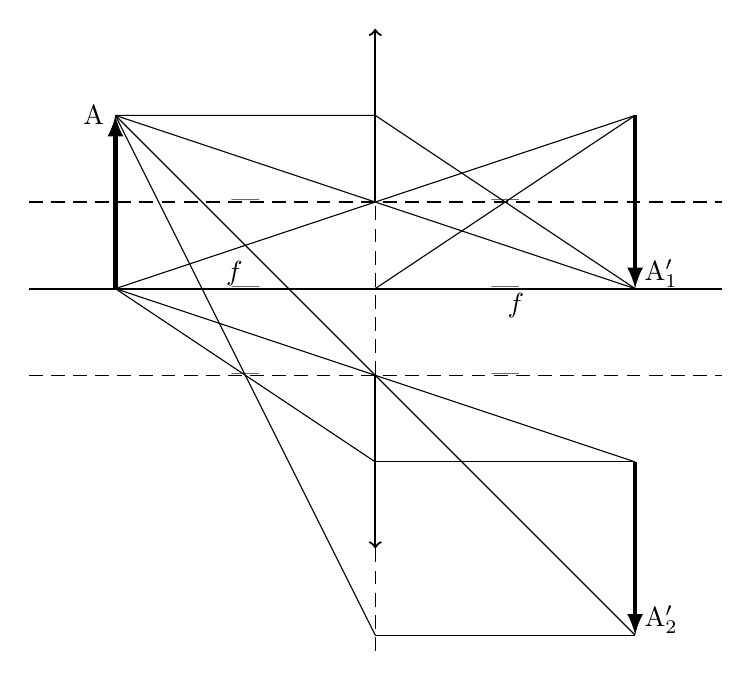
\begin{tikzpicture}[scale=0.55]

    % Def. koordinaadid
    \coordinate (O) at (0,0) ;
    \coordinate (A) at (-8,0) ;
    \coordinate (A') at (8,0) ;
    \coordinate (1) at (0,2);
    \coordinate (2) at (0,6);
    \coordinate (3) at (0,-2);
    \coordinate (4) at (0,-6);
    \coordinate (K) at (-6,4);
    \coordinate (KO) at (-6,0);
    

    % Jooned, t2pid
    \draw[thick] (A) -- (A');
    \draw[thick][->] (1) -- (2);
    \draw[thick][->] (3) -- (4);
    \draw[dash pattern=on5pt off3pt] (-8,2) -- (8,2);
    \draw[dash pattern=on5pt off3pt] (-8,-2) -- (8,-2);
    \draw[dash pattern=on5pt off3pt] (0,-2) -- (0,2);
    \draw[dash pattern=on5pt off3pt] (0, -6) -- (0,-8.5);
    \draw (K) -- (6,0);
    \draw (K) -- (0,4);
    \draw (6,0) -- (0,4);
    
    \draw (KO) -- (6,4);
    \draw (0,0) -- (6,4);
    
    \draw (KO) -- (6,-4);
    \draw (KO) -- (0,-4);
    \draw (6,-4) -- (0,-4);
    
    \draw (K) -- (6,-8);
    \draw (K) -- (0,-8);
    \draw (0,-8) -- (6,-8);
    
    \pgfsetarrowsstart{latex}
    \draw[ultra thick] (K) -- (KO) ;
    \draw[ultra thick] (6,0) -- (6,4) ;
    \draw[ultra thick] (6,-8) -- (6,-4) ;

    % Nurgad ja punktid
    \node[] at (-6.5,4)  {A};
    \node[] at (-3,0)  {|};
    \node[] at (3,0)  {|};
    \node[] at (-3,2)  {|};
    \node[] at (3,2)  {|};
    \node[] at (-3,-2)  {|};
    \node[] at (3,-2)  {|};
    \node[] at (3.25,-0.4)  {$f$};
    \node[] at (-3.25,0.35)  {$f$};
    \node[] at (6.6,0.35)  {$\mathrm{A_1'}$};
    \node[] at (6.6,-7.65)  {$\mathrm{A_2'}$};
    
\end{tikzpicture}
\end{center}
\probend
\bigskip

% S106
\setAuthor{Taavi Pungas}
\setRound{lahtine}
\setYear{2012}
\setNumber{G 4}
\setDifficulty{3}
\setTopic{Geomeetriline optika}

\prob{Fly}
\solueng
The trajectory of the fly during a short time $t$ is a line of length $h=vt$. In the figure we construct the trajectory of the fly’s image. From similar triangles we can find the length of the image’s trajectory $h'$:
$$\frac{h}{a-f}=\frac{h'}{f} \Rightarrow h'=\frac{f}{a-f} h.$$ 
The velocity of the image is therefore
$$v' = \frac{h'}{t} = \frac{f}{a-f} \frac{h}{t} = \frac{f}{a-f} v. $$ 
and it has the opposite direction to the fly’s velocity.
\probend
\bigskip

% S107
\setAuthor{Oleg Košik}
\setRound{piirkonnavoor}
\setYear{2012}
\setNumber{G 1}
\setDifficulty{3}
\setTopic{Geomeetriline optika}

\prob{Mirror}
\solueng
\begin{center}
\includegraphics[width=200pt]{2012-v2g-01-peegel_lah}
\end{center}
A moment $t$ when the acquaintances notice each other is pictured in the figure. By this moment $A$ covered a distance $2-1\cdot t$ and $B$ covered a distance $3,5-1\cdot t$. From similar triangles we get
\[
\frac{1}{3,5-t}=\frac{2-t}{1}.
\] 
We get a quadratic equation that has the solutions $t=\SI{1,5}{s}$ and $t=\SI{4,0}{s}$ where the first of them is the answer.
\probend
\bigskip

% S108
\setAuthor{Tanel Kiis}
\setRound{lõppvoor}
\setYear{2013}
\setNumber{G 1}
\setDifficulty{3}
\setTopic{Geomeetriline optika}

\prob{Lenses}
\solueng
\begin{center}
	\includegraphics[width=0.8\textwidth]{2013-v3g-01-laats_lah2}\\
\end{center}
The whole picture is symmetrical with respect to the optical axis, thanks to this we can only study one side. We construct the path of the rays knowing that the extensions of all the parallel rays going through the concave lens intersect on focal plane.\\
In the figure there are some similar triangles of interest to us:
$$\Delta AF'D \sim \Delta BO'D \sim \Delta CFD$$ 
and 
$$\Delta EOF \sim \Delta AF'O' \sim \Delta BO'F.$$ 
In addition we know the lengths of some of the line segments: $|EO| = R$, $|OF| = f_1$, $|F'O'| = f_2$ and $|CF| = r$. Knowing this we can construct a system of linear equations consisting of four equations.
\[ 
\begin{cases}
\frac{|EO|}{|OF|} = \frac{|AF'|}{F'O}\\
\frac{|EO|}{|OF|} = \frac{|BO'|}{O'F}\\
\frac{|AF'|}{|F'D|} = \frac{|CF|}{|FD|}\\
\frac{|AF'|}{|F'D|} = \frac{|BO'|}{|O'D|},\\
\end{cases}
\] 
\[ 
\begin{cases}
\frac{R}{f_1} = \frac{|AF'|}{f_2}\\
\frac{R}{f_1} = \frac{|BO'|}{\frac{f_1}{2}}\\
\frac{|AF'|}{|O'D| - f_2} = \frac{r}{\frac{f_1}{2} + |O'D|}\\
\frac{|AF'|}{|O'D| - f_2} = \frac{|BO'|}{|O'D|}.\\
\end{cases}
\]
After solving the system we get the result $f_2 = \frac{R}{4r}f_1$.\\

\emph{Alternative solution}
\begin{center}
	\includegraphics[width=0.9\textwidth]{2013-v3g-01-laats_lah3}\\
\end{center}
In this solution we use the thin lens formula $-\frac{1}{f} = \frac{1}{a} - \frac{1}{k}$. There is a minus in front of $f$ because we are dealing with a concave lens and a minus in front of $k$ because it is a virtual image. Using the principle of reversibility of light we instead study the situation where a virtual image $AB$ of object $CF$ appears. In addition we use similar triangles: $\Delta CFO' \sim \Delta ABO'$ and $\Delta DOF \sim \Delta ABF$.
\[ 
\begin{cases}
\frac{|CF|}{|FO'|} = \frac{|AB|}{|BO'|}\\
\frac{|DO|}{|OF|} = \frac{|AB|}{|BF|}\\
-\frac{1}{f_2} = \frac{1}{|FO'|} - \frac{1}{|BO'|},\\
\end{cases}
\]
\[ 
\begin{cases}
\frac{r}{\frac{f_1}{2}} = \frac{|AB|}{|BO'|}\\
\frac{R}{f_1} = \frac{|AB|}{\frac{f_1}{2} - |BO'|}\\
-\frac{1}{f_2} = \frac{1}{\frac{f_1}{2}} - \frac{1}{|BO'|}.\\
\end{cases}
\]
Solving this system of equations we get $f_2 = \frac{R}{4r}f_1$.
\probend
\bigskip

% S109
\setAuthor{Valter Kiisk}
\setRound{lõppvoor}
\setYear{2015}
\setNumber{G 2}
\setDifficulty{3}
\setTopic{Geomeetriline optika}

\prob{Lighting}
\solueng
Let us observe the paths of the outermost rays through the system.
\begin{center}
\includegraphics[scale=1.5]{2015-v3g-02-valgustamine-lah}
\end{center}
After going through the additional lens the rays focus to a point at a distance $f_2$ from the additional lens, meaning at a distance $L-f_2$ from the initial lens. Based on the thin lens formula
\begin{equation}
\frac{1}{a}+\frac{1}{L-f_2}=\frac{1}{f_1}.
\end{equation} 
a point image of this point forms in turn at a distance $a$ from the first lens. From similar triangles we get another two equations:
\begin{equation}
\frac{d_1}{d_0}=\frac{L-f_2}{f_2},
\end{equation} 
\begin{equation}
\frac{d}{a-f_1}=\frac{d_1}{a}.
\end{equation}
Expressing the value $\frac{1}{L-f_2}$ from the first two equations we get
\begin{equation}
\frac{1}{a}+\frac{d_0}{d_1f_2}=\frac{1}{f_1}\implies \frac{d_0}{d_1f_2}=\frac{a-f_1}{af_1}.
\end{equation} 
We can express the value $d_1(a-f_1)/a$ from the last two equations and based on this we get $d=d_0\frac{f_1}{f_2}.$. Therefore the size of the lighted area only depends on the focal length of the additional lens but not on the distance $L$ between the lenses. A lighted area of diameter 2 cm appears if $f_2=f_1d_0/d=\SI{2}{cm}$.
\probend
\bigskip

% S110
\setAuthor{Andreas Valdmann}
\setRound{lahtine}
\setYear{2016}
\setNumber{G 4}
\setDifficulty{4}
\setTopic{Geomeetriline optika}

\prob{Optical fiber}
\solueng
In a long optical fiber only such rays will remain that go through a total internal reflection at the separation surface of the core and the coating. If the light falls on the separation surface with a smaller angle than the critical angle of total internal reflection then both reflection and refraction take place. After several reflections the intensity of such rays will practically decrease to zero because almost all the light has refracted out from the sides of the fiber. The critical angle of total internal reflection $\alpha=\arcsin(n_2/n_1)=\ang{80,5}$. The rays corresponding to the critical angle are travel at an angle $\ang{90}-\alpha$ with respect to the fiber’s axis. After refracting out from the fiber’s end the angle of these rays with respect to the fiber’s axis is $\beta=\arcsin[n_1\sin(\ang{90}-\alpha)]=\arcsin[n_1\cos(\alpha)]$. The light cone’s apex angle $\theta$ is two times bigger than that: $\theta=2\beta=2\arcsin[n_1\cos(\alpha)]=\ang{28}$. Because $\cos(\arcsin(a))=\sqrt{1-a^2}$ then the answer can be presented as $\theta=2\arcsin(\sqrt{n_1^2-n_2^2})$.
\begin{center}
    \includegraphics[width=0.35\textwidth]{2016-lahg-04-kiud}
\end{center}
\probend
\bigskip

% S111
\setAuthor{Andres Põldaru}
\setRound{lahtine}
\setYear{2016}
\setNumber{G 5}
\setDifficulty{4}
\setTopic{Geomeetriline optika}

\prob{Three lenses}
\solueng
All of the three lenses have the same focal length because they have one common focal point which is the center of the triangle. The triangles $\triangle ACD$ and $\triangle CEF$ are similar because they are right triangles that have the same angle at the common tip $C$. Therefore $\frac{|AD|}{|AC|}=\frac{|EF|}{|EC|}$ where $|AD| = \frac{|AC|}{2} = f$. 
\begin{center}
	{\def\l{5}
	\pgfmathsetmacro\cos{cos(30)}
	\pgfmathsetmacro\tan{tan(30)}
	\begin{tikzpicture}[scale=0.7]
	\coordinate (A) at (-\l*\tan,0);
	\coordinate (B) at (\l*\cos+\l/2*\tan,0);
	\draw[Stealth-Stealth] (0,0) node[below]{C} -- ++(30:5) node[above]{E};
	\draw[Stealth-Stealth] (30:\l) -- ++(-90:5) node[below]{G};
	\draw[Stealth-Stealth] (0,0) -- ++(-30:\l);
	\draw (0,0) -- ++(210:2.5) node[below]{D} -- ++(30:0.3) arc (30:120:0.3) -- ++(-60:0.3)-- (A) -- (0,0) -- (\l*\cos,0) node[below left]{F};
	\node at (B) {\textbullet} (B) node[anchor=west] {B};
	\node at (A) {\textbullet} (A) node[anchor=east] {A};
	\draw[decorate,decoration={brace,raise=2pt,amplitude=6pt}] (A)  -- node[above right = 7pt and -10pt]{$2f$} (0,0) ;
	\draw[decorate,decoration={brace,raise=2pt,amplitude=6pt}] (210:2.5)  -- node[below left = 2pt and 6pt]{$f$} (A);
	\draw[decorate,decoration={brace,raise=2pt,amplitude=6pt}] (B)  -- node[below right = 7pt and -8pt]{$f$} (\l*\cos,0) ;
	\end{tikzpicture}}
\end{center}
We can conclude that the point $A$ is located on the focal planes of both of the lenses $CE$ and $CG$. If parallel rays fall on a lens then they focus to one point on its focal plane, so when thinking the other way around, the rays originating from one point of the focal plane have to be parallel after going through the lens. The angle of these parallel rays can be determined if we draw one line from the point $A$ through the center of lens $CE$ or $CG$. A ray going through the center of a lens does not refract and moves forward along the same direction. In the bottom figure the ray $AH$ goes through the center of a lens and the other rays are constructed so that after going through a lens they are parallel to it.\\
After going through the first lens the parallel rays falling on the lens $EG$ focus on one point $J$ on the focal plane. To find this point we draw a ray going through the center $F$ of the lens $EG$ that is parallel to the ray $AH$ and we find the ray’s intersection point $J$ with the focal plane. From the figure it can be seen that not a single ray reaches the point $B$ because they focus to the point $J$ and there are no vertical rays. For the lens $CG$ the construction is the same only that it is reflected with respect to $AB$ and therefore no light reaches the point $B$ from there either.
\begin{center}
	{\def\l{5}
	\pgfmathsetmacro\cos{cos(30)}
	\pgfmathsetmacro\tan{tan(30)}
	\begin{tikzpicture}[scale=0.9]
	\usetikzlibrary{calc};
	\pgfmathsetmacro\tanb{sqrt(3)/7}
	\pgfmathsetmacro\k{\l*\cos+\l*\tan}
	\coordinate (A) at (-\l*\tan,0);
	\coordinate (B) at (\l*\cos+\l/2*\tan,0);
	\coordinate (H) at ($\k*(1,\tanb)+(A)$);
	\coordinate (J) at ($(\l*\cos,0)+\l*\tan/2*(1,\tanb)$);
	\draw[Stealth-Stealth] (0,0) node[below left]{C} -- ++(30:5) node[above]{E};
	\draw[Stealth-Stealth] (30:\l) -- ++(-90:5) node[below]{G};
	\draw[Stealth-Stealth] (0,0) -- ++(-30:5);
	\node at (B) {\textbullet} (B) node[anchor=west] {B};
	\node at (A) {\textbullet} (A) node[anchor=east] {A};
	\draw (A) -- (H) node{\textbullet} node[above left = -3pt and 0pt]{H};
	\draw (\l*\cos,0) node[left]{F} -- (J) node {\textbullet} node[above right = -5pt and 0pt]{J};
	\draw (H) -- (J);
	\draw (A) -- (30:0.5) -- ++({(\l-0.5)*\cos},{(\l-0.5)*\cos*\tanb}) -- (J);
	\draw (A) -- (30:4.5) -- ++({(\l-4.5)*\cos},{(\l-4.5)*\cos*\tanb}) -- (J);
	\end{tikzpicture}}
\end{center}
\emph{Alternative solution}\\
Analogically we can also observe the situation where there is a light source in the point $B$. If the rays originating from the point $A$ reach the point $B$ then the rays originating from the point $B$ also have to reach the point $A$. The point $B$ is on the focal plane of the lens $EG$ and creates a parallel beam. Similarly to the previous solution after going through the second lens this beam focuses on one point of the focal plane of this lens that is not $A$. The focal plane is parallel to the lens and if the rays focus to a point different from $A$ on this plane then therefore no light reaches the point $A$.
\probend
\bigskip

% S112
\setAuthor{Eero Vaher}
\setRound{piirkonnavoor}
\setYear{2017}
\setNumber{G 5}
\setDifficulty{4}
\setTopic{Geomeetriline optika}

\prob{Missing lens}
\solueng
The concave lens creates a virtual image of the object and the convex lens creates a real image of the virtual image. Knowing the location and focal points of the convex lens and the location of the real image it is possible to find the location of the virtual image (in the image it is depicted with blue; three rays are pictured but for constructing two will suffice). Knowing the locations of the object and the virtual image created by the concave lens it is easy to find the location of the lens and its focal point that is on the same side as the object.\\
\begin{resizebox}{\linewidth}{!}{
		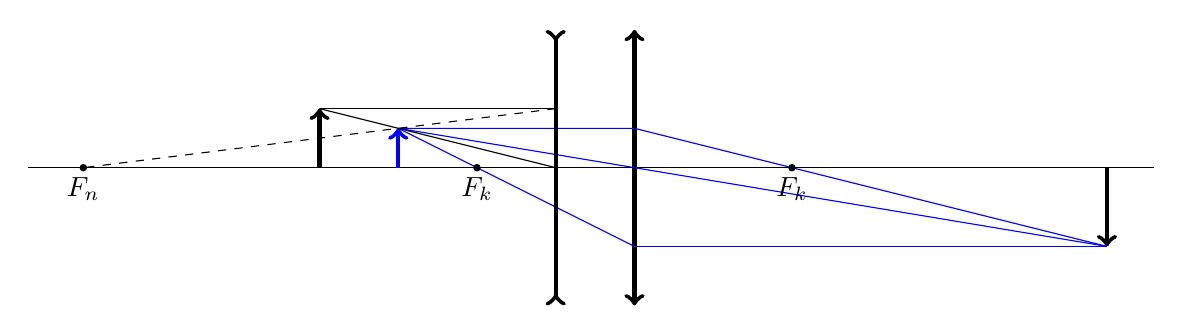
\begin{tikzpicture}
		\pgfmathsetmacro{\fk}{2}
		\pgfmathsetmacro{\tk}{3*\fk}
		\pgfmathsetmacro{\nk}{1/(1/\fk-1/\tk)}
		\pgfmathsetmacro{\a}{2*\fk}
		\pgfmathsetmacro{\h}{0.5}
		\pgfmathsetmacro{\htk}{\tk/\nk*\h}
		\pgfmathsetmacro{\ha}{1.5*\h}
		\pgfmathsetmacro{\nl}{\nk-\h/(\h-\ha)*(\nk-\a)}
		\pgfmathsetmacro{\fn}{\nk-\h/(\h-\ha)*(\nk-\nl)}
		\coordinate (TK) at (\tk, -\htk);
		\coordinate (NK) at (-\nk, \h);
		\coordinate (A) at (-\a, \ha);
		\draw (-1.1*\fn, 0) -- (1.1*\tk, 0);
		\draw[<->, ultra thick] (0,3.5*\h) -- (0,-3.5*\h);
		\draw[->, ultra thick] (\tk, 0) -- (TK);
		\draw[->, ultra thick, blue] (-\nk, 0) -- (NK);
		\draw[blue] (TK) -- (NK);
		\draw[blue] (TK) -- (0,-\htk);
		\draw[blue] (0,-\htk) -- (NK);
		\draw[blue] (TK) -- (0,\h) -- (NK);
		\draw[fill] (-\fk, 0) circle (0.02*\fk) node[below] {$F_k$};
		\draw[fill] (\fk, 0) circle (0.02*\fk) node[below] {$F_k$};
		\draw[->, ultra thick] (-\a, 0) -- (A);
		\draw[>-<, ultra thick] (-\nl, 3.5*\h) -- (-\nl, -3.5*\h);
		\draw (-\nl, 0) -- (A) -- (NK);
		\draw (A) -- (-\nl, \ha);
		\draw[dashed] (-\nl, \ha) -- (-\fn,0);
		\draw[fill] (-\fn, 0) circle (0.02*\fk) node[below] {$F_n$};
		\end{tikzpicture}}
\end{resizebox}
\probend
\bigskip

% S113
\setAuthor{Andreas Valdmann}
\setRound{lõppvoor}
\setYear{2014}
\setNumber{G 4}
\setDifficulty{5}
\setTopic{Geomeetriline optika}

\prob{Periscope glasses}
\solueng
\osa Because the entering and exiting rays are perpendicular to the surface of the prism then their direction does not change on the separation surface of environments. If a ray falls on the prism on the section $AB$ then it first reflects on the upper face of the prism, next on the bottom face and exits from the prism through the right face (see figure). If a ray falls on the prism on the section $BC$ then it reflects on the upper face, then on the right face, after that exits through the bottom face and does not reach the eye. If a ray falls on the prism on the section $CD$ then it first reflects on the right face, then on the upper face and exits again through the bottom face. 
\begin{center}
  \includegraphics[width=0.8\textwidth]{2014-v3g-04-periskoopprillid_lahendus_joonis1}
\end{center}
\osa Let us observe a ray that enters the prism on the section $AB$. Because the entering ray is perpendicular to the surface a right triangle $AKL$ is formed (see figure). One of the acute angles of the triangle is $\varphi$ and therefore the value of the other acute angle is $\ang{90}-\varphi$. Because the latter angle is the supplementary angle for the angle of incidence of the first reflection then the angle of incidence is also $\varphi$. From the law of reflection it is concluded that the first angle of reflection is also $\varphi$. Because the ray exiting the prism is parallel to the upper face of the prism then for the second reflection $\varphi$ is the supplementary angle of the angle of reflection and therefore the supplementary angle of the angle of incidence as well. We see that the acute angles of the right triangle $KLM$ are $\varphi$ and $2\varphi$. Because the sum of a triangle’s interior angles is $\ang{180}$ then $\varphi=(\ang{180}-\ang{90})/3=\ang{30}$.
\begin{center}
  \includegraphics[width=0.65\textwidth]{2014-v3g-04-periskoopprillid_lahendus_joonis2}
\end{center}
\emph{Note}. Now that the acute angle of the prism has been found we can make certain that if a ray entering the surface perpendicularly reflects from the bottom or right face of the prism then these reflections are total. From the previous subtask it can be seen that in these cases the angle incidence is $\ang{90}-\varphi=\ang{60}$. The critical angle of a total internal reflection is $\alpha=\arcsin(1/n)=\ang{42}$. The angle of incidence $\ang{60}$ is bigger than this which means that a total internal reflection takes place.\\
\osa If a ray enters the prism from the point $B$ then the exiting ray goes through the point $D$ (see figure). \\
\emph{Note}. The direction of the exiting ray is not unequivocally determined in this case but in this solution it does not matter.\\
Using the value of $\varphi$ from the previous subtask it can be seen that the triangles $ABL$ and $BDL$ are each other’s reflections with respect to the section $BL$ (meaning that these triangles are congruent). Therefore the lengths of the sections $AB$ and $BD$ are equal from which we can conclude that $|AB|=l/2$. If a ray enters the prism from the point $C$ then it reflects straight back from the point $O$ and exits the prism from the point $C$. From right triangles we get that $|AO|=\cos(\ang{30})|AD|$ and $|AC|=\cos(\ang{30})|AO|$ meaning that the distance of the point $C$ from the point $A$ is $|AC|=\cos^2(\ang{30})|AD|=\frac{3}{4}l$. 
\begin{center}
  \includegraphics[width=0.65\textwidth]{2014-v3g-04-periskoopprillid_lahendus_joonis3}
\end{center}
\osa A text would be seen as a reflection if we use one plane mirror. To see the text in the right way a system has to be used where an even number of reflections take place.
\probend
\bigskip

% S114
\setAuthor{Mihkel Kree}
\setRound{lahtine}
\setYear{2015}
\setNumber{G 5}
\setDifficulty{5}
\setTopic{Geomeetriline optika}

\prob{Lens}
\solueng
Let us first notice that the rays AA’ and BB’ going through the center of the lens do not refract. Therefore the center of the lens O is located in the intersection of the sections AA’ and BB’. Let us also notice that the ray AB is refracted into the ray A’B’. So, extending the sections AB and A’B’ we find their intersection X. With this we have constructed the plane of the lens OX. We find the optical axis of the lens if we draw a line s perpendicular to the plane of the lens through the center of the lens O. To find the focal point F we can construct a ray AC parallel to the main axis that refracts through the focal point. 
\begin{center}
\includegraphics[width=\textwidth]{2015-lahg-05-laatsLahendus}
\end{center}
\probend
\bigskip

% S115
\setAuthor{Sandra Schumann}
\setRound{lõppvoor}
\setYear{2018}
\setNumber{G 3}
\setDifficulty{5}
\setTopic{Geomeetriline optika}

\prob{Mirror base}
\solueng
Let us notice that if the refractive index of the environment increases but the refractive index of the lens stays the same then based on the formula the focal length of the lens increases. Therefore the only way for the light rays to converge on the same point after filling the vessel is for the rays in the water to reflect from the mirror on the base and then converge on the same point as before.\\
The distance of the lens from the base of the vessel is $l = \SI{10}{cm}$. Let the focal length of the lens in the air be $f$. Its focal length in the water is therefore $2l-f$. Based on the formula we get that
\[ \frac{f}{2l-f} = \frac{n_g n_0 - n_0 n_w}{n_g n_w - n_0 n_w}\Rightarrow \] 
\[ f(n_g n_w - n_0 n_w) = (2l-f)(n_g n_0 - n_0 n_w)\Rightarrow \]
\[ n_g n_w f - n_0 n_w f = 2l n_g n_0 - 2l n_0 n_w - n_g n_0 f + n_0 n_w f\Rightarrow \]
\[ f (n_g n_w + n_g n_0 - 2 n_0 n_w) = 2l n_0 (n_g - n_w)\Rightarrow \]
\[ f = \frac{2l n_0 (n_g - n_w)}{n_g n_w + n_g n_0 - 2 n_0 n_w}. \]
Therefore the focal length of the lens
\[ f = \frac{\num{2} \cdot \SI{10}{cm} \cdot \num{1,0} \cdot (\num{1,49} - \num{1,33})}{\num{1,49}
\cdot \num{1,33} + \num{1,49} \cdot \num{1,0} - \num{2} \cdot \num{1,0} \cdot \num{1,33}} = \SI{3,94}{cm}
\approx \SI{4}{cm}. \]
\probend
\bigskip

% S116
\setAuthor{Eero Vaher}
\setRound{piirkonnavoor}
\setYear{2015}
\setNumber{G 8}
\setDifficulty{6}
\setTopic{Geomeetriline optika}

\prob{Focal length}
\solueng
Let us propose a light ray that is coming from the left falls on the lens, it has the direction parallel to the optical axis and is at a distance $d$ from it. Entering the lens the light does not change its travel direction because it falls on the lens perpendicularly to its surface. The silvered surface acts as a convex mirror that has a focal length $\frac{R}{2}$. If the reflected ray is at an angle $\alpha$ with respect to the optical axis then the angle between the ray exiting the lens and the optical axis according to the law of refraction is $\sin\gamma=n\sin\alpha$. Because the lens is thin then the points where the light ray reflected and where it refracted are positioned very close to each other. Therefore we can write
\[ d=\frac{R}{2}\tan\alpha=f\tan\gamma. \] 
In the case of a thin lens the radius of its concave part is significantly bigger from the focal length, this allows us to use the paraxial approximation $\alpha\approx\sin\alpha\approx\tan\alpha$ and $\gamma\approx\sin\gamma\approx\tan\gamma$. In result we get
\[ f=\frac{R}{2n}. \] 
It should be known that the expression for the focal length of a spherical mirror only applies for small angles of reflection. In the case of big angles of reflection a spherical aberration occurs and it is not possible to talk about one focal point. 
\begin{center}
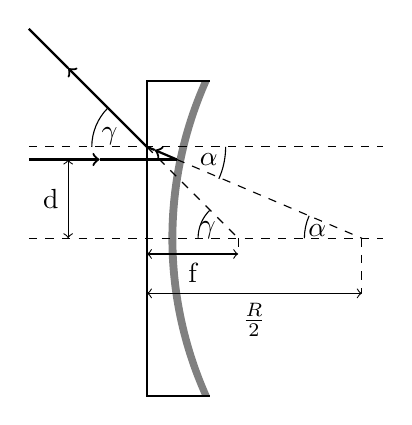
\begin{tikzpicture}[scale=1]
\def\tmp{65.92}
\fill [gray] (0.7,2) arc (90+\tmp:270-\tmp:4.9) -- (0.8,-2) -- (0.8,-2) arc (270-\tmp:90+\tmp:4.9) -- (0.7,2);
\draw[thick] (0.8,-2) -- (0,-2) -- (0,2) -- (0.8,2);
\draw[dashed] (-1.5,0) -- (3,0);
\draw[->,thick] (-1.5,1) -- (-0.6,1);
\draw[thick] (-0.6,1) -- (0.38,1);
\draw[dashed] (0.38,1) -- (2.73,0);
\draw[->,thick] (0.38,1) -- (0.1,1.12);
\draw[thick] (0.1,1.12) -- (0,1.16);
\draw[->,thick] (0,1.16) -- (-1,2.16);
\draw[thick] (-1,2.16) -- (-1.5,2.66);
\draw[dashed] (0,1.16) -- (1.16,0);
\draw[<->] (-1,0) -- (-1,1);
\node [left] at (-1,0.5) {d};
\draw[dashed] (-1.5,1.16) -- (3,1.16);
\node [left] at (-0.25,1.3) {$\gamma$};
\draw (-0.7,1.16) arc (180:135:0.7);
\node [right] at (0.55,1) {$\alpha$};
\draw (1,1.16) arc (0:-24:1);
\draw[dashed] (1.16,0) -- (1.16,-0.2);
\draw[<->] (0,-0.2) -- (1.16,-0.2);
\node [below] at (0.58,-0.2) {f}; 
\draw[dashed]  (2.73,0) -- (2.73,-0.7);
\draw[<->] (0,-0.7) -- (2.73,-0.7);
\node[below] at (1.36,-0.7) {$\frac{\text{R}}{2}$};
\node[left] at (2.4,0.1) {$\alpha$};
\draw (2,0) arc (180:156:0.7);
\node[left] at (1,0.1) {$\gamma$};
\draw (0.65,0) arc (180:135:0.5);
\end{tikzpicture}
\end{center}
\probend
\bigskip

% S117
\setAuthor{Jaan Kalda}
\setRound{lõppvoor}
\setYear{2012}
\setNumber{G 6}
\setDifficulty{7}
\setTopic{Geomeetriline optika}

\prob{Tube}
\solueng
Let us first notice that the image of the point light source appears at the following distance from the lens:
$$l=\left(\frac 1{36}-\frac 1{60}\right)^{-1}\SI{}{mm}=\SI{90}{mm},$$ 
meaning on the screen. If there were two plane mirrors in place of the reflecting cylindrical walls then an infinite sequence of the light source’s images would appear (reflection, reflection’s reflection and so on), where the distance between two neighboring images is equal to the distance between the mirrors, 12 mm. Let us now observe the cylindrical case. A ray lying on the plane of the figure has the same path as it would have in the case of a flat mirror, meaning that on the plane of the figure the images also occur in a periodical sequence where the distance between the images is 12 mm. The plane of the figure can be randomly turned around the symmetry axis of the system; this means that the images are actually “smudged” along a concentric circle of radius $n\times\SI{12}{mm}$ where $n$ is an integer. The lens creates a $\frac{90}{60}$ times magnified image of these circles on the screen where the radius of the concentric circles is $R=n\times \SI{18}{mm}$.
\probend
\bigskip

% S118
\setAuthor{Valter Kiisk}
\setRound{lõppvoor}
\setYear{2013}
\setNumber{G 7}
\setDifficulty{7}
\setTopic{Geomeetriline optika}

\prob{Microscope}
\solueng
In the first sharp position where the lens is closer to the object than the sensor (meaning the magnification is $>1$) let the distance of the lens from the object be $a$ and from the sensor $b$. The linear magnification of the image is therefore $k=b/a$. In the second position the named distances are simply the other way around and the magnification is respectively $l=a/b$. Thus, $25=k/l=b^2/a^2$.\\
Let us now analyze the question of illumination based on the distances of the first position. Since the linear magnification is $k$ then the factor describing the area change is $k^2$. Besides the size of the image its brightness is also affected by the amount of light that goes through the lens. From each point of the observable object a light originates that is more or less evenly dispersed over all the directions, thus, the radiative flux going through the lens is proportional to the area of the imaginary sphere’s surface that is cut out by the aperture of the lens: $\Omega=d^2/a^2$, where $d$ is the diameter of the lens. In conclusion we get that the brightness of the image is proportional to the value $\Omega/k^2=d^2/b^2\propto b^{-2}$. In the second position where the lens is closer to the lens the same factor is respectively $a^{-2}$, therefore in this case the brightness of the image is $a^{-2}/b^{-2}=b^2/a^2=25$ times bigger.
\probend
\bigskip

% S119
\setAuthor{Erkki Tempel}
\setRound{lahtine}
\setYear{2014}
\setNumber{G 7}
\setDifficulty{7}
\setTopic{Geomeetriline optika}

\prob{Optical diagram}
\solueng
\begin{center}
\includegraphics[width=0.7\textwidth]{2014-lahg-07-optilineskeemlahendus_ing}
\end{center}
Initially parallel rays converge on the focal plane (point A) after going through the lens. Because the bottom ray does not refract it has to go through the center of the lens. Therefore the lens 1 is parallel to the drawn focal plane (the ray goes through the points A and F) and goes through the point $\text{O}_1$. Because we are dealing with two identical lens and their focal points are at the point F then a circle of radius $\text{FO}_1$ intersects with the bottom ray at the point $\text{O}_2$ which is the center of the second lens. Now we can easily draw the second lens because we know the location of the bottom ray’s refraction point and the lens’ center.
\probend
\bigskip

% S120
\setAuthor{Valter Kiisk}
\setRound{lõppvoor}
\setYear{2016}
\setNumber{G 6}
\setDifficulty{7}
\setTopic{Geomeetriline optika}

\prob{Magnifier}
\solueng
The central region of the hemisphere’s convex surface can be looked at as a separate thin lens. Its focal length $f$ and distance from the paper’s surface (equal to the radius $R$ of the convex surface) determine the magnification of the image. To determine the focal length of the lens equivalent to the hemisphere we observe a light ray that moves parallel to the optical axis and after refraction converges to the focal point (see figure). If the light ray travels close to the optical axis then all the angles occurring during refraction are small, meaning we get the condition
\[
\alpha R\approx f\varphi.
\]
Probably
\[
\varphi = \alpha - \beta=\alpha-\alpha/n=\alpha(1-1/n).
\]
Combining these relations the angles cancel out and we get $f=nR/(n-1)$. The distance of the object (paper’s surface) is probably $R$, moreover $f > R$, therefore a virtual image appears somewhere behind the paper. All the distances nevertheless have the same order of magnitude as $R$, thus, a magnification looked at at a great distance (meaning angular magnification) is practically the same as a linear magnification $y/y_0$. From the similar triangles that form during the construction of the image we get
\[
\frac{y}{y_0}=\frac{f}{f-R}=n=\num{1.5}.
\]  
\begin{center}
	\includegraphics[scale=1.2]{2016-v3g-06-luup-lah}
\end{center}
\probend
\bigskip

% S121
\setAuthor{Andreas Valdmann}
\setRound{lõppvoor}
\setYear{2016}
\setNumber{G 8}
\setDifficulty{8}
\setTopic{Geomeetriline optika}

\prob{Corner mirror}
\solueng
Let us first study the formation of an image in a flat mirror. The situation is pictured in the figure 1 from top view. A is Juku’s open eye and A$'$ its image. A closed eye and its image are respectively B and B$'$. We see that if one closes the right eye then with respect to the observer the right eye in the mirror seems to be closed as well. 
\begin{figure*}[h]
	\centerline{\includegraphics[scale=1.2]{2016-v3g-08-nurgapeegel_j1}}
	\caption{Image in a plane mirror}
\end{figure*}
Let one of the mirror from the three be horizontal and the two rest vertical, moreover Juku looks directly to the line between the vertical mirrors. In the figure 2 this situation is pictured from top view. Let us observe the effect of the vertical mirrors. First, we construct the image A$'$ of the eye A in the left mirror. Next we construct the image A$''$ of the image A$'$ in the right mirror. We do the same when constructing the image B$''$ and notice that this time the right and left side of the reflection are switched and the eye that seems to be closed is the left one.\\
Let us now take into consideration the impact of the horizontal mirror. In the figure 3 the second order image A$''$ and its image A$'''$ are in front view. We see that the horizontal mirror reverses the picture. Therefore Juku sees himself from the corner mirror as the image A$'''$ from the figure 3. 
\begin{figure*}[h]
	\centerline{\includegraphics[scale=1.2]{2016-v3g-08-nurgapeegel_j2}}
	\caption{Image in two mirrors}
\end{figure*}
\begin{figure*}[h]
	\centerline{\includegraphics[scale=1.1]{2016-v3g-08-nurgapeegel_j3}}
	\caption{Reflection from horizontal mirror}
\end{figure*}
\probend
\bigskip

% S122
\setAuthor{Jaan Kalda}
\setRound{lõppvoor}
\setYear{2015}
\setNumber{G 7}
\setDifficulty{9}
\setTopic{Geomeetriline optika}

\prob{Circle and eclipse}
\solueng
The center $O$ of the lens is the intersection point of the tangents drawn from the ring and the eclipse because intersection points have to be in pairs with original images and the lines connecting them have to go through the center. To find the plane of the lens we choose two points on the ring, $A$ and $B$, and we find their images $A'$ and $B'$ on the eclipse to be the intersection points of lines $AO$ and $BO$ and the eclipse. If the original from the two intersection points of the ring is the one that is further from the lens then its image is the one that is closer to the lens (and the other way around), because a real image is turned upside down. The ray $AB$ has to refract in the mirror into the ray $A'B'$, the refraction point gives us a point $L$ on the lens and the line $OL$ is the plane of the lens. We find the optical axis $o$ to be the perpendicular drawn on the line $OL$ from the point $O$. To find the focal point we draw a line from the point $A$ that is parallel to $o$ and refracts into a ray going through the point $A'$. The intersection point of this ray with $o$ gives us the focal point $F$.
\begin{center}
\includegraphics[width=\textwidth]{2015-v3g-07-ellips_lah}
\end{center}
\probend
\bigskip

% S123
\setAuthor{Ardi Loot}
\setRound{lõppvoor}
\setYear{2017}
\setNumber{G 8}
\setDifficulty{9}
\setTopic{Geomeetriline optika}

\prob{Camera}
\solueng
It is clear that since the northern lights are far away then the photosensitive element has to be in the focal point of the initial lens to create a sharp image, meaning at the distance $f=\SI{14}{cm}.$. Because the ray going through the center of the lens does not change direction we get the initial view angle to be $2\alpha=2\arctan\left(h/f\right)$.
\begin{center}
	\includegraphics[width=10cm]{2017-v3g-08-skeem__telephoto}
\end{center}
A diagram of a compact camera is pictured in the figure. For simplification let us observe the situation the other way around, the observable object is in place of the photosensitive element and the image is constructed in infinity (principle of reversibility of light). The concave lens that is at the distance $d$ from the convex lens creates a virtual image $A'$ of the object $A$. This virtual image is observed with the convex lens that constructs an image of it in infinity. We can write down the following equations:
\begin{eqnarray}
\frac{1}{k_{1}}-\frac{1}{a_{1}} = \frac{1}{f_{1}}, \label{2017-v3g-08-eq:telelens-eq1}\\
k_{1}+d = f_{2},\\
a_{1}+d = L_{m}.
\end{eqnarray}
With the first of these we find the location of the virtual image created by the concave lens. The second equation guarantees that the convex lens constructs an image of it in infinity. The third equation ensures that the whole system is compact. In addition to the aforementioned equations the initial view angle of the camera also needs to be preserved. For this we notice that the angle given in the figure $\measuredangle A'O_{2}F_{2}=\alpha$. Because of this we can write down:
\begin{equation}
\frac{h'}{f_{2}}=\frac{h}{f},
\end{equation}
where $h'$ is the height of the image $A'$ that we can find from the similarity of triangles $OAO_{1}$ and $F_{2}A'O_{1}$
\begin{equation}
h'=h\frac{k_{1}}{a_{1}.}\label{2017-v3g-08-eq:telelens-eq2}
\end{equation}
Solving the system of equations made from the equations (1) – (5) we get
\begin{eqnarray*}
f_{1} & = & \frac{f_{2}f(L_{m}-f_{2})}{\left(f-f_{2}\right)^{2}}\approx\SI{1.39}{cm},\\
d & = & \frac{f_{2}(f-L_{m})}{f-f_{2}}\approx\SI{1.91}{cm}.
\end{eqnarray*}
\probend
\bigskip

% S124
\setAuthor{Jaan Kalda}
\setRound{lõppvoor}
\setYear{2014}
\setNumber{G 10}
\setDifficulty{10}
\setTopic{Geomeetriline optika}

\prob{Glass cylinder}
\solueng
\begin{wrapfigure}{r}{0.35\textwidth}%
\includegraphics[trim = 0mm 0mm 12mm 0mm, clip, width=1\linewidth]{2014-v3g-10-silinder}
\end{wrapfigure}
Let the marked point be $A$ and let us assume that the ray going through it refracts in a point $B$ so that it is directed away through a point $C$ (see figure). Observing from far away from the direction of $BC$ we see the location of the dark point to be the point $B$. Let us see how the travel direction of the ray $BC$, that is described with the angle between $AO$ and $BC$, $2\alpha-\beta$, depends on the initial travel direction $\alpha$ of the ray:
$$2\alpha-\beta= 2\alpha-\arcsin (n\sin\alpha).$$
For the initial position of the cylinder $2\alpha-\arcsin (n\sin\alpha) =0$. One of its solution $\alpha=0$ gives us the middle virtual point and the two outer dark points meet the solutions of the equation $\sin(2\alpha)=n\sin\alpha$ in the interval $-45^\circ <\alpha<45^\circ$. If the cylinder were now turned by an angle $\delta$ then the virtual points meet the solutions of the equation
$$2\alpha-\arcsin (n\sin\alpha) =\delta$$
On the left side of the equation there is a function that in the case of small angles acts as $(2-n)\alpha$; in the case of bigger angles the relative effect of the second addend increases. Therefore if $2>n$ we are dealing with an increasing function in the case of small angles, this function starts to decrease in the case of bigger angles; if $2<n$ it is, however, a monotonically decreasing function. Since in the case of $\delta=0$ there are three solutions then we have to be dealing with the first case, $2>n$. In the case of such rotation angles $\delta$ that are bigger from the relative maximum of this function the equation only has one solution. The function reaches the absolute maximum in the limit case of a total internal reflection
$$n\sin\alpha=-1,$$
that gives us the rotation angle 
$$90^\circ-2\arcsin \frac 1n=\SI{15}{}^\circ\Rightarrow n=1/\sin \ang{37,5} = \SI{1,64}{}.$$
\probend
\bigskip

% S125
\setAuthor{Koit Timpmann}
\setRound{piirkonnavoor}
\setYear{2013}
\setNumber{G 1}
\setDifficulty{1}
\setTopic{Kinemaatika}

\prob{Train}
\solueng
Let the maximal velocity of the train be $v$ and the total driving time $t$. During acceleration the average velocity is $v/2$ and the time of the acceleration is $\frac{2t}{5}$. The braking takes the time $\frac{t}{5}$ and during this the average velocity is also $v/2$. The average velocity of the whole drive is therefore
$$v_k = \frac{\frac{2t}{5} \frac{v}{2}+\frac{2t}{5} v + \frac{t}{5} \frac{v}{2}}{t} = \frac{7}{10} v.$$
From here $v=\frac{10}{7}v_k \approx \SI{51}{km/h}$.
\probend
\bigskip

% S126
\setAuthor{Mihkel Kree}
\setRound{lahtine}
\setYear{2015}
\setNumber{G 1}
\setDifficulty{2}
\setTopic{Kinemaatika}

\prob{Train whistle}
\solueng
Let $L$ be the distance of the locomotive from the station manager at the moment when the engine driver starts to blow the whistle. The time it takes the sound to travel to the station manager is in this case $\tau_\text{A}=L/c$. When the whistling stops the distance of the locomotive from the station manager is $L-vt_0$ where $v$ is the velocity of the train. The time it takes for the sound to travel from that distance is $\tau_\text{B}=(L-vt_0)/c$. Let us say that the engine driver starts blowing the whistle at the moment $\tau_0$ and finishes at the moment $\tau_0+t_0$. The station manager hears the beginning of the whistle at the moment $\tau_0+\tau_\text{A}$ and the finish of the whistle at the moment $\tau_0+t_0+\tau_\text{B}$. The difference of these moments of time $t_1$ is of course the whistle time measured by the manager. Therefore we get the equation $t_1 = t_0+\tau_\text{B}-\tau_\text{A} = t_0 - \frac{v}{c}t_0$ where $v = \frac{t_0-t_1}{t_0}c = \SI{34}{m/s}$.
\probend
\bigskip

% S127
\setAuthor{Erkki Tempel}
\setRound{piirkonnavoor}
\setYear{2015}
\setNumber{G 1}
\setDifficulty{2}
\setTopic{Kinemaatika}

\prob{Freight train}
\solueng
Let us find the times during which the train slowed down and accelerated:
\[ t_p = \frac{v - v_h}{a_p},\quad t_k = \frac{v-v_h}{a_k}. \]
During this time the train covered the distance
\[ s_p = \frac{v^2-v_h^2}{2a_p}, \quad s_k = \frac{v^2-v_h^2}{2a_k}. \]
Driving evenly with 72 km/h the train would have covered this distance with the time
\[ t_{py} = \frac{s_p}{v},\quad t_{ky} =\frac{s_k}{v}. \]
Therefore the loss of time during slowing down and acceleration is
\[ \Delta t_p =  t_{p} - t_{py}, \quad\Rightarrow\quad \Delta t_p = \frac{(v-v_h)^2}{2va_p}=\SI{28,125}{s},\]
\[ \Delta t_k =  t_{k} - t_{ky}, \quad\Rightarrow\quad \Delta t_k = \frac{(v-v_h)^2}{2va_k}=\SI{56,25}{s}.\]
Because the train was late by $\Delta t$ we can find the time $\Delta t_h$ that the train lost when driving evenly:
\[ \Delta t_h = \Delta t - \Delta t_p - \Delta t_k = \SI{215,625}{s}. \]
If the train drove slowly (18 km/h) and covered the distance $s_h$ then the time it took to cover it was
\[ t_h = \frac{s_h}{v_h}. \] 
Driving with a speed 72 km/h the train would have covered that distance with a time
\[ t_{hy} = \frac{s_h}{v}. \]
Knowing that $\Delta t_h = t_{hy} - t_h$ we can express the distance $s_h$:
\[ s_h = \frac{vv_h\Delta t_h}{v-v_h} = \SI{1437,5}{m} \approx \SI{1,4}{km}.\]
\probend
\bigskip

% S128
\setAuthor{Sandra Schumann}
\setRound{lahtine}
\setYear{2017}
\setNumber{G 1}
\setDifficulty{2}
\setTopic{Kinemaatika}

\prob{Ambulance}
\solueng
Let the velocity of the ambulance be $v$ and the frequency of the sound made by the car $f_0$. Let us apply the formula for two cases: when the car approaches and when it retreats. 
When the car approaches:
\[f_1 = \left(\frac{v_s}{v_s - v}\right)f_0.\]
When it retreats:
\[f_2 = \left(\frac{v_s}{v_s + v}\right)f_0.\]
Because the difference of sound frequencies by six tones meets a two time difference in the frequencies then one tone difference meets a $2^{\frac 1 6}$ time difference and one and a half tone difference meets a $\left(2^{\frac 1 6}\right)^{\frac 3 2} = 2^{\frac 1 4}$ time difference. Therefore we get:
\[2^{\frac 1 4} = \frac{f_1}{f_2} = \frac{(\frac{v_s}{v_s - v})f_0}{(\frac{v_s}{v_s + v})f_0} = \frac{v_s + v}{v_s - v},\]
\[v_s + v = 2^{\frac 1 4}v_s - 2^{\frac 1 4}v,\]
\[(2^{\frac 1 4} + 1)v = (2^{\frac 1 4} - 1)v_s,\]
\[v = \frac{2^{\frac 1 4} - 1}{2^{\frac 1 4} + 1}v_s = \frac{2^{\frac 1 4} - 1}{2^{\frac 1 4} + 1} \cdot \SI{343}{\meter\per\second} = \SI{29.64}{\meter\per\second} = \SI{107}{\kilo\meter\per\hour}. \]
We get the answer $\SI{107}{\kilo\meter\per\hour}$.
\probend
\bigskip

% S129
\setAuthor{Mihkel Rähn}
\setRound{piirkonnavoor}
\setYear{2017}
\setNumber{G 2}
\setDifficulty{2}
\setTopic{Kinemaatika}

\prob{Braking}
\solueng
a) Because the cars break maximally then their slow down equally and the distances of the braking are equal. Therefore if at the moment of applying the brakes the front of the rear car is in the same location as the back of the first car was at the moment of igniting the brake lights then at this limit case no collision will yet happen. Let us find the distance when it is exactly like that: $s=vt=\SI{50}{km/h}\cdot\SI{1,5}{s}=\SI{20,8}{m}$.\\
b) Let us observe the movement at a frame of reference that moves with a velocity $v$ to the same direction as the cars. In this frame of reference the initial velocity of the cars is zero. With respect to this frame of reference during the braking of the first car it starts to accelerate with an acceleration that can be found from the relation $F=ma$ where $F=\mu mg$, therefore $a=\mu g$. First we have to make clear if the collision takes place before or after the implementation of the rear car’s brakes. If the collision would take place before when the rear car starts to brake then $l=at^2/2$ would apply during the collision, where $t=\sqrt{2l/ug}=\SI{1.0}{s}$. Because this is smaller than 1,5 seconds the collision of the cars takes place before when the second car applies its brakes with the velocity difference $dv=at=\SI{36}{km/h}$.
\probend
\bigskip

% S130
\setAuthor{Jaan Kalda}
\setRound{lõppvoor}
\setYear{2013}
\setNumber{G 3}
\setDifficulty{4}
\setTopic{Kinemaatika}

\prob{Cyclist}
\solueng
The wind $\vec w'$ measured by the cyclist is the difference of wind’s velocity $\vec w$ and the cyclist’s velocity $\vec v$: $\vec w'=\vec w - \vec v$. Let the velocities of the cyclist be $\vec v_1$ and $\vec v_2$ and the velocities of the wind $\vec w'_1$ and $\vec w'_2$ respectively when driving along one direction and the other.\\
In the given case we only know the speeds and not their directions. Knowing from before that the measured speed of the wind is equal at both directions we can present the velocities as an isosceles triangle. (Both of the triangle’s sides correspond to cycling along either direction and meet the equation given above. Since the wind’s vector is the same for both cases and the velocities are parallel then we can construct as in the figure).
\begin{center}
\includegraphics[width=0.4\textwidth]{2013-v3g-03-jalgrattur}\\
\end{center}
From the cosine formula:
$$
\begin{cases}
|\vec w|^2 = |\vec w'_1|^2 + |\vec v_1|^2  - 2  |\vec w'_2|  |\vec v_1|\cos \alpha \\
|\vec w|^2 = |\vec w'_2|^2 + |\vec v_2|^2  - 2  |\vec w'_2|  |\vec v_2|\cos \alpha.
\end{cases}
$$
Knowing that $ |\vec v_2|=2 |\vec v_1|$ and $ |\vec w'_1|=2 |\vec w'_2|$ we can multiply the first equation by two and subtract it from the second equation.
$$|\vec w|^2 = |\vec w'_1|^2 - 2|\vec v_1|^2. $$
This means that the actual speed of the wind is:
$$|\vec w|=\sqrt{|\vec w'_1|^2-2|\vec v_1|^2} \approx \SI{14}{km \per h}.$$
\probend
\bigskip

% S131
\setAuthor{Jaan Toots}
\setRound{lõppvoor}
\setYear{2014}
\setNumber{G 2}
\setDifficulty{4}
\setTopic{Kinemaatika}

\prob{Violin}
\solueng
The arising standing wave has to have nodes at both ends of the oscillating part of the string, therefore when sinking down the part with the length $\frac{3}{7}L$ oscillates and it has a corresponding wavelength $\lambda_0=\frac{6}{7}L$. When touching the whole string oscillates and there are three conditions: nodes are at both ends and additionally in the part that is touched. Therefore from this point whole number of half wavelengths has to fit to both sides. The ratio of the oscillating parts is $\frac{\frac{3}{7}}{1-\frac{3}{7}}$ meaning $\frac{3}{4}$. $3$ and $4$ are without a common divisor. Therefore respectively $3$ and $4$ half wavelengths have to stay at the oscillating parts. When observing the side of the string with the length $\frac{3}{7}L$ we see that $\lambda=\frac{2L}{7}$ and $\frac{\nu}{\nu_0}=\frac{\lambda_0}{\lambda}=3$.
\probend
\bigskip

% S132
\setAuthor{Taavi Pungas}
\setRound{piirkonnavoor}
\setYear{2012}
\setNumber{G 4}
\setDifficulty{5}
\setTopic{Kinemaatika}

\prob{Revolving stage}
\solueng
The actor has to move along a line in a frame of reference that is rotating along with the disc (to maximize the distance). During a time $t$ the disc moves forward by an angle $360^\circ\frac{t}{T}=2\pi\frac{t}{T}$. Stepping on the disc and walking along it the actor himself can move forward by an angle $2\arcsin\frac{vt}{2r}$ (the actor has to reach the edge of the disc again and therefore his trajectory makes up a chord on the disc). We get
$$\alpha=360^\circ\frac{t}{T}+2\arcsin\frac{vt}{2r}=2\pi\frac{t}{T}+2\arcsin\frac{vt}{2r}.$$
\probend
\bigskip

% S133
\setAuthor{Eero Vaher}
\setRound{lõppvoor}
\setYear{2015}
\setNumber{G 5}
\setDifficulty{5}
\setTopic{Kinemaatika}

\prob{Ball throw}
\solueng
Let us observe the flight of the ball in the station’s inertial frame of reference. Let Juku’s coordinates at the moment of throwing the ball be $(0,-R)$. In this case the ball moves uniformly and along a straight line, moreover the vertical component of this velocity is $v$ and horizontal component $\omega R$. Therefore $\tan\alpha=\frac{\omega R}{v}$ from which we get $\alpha=\frac{\pi}{3}$. Because $\varphi=\pi-2\alpha$ applies we can conclude that also $\varphi=\frac{\pi}{3}$ and the ball covers the distance $R$ before reaching the station’s surface. The ball’s velocity is $\sqrt{v^2+\omega^2R^2}=\frac{2\sqrt{3}}{3}\omega R$ therefore the ball is in the air for the time $t=\frac{\sqrt{3}}{2\omega}$ during which the station has managed to turn by an angle $\theta=\omega t=\frac{\sqrt{3}}{2}$. Thus, Juku sees a ball that is thrown directly up land at a distance $\left(\varphi-\theta\right)R=\left(\frac{\pi}{3}-\frac{\sqrt{3}}{2}\right)R$ from him.
\begin{center}
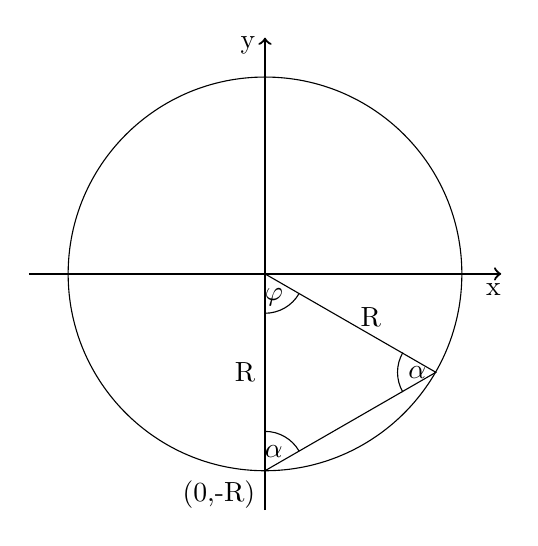
\begin{tikzpicture}[scale=1]
\draw (2.5,0) arc (0:360:2.5);
\draw[->,thick] (-3,0) -- (3,0);
\node[below] at (2.9,0) {x};
\draw[->,thick] (0,-3) -- (0,3);
\node[left] at (0,2.9) {y};
\node[left] at (0,-2.8) {(0,-R)};
\draw (0,-2.5) -- (2.17,-1.25) -- (0,0);
\node[right] at (-0.125,-2.25) {$\alpha$};
\draw (0,-2) arc (90:30:0.5);
\node[left] at (2.17,-1.25) {$\alpha$};
\draw (1.75, -1.5) arc (210:150:0.5);
\node[right] at (-0.125,-0.3) {$\varphi$};
\draw (0,-0.5) arc (270:330:0.5);
\node[left] at (0,-1.25) {R};
\node[right] at (1.09,-0.55) {R};
\end{tikzpicture}
\end{center}
\probend
\bigskip

% S134
\setAuthor{Siim Ainsaar}
\setRound{lõppvoor}
\setYear{2012}
\setNumber{G 5}
\setDifficulty{6}
\setTopic{Kinemaatika}

\prob{Tires}
\solueng
\begin{wrapfigure}{r}{0.4\textwidth}
\includegraphics[width=\linewidth]{2012-v3g-05-r_joonis}
\end{wrapfigure}
The tires have to be turned to a direction that coincides with their movement direction. The car’s rotation axis is probably located on the same line as the axes of the rear wheels. On the other hand in the optimal case it would also be located on both the right and left front wheel’s axis. Therefore the desired angle
\[
\beta =
\operatorname{arccot} \left( \frac{a \cot\alpha - b}{a} \right)
=
\operatorname{arccot} \left( \cot\alpha - \frac ba \right).
\]
\probend
\bigskip

% S135
\setAuthor{Jaan Kalda}
\setRound{lõppvoor}
\setYear{2014}
\setNumber{G 5}
\setDifficulty{6}
\setTopic{Kinemaatika}

\prob{Combs}
\solueng
If the grey comb moves by one teeth then the new figure is identical to the initial one and therefore the dark spot has moved by one “wavelength”. For one “wavelength” of the spots there are 7 “wavelengths” of the grey comb’s teeth, therefore the grey spots move 7 times faster than the grey comb: $v=\SI 7{cm/s}$.
\probend
\bigskip

% S136
\setAuthor{Mihkel Kree}
\setRound{lahtine}
\setYear{2014}
\setNumber{G 10}
\setDifficulty{8}
\setTopic{Kinemaatika}

\prob{Rotation of the Sun}
\solueng
Let the speed of the Sun on the equator be $v$. Because the points A and B approach us and withdraw from us with the velocity $v$ then the measured wavelengths $\lambda_\text{A}$ and $\lambda_\text{B}$ differ from the initial wavelength $\lambda_0$ due to the Doppler shift. The shorter wavelength $\lambda_\text{A}=\lambda_0(1-v/c)$ seems to be radiated from the point A and the longer $\lambda_\text{B}=\lambda_0(1+v/c)$ from the point B.\\
If you do not know the Doppler formula by heart then you can discuss as follows. Let the radiation source move towards us with a velocity $v$. The frequency of the wave corresponding to the wavelength $\lambda_0$ is $f_0=\frac{c}{\lambda_0}$, therefore we can think that the wave crest is radiated after each interval $\tau = 1/f_0 = \lambda_0/c$ that corresponds to the wave’s period. Let the first wave crest be radiated at some moment. During one period it moves to a distance $x=c\tau$; the source itself, however, moves towards us by $\Delta x = v\tau$ during this time and radiates the next crest from there. So, it seems to us as the observer that the distance between two crests (or the wavelength) is $\lambda'=x-\Delta x=(c-v)\tau = \lambda_0(1-v/c)$.\\
The difference of wavelengths measured from the points A and B is expressed therefore as
\[
\Delta\lambda = \lambda_\text{B}-\lambda_\text{A} = 2\lambda_0 v/c,
\]
where we can easily express the speed $v=c\Delta\lambda/2\lambda_0$ and with this the rotation period as well:
\[
T_\text{p}=\frac{2\pi r}{v}=\frac{4 \pi r \lambda_0}{c\Delta \lambda}=
\frac{4 \cdot 3.14 \cdot 7\cdot 10^8 \cdot 5.9 \cdot 10^{-7}}{3\cdot 10^8\cdot 7.8\cdot 10^{-12}}\,\text{s}\approx 26T_\mathrm{m}.
\]
The Sun is not a solid object, its different latitudes rotate with different angular velocities. In the regions close to poles it takes approximately 34 days to make one full turn.
\probend
\bigskip

% S137
\setAuthor{Jaan Kalda}
\setRound{lõppvoor}
\setYear{2014}
\setNumber{G 9}
\setDifficulty{8}
\setTopic{Kinemaatika}

\prob{Wire rings}
\solueng
Let us go to a frame of reference that rotates with an angular velocity $\omega/2$; there it can be seen that the intersection point does not rotate but moves radially. Therefore in a laboratory frame of reference its angular velocity is $\omega/2$; the chord $AB$ rotates with this angular velocity; since a central angle is double an inscribed angle then the radius $OB$ (where $O$ is the center of the still ring) rotates with the angular velocity $\omega$ and therefore the velocity of the intersection point is similarly equal to $\omega R$.
\probend
\bigskip

% S138
\setAuthor{Jaan Kalda}
\setRound{lahtine}
\setYear{2016}
\setNumber{G 9}
\setDifficulty{9}
\setTopic{Kinemaatika}

\prob{Anemometer}
\solueng
The relative differences of the propagation times are small, therefore we can assume that the speed of sound is considerably bigger from the speed of wind. Let us observe the travel of sound in the wind’s frame of reference where $x$- and $y$-directional components ($s_x=u_x\frac a{c_s}$ and $s_y=u_y\frac a{c_s}$) of the relative displacement of the sensors are also small: $s_x, s_y\ll a$; $u_x$ and $u_y$ mark the components of the wind’s velocity and $c_s$ – the speed of light. Strictly saying the exact flight times $t_A$, $t_B$ and $t_C$ should have been in this equation but the displacements themselves are small and due to the small differences of the propagation times each error is already insignificantly small. Therefore we get the following equations for the propagation times:
\begin{align*}
t_A&=\frac 1{c_s}\left(a+u_y\frac a{c_s}\right),\\
t_B&=\frac 1{c_s}\left(a+u_x\frac a{c_s}\right)\;\; \mbox{and}\\
t_C&=\frac 1{c_s}\left(a-u_x\frac a{c_s}\right),
\end{align*}
where $ \frac a{c_s}=\frac 12(t_B+t_C)$,
$$u_x=\frac {c_s^2}a\left[t_B-\frac 12(t_B+t_C)\right]=c_s\frac{t_B-t_C}{t_B+t_C}=2a\frac{t_B-t_C}{(t_B+t_C)^2}\approx \SI{6.1}{m/s}$$
and
$$u_y=\frac {c_s^2}a\left[t_A-\frac 12(t_B+t_C)\right]=2a\frac{2t_A-t_B-t_C}{(t_B+t_C)^2}\approx \SI{7.1}{m/s}.$$
Therefore the speed of the wind $u=\sqrt{u_x^2+u_y^2}\approx \SI{9.4}{m/s}$.
\probend
\bigskip

% S139
\setAuthor{Jaan Kalda}
\setRound{lõppvoor}
\setYear{2016}
\setNumber{G 9}
\setDifficulty{9}
\setTopic{Kinemaatika}

\prob{Motorboat}
\solueng
Let us observe the movement of the motorboat with respect to air: initially $l_1=t_1v_1=\SI{2700}m$ to East, then $l_2=t_2v_2=\SI{900}m$ to South-East and finally $l_3=t_3v_3=\SI{450}m$ to South-West. Altogether the displacement towards South was $L_S=\frac{l_2+l_3}{\sqrt 2}\approx \SI{955}m$ and towards East $L_E=l_1+\frac{l_2-l_3}{\sqrt 2}\approx \SI{3018}m$, with respect to ground, however, the displacement was towards South by $l$. Therefore the air had to move by $L_E$ towards West and by $l-L_S$ towards South. From this we get the speed of the wind to be
$$v_t=\frac{\sqrt{L_S^2+(l-L_S)^2}}{t_1+t_2+t_3}\approx \SI{11.9}{m/s}\approx \SI{12}{m/s}.$$
\probend
\bigskip

% S140
\setAuthor{Kristian Kuppart}
\setRound{lahtine}
\setYear{2013}
\setNumber{G 2}
\setDifficulty{3}
\setTopic{Magnetism}

\prob{Magnet mirror}
\solueng
After getting into the magnetic field the particle starts to move along a circle. We can find its radius by observing that the centripetal force needed for circular movement is caused by the Lorentz force:
\[m\frac{v^2}{r}=qvB, \quad \text{millest} \quad r=\frac{mv}{qB}.\]
If the falling angle $\alpha$ is small enough the particle goes through the magnetic field strip. If we start to increase $\alpha$ a situation occurs where by one moment the particle does not go through the magnetic field strip but “reflects” back. In this limit case (see figure):
\[r\sin\alpha_\text{max}+d=r, \quad \text{from which} \quad \alpha_\text{max}=\sin^{-1}\left(1-\frac{d}{r}\right).\]
\begin{center}
\includegraphics[width=0.9\textwidth]{2013-lahg-02-magPeegLah}
\end{center}
\probend
\bigskip

% S141
\setAuthor{Andreas Valdmann}
\setRound{lahtine}
\setYear{2013}
\setNumber{G 5}
\setDifficulty{4}
\setTopic{Magnetism}

\prob{Generator}
\solueng
a) The electric current in the generator’s winding (in the wire contour) occurs due to an electromagnetic induction and this process is described by the Faraday’s law
$$
\varepsilon = -\frac{\Delta\Phi}{\Delta t},
$$
where $\varepsilon$ is the electromotive force in volts and $\Delta\Phi$ is the change of magnetic flux going through the wire contour during the time $\Delta t$. The value of the magnetic flux $\Phi$ depends on the winding position with respect to the generator’s magnets. By increasing the winding’s rotation frequency by two times it takes two times less time to change the magnetic flux $\Delta\Phi$ and due to that the electromotive force increases by two times. Because there are no losses in the generator then its internal resistance can be assumed to be zero and in the given case the generator’s terminal voltage $U$ is always is equal to its electromotive force. The power dissipated by the lamp is expressed as 
$$
P = UI = \frac{U^2}{R},
$$
where $I$ is the current in the lamp and $R$ is the lamp’s resistance. If the latter does not change then the power increases consequently by $2^2=4$ times when the voltage is increased by two times. Therefore $P_1=4P_0$.\\
b) To get a better picture of the torque’s expression let us imagine that the generator is turned by a crank that has an arm length $l$ and where there is a tangential force $F$ applied to its end. Torque $M$ is expressed as $M=Fl$. Since there are no losses the power of the generator’s turning is equal to the power dissipated by the lamp. From the definition we know that mechanical power is the rate of doing work, meaning
$$
P = \frac{A}{\Delta t},
$$
where $A$ is the work done during the time $\Delta t$ which is in turn expressed as the product of force and displacement $A=F \Delta s$. The displacement $\Delta s$ in this case is the tangential movement of the crank’s end during the time $\Delta t$. The displacement of the crank’s end is expressed as $\Delta s=\Delta\phi l$ where $\Delta\phi$ is the turning angle corresponding to the displacement. So, we can express the mechanical power:
$$
P = F \frac{\Delta s}{\Delta t} =Fl \frac{\Delta\phi}{\Delta t}.
$$
Let us notice that the $\Delta\phi / \Delta t$ in the equation is the angular velocity $\omega$ of the crank’s turning. Equating the result with the torque expression found earlier we get the simple relation $P=M\omega$. In the initial case the torque turning the generator was therefore $M_0 = P_0/\omega_0$. Because $\omega_1=2\omega_0$ and $P_1=4P_0$ then after changing the frequency the torque was $M_1 = P_1/\omega_1=2P_0/\omega_0$.
\probend
\bigskip

% S142
\setAuthor{Eero Vaher}
\setRound{lahtine}
\setYear{2013}
\setNumber{G 6}
\setDifficulty{5}
\setTopic{Magnetism}

\prob{Revolving ball}
\solueng
Let the charge of the positively charged ball be $Q$. In the described magnetic field the ball would be affected by a Lorentz force $F_L=QvB$. This force would be the centripetal force $F_k=\frac{mv^2}{r}$ applied to the ball. We get $QvB=\frac{mv^2}{r}$. Two isolated balls with equal masses rotate around a common center of mass, therefore the distance between them is $d=2r$. The centripetal force holding the balls in the circular orbit is a coulombic force of value $F_C=\frac{kqQ}{d^2}=\frac{kqQ}{4r^2}$. Because the charges rotating around each other have to have the opposite signs then $|F_C|=-F_C$. Equating the centripetal force and coulombic force we get $\frac{mv^2}{r}=-\frac{kqQ}{4r^2}$, meaning $QvB=-\frac{kqQ}{4r^2}$. As the final result we get $q=-\frac{4vBr^2}{k}$.
\probend
\bigskip

% S143
\setAuthor{Kristian Kuppart}
\setRound{piirkonnavoor}
\setYear{2018}
\setNumber{G 10}
\setDifficulty{6}
\setTopic{Magnetism}

\prob{Cyclotron}
\solueng
In the cyclotron the particles start to move clock-wise along a circle with a continuously increasing half circles. The radius of a particle is expressed as $r=mv/qB$ where $v$ is the particle’s velocity. The particle leaves the cyclotron when its trajectory radius gets as big as the cyclotron’s radius $R$, in this case its velocity is $v=qBR/m$. During one full circle the particle gets a kinetic energy from $\varepsilon_k=2qEd$ the electric field, because the particle goes through the strip two times during this time. Therefore the velocity of the particle when exiting the cyclotron is
\[\frac{mv^2}{2}=2qEdn, \qquad v^2=\frac{4qEdn}{m}.\]
Expressing $n$ from these equations we get $\displaystyle n=\frac{qB^2R^2}{4mEd}$.
\probend
\bigskip

% S144
\setAuthor{Kristian Kuppart}
\setRound{piirkonnavoor}
\setYear{2013}
\setNumber{G 10}
\setDifficulty{7}
\setTopic{Magnetism}

\prob{Mass spectrometer}
\solueng
In the case of potential difference $U$ an accelerated charged particle gets a kinetic energy $\frac{mv^{2}}{2}=qU$, from here we express the velocity of the particle: $v=\sqrt{\frac{2qU}{m}}$. Because the magnetic field is perpendicular to the velocity the charged particle starts to move along a circle when entering the magnetic field, the radius of the circle is $R=\frac{mv}{qB}$. By the time when the particle reaches the detector it has covered half of the circle. Let $m_{2}$ be the mass of the heavier isotope and $m_{1}$ the mass of the lighter isotope. In that case
\[ 
2\left(\frac{m_{1}v_{1}}{qB}-\frac{m_{2}v_{2}}{qB}\right)=d, 
\]
meaning 
\[ 
m_{2}v_{2}=\frac{qBd}{2}+m_{1}v_{1 }.
\]
Considering that $v_{1}=\sqrt{\frac{2eU}{m_{1}}}$ and $v_{2}=\sqrt{\frac{2eU}{m_{2}}}$ where $e$ is the elementary charge we can write the previous equation as 
\[ \sqrt{m_{2}}=\sqrt{m_{1}}+\frac{Bd}{2}\sqrt{\frac{e}{2U}}. \]
Taking into account that $m_{2}=\frac{\mu_{2}}{N_{A}}$ and $m_{1}=\frac{\mu_{1}}{N_{A}}$, where $N_{A}$ is the Avogadro constant, we get:
\[ \mu_{2}=N_{A}\left(\sqrt{\frac{\mu_{1}}{N_{A}}}+\frac{Bd}{2}\sqrt{\frac{e}{2U}}\right)^{2}.\]
\probend
\bigskip

% S145
\setAuthor{Jaan Kalda}
\setRound{piirkonnavoor}
\setYear{2015}
\setNumber{G 9}
\setDifficulty{8}
\setTopic{Magnetism}

\prob{Magnetic field}
\solueng
\begin{center}
\includegraphics[width=0.7\textwidth]{2015-v2g-09-magnetvalilah}
\end{center}
The particle performs a circular movement in the magnetic field, see figure; we find the radius of the ring from the Newton’s second law $Bqv=mv^2/R$ where $R=\frac{mv}{qB}$. Before and after the circular movement the trajectory is a line, moreover the transition into a circle is without a breakpoint, meaning that the lines are the circle’s tangent. For small velocities, if $R<a$, meaning $v<\frac{Bqa}{m}$, then the particle goes straight back, meaning that the exiting angle is $\varphi=\pi \SI{}{rad}=180^\circ$.\\
When exiting the magnetic field the velocity’s vector is perpendicular to the circle’s radius, meaning $\angle OBD=\frac \pi 2$, which is why $\varphi=\angle COB$. Therefore $\varphi=\arcsin \frac{BC}{BO}=\arcsin \frac{a}{R}=\arcsin \frac{qBa}{mv}$.
\probend
\bigskip

% S146
\setAuthor{Eero Vaher}
\setRound{lahtine}
\setYear{2015}
\setNumber{G 10}
\setDifficulty{9}
\setTopic{Magnetism}

\prob{Charged pendulum}
\solueng
The ball is affected by the gravity force $F_g$, thread’s tension $T$ and the Lorentz force $F_L$. The ball stays on the circle’s arc-shaped trajectory until the projections of the forces applied to it that are to the thread’s direction satisfy the equation $T+F_L-F_g\cos\alpha=F_k$ where $\alpha$ is the angle of deflection from the equilibrium position and $F_k$ is the necessary centripetal force to stay on the circle’s arc. The thread cannot be tense when the ball strays away from the circle’s arc-shaped trajectory. Therefore the ball’s trajectory is no longer a circle’s arc when $F_L>F_g\cos\alpha+F_k$. Let $v$ be the ball’s velocity for the angle $\alpha$ which we can find from the conversation of energy $\frac{mv^2}{2}=-mg\Delta h$, where $\Delta h=l\cos\alpha-l+H$ is the ball’s height change. Therefore 
\[
v=\sqrt{2g\left(l\cos\alpha-l+H\right)}=\sqrt{2gl\left(\cos\alpha-\frac{1}{8}\right)}
\]
and the equation needed to be solved is $qBv=mg\cos\alpha+\frac{mv^2}{l}$, meaning
\[
qB\sqrt{2gl\left(\cos\alpha-\frac{1}{8}\right)}=mg\cos\alpha+2mg\left(\cos\alpha-\frac{1}{8}\right).
\]
Squaring both sides we get
\[
2q^2B^2gl\left(\cos\alpha-\frac{1}{8}\right)=m^2g^2\left(3\cos\alpha-\frac{1}{4}\right)^2.
\]
Because $2q^2B^2l=\frac{3}{2}m^2g$ we can express this equation as $\frac{3}{2}\cos\alpha-\frac{3}{16}=9\cos^2\alpha-\frac{3}{2}\cos\alpha+\frac{1}{16}$. We get a quadratic equation $9\cos^2\alpha-3\cos\alpha+\frac{1}{4}=0$, meaning $9\left(\cos\alpha-\frac{1}{6}\right)^2=0$. Because the two solutions of this quadratic equations are equal then either $F_L\leq F_g\cos\alpha+F_k$ or $F_L\geq F_g\cos\alpha+F_k$ for each $\alpha$. Observing the case $\cos\alpha=\frac{1}{8}$ we see that $F_L\leq F_g\cos\alpha+F_k$ and therefore trajectory of the ball is a circle’s arc of radius $l$. The height of the arcs ends from the equilibrium position is $\frac{7}{8}l$.
\probend
\bigskip

% S147
\setAuthor{Jaan Kalda}
\setRound{lõppvoor}
\setYear{2017}
\setNumber{G 10}
\setDifficulty{10}
\setTopic{Magnetism}

\prob{Electrons}
\solueng
To find the maximal $y$-directional diameter we observe the particles that move on $x-y$ plane. In this case the trajectory of the electron is a circle because the force $F=evB$ applied by the magnetic field has a constant value and is always perpendicular to the velocity. We can find the radius if we equate the force applied by the magnetic field to the centripetal force:
$$\frac{mv^2}{R}=evB \hence R = \frac{mv}{Be}.$$
All the electrons in that plane move on a circle with the same radius and we can find the trajectories of the electrons moving at different angles by just turning this circle around the point O. An electron reaches the furthest on the positive direction of the $y$-axis if when hitting the screen it is as far as possible from the origin, meaning it has covered exactly half of a circle’s arc, see figure:
\begin{center}
	\begin{tikzpicture}
	\def\aEl{1};
	\def\rEl{1.5};
	\coordinate (P1) at (-\aEl,{sqrt(4*\rEl*\rEl-\aEl*\aEl)});
	\coordinate (P2) at (-\aEl*0.5,{0.5*sqrt(4*\rEl*\rEl-\aEl*\aEl)});
	\node[label=below right:O, fill=black, circle,inner sep=1pt] at (0,0){};
	\path let \p1=(P1) in node [label=left:b] at (-\aEl, \y1/2){};
	\node[label=right:Q, fill=black, circle,inner sep=1pt] at (P2){};
	\node[label=below:a] at (-\aEl/2,0){};
	\node [label=above:$y$] at (-\aEl, 2.5*\rEl){};
	\draw[->] (-\aEl,-\rEl/2) -- (-\aEl, 2.5*\rEl);
	\draw (0,0) -- (P1);
	\draw (0,0) -- (-\aEl,0);
	%\draw (0,0) arc ({-90+asin(\aEl/(2*\rEl))}:{360-(-90+asin(\aEl/(2*\rEl)))}:\rEl);
	\draw (0,0) arc ({-90+asin(\aEl/(2*\rEl))}:90+asin(\aEl/(2*\rEl)):\rEl);
	%\draw [red](P1) ++ (-90:0.4) arc (-90:-90+\angKatus:0.4);
	\end{tikzpicture}
\end{center}
Because the screen is at the distance $a$ from the source of the electrons then according to the Pythagorean theorem we get the maximal $y$ value of the spot to be 
$$b=\sqrt{4R^2-a^2} = \sqrt{4\left(\frac{mv}{Be}\right)^2-a^2}.$$
From here we see that a smaller diameter corresponds to a smaller $R$ and the maximal $y$-directional diameter is indeed when the particle moves on the $x-y$ plane like we claimed in the beginning.\\
Turning the circle’s arc along the point $O$ we see that for the minimal $y$-directional value the circle is a tangent to the screen, see figure:
\begin{center}
	\begin{tikzpicture}
	\def\aEl{1};
	\def\rEl{1.5};
	\coordinate (P1) at (\rEl-\aEl,{-sqrt(\rEl*\rEl-(\rEl-\aEl)*(\rEl-\aEl))});
	\node[label=above right:O, fill=black, circle,inner sep=1pt] at (0,0){};
	\node[label=below right:Q, fill=black, circle,inner sep=1pt] at (P1){};
	\path let \p1=(P1) in node[label=below:T, fill=black, circle,inner sep=1pt] at (0,\y1){};
	%\path let \p1=(P1) in node [label=left:b] at (-\aEl, \y1/2){};
	\node[label=above:a] at (-\aEl/2,0){};
	\node [label=above:$y$] at (-\aEl, 0.5*\rEl){};
	\draw[->] (-\aEl,-2*\rEl) -- (-\aEl, 0.5*\rEl);
	\draw (0,0) -- (P1);
	\draw (P1) -- ($(P1)-(1.0*\rEl,0)$);
	\draw (0,0) -- (-\aEl,0);
	%\draw (0,0) arc ({180-acos((\rEl-\aEl)/\rEl)}:{360}:\rEl);
	\draw (P1) ++ (-180:\rEl) arc (180:-180:\rEl);
	%\draw (0,0) arc ({180-acos((\rEl-\aEl)/\rEl)}:180:\rEl);
	%\draw [red](P1) ++ (-90:0.4) arc (-90:-90+\angKatus:0.4);
	\end{tikzpicture}
\end{center}
Because the length of the segment QT is $R-a$ then we can find the segment’s CQ $y$-directional component with the Pythagorean theorem
$$y\idx{min}=-\sqrt{R^2-(R-a)^2} = -\sqrt{2aR-a^2}=-\sqrt{\frac{2amv}{Be}-a^2}.$$
Therefore the spot’s $y$-directional diameter is
$$L=\sqrt{\frac{2amv}{Be}-a^2} + \sqrt{4\left(\frac{mv}{Be}\right)^2-a^2}.$$
The brightness is biggest on this spot for the maximal value of $y$ because it corresponds to the electron’s $y$-directional deflection’s $\Delta_y$ extremum. If we mark the electron’s starting angle with $\alpha$ then 
$$\frac{\D \Delta_y}{\D \alpha}=0,$$
meaning in a small starting angle’s interval $\Delta\alpha$ all the electrons arrive to almost exactly the same destination point.\\
Let us find the $z$-directional diameter in the plane $y=0$. The particles that reach the furthest on the $z$-axis have a helical trajectory touching the plane $x=-a$ (from the “top view” of the $x-y$ plane a circle-shaped trajectory of radius $r=\frac a2$ touches the line $x=-a$) and start from the $y-z$ plane, meaning with an initial velocity which has a $x$-projection of $v_x=0$. Next we find
$$\frac a2=\frac {mv_y}{Be}\hence v_y=\frac{aBe}{2m}\hence v_z=\sqrt{v^2-\left(\frac{aBe}{2m}\right)^2}.$$
An electron with this initial velocity travels for half the cyclotron’s period. We can find the period from the relation $T=\frac{2\pi R}{v} = \frac{2\pi m}{Be}$. A half period is therefore $t=\frac{T}{2}=\frac{\pi m}{Be}$ and we get the spot’s $z$-directional dimension to be 
$$2\cdot tv_z=\pi\sqrt{\left(\frac{2mv}{Be}\right)^2-a^2}.$$
\probend
\bigskip

% S148
\setAuthor{Taavi Pungas}
\setRound{piirkonnavoor}
\setYear{2014}
\setNumber{G 6}
\setDifficulty{4}
\setTopic{Staatika}

\prob{Ring}
\solueng
For the system to be in equilibrium the nut has to be located exactly below the rope’s attachment point. Secondly: in the case of the nut’s maximal height the circle’s angle of inclination in the nut’s location is $\alpha$, where $\tan \alpha = \mu$ – then the nut is exactly on the verge of slipping. In this case the angle between the radius drawn up to the nut and the vertical is also $\alpha$. From the formed triangle we see that $h=L+2R\cos \alpha = L+ \frac{2R}{\sqrt{1+\mu^2}}$.
\probend
\bigskip

% S149
\setAuthor{Mihkel Rähn}
\setRound{piirkonnavoor}
\setYear{2015}
\setNumber{G 7}
\setDifficulty{5}
\setTopic{Staatika}

\prob{Bolt cutter}
\solueng
The force transmission is based on the principle of moments where the torque with respect to the turning axis by total is equal to zero. For the handle
\[ \SI{600}{mm}\cdot\SI{90}{N}-\SI{100}{mm}\cdot F_k = 0 \quad\Rightarrow\quad F_k = \SI{540}{N}, \]
where $F_k$ is the force applied to the blade by the handle. Similarly for the blades
\[ \SI{160}{mm}\cdot F_k - \SI{80}{mm}\cdot F_l = 0 \quad\Rightarrow\quad F_l = 2F_k, \]
where $F_l$ is the force applied to the bolt by the cutter.\\
From these equation we can find the force $F_l$ applied to the blades
\[ F_l = \SI{1080}{N}.\]
\probend
\bigskip

% S150
\setAuthor{Mihkel Rähn}
\setRound{piirkonnavoor}
\setYear{2014}
\setNumber{G 7}
\setDifficulty{6}
\setTopic{Staatika}

\prob{Block}
\solueng
The upper block does not slide if the force caused by the acceleration does not exceed the static friction. For the upper block we can express the maximal velocity when the block does not yet slide from the Newton’s second law $a_2=\mu_2g$. If the upper block does not slide then the two blocks can be treated as one body. The Newton’s second law for the block system is $(m_1+m_2)a_{12} = -\mu_1 (m_1+m_2)g+F$. In the limit case the accelerations $a_{12}$ and $a_2$ are equal. Replacing the previously found acceleration $a_2$ to the equation as $a_{12}$ we get $F=(m_1+m_2)(\mu_1+\mu_2)g$.\\
The problem can also be solved by writing the Newton’s second law for the bottom block, while taking both frictions into account.
\probend
\bigskip

% S151
\setAuthor{Mihkel Rähn}
\setRound{lõppvoor}
\setYear{2014}
\setNumber{G 6}
\setDifficulty{6}
\setTopic{Staatika}

\prob{Polyspast}
\solueng
For a frictionless block the tension in the main rope is constant, only its direction changes. In the case of a block with friction a part of the main rope’s tension is transmitted to the block, moreover in the first approximation downwards and upwards directed frictions compensate each other. To satisfy the equilibrium condition the block’s attachment tension has to be equal to sum of the main rope’s tensions that go through the block. In the case of non-sliding knots the upwards and downwards directed tensions have to be in balance. It is easy to start solving if you assume the force from the rescuer’s side to be $F$ and begin by going through the polyspast from the rescuer’s end. In the frictionless case the force transmission is $\frac{5}{1}$ and in the case of friction $\frac{2,4}{1}$. 
\begin{center}
\includegraphics[scale=0.25]{2014-v3g-06-PolyspastL1}
\includegraphics[scale=0.25]{2014-v3g-06-PolyspastL2}
\end{center}
\probend
\bigskip

% S152
\setAuthor{Andreas Valdmann}
\setRound{piirkonnavoor}
\setYear{2018}
\setNumber{G 9}
\setDifficulty{6}
\setTopic{Staatika}

\prob{Sledge}
\solueng
Firstly we see that if Juku pulled the rope of the sledge horizontally then no matter how big the pulling force is the sledge would not start moving because the friction applied to Juku is smaller from the force that is needed for the sledge to start moving:
\[
\mu_1 m_1 g < \mu_2 m_2 g.
\]
Juku’s soles are actually the first to start moving.\\
If Juku pulls the rope at a certain angle upwards then a vertical force component $F_{\mathrm{v}}$ is created in the rope, this force pulls the sledge upwards and presses Juku downwards. Therefore on the verge of sliding Juku is affected by a friction $F_{\mathrm{h}1} = \mu_1 \left(m_1 g + F_{\mathrm{v}}\right)$ and the sledge is affected by a friction $F_{\mathrm{h}2} = \mu_2 \left(m_2 g - F_{\mathrm{v}}\right)$ when it is on the verge of sliding. Because the minimal angle was asked then the sledge has to have barely exceeded the sliding limit and Juku has to barely stay below it, meaning in the limit case $F_{\mathrm{h}1} = F_{\mathrm{h}2} = F_{\mathrm{h}}$ where $F_{\mathrm{h}}$ marks the horizontal component of the force occurring in the rope. From the force balance equation
\begin{equation*}
\mu_1 \left(m_1 g + F_{\mathrm{v}}\right) = \mu_2 \left(m_2 g - F_{\mathrm{v}}\right)
\end{equation*}
we can express the vertical component of the force occurring in the rope:
\begin{equation*}
\mu_1 m_1 g + \mu_1 F_{\mathrm{v}} = \mu_2 m_2 g - \mu_2 F_{\mathrm{v}},
\end{equation*}
\begin{equation*}
F_{\mathrm{v}} \left(\mu_1 + \mu_2\right) = g\left(\mu_2 m_2 - \mu_1 m_1\right),
\end{equation*}
\begin{equation*}
F_{\mathrm{v}} = g\frac{\mu_2 m_2 - \mu_1 m_1}{\mu_1 + \mu_2}.
\end{equation*}
To find the force’s horizontal component we can replace the gotten result in the equation of the friction applied to Juku
\begin{equation*}
F_{\mathrm{h}} = \mu_1 \left(m_1 g + g\frac{\mu_2 m_2 - \mu_1 m_1}{\mu_1 + \mu_2}\right)
\end{equation*}
and express
\begin{align*}
F_{\mathrm{h}} &= g \mu_1 \frac{m_1 \left(\mu_1 + \mu_2\right) + \mu_2 m_2 - \mu_1 m_1}{\mu_1 + \mu_2} = \\
&= g \mu_1 \frac{\mu_2 m_1 + \mu_2 m_2}{\mu_1 + \mu_2} = g\mu_1\mu_2\frac{m_1+m_2}{\mu_1+\mu_2}.
\end{align*}
The angle between the sledge’s rope and the ground is
\begin{equation*}
\alpha = \arctan\left(\frac{F_{\mathrm{v}}}{F_{\mathrm{h}}}\right) = \arctan\left(\frac{\mu_2 m_2 - \mu_1 m_1}{\mu_1 \mu_2 \left(m_1 + m_2\right)}\right) = \ang{21}.
\end{equation*}
\probend
\bigskip

% S153
\setAuthor{Mihkel Kree}
\setRound{lahtine}
\setYear{2013}
\setNumber{G 8}
\setDifficulty{7}
\setTopic{Staatika}

\prob{Thread roll}
\solueng
Let us observe the balance of the torques applied to the cylinder with respect to the axis that goes through the support point. The vectors of the surface’s normal force and friction go through the support point which is why they do not create a torque. A torque is created by two forces: the gravity force $mg$ applied to the cylinder’s center and the thread’s pulling force $F$. Calculating the gravity force’s arm from a simple triangle we get the torque to be $\tau=mgr\sin\alpha$. In the case of equilibrium the pulling force $F$ creates a torque $-\tau$ that is as big but has the opposite direction. The minimal force has to correspond to the maximal force arm. Let us make sure that if the force $F$ was applied to a point diametrically opposite to the support point then we get the maximal arm $2r$ that has a corresponding minimal pulling force
\[F\idx{min}=\frac{\tau}{2r}=\frac{mg\sin\alpha}{2}.\]
\probend
\bigskip

% S154
\setAuthor{Andres Põldaru}
\setRound{lahtine}
\setYear{2014}
\setNumber{G 8}
\setDifficulty{7}
\setTopic{Staatika}

\prob{Cyclist}
\solueng
Because the rear wheel is about to rise into the air then no forces are applied to it. The only forces applied to the bicycle are the gravity force and the force at the contact point of the front wheel and the ground. Because the bicycle is moving with an even velocity and does not start to rotate or fall down the sum of the forces applied to the system consisting of the bicycle and the cyclist has to be zero and the torque with respect to each point has to be zero as well. The value and direction of the gravity force is known. The second force has to be as big and has to have the opposite direction to balance the gravity force. In addition the forces have to be located on the same line so that the bicycle with the cyclist would not start to rotate. Therefore the center of mass has to be above the contact point of the front wheel and the ground and the sum of the friction and normal force is vertical. From simple geometry we get $\alpha=\arctan(\frac{d}{2h})$ and $\mu\ge\frac{d}{2h}$. 
\begin{center}
\includegraphics[width=0.6\textwidth]{2014-lahg-08-ratas}
\end{center}
\probend
\bigskip

% S155
\setAuthor{Stanislav Zavjalov}
\setRound{lahtine}
\setYear{2012}
\setNumber{G 9}
\setDifficulty{9}
\setTopic{Staatika}

\prob{Rope in groove}
\solueng
Let the rope’s mass be $m$. Let us observe the rope’s right side. The vertical component of the rope’s tension $T \sin \theta$ at the contact point of the rope and the plate has to balance the weight of the rope hanging in the air, $\frac{f}{2}mg$. Now let us observe the part lying on the plate, its mass is $\frac{1-f}{2}m$. Therefore both the normal force and the maximal friction (because $\mu = 1$) are $\frac{1-f}{2}mg \cos \theta$. The friction has to balance the component of the gravity force along the rope, $\frac{1-f}{2}mg \sin \theta$, and the tension $T=\frac{f m g}{2 \sin \theta}$. 
$$\frac{f m g}{2 \sin \theta} + \frac{1-f}{2}mg \sin \theta = \frac{1-f}{2}mg \cos \theta.$$
From here we can express the answer
$$f = \frac{1-\tan \theta}{1+\tan \theta} \tan \theta. $$
\probend
\bigskip

% S156
\setAuthor{Jaan Kalda}
\setRound{lõppvoor}
\setYear{2017}
\setNumber{G 9}
\setDifficulty{9}
\setTopic{Staatika}

\prob{Roof}
\solueng
At the contact point $A$ of the two wires (see figure below) the wires affect each other with forces of opposite directions due to symmetry and the Newton’s third law; at the contact point $B$ of the wire and cylinder the wire is affected by a normal force that is perpendicular to the wire and because of this the extension of that force goes through the axis $Q$ of the cylinder. The gravity force is applied to the center $C$ of the wire. Since the wire is in balance and the forces are applied to it at three points then the extensions of these forces have to intersect at one point $O$ (otherwise a third force would affect the wire with respect to the intersection point of two forces with a torque different from zero and the wire would start to move). So, the horizontal drawn from the point $A$, the vertical drawn from the point $C$ and the extension of the line $QB$ all have to intersect at one point. Let us notice that $\angle ACO=\alpha/2$ and $\angle AOB=\alpha/2$, which is why
$$|AO|=|AC|\sin(\alpha/2)=(L/2)\sin(\alpha/2),$$
$$|AB|=|AO|\sin(\alpha/2)=(L/2)\sin^2(\alpha/2)$$
and
$$R=|QB|=|AB|\tan(\alpha/2)=(L/2)\sin^3(\alpha/2)/\cos(\alpha/2).$$
\begin{center}
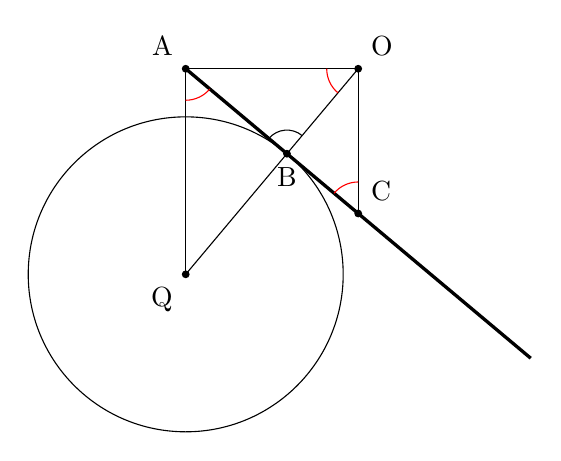
\begin{tikzpicture}
\usetikzlibrary{calc}
\def\angKatus{50};
\def\rKatus{2};
\coordinate (P1) at (0,{\rKatus/sin(\angKatus)});
\coordinate (P2) at ({\rKatus/sin(\angKatus)/tan(\angKatus)},{\rKatus/sin(\angKatus)});
\coordinate (P3) at ({\rKatus/sin(\angKatus)/tan(\angKatus)},{\rKatus/sin(\angKatus)-\rKatus/sin(\angKatus)/tan(\angKatus)/tan(\angKatus)});
%\fill (0,0) circle (0.05);
\node [label=below left:Q, fill=black, circle,inner sep=1pt] at (0,0){};
\draw (0,0) circle (\rKatus);
\node [label=above left:A, fill=black, circle,inner sep=1pt] at (P1){};
\node [label=above right:O, fill=black, circle,inner sep=1pt] at (P2){};
\node [label=above right:C, fill=black, circle,inner sep=1pt] at (P3){};
\node [label=below:B, fill=black, circle,inner sep=1pt] at (\angKatus:\rKatus){};
\draw [very thick](P1) -- (P3) -- ++($(P3)-(P1)$);
\draw (0,0) -- (P2);
\draw (0,0) -- (P1);
\draw (P1) -- (P2);
\draw (P3) -- (P2);
\draw [red](P1) ++ (-90:0.4) arc (-90:-90+\angKatus:0.4);
\draw [red](P3) ++ (90:0.4) arc (90:90+\angKatus:0.4);
\draw [red](P2) ++ (180:0.4) arc (180:180+\angKatus:0.4);
\draw (\angKatus:\rKatus) ++ (\angKatus:0.3) arc (\angKatus:90+\angKatus:0.3);
\end{tikzpicture}
\end{center}

Analyzing the stability we notice that if the “roof” would rotate as a whole then the center of mass moves along a circle and the only question would be if it is higher or lower than the cylinder’s axis $Q$; in the latter case the center of mass would be in the lowest location in the initial position and the system is stable. Therefore the stability condition is

$$|AQ|<|AC|\cos(\alpha/2).$$

If we replace this into the equation

$$|AQ|=|AB|/\cos(\alpha/2)=(L/2)\sin^2(\alpha/2)/\cos(\alpha/2)$$

and 

$$|AC|\cos(\alpha/2)=(L/2)\cos(\alpha/2),$$

then we get that $\sin^2(\alpha /2) < \cos ^2(\alpha /2)$. Because in the case of the roof $0<\frac{\alpha}{2}<90$ must apply then both sin and cos are positive and we can take a square root from both sides. We get the condition $\cos$ that applies when $\alpha<\pi/2$. Let us notice that the last condition can be presented in different ways using the relation between $R$, $L$ and $\alpha$.
\probend
\bigskip

% S157
\setAuthor{Jaan Kalda}
\setRound{lõppvoor}
\setYear{2015}
\setNumber{G 9}
\setDifficulty{10}
\setTopic{Staatika}

\prob{Dumbbell with a thread}
\solueng
Three forces are applied to the rod. Due to the torque balance the extensions of these forces have to intersect at one point, let this point be $C$. Let the thread’s application point be $N$ and the ends of the rod $A$ and $B$, see figure. Because the rod is rotating around the block $A$ before it starts to shift then the point’s $B$ velocity vector is perpendicular to $AB$ and the friction’s vector is applied to the point $B$; because of this $\angle ABC=\frac{\pi}{2}$. Because at the moment of the displacement’s start the frictions are equal then the force triangle $\vec F_1+\vec F_2=\vec T$ is an isosceles triangle, therefore the similar triangle $CBE$ of the force triangle is also an isosceles triangle (the line $BE$ is drawn in parallel to $\vec T$ and $E$ is located on the extension of $\vec F_1$, see figure). Let $|CB|=b$; then also $|CE|=b$. Then due to the similarity of the triangles $ANC$ and $ABE$ we can see that $|AC|=3b$. From the Pythagorean theorem for the triangle $ABC$ we get $9b^2=b^2+16a^2$, meaning $b=\sqrt 2a$. Because of this the desired angle $\angle BNC=\arctan \frac ba =\arctan \sqrt 2\approx\SI{0.96}{rad}\approx 55^\circ$
\begin{center}
\includegraphics[width=0.7\textwidth]{2015-v3g-09-pulk_lah}
\end{center}
\probend
\bigskip

% S158
\setAuthor{Eero Vaher}
\setRound{piirkonnavoor}
\setYear{2014}
\setNumber{G 3}
\setDifficulty{2}
\setTopic{Taevamehaanika}

\prob{Rotation period of Earth}
\solueng
The apparent movement of the Sun in the sky is caused both by the Earth’s rotation and orbiting. Due to the Earth’s orbiting the number of Earth’s full turns per year is different by one from the number of average days. Because the direction of the Earth’s orbiting coincides with the direction of the Earth’s rotation the Earth does one additional full turn during a year. Therefore the period of the Earth’s rotation is $P=\frac{365,256}{366,256} \cdot \SI{86400}{\second}=\SI{86164}{\second}$, or $P=\SI{23}{\hour}$.\\

\emph{Alternative solution}\\
The Sun does a full rotation in the sky with the frequency $f_k=\frac{1}{\SI{86400}{\second}}$. The frequency of the Earth’s orbiting is $f_t=\frac{1}{365,256\cdot86400\text{s}}$. Because the direction of the Earth’s orbiting coincides with the direction of the Earth’s rotation the equation $f_k=f_p-f_t$ applies where $f_p$ is the frequency of the Earth’s rotation. From here we can express the period of the Earth’s rotation $P=\frac{1}{f_p}=\frac{1}{f_k+f_t}=\SI{86164}{\second}$ meaning $P=\SI{23}{\hour} \SI{56}{\min} \SI{4}{s}$. \\

\emph{Notes}\\
\begin{itemize}
\item The name “average day” is due to the fact that because of the Earth elliptic orbit the Sun’s apparent angular velocity is a bit variable in the sky.
\item The period of the Earth’s orbiting is also called the sidereal year.
\item In most cases a year is seen as the tropical year not the sidereal year. The tropical year is defined by the recurrence of the equinoxes. The difference between the tropical and sidereal year is caused by the precession of the Earth’s axis. In daily life the Earth’s orbiting or rotation are not important but the Sun’s daily movement in the sky and the repetition of the seasons are. This is why the widely used definitions of the day and year differ from the Earth’s rotation and orbiting periods.
\end{itemize}
\probend
\bigskip

% S159
\setAuthor{Mihkel Pajusalu}
\setRound{lahtine}
\setYear{2014}
\setNumber{G 3}
\setDifficulty{3}
\setTopic{Taevamehaanika}

\prob{Orbit}
\solueng
In this problem we use the approximation that the point mass Moon with a small mass (let it be $m$) orbits around the big point mass Earth. Let us notice that the sum of the gravitational potential energy and kinetic energy of the Moon is constant. 
$$
\frac{mv_1^2}{2}-G\frac{Mm}{r_1}=\frac{mv_2^2}{2}-G\frac{Mm}{r_2}.
$$
In addition the moving bodies on all the orbits have a constant angular momentum. Because the orbits are elliptical then on the furthest and closest distance from the Earth the orbital velocity of the Moon is perpendicular to the line that connects the Moon to the Earth. Therefore the conservation of angular momentum for the furthest and closest distance can be written down as
$$
mv_1r_1=mv_2r_2.
$$
The Moon’s mass cancels out from both of the conservations. We get the system
$$
\begin{array}{c} 
\frac{v_1^2}{2}-G\frac{M}{r_1}=\frac{v_2^2}{2}-G\frac{M}{r_2}.\\
v_1r_1=v_2r_2.
\end{array}
$$
The solutions of the systems $r_2=r_1$, they do not correspond to an elliptic orbit, and
$$r_2=\frac{1}{\frac{2GM}{r_1^2v_1^2}-\frac{1}{r_1}}\approx\SI{430000}{km}.$$
\probend
\bigskip

% S160
\setAuthor{Eero Vaher}
\setRound{piirkonnavoor}
\setYear{2013}
\setNumber{G 6}
\setDifficulty{4}
\setTopic{Taevamehaanika}

\prob{Density of the Sun}
\solueng
The Sun’s radius is $r=\frac{R\sin\alpha}{2}$ and volume $V=\frac{4\pi r^3}{3}$. The Earth’s speed on its orbit around the Sun is $v=\frac{2\pi R}{T}$. For the Earth to stay on its orbit a centripetal force $F=\frac{mv^2}{R}$ has to be applied to it where $m$ is the Earth’s mass. This centripetal force is the gravity force $G\frac{mM}{R^2}$ between the Earth and the Sun where $M$ is the Sun’s mass, therefore $\frac{mv^2}{R}=G\frac{mM}{R^2}$. We get $M=\frac{Rv^2}{G}$. The Sun’s density is expressed from the relation $\varrho=\frac{M}{V}$. 
$$\varrho=\frac{Rv^2}{G} \frac{3}{4\pi r^3}=\frac{24 \pi R^3}{G T^2 \sin^3 \alpha}=\SI{1,4e3}{kg/m^3}.$$
\probend
\bigskip

% S161
\setAuthor{Eero Vaher}
\setRound{piirkonnavoor}
\setYear{2018}
\setNumber{G 6}
\setDifficulty{4}
\setTopic{Taevamehaanika}

\prob{Connected satellites}
\solueng
Without a cable the centripetal force applied to a satellite has to be equal to the gravity force applied to it. For the first satellite $\frac{{mv'_1}^2}{R_1}=G\frac{Mm}{R_1^2}$ where we conclude that $v'_1=\sqrt{\frac{GM}{R_1}}$ and analogically $v'_2=\sqrt{\frac{GM}{R_2}}$.\\
Because the satellites are connected with a cable then the centripetal force applied to the inner satellite has to be the difference between the gravity force applied to it and the cable’s tension. The centripetal force applied to the outer satellite has to be the sum of the gravity force applied to it and the cable’s tension. Therefore
$$\begin{cases}
\frac{mv_1^2}{R_1}=G\frac{Mm}{R_1^2}-T,\\
\frac{mv_2^2}{R_2}=G\frac{Mm}{R_2^2}+T.
\end{cases}$$
Because $v_1=\frac{2\pi R_1}{P}$ and $v_2=\frac{2\pi R_2}{P}$ we can write 
$$\frac{4\pi^2}{P^2}\left(R_1+R_2\right)=GM\frac{R_2^2+R_1^2}{R_1^2R_2^2}.$$
Making the replacement $R_2=2R_1$ we get $\frac{2\pi R_1}{P}=\sqrt{\frac{5GM}{12R_1}}$ and from the replacement $R_1=\frac{R_2}{2}$ it concludes that $\frac{2\pi R_2}{P}=\sqrt{\frac{10GM}{3R_2}}$. The inner satellite orbits due to the cable with a $\sqrt{\frac{12}{5}}$ times smaller speed and the outer with a $\sqrt{\frac{10}{3}}$ times bigger speed.
\probend
\bigskip

% S162
\setAuthor{Eero Vaher}
\setRound{lõppvoor}
\setYear{2013}
\setNumber{G 5}
\setDifficulty{5}
\setTopic{Taevamehaanika}

\prob{Satellite}
\solueng
The centripetal force applied to the satellite on the orbit is the gravity force applied by the Earth to the satellite. We get 
$$\frac{mv^2}{R}=G\frac{Mm}{R^2},$$
where $m$ is the satellite’s mass and $R$ the orbit’s radius. Because a geostationary satellite does not move with respect to the Earth then its orbiting period also has to be 24 h. We get $v=\frac{2\pi R}{t}$. From these equations we get
$$4\pi^2 R^3=GM \Rightarrow R=\sqrt[3]{\frac{GMt^2}{4\pi^2}}=\SI{42400}{km}.$$
The Earth’s center, the satellite and a random point located on the edge of the Earth region seen from the satellite make up a right triangle. Its hypotenuse is the radius of the satellite’s orbit and one of the legs is the Earth’s radius. We get the angle in the Earth’s center to be $\alpha=\arccos{\frac{r}{R}}$ but because we are interested in the diameter of the region seen from the satellite we have to find the angle $2\alpha$. The length of the arc on the Earth’s surface that corresponds to this angle is $d=2r\alpha$ (if the angle is in radians). For the final answer we get
$$d=2r\arccos \left(\frac{r}{\sqrt[3]{\frac{GMt^2}{4\pi^2}}}\right) =\SI{18000}{km}.$$
\probend
\bigskip

% S163
\setAuthor{Jaak Kikas}
\setRound{lahtine}
\setYear{2012}
\setNumber{G 1}
\setDifficulty{1}
\setTopic{Termodünaamika}

\prob{Freezing of water}
\solueng
The dissipated heat $m\idx{water} \lambda$ from the freezing of water has to exactly go to the heating of water: $m\idx{water} \lambda = c\idx{ice} m\idx{ice} (t - t_0)$ where $\lambda$ is the ice’s enthalpy of fusion, $t=\SI{0}{\degreeCelsius}$ the ice’s final temperature and $t_0$ the desired ice’s initial temperature. We get the water’s mass from its volume $m\idx{water} = \rho V\idx{water}$. From these two relations we can express
$$t_0 = t - \frac{\rho V\idx{water} \lambda}{c\idx{ice} m\idx{ice}} = -314 \,^{\circ}{\rm C}.$$
Meaning the ice’s temperature should be absolute zero and therefore it is not possible to turn the whole water into ice with this amount of ice cubes.
\probend
\bigskip

% S164
\setAuthor{Koit Timpmann}
\setRound{piirkonnavoor}
\setYear{2013}
\setNumber{G 2}
\setDifficulty{1}
\setTopic{Termodünaamika}

\prob{Water bottle}
\solueng
Water freezes at the temperature $\SI{0}{\degreeCelsius}$. The dissipated heat during the freezing of water goes to the heating of the overcooled water into freezing temperature. So, $cm\Delta t = \lambda m\idx{ice}$ and $m\idx{ice}=\frac{\SI{4200}{J / kg K} \cdot \SI{2}{kg} \cdot \SI{3}{\degreeCelsius}}{\SI{340000}{J / kg}}=\SI{74}{g}$.
\probend
\bigskip

% S165
\setAuthor{Ants Remm}
\setRound{lõppvoor}
\setYear{2012}
\setNumber{G 1}
\setDifficulty{2}
\setTopic{Termodünaamika}

\prob{Friction welding}
\solueng
The heat created from the friction $Q = F_h \Delta s = F \mu \Delta s = \pi f D \Delta t$. On the other hand the heat necessary to warm the tubes is $Q = 2 m c \Delta T = 2 \rho V c \Delta T$ where $m$ and $V$ are the mass and volume of the heated part of one of the tube’s end. Because the tube's walls are many times smaller from the diameter we can evaluate the volume to be $V = \pi D d l$. Altogether we get that
\[
F \mu \pi f D \Delta t = 2 \pi D d l \rho c ( T_1 - T_0 ),
\]
\[
F = \frac{2 d l \rho c ( T_1 - T_0 )}{ \mu f \Delta t } \approx \SI{1200}{N}.
\]
\probend
\bigskip

% S166
\setAuthor{Erkki Tempel}
\setRound{piirkonnavoor}
\setYear{2015}
\setNumber{G 3}
\setDifficulty{2}
\setTopic{Termodünaamika}

\prob{Coin in ice}
\solueng
The piece of ice with the coin starts to drown if the gravity force applied to it is equal to the buoyancy force. Let us mark the mass of the ice surrounding the coin at the moment of when the sinking starts as $m$ and its volume as $V$. In this case the gravity force applied to the piece of ice is $F_g=(m_c+m)g$ before the sinking and the buoyancy force 
\[ F_b=\rho_w g(V + V_c)=\rho_w g\left(\frac{m}{\rho_i} + \frac{m_c}{\rho_c}\right). \]
Because the gravity force and the buoyancy force are equal at the moment of the sinking's start we can express the mass $m$ of the ice surrounding the coin:
\[ m = \frac{\rho_i m_c(\rho_c - \rho_w)}{\rho_c(\rho_w - \rho_i)} = \SI{79,9}{g}. \] 
The mass $m_s$ of the melted ice is therefore
\[ m_s = m_i - m = m_i - \frac{\rho_i m_c(\rho_c - \rho_w)}{\rho_c(\rho_w - \rho_i)}. \]
The necessary energy $Q=\lambda m_s$ to melt the ice is gotten from the energy $Q=cm_w\Delta T$ that dissipates during the water's cooling. Equating the last expressions and expressing $\Delta T$ we get 
\[ \Delta  T = \frac{\lambda m_s}{cm_w}. \] 
Expressing the mass $m_s$ of the melted ice here we get the temperature difference
\[ \Delta T \approx \SI{9,8}{\degreeCelsius}. \] 
Because the water's final temperature after the end of the heat exchange is \SI{0}{\degreeCelsius} the initial temperature of the water has to be \SI{9,8}{\degreeCelsius}.
\probend
\bigskip

% S167
\setAuthor{Kaur Aare Saar}
\setRound{lõppvoor}
\setYear{2016}
\setNumber{G 1}
\setDifficulty{2}
\setTopic{Termodünaamika}

\prob{Heat exchanger}
\solueng
The heat dissipated during the oil's cooling goes to the heating of water: $Q\idx{oil} = Q\idx{water}$,
\[ m_oc_o\Delta t_o = m_wc_w\Delta t_w \quad\Rightarrow \]
\[ \rho_ov_oc_o\Delta t_o = \rho_w v_wc_w\Delta t_w \quad\Rightarrow\quad \Delta t_w = \frac{\rho_ov_oc_o\Delta t_o}{\rho_wv_wc_w} \approx \SI{64}{\degreeCelsius}.  \]
Therefore the water leaves from the heat exchanger at a temperature $T = \SI{64}{\degreeCelsius} + \SI{10}{\degreeCelsius} = \SI{74}{\degreeCelsius}$.
\probend
\bigskip

% S168
\setAuthor{Oleg Košik}
\setRound{piirkonnavoor}
\setYear{2012}
\setNumber{G 2}
\setDifficulty{3}
\setTopic{Termodünaamika}

\prob{Heating system}
\solueng
During some time period $\Delta t$ the school house loses the heat $Q_1=N\Delta t$ into the external environment, during this time the radiators have to give the same amount of heat to the house. The area of the tube's cross section is $S=\frac{\pi D^2}{4}$. The volume of the water that enters and also the water that leaves the heating system during the time $\Delta t$ is therefore $V=Sv\Delta t$, where $v$ is the speed of the sought water flow, and the mass $m=\rho V=\rho Sv\Delta t$. The heat $Q_2=mc(t_0-t_1)$ is dissipated by the radiators. Because $Q_1=Q_2$, we get an equation
\[
N\Delta t=\rho \frac{\pi D^2}{4}v\Delta t c (t_0-t_1),
\] 
where 
\[
v=\frac{4N}{\pi D^2\rho c (t_0-t_1)}=0,15\;\hbox{m/s}.
\]
\probend
\bigskip

% S169
\setAuthor{Erkki Tempel}
\setRound{lahtine}
\setYear{2015}
\setNumber{G 4}
\setDifficulty{4}
\setTopic{Termodünaamika}

\prob{Kettle}
\solueng
The water vapor achieves the biggest velocity if the water has been heated to the boiling temperature $T=\SI{100}{\degreeCelsius}=\SI{373}{K}$. The work $A=\gamma Nt$ done by the kettle then goes to vaporizing of the water, meaning $A=Q=Lm$. Therefore the mass of the vaporized water during the time $t$ is $m=\frac{\gamma Nt}{L}$ and volume $V=\frac{\gamma NtRT}{Lp\mu}$. Because the water vapor gets out from an opening of area $S$ then the water vapor dissipated during the time $t$ has to cover a distance $s=\frac{V}{S}$ and we get the velocity of the exiting water vapor to be $v=\frac{s}{t}=\frac{\gamma NtRT}{Lp\mu S}$.
\probend
\bigskip

% S170
\setAuthor{Ardi Loot}
\setRound{piirkonnavoor}
\setYear{2018}
\setNumber{G 3}
\setDifficulty{4}
\setTopic{Termodünaamika}

\prob{Radiator}
\solueng
Let us find the proportionality factor $c_{r}$ describing the radiator. Because the radiator’s output power is proportional to the difference between the average temperature of inflow and outflow water and the room temperature then
\[
P_{n}=c_{r}\left(\frac{T_{pn}+T_{tn}}{2}-T_{0n}\right)
\]
and solving the equation we get
\[
c_{r}=\frac{2P_{n}}{T_{pn}+T_{tn}-2T_{0n}}=\SI{40}{W/K}.
\]
Now we write down an equation system for the radiator’s actual power and the outflow temperature
\[
\left\{ \begin{array}{c}
P=c_{r}\left(\frac{T_{p}+T_{t}}{2}-T_{0}\right)\\
P=\Gamma c_{v}\rho_{w}\left(T_{p}-T_{t}\right).
\end{array}\right.
\]
The first describes the radiator’s output power and the second the energy transmission due to the difference of the inflow and outflow temperatures. Solving the equations we get
\begin{eqnarray*}
P & = & \frac{2\Gamma c_{w}\rho_{w}c_{r}\left(T_{p}-T_{0}\right)}{2\Gamma c_{w}\rho_{w}+c_{r}}\approx\SI{1.49}{kW}\\
T_{t} & = & \frac{2\Gamma T_{p}c_{w}\rho_{w}+c_{r}\left(2T_{0}-T_{p}\right)}{2\Gamma c_{w}\rho_{w}+c_{r}}\approx\SI{48.7}{\degreeCelsius}.
\end{eqnarray*}
The maximal power of the radiator can be found as a limit case when the water flux $\Gamma$ going through the radiator gets really big. Or even more simple: if you understand that in this case the outflow temperature gets equal to the inflow temperature and the maximal power is expressed as 
\[
P_{max}=c_{r}\left(T_{p}-T_{0}\right)\approx\SI{1.92}{kW}.
\]
\probend
\bigskip

% S171
\setAuthor{Kristian Kuppart}
\setRound{lahtine}
\setYear{2017}
\setNumber{G 6}
\setDifficulty{5}
\setTopic{Termodünaamika}

\prob{Greenhouse effect}
\solueng
The total power of $P_p=w_0 \left(1-\mu\right)\pi R^2$ arrives from the Sun to the Earth, where $R$ is the Earth’s radius. Because the atmosphere is impenetrable for the radiation coming from the Earth then in the case of equilibrium the atmosphere has to radiate the same power outwards: $P_p=P_a$ where $P_a$ is the power radiated outwards by the atmosphere. The power radiated from the Earth is expressed as $P_m=4 \pi R^2 \sigma T_m^4$ where $T_m$ is the ground’s temperature. In the case of equilibrium it is equal to the sum of powers radiated back from the Sun and the atmosphere:
\[P_m=P_p+P_a=2P_p.\]
The Earth’s temperature is expressed as:
\[T_m=\sqrt[4]{\frac{w_0\left(1-\mu\right)}{2\sigma}}=\SI{303}{K}.\]
\probend
\bigskip

% S172
\setAuthor{Oleg Košik}
\setRound{lõppvoor}
\setYear{2013}
\setNumber{G 8}
\setDifficulty{7}
\setTopic{Termodünaamika}

\prob{Shop}
\solueng
The heat exchange between the vestibule and the outside has to be as big as the heat exchange between the vestibule and the shop. Therefore during the day time the temperature $T_4=\frac{T_0+T_1}{2}=\SI{12}{\degreeCelsius}$ persists in the vestibule and due to the vestibule’s construction the heat losses decreased 2 times from the door opening. This decrease was $\Delta P=P_1-P_3=0,8\;$, therefore the corresponding heat losses before the construction of vestibule were $P_0=2\Delta P=1,6\;$. \\
During the day time the temperature difference with the outside is $\Delta T_1=\SI{16}{\degreeCelsius}$ and during the night $\Delta T_2=\SI{20}{\degreeCelsius}$. Therefore if the shop was closed during the day then the shop’s radiators would have to work with a power $P_1'=P_2\frac{\Delta T_1}{\Delta T_2}=4,0\;$.\\
Due to the shop being open the humans and the lights heat with a power $P_x$ and from the door $P_0$ gets lost. Therefore we get an equation
\[
P_1'=P_1+P_x-P_0,
\]
where we find $P_x=\SI{1,0}{kW}$.
\probend
\bigskip

% S173
\setAuthor{Taavi Pungas}
\setRound{piirkonnavoor}
\setYear{2014}
\setNumber{G 9}
\setDifficulty{7}
\setTopic{Termodünaamika}

\prob{Heating system}
\solueng
Since the apartments are identical and their inner temperatures are the same the heat losses through their walls also have to be equal: $N_{k1}=N_{k2}$. Therefore the hot water coming from the kettle gives half of its heat away in the upper apartment and half in the bottom apartment, which is why the water temperature in the tube between the two apartments is $t\idx{tube}=(t_1+t_2)/2$. Since the temperature of the apartments is constant in time the heat losses through the walls in both of the apartments are equal to the radiator’s heating power. In the upper apartment the radiator’s heating power is $N_{k1}=k[\frac{1}{2}(t_1+t\idx{tube})-t]$ where $k$ is some coefficient and $\frac{1}{2}(t_1+t\idx{tube})$ is the radiator’s average temperature. Similarly the heating power of the radiators in the bottom apartment is all together $N_{k2}=\text{1,1} k[\frac{1}{2}(t\idx{tube}+t_{2})-t]$ where the factor 1,1 is added due to the fact that the radiator’s area is 1,1 times bigger. Altogether
\[ k[\frac{1}{2}(t_1+t\idx{tube})-t]=\text{1,1}k[\frac{1}{2}(t\idx{tube}+t_{2})-t], \]
\[ t=5 (\frac{11}{10}t_2-t_1+\frac{1}{10}t\idx{tube})=\frac{1}{4}(23t_2-19t_1)=22\,^{\circ}\mathrm{C}. \]
\probend
\bigskip

% S174
\setAuthor{Andres Põldaru}
\setRound{piirkonnavoor}
\setYear{2016}
\setNumber{G 10}
\setDifficulty{7}
\setTopic{Termodünaamika}

\prob{Water heater}
\solueng
Initially the temperature of the additional water is equal to the water temperature inside the heater and no water flows out; therefore the water temperature only changes due to the heat gotten from the heater: $\Delta Q = c m_0 \Delta T = P \Delta t$. If the moment of time $\Delta t$ is small enough then we get a slope $\Delta T / \Delta t \approx \SI{0,45}{\degreeCelsius\per\second}$ that has to be measured in the graph at a moment of time $t=0$. The slope can be found by drawing a tangent line in the graph at the initial moment of time $t=0$ which approximately goes through the point $T=\SI{24.5}{\degreeCelsius}$ and $t = \SI{10}{\second}$. We get a mass:
$$m_0 = \frac{P}{c \frac{\Delta T}{\Delta t}} \approx \frac{\SI{2000}{W}}{\SI{4200}{\joule \per \kilogram \per \degreeCelsius}\times\SI{0,45}{\degreeCelsius\per\second}} \approx \SI{1.1}{kg}.$$
A stable temperature is achieved when the energy that is necessary to heat the water flowing out per unit of time is equal to the power of the heater. From this we get a relation $P=\mu c(T-T_0)$ where if we choose the stable temperature to be $T=\SI{36}{\degreeCelsius}$ then we get the mass flow rate:
$$\mu = \frac{P}{c(T-T_0)} \approx \frac{\SI{2000}{W}}{\SI{4200}{\joule \per \kilogram \per\degreeCelsius}\times \SI{16}{\degreeCelsius}} \approx \SI{0.03}{\kilogram\per\second}=\SI{30}{\gram\per\second}.$$
\probend
\bigskip

% S175
\setAuthor{Ardi Loot}
\setRound{lõppvoor}
\setYear{2018}
\setNumber{G 5}
\setDifficulty{7}
\setTopic{Termodünaamika}

\prob{Thermal insulation}
\solueng
The film between the thermal insulation layers hinders the spreading of moist air. To avoid condensation the temperature in the film’s location must not fall below the dew point.\\
We can find the dew point from the graph by first finding the partial pressure of the water vapor at room temperature, calculating from it $\eta_{1}=\SI{60}{\percent}$ and then finding the dew point $T_{k}=\SI{12.0}{\degreeCelsius}.$ corresponding to it.
\begin{center}
\includegraphics[scale=0.9]{2018-v3g-05-kullastunud-aur-lah}
\par\end{center}
Next we need to find the expression for the temperature at the film’s location ($T$). Assuming that the temperature in the thermal insulation layer changes linearly with the distance and the speed of change is inversely proportional to the thermal conductivity we can write down two equations when moving from inside to outside:
\begin{equation*}
\begin{cases}
\begin{array}{c}
T=T_{1}-\frac{\alpha}{k_{1}}L_{1}\\
T_{2}=T-\frac{\alpha}{k_{2}}L_{2},
\end{array}
\end{cases}
\end{equation*}
where $\alpha$ is an unknown proportionality factor. Solving these equations we get
\begin{equation*}
T=\frac{k_{2}T_{2}L_{1}+k_{1}T_{1}L_{2}}{k_{2}L_{1}+k_{1}L_{2}}.
\end{equation*}
And for final result we need to find the width $L_{1}$ of the inner thermal insulation layer at the limit case when the film’s temperature is equal to the dew point
\begin{equation*}
L_{1}=L\frac{k_{1}\left(T_{1}-T_{k}\right)}{k_{1}T_{1}-k_{2}T_{2}-\left(k_{1}-k_{2}\right)T_{k}}\approx\SI{7.8}{cm}
\end{equation*}
and to avoid condensation the width of the inner thermal insulation layer has to be smaller from that.
\probend
\bigskip

% S176
\setAuthor{Stanislav Zavjalov}
\setRound{lõppvoor}
\setYear{2012}
\setNumber{G 7}
\setDifficulty{8}
\setTopic{Termodünaamika}

\prob{Furnace}
\solueng
It is known that the momentary effective thermal power is proportional to the slope of the temperature and time graph’s tangent (and the proportionality constant is the furnace’s heat capacity). Because initially the furnace is at room temperature almost no heat losses occur in the first moments and the tangent slope $\approx \SI{250}{\frac{^{\circ}C} {min}}$ corresponds to the crucible’s thermal power $P_0 = \SI{50}{W}$  (see figure). It is, however, clear that after a long time has passed we need to take the heat losses into account – this is the reason why the furnace’s temperature growth decreases. If the lead is put inside the furnace the temperature falls to the lead’s melting temperature, $\approx \SI{327}{^\circ C}$ – the furnace’s total effective power goes to melting the lead (because its own temperature does not change). From the left side of the graph we find that at the temperature $\approx \SI{327}{^\circ C}$ the slope of the tangent was $\approx \SI{45}{\frac{^{\circ}C} {min}}$, therefore the effective power at this temperature is $\frac{45}{250}P_0 \approx \num{0.18}P_0$. At this power the time it takes to melt lead of mass $m$ is $\Delta\tau \approx \SI{12}{min}$ (which we find from the graph). Therefore, $\num{0.18} P_0 \Delta\tau = \lambda m$, where $\lambda = \frac{0,18 P_0 \Delta \tau}{ m} = \frac{0,18 \cdot \SI{50}{W} \cdot 12 \cdot \SI{60}{s}}{\SI{0.265}{kg}} = \SI{24.5}{\frac{kJ}{kg}}$.
\begin{center}
\includegraphics[width = 0.75\textwidth]{2012-v3g-07-ahi_lah}
\end{center}
\probend
\bigskip

% S177
\setAuthor{Ardi Loot}
\setRound{piirkonnavoor}
\setYear{2017}
\setNumber{G 10}
\setDifficulty{8}
\setTopic{Termodünaamika}

\prob{Gas heating}
\solueng
The tent has to be in a thermal and humidity equilibrium. The tent loses heat through the tent’s walls due to thermal conductivity:
\[
P_{s}=SU\Delta T\approx\SI{7.54}{kW},
\]
where $S=2\pi R^{2}\approx\SI{100.5}{m^{2}}$ and $\Delta T=T_{1}-T_{0}=\SI{25}{\degreeCelsius},$ and due to the tent’s ventilation:
\[
P_{v}=Q\rho_{a}c_{a}\Delta T\approx Q\cdot\left(\SI{30.0}{kW\cdot s/m^{3}}\right).
\]
In the case of thermal equilibrium
\begin{equation}
P_{p}=P_{s}+P_{v}\approx\SI{7.54}{kW}+\left(Q\cdot\SI{30.0}{kW\cdot s/m^{3}}\right).\label{eq:2017-v2g-10-gaas-eq1}
\end{equation}
For humidity equilibrium the ventilation has to take out the same amount of humidity from the tent as is created during the burning of gas. When the warm air flows out the humidity $\Gamma_{v}=QG_{1}\eta_{1}\approx Q\cdot\left(\SI{10.2}{g/m^{3}}\right)$ exits the tent per unit of time and from the cold air inflow the humidity $\Gamma_{s}=QG_{0}\eta_{0}\approx Q\cdot\left(\SI{1.15}{g/m^{3}}\right)$ enters the tent per unit of time. The gas heater of power $P_{p}$ dissipates the humidity $\Gamma_{p}=D\cdot P_{p}/k\approx P_{p}\cdot\left(10^{-5}\cdot\SI{5.63}{kg/\left(kW\cdot s\right)}\right)$ per unit of time. In the case of equilibrium
\[
\Gamma_{p}=\Gamma_{v}-\Gamma_{s}
\]
meaning 
\begin{equation}
P_{p}\cdot\left(10^{-5}\cdot\SI{5.63}{kg/\left(kW\cdot s\right)}\right)\approx Q\cdot\left(\SI{9.09}{g/m^{3}}\right).\label{eq:2017-v2g-10-gaas-eq2}
\end{equation}
Solving the system gotten from the equilibrium equations (1) and (2) we get
\begin{eqnarray*}
	Q & = & \frac{SU\Delta T}{\gamma K/D-\rho c_{\tilde{o}}\Delta T}\approx\SI{206}{m^{3}/h}\\
	P_{p} & = & \frac{Q\gamma k}{D}\approx\SI{9.26}{kW}\\
	\gamma & = & G_{1}\eta_{1}-G_{0}\eta_{0}\approx\SI{9.09}{g/m^{3}}.
\end{eqnarray*}
$P_{v}/P_{p}\approx\SI{18.6}{\percent}$ of heating power goes to ventilation and the air changes in the tent $Q/V\approx1,54$ times per hour ($V=\frac{2}{3}\pi R^{3}$).
\probend
\bigskip

% S178
\setAuthor{Mihkel Pajusalu}
\setRound{lahtine}
\setYear{2014}
\setNumber{G 9}
\setDifficulty{9}
\setTopic{Termodünaamika}

\prob{Black cube}
\solueng
Based on the conditions given in the problem this cube acts as a black body and absorbs all the radiation fallen on it. Regardless of position the total power radiated by the cube only depends on the cube’s temperature and the area of its face $A$. A cube of course has six faces. Therefore based on the Stefan-Boltzmann law the total power radiated by the cube is
$$
P=6A\sigma T^4 .
$$
In the case of equilibrium the power absorbed and the power radiated by the cube are even. The power absorbed by the cube is proportional to the projection of the cube on the plane perpendicular to the light rays. The value of this projection depends on the cube’s position with respect to the light rays. Let $\alpha$ be a factor that shows how much bigger the cube’s projection is from its lateral area. In this case we get a state of equilibrium 
$$
6A\sigma T^4=\alpha AI,
$$
from which we get a balanced temperature dependence on the cube’s position
$$
T(\alpha)=\sqrt[4]{\frac{\alpha I}{6\sigma}}.
$$
Now we need to find the highest and the lowest temperature. For this we need to find the biggest and the smallest $\alpha$. Looking at the cube’s geometry it is quite easy to conclude that the minimal possible $\alpha$ is 1. This corresponds to the situation where one of the cube’s faces is perpendicular to the light rays. 
$$
T\idx{min}=\sqrt[4]{\frac{ I}{6\sigma}}.
$$
Finding the maximal case, however, is more difficult. Some geometrical methods are possible but one of the easiest methods is to use the knowledge that the projection of unit of surface area is proportional to the cosine of the angle between its surface normal $\vec{n}$ and the direction of the luminous flux $\vec{i}=\vec{I}/I$. For unit vectors
$$
A\idx{proj}=A\vec{n}\cdot\vec{i} \Rightarrow \alpha=\Sigma\vec{n}\cdot\vec{i}.
$$
Maximally three faces of the cube can be directed towards the light rays. Let us mark these as $x$, $y$ and $z$ and their surface normal as $\vec{n}_x$, $\vec{n}_y$ and $\vec{n}_z$. Therefore
$$
\alpha= (\vec{n}_x + \vec{n}_y + \vec{n}_z) \cdot \vec{i}.
$$
If we define a frame of reference where the cube’s faces are perpendicular to the corresponding axes then the given equation is simplified to be the sum of $\vec{i}$ components
$$
\alpha = i_x + i_y + i_z.
$$
Because $\vec{i}$ is unit vector then
$$
i_x^2+i_y^2+i_z^2=1.
$$
It can be seen that $\alpha$ is maximal if the cube’s diagonal is directed along the direction of the light rays meaning that the components of all the faces are equal. Therefore
$$
\begin{array}{c} 
\alpha\idx{max} = 3i_x  \\ 3i_x^2=1  
\end{array}
\Rightarrow \alpha\idx{max}=\sqrt{3}.
$$
Thus,
$$
T\idx{max}=\sqrt[4]{\frac{\sqrt{3} I}{6\sigma}}.
$$
meaning that the temperature varies $\sqrt[8]{3} \approx 1.15$ times.
\probend
\bigskip

% S179
\setAuthor{EFO žürii}
\setRound{piirkonnavoor}
\setYear{2018}
\setNumber{G 1}
\setDifficulty{1}
\setTopic{Varia}

\prob{Contraction}
\solueng
Let us mark the mass of the water to be $m_w$ and the mass of the ethanol $m_e$. Knowing the ethanol’s mass percentage $p = \SI{44,1}{\percent}$ we can find the ratio of the masses of the water and the ethanol. 
\[ \frac{m_e}{m_e+m_w}=\SI{0,441}  \quad\Rightarrow\quad m_e=\SI{0,789}{}m_w.\]
Knowing the contraction $\gamma = \SI{6}{\percent}$ of the solution we can write down the relation
\[ (V_w + V_e)\SI{0,94}{} = V.\]
Expressing the volumes of water and ethanol from the mass and density we get
\[ \frac{m_w}{\rho_w} + \frac{m_e}{\rho_e} = \SI{1,064}{}V.\]
From the ratio of the masses we get $m_e=\SI{0,789}{}m_w$. Replacing it to the previous equation we can find the masses of the water and the ethanol
\[ \frac{m_w}{\SI{1}{kg/dm^3}} + \frac{\SI{0,789}{}{m_w}}{\SI{0,79}{kg/dm^3}} = \SI{1,064}{}\cdot\SI{1}{dm^3} \quad\Rightarrow\quad
m_w = \SI{532}{g},\]
\[ m_e = \SI{0,789}{}m_w =  \SI{420}{g}.\]
The volumes of the water and the ethanol are therefore
\[ V_w = \frac{m_w}{\rho_w} = \SI{532}{cm^3},\]
\[ V_e = \frac{m_e}{\rho_e} =  \SI{532}{cm^3}.\]
\probend
\bigskip

% S180
\setAuthor{Mihkel Kree}
\setRound{piirkonnavoor}
\setYear{2014}
\setNumber{G 4}
\setDifficulty{3}
\setTopic{Varia}

\prob{Mobile charger}
\solueng
Let us find the energy gotten from one step, taking into account that a force $F=mg$ relies on the heel. Sinking by a height $h$ the work $A_1 = mgh$ is done, from which the electric energy $W_1=\eta A_1$ is received to charge the battery. We find the necessary energy to charge the battery full to be the product of average power $P=UI_a$ and time $T$: $W=UI_aT$. The necessary number of steps to collect this is 
\[N = \frac{W}{W_1} = \frac{3.7 \cdot 0.13 \cdot 10 \cdot 3600 }{0.2 \cdot 60\cdot 9.8 \cdot 0.005}\approx29400.\]
We get the necessary length of the walk to charge the battery to be
\[s=Nd = \SI{44}{km}.\]
\probend
\bigskip

% S181
\setAuthor{Valter Kiisk}
\setRound{lõppvoor}
\setYear{2017}
\setNumber{G 3}
\setDifficulty{3}
\setTopic{Varia}

\prob{Laser}
\solueng
Different colored components are completely separated in the case where the distance between the centers of the laser rays exiting the plate gets equal to the diameters of the rays at a distance $l$ (see figure). According to the problem’s primary data all the angles are small so from the law of refraction $n_\alpha\sin\alpha=n_\beta\sin\beta$ we can take $\sin\alpha\approx\alpha$ and $\sin\beta\approx\beta$ (where $\alpha$ and $\beta$ are measured in radians). Therefore the relation between the angles starts to be linear: $n_\alpha\alpha\approx n_\beta\beta$. Thanks to this in terms of finding the final answer the exact falling angle of the light to the glass plate is not necessary (in the condition that this angle is $\ll 1$). In the given problem the light falls perpendicularly to the first surface. In this case the falling angle to the second surface ($\alpha$) is equal to the angle $\varphi$ and the angle of refraction is accordingly $\beta=n\alpha=n\varphi$ where $n$ is the refractive index of the glass. The difference of the directions of the components is accordingly $\Delta\beta=\Delta n\varphi=(n_1-n_2)\varphi$. Because the angle $\Delta\beta$ is small then the distance between the centers of the rays is $\Delta\beta l$ if they are at a distance $l$ from the plate’s second surface. For them to be completely separated the following must apply:
\[
l\Delta\beta=l(n_1-n_2)\varphi=d,
\]
from which we get
\[
l = \frac{d}{(n_1-n_2)\varphi} = \SI{1.4}{m}.
\]
\begin{center}
	\includegraphics[width=0.93\linewidth]{2017-v3g-03-laser-lahend}
\end{center}
\probend
\bigskip

% S182
\setAuthor{Koit Timpmann}
\setRound{lahtine}
\setYear{2011}
\setNumber{G 2}
\setDifficulty{4}
\setTopic{Varia}

\prob{Surface tension}
\solueng
Let us observe the force balance in each tube: the weight $\rho g h S$ of the water staying above the reservoir’s water level is balanced by the capillary force $\sigma p \cos \alpha$ where $p$ is the total length of the contact line between the water and the glass, $h$ – the height of the water level in the capillary, $S$ – the area of the tube’s cross section and $\alpha$ – the angle between the water surface’s tangent and the surface of the glass, this angle depends on the rate of the wetting but is the same for both tubes (your solution is also correct if you left out $\cos\alpha$ due to presuming total wetting). So $h=\sigma p
\cos\alpha/\rho g S$. For the big tube $p_2=2\pi (r_2+r_1)$ and $S_2=\pi(r_2^2-r_1^2)$; for the small tube $p_1=2\pi r_1$ and $S_1=\pi
r_1^2$. From the relation $h_1=h_2$ we get $p_2/p_1=S_2/S_1$. If we replace the above mentioned equations into this we get $1+r_2/r_1=(r_2/r_1)^2-1$. The last relation is a quadratic equation of the ratio $x=r_2/r_1$: $x^2-x-2=0 \Rightarrow x=2$ (the negative solution does not have a physical meaning). Therefore $r_1=2 r_2$.
\probend
\bigskip

% S183
\setAuthor{Ants Remm}
\setRound{lahtine}
\setYear{2011}
\setNumber{G 4}
\setDifficulty{4}
\setTopic{Varia}

\prob{Smurf in solarium}
\solueng
Because from all of the light $I$ that falls on the Smurf only $ I \cdot \varepsilon $ is absorbed by the Smurf then the $ I \cdot \varepsilon $ graph depicts the intensity of the light absorbed by the Smurf per wavelength depending on the wavelength. Let us construct the mentioned graph. For this we need to read the values of $I$ and $ \varepsilon $ corresponding to different values of $ \lambda $ and calculate their products (see table). We construct a figure based on the table and read the area that stays under the graph which is equal to the intensity of the light absorbed by the Smurf $I_{\mathrm{total}} =
(162+\frac{74}{2}) \cdot \SI{1}{\frac{W}{m^2}} = \SI{199}{\frac{W}{m^2}}$. Because the intensity of radiation is also the power per unit of area then the Smurf gets a total amount of heat
\[ Q = I_{\mathrm{total}}St =
\SI{199}{\frac{W}{m^2}} \cdot \SI{0,1}{m^2} \cdot \SI{10}{min} \cdot
\SI{60}{\frac{s}{min}} \approx \SI{12}{kJ}.\]


\begin{tabular}{r|c|c|c|c|c|c|c|c|c|c|c|c|c|c|c|c|c|}
	\hline
	$ \lambda \ ($nm$)                                               $&$ 200  $&$ 220  $&$ 240  $&$ 260  $&$ 280  $&$ 300  $&$ 320  $&$ 340  $&$ 350  $\\
	\hline
	$ I \ (10^9 \cdot \frac{\text{W}}{\text{m}^3})                   $&$ 0,00 $&$ 0,05 $&$ 0,24 $&$ 0,45 $&$ 0,85 $&$ 2,25 $&$ 3,75 $&$ 4,35 $&$ 4,25 $\\
	\hline
	$ \varepsilon                                                    $&$ 0,46 $&$ 0,54 $&$ 0,62 $&$ 0,68 $&$ 0,70 $&$ 0,70 $&$ 0,68 $&$ 0,62 $&$ 0,53 $\\
	\hline
	$ I \cdot \varepsilon \ (10^9 \cdot \frac{\text{W}}{\text{m}^3}) $&$ 0,00 $&$ 0,03 $&$ 0,15 $&$ 0,31 $&$ 0,60 $&$ 1,58 $&$ 2,55 $&$ 2,70 $&$ 2,25 $\\
	\hline
	\hline
	$ \lambda \ ($nm$)                                               $&$ 360  $&$ 370  $&$ 380  $&$ 400  $&$ 420  $&$ 440  $&$ 460  $&$ 480  $\\
	\hline
	$ I \ (10^9 \cdot \frac{\text{W}}{\text{m}^3})                   $&$ 3,25 $&$ 2,00 $&$ 2,70 $&$ 0,85 $&$ 0,20 $&$ 0,10 $&$ 0,05 $&$ 0,00 $\\
	\hline
	$ \varepsilon                                                    $&$ 0,37 $&$ 0,25 $&$ 0,22 $&$ 0,18 $&$ 0,18 $&$ 0,20 $&$ 0,23 $&$ 0,33 $\\
	\hline
	$ I \cdot \varepsilon \ (10^9 \cdot \frac{\text{W}}{\text{m}^3}) $&$ 1,20 $&$ 0,50 $&$ 0,59 $&$ 0,15 $&$ 0,04 $&$ 0,02 $&$ 0,01 $&$ 0,00 $\\ 	
\end{tabular}

\begin{center}
	\includegraphics[width=80mm]{2011-lahg-04-intensity-ing}
\end{center}
\probend
\bigskip

% S184
\setAuthor{Valter Kiisk}
\setRound{piirkonnavoor}
\setYear{2016}
\setNumber{G 7}
\setDifficulty{4}
\setTopic{Varia}

\prob{Lights}
\solueng
Based on the described assumptions a luminescence tube (and a line formed by the tubes) can be looked at as an infinitely long linear light source. Its luminous flux is evenly distributed on the cylindrical surface which has an area proportional to the cylinder’s radius. Because all of the energy is distributed on the cylinder’s surface then the illuminance is inversely proportional to distance, $L \propto 1/r$. For the illuminance to be $L=\SI{8400}{lx}$ at a distance $r=\SI{0.15}{\meter}$ the equation of the illuminance has to be $L=\SI{8400}{lx}\times \frac{\SI{0.15}{\meter}} r$. Therefore the illuminance on a working table with luminescence lamps is 
\[
\SI{8400}{lx}\times\frac{\SI{0.15}{m}}{\SI{1.8}{m}}\approx\SI{700}{lx}.
\]
On the other hand a LED bulb is rather a point light source. Its luminous flux is distributed on a sphere’s surface, its area has a quadratic dependence with the sphere’s radius. Therefore $L \propto 1/r^2$ and for the illuminance to be $L=\SI{1500}{lx}$ at the distance $r=\SI{0.3}{\meter}$ the following must apply: $L=\SI{1500}{lx}\times \left(\frac{\SI{0.3}{\meter}} {r}\right)^2$. The illuminance on a working table at the distance $r=\SI{0.4}{\meter}$ is
\[
\SI{2600}{lx}\times\left(\frac{\SI{0.3}{m}}{\SI{0.4}{m}}\right)^2\approx\SI{1500}{lx}.
\]
\probend
\bigskip

% S185
\setAuthor{Taavi Pungas}
\setRound{lõppvoor}
\setYear{2013}
\setNumber{G 6}
\setDifficulty{5}
\setTopic{Varia}

\prob{Pond}
\solueng
Let us measure the diameters of the circles in the figure, we get 0.1; 0.4; 0.9; 1.6; 2.5; 3.5 and 4.5 units of $L$. We see that initially the movement is evenly accelerating meaning that the relation $r \approx \frac{gt^2}{2 \pi}$ applies $\lambda \ll h$. From this we can calculate the moments of time corresponding to the first circles $t = \sqrt{\frac{2 \pi r}{g}}$: $\sqrt{\frac{\pi L}{10 g}}$, $2 \sqrt{\frac{\pi L}{10 g}}$, $3 \sqrt{\frac{\pi L}{10 g}}$, $4 \sqrt{\frac{\pi L}{10 g}}$, $5 \sqrt{\frac{\pi L}{10 g}}$. We see that the time period used in the making of figure was $T=\sqrt{\frac{\pi L}{10 g}}$. Later the movement is uniform, with a speed $v=\frac{L}{T}=\sqrt{\frac{10 L g}{\pi}}$. On the other hand we know that $v \approx \sqrt{hg}$, therefore the pond's depth is $h \approx \frac{v^2}{g} = \frac{10 L}{\pi}$. The answer: $h/L = \frac{10}{\pi} \approx \SI{3,2}{}$
\probend
\bigskip

% S186
\setAuthor{Mihkel Kree}
\setRound{lõppvoor}
\setYear{2016}
\setNumber{G 5}
\setDifficulty{5}
\setTopic{Varia}

\prob{Radon}
\solueng
Each uranium nucleus decays into radon at some point on its decay chain. In a balanced case it means that the number of uranium nuclei decaying per unit of time is equal to both the number of decaying and the number of created radon nuclei per unit of time. So, the number of radon nuclei decaying per unit of time $\Delta N_\text{R} / \Delta t$ is determined by the total number $N_\text{U}$ of uranium nuclei and the uranium's half-life $\tau$ as follows:
\[
\frac{\Delta N_\text{R}}{\Delta t} = \frac{N_\text{U} \ln 2}{\tau}.
\] 
We get the number of uranium nuclei as the ratio of its total mass $m_\text{U} = \frac{\SI{0.3}{}}{10^3} m$ and the mass $m_1=238 \cdot u$ of one atom:
\[
N_\text{U}=\frac{m_\text{U}}{m_1}=\SI{1.26e-6}{} \frac{m}{u}.
\] 
Since radon's activity (the number of decays in unit of volume per unit of time) in a room has to satisfy the following condition in a limit case:
\[
\frac{\Delta N_\text{R}}{\Delta t} = 200\cdot V,
\] 
we get that the safe upper limit of the rock's mass is
\[
m = \frac{200\cdot V u \tau}{\SI{1.26e-6}{}\ln 2}=\SI{1.4}{kg}.
\]
\probend
\bigskip

% S187
\setAuthor{Jaan Kalda}
\setRound{piirkonnavoor}
\setYear{2012}
\setNumber{G 7}
\setDifficulty{7}
\setTopic{Varia}

\prob{Rain}
\solueng
Let us mark the roof's ridge on the vertical cut as $A$, the eaves (the roof's bottom edges) as $B$ and $C$ and the center of the section $BC$ as $O$. With the symbols $s_1$, $s_2$ and $s_3$ let us mark the trajectories of such droplets that respectively hit the North eave at the point $B$, the ridge at the point $A$ and the South eave at the point $C$. The droplets staying on the strip between the lines $s_1$ and $s_2$ hit the North roof and the droplets staying on the strip between the lines $s_2$ and $s_3$ hit the South roof. Therefore the ratio of the water amounts is equal to the ratio of the widths of the strips which is in turn equal to the ratio of the lengths of the lines $BD$ and $CD$, where $D$ is the intersection point of the lines $s_2$ and $BC$. Because of this $BD=\frac 13 BC$ and therefore $DO=BO-BD=\frac 16 BC$. Let us notice that the ratio of the rain droplets' horizontal and vertical components is equal to the ratio of the lengths of the sections $DO$ and $OA=\frac 12 BC$; since $\frac {AO}{DO}=3$ then the falling speed of the droplets is $3u=\SI{18}{m/s}$.
\begin{center}
\includegraphics[width=0.5\linewidth]{2012-v2g-07-katus}
\end{center}
\probend
\bigskip

% S188
\setAuthor{Jaan Kalda}
\setRound{lõppvoor}
\setYear{2015}
\setNumber{G 6}
\setDifficulty{8}
\setTopic{Varia}

\prob{Shock wave}
\solueng
Let us go over to the shock wave's frame of reference where the particle approaches the shock wave with a velocity $w$. From the conservation of energy we get that in the case where the particle goes through the shock wave then $mw^2/2=qU_0+mu^2/2$ where $u$ is the velocity of the particle after meeting the shock wave. From this we get $u=\sqrt{w^2-2qU_0/m}$. Going back to the laboratory frame of reference we get that the velocity is $v=u-w=\sqrt{w^2-2qU_0/m}-w$ which applies when $mw^2>2qU_0$. Otherwise the particle reflects back from the shock wave and $u=-w$ and $v=-2w$.
\probend
\bigskip

% S189
\setAuthor{Jaan Kalda}
\setRound{lahtine}
\setYear{2013}
\setNumber{G 10}
\setDifficulty{10}
\setTopic{Varia}

\prob{Shadow of a balloon}
\solueng
Since the Sun's angular velocity is small then close to the ground we can assume the shadow cones to be cylinders: in the figure it means that we assume $AH$ to be parallel to $DG$, $CF$ and $BE$. Let us notice that $|AD|=\SI{2,5}m$ because in the case of inclined rays the width (the smaller dimension) of the sphere's shadow on the ground is equal to the shadow cone's diameter. This means that the section's $CB$ length is 0.5 m and the section's $AB$ length is $\frac{2,5-0,5}2\SI{}m=\SI{1}m$. Since the ball's diameter is equal to $AC$ then $|KL|=1+0,5\SI{}m=\SI{1,5}m$. The angle $\angle KJL$ forms a fraction $0,5/180=\frac 1{360}$ of the flat angle, which means that the section $KL$ forms the same fraction of the half circle with a radius $R=|JK|$ that is drawn around the point $J$; the length of this arc is $\pi R$, meaning $|KL|=\pi R /360$ from which $R=360|KL|/\pi\approx \SI{172}m$. From similar triangles $JKL$ and $JBC$ we find that $|BK|=|JK|\frac{|KL|-|BC|}{|KL|}\approx \SI{114}m$. From approximately similar triangles $KAM$ and $ADG$ we find that $|KM|\approx |KA|\frac{|DA|}{|AG|}\approx \SI{57}m$.
\begin{center}
\includegraphics[width=250pt]{2013-lahg-10-pxike-pall-vari}%
\end{center}
\probend
\bigskip

% S190
\setAuthor{Koit Timpmann}
\setRound{piirkonnavoor}
\setYear{2012}
\setNumber{G 3}
\setDifficulty{2}
\setTopic{Vedelike mehaanika}

\prob{Barrel}
\solueng
In the case of an empty barrel the following relation applies: $mg=\frac 1{10}\rho_vVg$. In the case of a barrel filled with liquid the relation applies: $(m+\rho V)g=\frac 9{10}\rho_vVg$. Canceling out the volume $V$ and $g$ we get $\frac 1{10}\rho_v+\rho=\frac 9{10}\rho_v$ from which $\rho=\frac 8{10}\rho_v$. The answer $\rho= \SI{800}{kg/m^3}$.
\probend
\bigskip

% S191
\setAuthor{Hans Daniel Kaimre}
\setRound{lõppvoor}
\setYear{2018}
\setNumber{G 2}
\setDifficulty{3}
\setTopic{Vedelike mehaanika}

\prob{Hole in a barrel}
\solueng
The liquid at the surface of the water can be treated as being at height $h$ and flowing with a zero velocity, the pressure there is equal to the air pressure. The spurt of water exiting the barrel from the hole is lower by the height $h$, the pressure again has to be equal to the air pressure but the spurt moves with a velocity $v$. From the Bernoulli’s principle we can write down that $\rho g h = \rho v^2/2$ where we get that $v^2=2gh$. Alternatively we can write down the conservation of energy for a small amount of water $\Delta m$ which is at the distance $h$ from the bottom of the barrel: $ g h \Delta m = \Delta m \frac{v^2}{2}$, where we have taken into account that at the surface of the liquid the speed of the flowing water is practically zero and we do not consider the energy losses.\\
In the exiting spurt the flow rate has to be the same per unit of time which means that $A_1v_1=A_2v_2$ applies where $A$ and $v$ are respectively the spurt’s cross-sectional area and velocity. Because $A=\pi d^2/4$ we can rewrite the relation as $v_2=(d_1^2/d_2^2)v_1$. The distance covered by a body moving with a gravitational acceleration can expressed with initial and final velocities as:
$$l=\frac{v_2^2-v_1^2}{2g} \Rightarrow l=\frac{\frac{d_1^4}{d_2^4}v_1^2-v_1^2}{2g} \Rightarrow v_1^2=\frac{2gl}{\frac{d_1^4}{d_2^4}-1}.$$
Let us look at the case where $v_1=v$ is the velocity right at the hole. In this case we can equate two expressions for $v^2$ 
$$2gh=\frac{2gl}{\frac{d_1^4}{d_2^4}-1}\Rightarrow h=\frac{l}{\frac{d_1^4}{d_2^4}-1}.$$
We find the spurt’s diameter at the hole from the graph at the point $l=0$, the second point we choose randomly: choosing it to be (28,\num{1.79}) we get an answer $h=28/(2^4/\num{1.79}^4-1)=\SI{50}{\cm}$.
\probend
\bigskip

% S192
\setAuthor{Koit Timpmann}
\setRound{lõppvoor}
\setYear{2015}
\setNumber{G 3}
\setDifficulty{4}
\setTopic{Vedelike mehaanika}

\prob{Floating cube}
\solueng
Let us look at a situation where the cube has just sank down below the liquid’s surface due to the liquid that has entered it because then the cube is starting to be affected by the biggest buoyancy force. At the limit case the buoyancy force and the gravity force applied to the cube are in balance, meaning $F_r = F_y$. Let the mass of the liquid that has entered the cube be $M$ which is expressed with the height $h$ of the liquid inside the cube as $M = \rho a^2h$. Based on the force balance $F_r = F_y \quad\Rightarrow\quad (m + \rho a^2h)g=\rho ga^3$, therefore $h = \frac{\rho a^3 - m}{\rho a^2} = a - \frac{m}{\rho a^2}$. The liquid does not enter the cube anymore if the air pressure in the cube balances the water’s pressure, meaning $p_0 + \rho g(a-h) = p_2$, where $p_2$ is the air pressure in the cube. We get that $p_2 = p_o + \rho g\left(a - a + \frac{m}{\rho a^2}\right) = p_o +  \frac{gm}{a^2}$. The air volume inside the cube is $V_2 = a^3 - a^2h = a^3 - a^2\left(a - \frac{m}{\rho a^2}\right) = \frac{m}{\rho}$. Before making the hole the air volume was $V=a^3$. Because the air temperature does not change then $pV = p_2V_2$ and the initial pressure $p$ inside the cube was $p = \frac{p_2V_2}{V} = \frac{ \left( p_o +  \frac{gm}{a^2} \right) \cdot \frac{m}{\rho}}{a^3} = \frac{m(p_0a^2 + gm)}{a^5\rho}$.
\probend
\bigskip

% S193
\setAuthor{Ardi Loot}
\setRound{piirkonnavoor}
\setYear{2018}
\setNumber{G 4}
\setDifficulty{4}
\setTopic{Vedelike mehaanika}

\prob{Pump}
\solueng
a) The water column inside the cube is affected by the gravity force $F_{g}$, drag force $F_{d}$ and the force $F_{p}$ applied by the pump. If the pumping is even then the force balance $F_{g}+F_{d}=F_{p}$ applies. The gravity force can be calculated by finding the mass of the water inside the tube
\[
F_{g}=mg=\rho Shg\approx\SI{9.85}{N},
\]
where the cross-sectional area of the tube is $S=\pi d^{2}/4.$. We can find the friction force that is caused by the water movement inside the tube with the pressure drop equation given in the problem’s text if we multiply it with the tube’s cross-sectional area. 
\[
F_{d}=\Delta pS=c_{h}Q^{2}hS/d^{5}\approx\SI{9.59}{N}.
\]
The pump’s power is given by the equation $P=F_{p}v/\eta,$ where $v=Q/S$ is the speed of the water’s movement inside the tube. From force balance we get
\[
P=\left(F_{g}+F_{d}\right)\frac{Q}{S\eta}=\frac{Qh}{d^{5}\eta}\left(\rho gd^{5}+c_{h}Q^{2}\right)\approx\SI{193}{W}.
\]
b) Because the pump is located on the ground then the pump has to create an underpressure to move the water. The maximal underpressure is in the case when the pump creates a vacuum. In this limit case the air pressure presses the water column upwards with a force $p_{0}S$ and for the pump to work this force has to be at least as big as the gravity force applied to the water column: $p_{0}S=\rho Sh_{m}g.$. The maximal well depth is therefore $h_{m}=p_{0}/\left(\rho g\right)\approx\SI{10.2}{m}$.
\probend
\bigskip

% S194
\setAuthor{Siim Ainsaar}
\setRound{piirkonnavoor}
\setYear{2013}
\setNumber{G 7}
\setDifficulty{5}
\setTopic{Vedelike mehaanika}

\prob{Glass of water}
\solueng
Before the water flows out the volume of air in the glass is $V_0 = \pi r^2 (H-h)$. After it flows out the volume of air is $V_1 = V_0 + V$ and the volume of water $V_2 = \pi r^2 h - V$. The height of the water column is $h_2 = \frac{ V_2 }{ \pi r^2 }$, so that the additional pressure to the bottom due to water’s weight is $p_2 = \varrho g h_2 = \frac{ \varrho g V_2 }{ \pi r^2 }$. The air pressure above the water comes from the isothermal equation, $p_1 = \frac{p_0 V_0}{V_1}$. The forces applied to the paper are in balance: $mg + \pi r^2 (p_1 + p_2) = \pi r^2 p_0+$. Putting all those together
\[ m =
\frac{ \pi r^2 p_0 }{ g } -
\frac{ \pi r^2 p_0 (H-h) }{ g \left( H - h + \frac{V}{\pi r^2} \right) } -
\varrho \left( \pi r^2 h - V \right)
=
\frac{ p_0 V }{ g \left( H - h + \frac{V}{ \pi r^2 } \right) } + \varrho \left( V - \pi r^2 h \right).
\]
\probend
\bigskip

% S195
\setAuthor{Erkki Tempel}
\setRound{lahtine}
\setYear{2014}
\setNumber{G 6}
\setDifficulty{5}
\setTopic{Vedelike mehaanika}

\prob{Block in liquids}
\solueng
Because the block’s density is bigger than the upper liquid’s density and smaller than the bottom liquid’s density the block will stay swimming at the separating surface between the two liquids. In this case the block is applied with the block’s gravity force $F_g = m\idx{block}g=\rho_k Vg$ and the buoyancy force of the liquids 
\[ F_y=F_{y1}+F_{y2}=\rho_1gV_x + \rho_2g(V-V_x), \]
where $V_x$ is the volume of the block in the bottom liquid and $V-V_x$ the volume of the block in the upper liquid. The gravity force and the buoyancy forces are even, therefore we get an equation 
\[ \rho_k Vg = \rho_1gV_x + \rho_2g(V-V_x). \]
From this we can express
\[ V_x = \frac{V(\rho_k-\rho_2)}{\rho_1-\rho_2}. \]
The level of the bottom liquid rises by the volume $V_x$. Because the area of the vessel’s base is $S$ then the level of the interface between the liquids rises by $\Delta h$, moreover
\[ \Delta h = \frac{V_x}{S}. \]
Replacing $V_x$ here we get
\[ \Delta h = \frac{V(\rho_k-\rho_2)}{S(\rho_1-\rho_2)}. \]
\probend
\bigskip

% S196
\setAuthor{Jonatan Kalmus}
\setRound{piirkonnavoor}
\setYear{2018}
\setNumber{G 7}
\setDifficulty{5}
\setTopic{Vedelike mehaanika}

\prob{Cube with water}
\solueng
\emph{First solution}\\
Let us mark the sought mass of the water as $m$, water column’s height as $h$ and the height of the system’s center of mass as $l$. Because the cube is symmetric its center of mass is at a height $\frac{a}{2}$. The water’s center of mass is located at the center of the water’s body, meaning at a height $\frac{h}{2}$. If the cube is empty then the system’s center of mass coincides with the cube’s center of mass, meaning $l=\frac{a}{2}$ and the height of the water column is $h=0$. If now water was slowly poured to the bottom of the cube then the height $h$ of the water column starts to rise and the height $l$ of the system’s center of mass starts to decrease because all of the added water is located below the initial system’s center of mass. The height of the system’s center of mass cannot $l$ be lowered anymore by pouring the water if it coincides with the height $h$ of the water column because if water was added in this situation the newly added amount of water would be higher from the system’s center of mass and the height of the system’s center of mass would start rise. Therefore the center of mass is as low as possible in the situation when the height of the system’s center of mass coincides with the water column’s height, meaning $l=h$. Applying the principle of moments we get
$$M(\frac{a}{2}-l)=m(l-\frac{h}{2}).$$
Knowing the relation $l=h$ and the water mass $m=\rho a^2h$ and replacing them in the previous equation:
$$M(\frac{a}{2}-h)=\rho a^2h(h-\frac{h}{2}).$$
From here we get a quadratic equation for $h$:
$$\rho a^2h^2+2Mh-Ma=0,$$
$$h=\frac{-2M \pm \sqrt{4M^2+4\rho a^3M}}{2\rho a^2}.$$
Because the negative solution does not suit we get
$$h=\frac{M(\sqrt{1+\frac{\rho a^3}{M}}-1)}{\rho a^2}.$$
The desired mass of the water amount is therefore
$$m=\rho a^2h=M(\sqrt{1+\frac{\rho a^3}{M}}-1).$$
\emph{Second solution}\\
The water column’s height corresponding to the minimal system’s center of mass is also possible to find by derivation. Due to the cube’s symmetry its center of mass is located at a height $\frac{a}{2}$ and the water’s center of mass at a height $\frac{h}{2}$. By applying the principle of moments we get:
$$M(\frac{a}{2}-l)=m(l-\frac{h}{2}).$$
From this we need to express the height $l$ of the system’s center of mass and find $h$ if $\frac{dl}{dh}=0$. Knowing that the water mass is $m=\rho a^2h$:
$$l=\frac{Ma+\rho a^2h^2}{2(M+\rho a^2h)},$$
$$\frac{dl}{dh}=\frac{4\rho a^2h(M+\rho a^2h)-2\rho a^2(Ma+\rho a^2h^2)}{4(M+\rho a^2h)^2}=0.$$
From here we find by simplification and by dividing with $\rho a^2$ a quadratic equation for $h$:
$$\rho a^2h^2+2Mh-Ma=0.$$
This is identical to the previously found quadratic equation and therefore the gotten answer is also the same:
$$m=M(\sqrt{1+\frac{\rho a^3}{M}}-1).$$
\probend
\bigskip

% S197
\setAuthor{Mihkel Heidelberg}
\setRound{lahtine}
\setYear{2012}
\setNumber{G 5}
\setDifficulty{6}
\setTopic{Vedelike mehaanika}

\prob{Submarine}
\solueng
By the end of the water inflow the hydrostatic forces in the water are balanced inside the tower and outside, the air temperature has also gotten equal with the water’s temperature (the air temperature might rise a bit in between due to compression). The air pressure inside the tower is equal to the hydrostatic pressure in the tower at the water’s level. From the equilibrium of pressures we can express the air layer’s width:
$$ \rho g (h+d) + p_0 = p_0 \frac{s}{d},$$
$$ d^2 \rho g  + d (p_0 + h \rho g) - s p_0=0, $$
$$ d = \frac{( \pm \sqrt{(p_0 + h \rho g)^2 + 4 s \rho g p_0 } - p_0 - h \rho g)}{2\rho g }.$$
The positive solution $d \approx \SI{57}{cm}$ corresponds to our problem. Because the hatch is affected from below by the air pressure inside the tower that corresponds to the hydrostatic pressure at a depth $d+h$ we get that the following total force is applied upwards:
$$F = A(\rho g (d+h) + p_0 - \rho g h - p_0) = A \rho g d \approx \SI{2800}{N}.  $$
If Bond would not let water inside the tower then the total downwards force applied to the hatch by the water and the air would be $A \rho g h \approx \SI{120}{kN}$. Assuming that the hatch opens outwards no human force could open it.
\probend
\bigskip

% S198
\setAuthor{Taavi Pungas}
\setRound{lahtine}
\setYear{2013}
\setNumber{G 7}
\setDifficulty{7}
\setTopic{Vedelike mehaanika}

\prob{Bowl}
\solueng
Let the mass of the water inside the bowl be $m$ at some moment of time. Then the bowl is affected by the gravity forces $(M+m)g$, buoyancy force $F_{ü}$ and the pressure force $F$ due the water falling inside. Falling from the height $h$ the water achieves a speed $v=\sqrt{2gh}$, the mass of the water amount that falls inside bowl during the time period $\Delta t$ is $\Delta m = \frac{\rho V_2 \Delta t}{t}$. Therefore the water falling inside the bowl gives over a momentum $\Delta p =\Delta m v$ to the bowl during the time period $\Delta t$, which is why the bowl is affected by a force $F=\frac{\Delta p}{\Delta t}=\frac{\Delta m v}{\Delta t}=\frac{\rho V_2 \sqrt{2gh}}{t}$. For the bowl not to sink to the bottom the buoyancy force must balance the two other forces. The maximal possible buoyancy force is $\rho V_1 g$ or 29 N, on the other hand the other forces maximally apply with $(M+\rho V_2)g + \frac{\rho V_2 \sqrt{2gh}}{t}$ or 33 N. We see that the maximal buoyancy force is too small to hold the bowl floating, therefore the bowl sinks to the bottom.
\probend
\bigskip

% S199
\setAuthor{Mihkel Kree}
\setRound{lahtine}
\setYear{2015}
\setNumber{G 7}
\setDifficulty{7}
\setTopic{Vedelike mehaanika}

\prob{Water spurts}
\solueng
Let us observe a water spurt that exits the vessel at a location $y=h$. The height of the water column above it is $h$ and from the conservation of energy we can express the initial speed of the exiting spurt: $v=\sqrt{2gh}$. A freely falling water spurt is a parabola, moreover we can describe the movement of one particle with the equations $x=vt$ and $y=h+gt^2/2$. After expressing the time from the first equation we get a parabola’s equation from the second one: $y = h + \frac{gx^2}{2v^2} = h + \frac{x^2}{4h}$. Let us now try to figure out how to determine the room region which the falling water spurts can reach. We could choose a room point $(x,y)$ and ask from what initial height $h$ can this point be reached. To find the suitable initial height $h$ we should solve a quadratic equation $h^2 - yh + x^2/4 = 0$. If the discriminant of this equation is positive then two different solutions can be found for $h$ and the point $(x,y)$ can be reached from two different initial heights. IF the discriminant is negative there are no real-valued solutions and the point $(x,y)$ cannot be reached. A line separates these two cases where the discriminant is zero, meaning $y^2 - x^2=0$, from this we can express the line, meaning the equation for the envelope of the water spurts: $y=x$.
\probend
\bigskip

% S200
\setAuthor{Erkki Tempel}
\setRound{piirkonnavoor}
\setYear{2016}
\setNumber{G 9}
\setDifficulty{7}
\setTopic{Vedelike mehaanika}

\prob{U-tube}
\solueng
After pouring the oil inside the tube the water’s level decreases by $\Delta h$ inside the tube where the oil was poured into and inside the other tube the water level rises by $\Delta h$. At the height of the oil’s and water’s separation surface the pressure inside both of the U-tube’s branches is the same. The branch filled with oil applies the following pressure to the separation interface of the oil and water:
\[ p_1 = \rho_{o}gl + p_0.\]
In the other U-tube’s branch (the closed one) the compressed air creates a pressure $p_{air}$. The compression of the air can be looked at as an isothermal process where $pV = \const$. Therefore
\[ p_0\cdot Sh = p_{air}\cdot S(h-\Delta h) \quad\Rightarrow\quad p_{air} = \frac{p_0h}{h-\Delta h}.\]
At the height of the water and oil level the water and the air inside the other branch apply a pressure
\[ p_2 = \rho_wg(2\Delta h) + p_{air}.\]
The pressures $p_1$ and $p_2$ are equal and $\Delta h = l - h$, therefore we can write down a relation
\[ \rho_{o}gl + p_0 = \rho_wg2(l-h) + \frac{p_0h}{h-(l-h)}.\]
Expressing the oil density $\rho_{o}$ from the last relation we get
\[ \rho_{o} = \frac{l-h}{l}\left(2\rho_w+\frac{p_0}{g(2h-l)}\right).\].
\probend
\bigskip
\newpage
\section{List of authors}

Aigar Vaigu - Aalto University and VTT Technical Research Centre of Finland\\
Andreas Valdmann - University of Tartu\\
Andres Põldaru - University of Tartu\\
Ants Remm - University of Tartu and ETH Zürich \\
Ardi Loot - University of Tartu\\
Eero Vaher - University of Tartu and Leideni University\\
Erkki Tempel - Estonian Physical Society and Pärnu Sütevaka Humanitaargümnaasium\\
Hans Daniel Kaimre - University of Tartu\\
Jaan Kalda - Tallinn University of Technology\\
Jaan Toots - University of Cambridge\\
Jonatan Kalmus - Tallinn University of Technology\\
Joonas Kalda - University of Cambridge\\
Kaur Aare Saar - University of Cambridge\\
Koit Timpmann - University of Tartu\\
Kristian Kuppart - University of Tartu\\
Madis Ollikainen - University of Tartu and ETH Zürich \\
Mihkel Heidelberg - University of Tartu and Tallinn University of Technology\\
Mihkel Kree - Marseille University and University of Tartu\\
Mihkel Pajusalu - University of Tartu and MIT\\
Mihkel Rähn - University of Tartu\\
Moorits Mihkel Muru - University of Tartu\\
Rasmus Kisel - University of Cambridge\\
Roland Matt - University of Tartu and ETH Zürich \\
Sandra Schumann - Harvardi University and University of Tartu\\
Siim Ainsaar  - University of Tartu and Tallinn University of Technology\\
Stanislav Zavjalov - University of Oxford\\
Taavet Kalda - University of Oxford\\
Taavi Pungas - University of Cambridge and University of Tartu\\
Taivo Pungas - ETH Zürich \\
Tanel Kiis - University of Tartu\\
Valter Kiisk - University of Tartu\\
Oleg Košik - University of Tartu\\

\end{document}